% mnras_template.tex 
%
% LaTeX template for creating an MNRAS paper
%
% v3.0 released 14 May 2015
% (version numbers match those of mnras.cls)
%
% Copyright (C) Royal Astronomical Society 2015
% Authors:
% Keith T. Smith (Royal Astronomical Society)

% Change log
%
% v3.0 May 2015
%    Renamed to match the new package name
%    Version number matches mnras.cls
%    A few minor tweaks to wording
% v1.0 September 2013
%    Beta testing only - never publicly released
%    First version: a simple (ish) template for creating an MNRAS paper

%%%%%%%%%%%%%%%%%%%%%%%%%%%%%%%%%%%%%%%%%%%%%%%%%%
% Basic setup. Most papers should leave these options alone.
\documentclass[fleqn,usenatbib]{mnras}

% MNRAS is set in Times font. If you don't have this installed (most LaTeX
% installations will be fine) or prefer the old Computer Modern fonts, comment
% out the following line
%\usepackage{newtxtext,newtxmath}
% Depending on your LaTeX fonts installation, you might get better results with one of these:
\usepackage{mathptmx}
\usepackage{txfonts}
\usepackage[T1]{fontenc}

% Allow "Thomas van Noord" and "Simon de Laguarde" and alike to be sorted by"N" and "L" etc. in the bibliography.
% Write the name in the bibliography as "\VAN{Noord}{Van}{van} Noord, Thomas"
\DeclareRobustCommand{\VAN}[3]{#2}
\let\VANthebibliography\thebibliography
\def\thebibliography{\DeclareRobustCommand{\VAN}[3]{##3}\VANthebibliography}

\usepackage{graphicx}	% Including figure files
\usepackage{amsmath}	% Advanced maths commands
\usepackage{amssymb}	% Extra maths symbols
\usepackage{longtable}


%%%%%%%%%%%%%%%%%%%%%%%%%%%%%%%%%%%%%%%%%%%%%%%%%%

%%%%% AUTHORS - PLACE YOUR OWN COMMANDS HERE %%%%%

% Please keep new commands to a minimum, and use \newcommand not \def to avoid
% overwriting existing commands. Example:
%\newcommand{\pcm}{\,cm$^{-2}$}	% per cm-squared

%%%%%%%%%%%%%%%%%%%%%%%%%%%%%%%%%%%%%%%%%%%%%%%%%%

%%%%%%%%%%%%%%%%%%% TITLE PAGE %%%%%%%%%%%%%%%%%%%

% Title of the paper, and the short title which is used in the headers.
% Keep the title short and informative.
\title[S-PLUS: Emission line objects]{Optical identification of emission
  line sources in the southern photometric local Universe survey (S-PLUS)}

\author[Guti\'{e}rrez-Soto et al.]{
L. A. Guti\'{e}rrez-Soto,$^{1}$\thanks{E-mail: gsoto.angel@gmail.com}
Second  Author,$^{2}$
Third Author$^{2,3}$
and Fourth Author$^{3}$
\\
% List of institutions
$^{1}$Departamento de Astronomia, IAG, Universidade de S\~{a}o Paulo, Rua do Mat\~{a}o,
1226, 05509-900, S\~{a}o Paulo, Brazil\\
$^{2}$Department, Institution, Street Address, City Postal Code, Country\\
$^{3}$Another Department, Different Institution, Street Address, City Postal Code, Country
}

% These dates will be filled out by the publisher
\date{Accepted XXX. Received YYY; in original form ZZZ}

% Enter the current year, for the copyright statements etc.
\pubyear{2021}

% Don't change these lines
\begin{document}
\label{firstpage}
\pagerange{\pageref{firstpage}--\pageref{lastpage}}
\maketitle

% Abstract of the paper
\begin{abstract}
  The emission line objects are very important objects in astronomy
  because reflects different class of objects that evolved physical
  mechanics that given counts of stellar formation process, presences
  the gas, shocks, star-burst in galaxies, the finals stage of stars
  among others process. For this reason we have created a list of
  H{$\alpha$} emitters selected from the S-PLUS data, which is mapping
  the southern hemisphere at relatively high latitudes. We implemented
  the (r - $J$0660) versus (r - i) color-color diagram for that task.
  We found 9,200 objects that exhibit um excess in emission in the J066o
  which we have traduced as the presence of the H{$\alpha$} emission line.
  In addition we have found that by combining the colors: (r - i) and (g - z)
  with unsupervised (clustering) machine learning it is possible separate
  the blue sources from red ones, then we ave divided our list of emitters
  in two sub-groups: one with intense blue continuum and another with
  intense red one. We compare hierarchical-clustering algorithm with the
  HDBSCAN. By adopting a ``soft'' clustering approach, we can assign
  each emission object a probability of belonging to a given cluster
  (blue or red group), allowing for more flexibility in the classification
  of objects according to these colours those objects with a low probability
  of belonging to any cluster. 
\end{abstract}
% Select between one and six entries from the list of approved keywords.
% Don't make up new ones.
\begin{keywords}
  surveys -- stars: emission-line, Be -- novae, cataclysmic variables
  -- galaxies: dwarf -- quasars: emission lines
\end{keywords}

%%%%%%%%%%%%%%%%%%%%%%%%%%%%%%%%%%%%%%%%%%%%%%%%%%

%%%%%%%%%%%%%%%%% BODY OF PAPER %%%%%%%%%%%%%%%%%%

\section{Introduction}

The existence of an ionizing radiation field can lead to Balmer hydrogen
emission lines. From the presence  of the H Balmer lines in the optical
spectra of some sources it is well known the possible presence of ionized
gas. Many important astronomical objects involve the physics of photo-ionized
gases and the interpretation of the emission-line spectra. Emission line
objects as the H II regions allow us to study the star formation history
of the far reaches of our Galaxy and of distant galaxies. Planetary nebulae
let us to see the remaining envelope of dying stars. Star-burst galaxies and
QSOs are one the most luminous objects and hence the most distant that can
be observed. Their spectra can reveal details about of the first generation
of star and the formation of heavy elements in the young universe. On the
other hand, emission lines can also infer the presence or lack the accretion
discs \citep{Schwope:2000, Ratti:2012}, the properties of single or double
picked line can allow us to infer geometrical characteristics \citep{Horne:1986},
the nature of  donor stars in binary system \citep{Steeghs:2002, Spaandonk:2010,
Casares:2015} and the compact objects as black holes \citep{Casares:2016}. 

Emission lines are also associated with stars in very early-type and/or
very late evolutionary stage which are short phase. As already mentioned
are also associated with binaries that experiencing mass transfer. These
group of emission line stars includes young stellar (YSOs) and Herbig-Haro
(HH) objects, post-asymptotic and some asymptotic giant branch (AGB), some
red giant stars (RGB), Wolf-Rayet (WR) stars, supernova remnants, classical
Be stars, active late-type dwarfs, interacting binary system like symbiotic
stars (SySt) and cataclysmic variables (CV). Most of these class of object
are in-homogeneous and some contains many few identified members, for
instance at the moment around 323 symbiotic system have been identified
from which 257 belong to the Galaxy and  $\sim$66 are extra-galactic
objects \citep{Akras:2019a}. The same occurs with PNe from witch around
3500 of them are been cataloged \citep{Parker:2016}, this current number
of PNe represents only about 15-30\% of the estimated total of Galactic
PNe (Frew, 2008; Jacoby et al., 2010) showing that a small fraction of the
PNe have been cataloged. Many galaxies, in addition to harbor Planetary
nebulae and H II regions, show characteristic nebular in their spectra.
In most of these objects, the gas is photoionized by hot stars in the nucleus,
which is thus much like giant H II region, or perhaps many H II regions.
The galactic nucleus with very strongest  emission lines of this type are
often called blue compact galaxies, extragaltic H II regions, star forming
or starburst galaxies \citep{Osterbrock:2006}. There are also spiral galaxies
that present emission lines.

In the past H$\lpha$ surveys with modest spatial resolutions have been used
to identified extended nebular emission to study supernova remnants, galaxy
groups and star forming regions (Davies, Elliott & Meaburn 1976). More recently,
higher resolution surveys such as the INT Photometric H$\alpha$ survey
(IPHAS; \citealt{Drew:2005, Barentsen:2014}) have focused in the study of
compact emission line sources on the Galactic plane, typically with objects
in different stage of stellar evolution. The Anglo-Australian Observatory UKS
chmidt Telescope Supercosmos H$\alpha$ Survey (Parker et al. 2005) is another
H{$\alpha$} survey of the Southern Galactic Plane and Magellanic Cloud which
has covered to b $\sim$ 10-13$^{\circ}$ (verificar esto). Currently ongoing is
the VST Photometric H$\alpha$ Survey of the Southern Galactic Plane and Bulge
(VPHAS+; \citealt{Drew:2014}) that will cover the Galactic bulge and plane in
five filters. 

Like VPHAS+, others ongoing surveys that are used to study the population of
emission line objects are the The Javalambre Photometric Local Universe Survey
(J-PLUS\footnote{\url{https://www.j-plus.es}}, \citealp{Cenarro:2018})
and the Southern-Photometric Local Universe Survey
(S-PLUS\footnote{\url{http://www.splus.iag.usp.br}}, \citealp{Mendes:2019})
are providing observations of the Galactic halo covering both northern and
southern celestial hemispheres in a systematic way with twin telescopes
using the same set of multi-band filters. In addition to the H$\alpha$ filter,
which is already vastly applied to systematically searching for H$\alpha$ emitters
the telescopes offer 11 more filters. And more ambitious yet the JPAS survey that
will the same area of J-PLUS in 56 narrow-band filters.

Traditionally, color-color diagrams based in H$\alpha$ filter are been used to
identify H$\alpha$ emitters.  The analysis the color-color diagram  (r - H$\alpha$)
versus (r - i) has resulted on the discoveried of new emission line objects, for
instance \citet{Witham:2006, Witham:2007}  used the (r - H$\alpha$) versus (r - i)
colour-colour diagram to find for new CV. On the other hand, \citet{Vink:2008}
reported the discovery of YSOs by using this same colour criteria. In this sense using
this methology a variety of classes of objects are been identified, which include
symbiotic stars \citep{Corradi:2008, Corradi:2010, Corradi:2011}, early type emission
line stars \citep{Drew:2008} and planetary nebulae \citep{Viirone:2009, Sabin:2010}.
Recently, by using this same color diagram were also identified compact PN candidates
in VPHAS+ catalog \citep{Akras:2019}. And the same diagram in conjunction with new
ones shows to be very efficient to find for PN candidates \citep{Gutierrez:2020}.
In general terms, \citet{Witham:2006} presented a methodology and first results
in looking for emission line sources in narrow-band surveys.

In this era of big data on astronomy, machine learning techniques are becoming
in important statistical tools for the analysis and find meaning from massive
data sets. Particularly, unsupervised machine approaches have showed a promised
in various applications, especially in automatic classification task. Including
object classification and selection, using galaxies with active galactic nuclei
as example \citep{Geach:2012}, morphological analysis of galaxies \citep{Martin:2020},
classification of variable stars, relying only on the similarity among light
curves. \citep{Valenzuela:2018}. Using unsupervised machine
learning can be very advantageous because they do not require a labeled data
training sets. Unlike of supervised methods like Random Forest algorithm.
Instead, unsupervised techniques are generally based in the data itself to
identify patrons, e. g. cluster of similar objects, in some pre-defined
feature space where the data are defined.

In this work, we used S-PLUS observations of the southern hemisphere to search
for objects with an excess of H{$\alpha$} using automatic methods based on the
(r - H$\alpha$) versus (r - i) color-color diagram we also used color criteria
based in (g - r) and (z - g) in conjunction to unsupervised machine learning
techniques to split the final list in those with blue and red continuum. The
paper is organized as follows...

\section{Observations: The S-PLUS project}
\label{sec:obser}

We are implemented data from S-PLUS DR3 (ref) to carried out our
study. S-PLUS is 12-band optical photometric survey, which are formed by
seven narrow-band (\textit{J}0378, \textit{J}0395, \textit{J}0410, \textit{J}0430,
\textit{J}0515, \textit{J}0660 and \textit{J}0861) and five brow-band like
SDSS filters (\(u, g, r, i~\mathrm{and}~z\), \citealp{Fukugita:1996}).
The narrow-band set include the filter $J$0660 which detect
the H{$\alpha$} emission line. For more detailed about the configuration of
S-PLUS filter set see Figure~\ref{fig:curves} shows the Javalambre filter
system \citep{Martin-Franch:2012} overlapping are the optical spectra of
several class emission line objects on which it is possible to see that the
H{$\alpha$} line falls into the $J$0660 filter, except for the QSOs.   

The actual data release contains about 60 millions of objects covering a total
area of $\sim$8000 deg$^2$, at high Galactic latitudes ($ > 30$~deg) using a
dedicated 0.83m robotic telescope,the T80-South (T80S), located at Cerro Tololo,
Chile. S-PLUS will cover an additional 1300 deg$^2$ of the Galactic plane and bulge
toenable Galactic studies. In this work, we focus on the aspects thatare of
particular interest to the second data release of the S-PLUS main survey.
Additional information about S-PLUS can be found in \citet{Mendes:2019}. 

\begin{figure}
    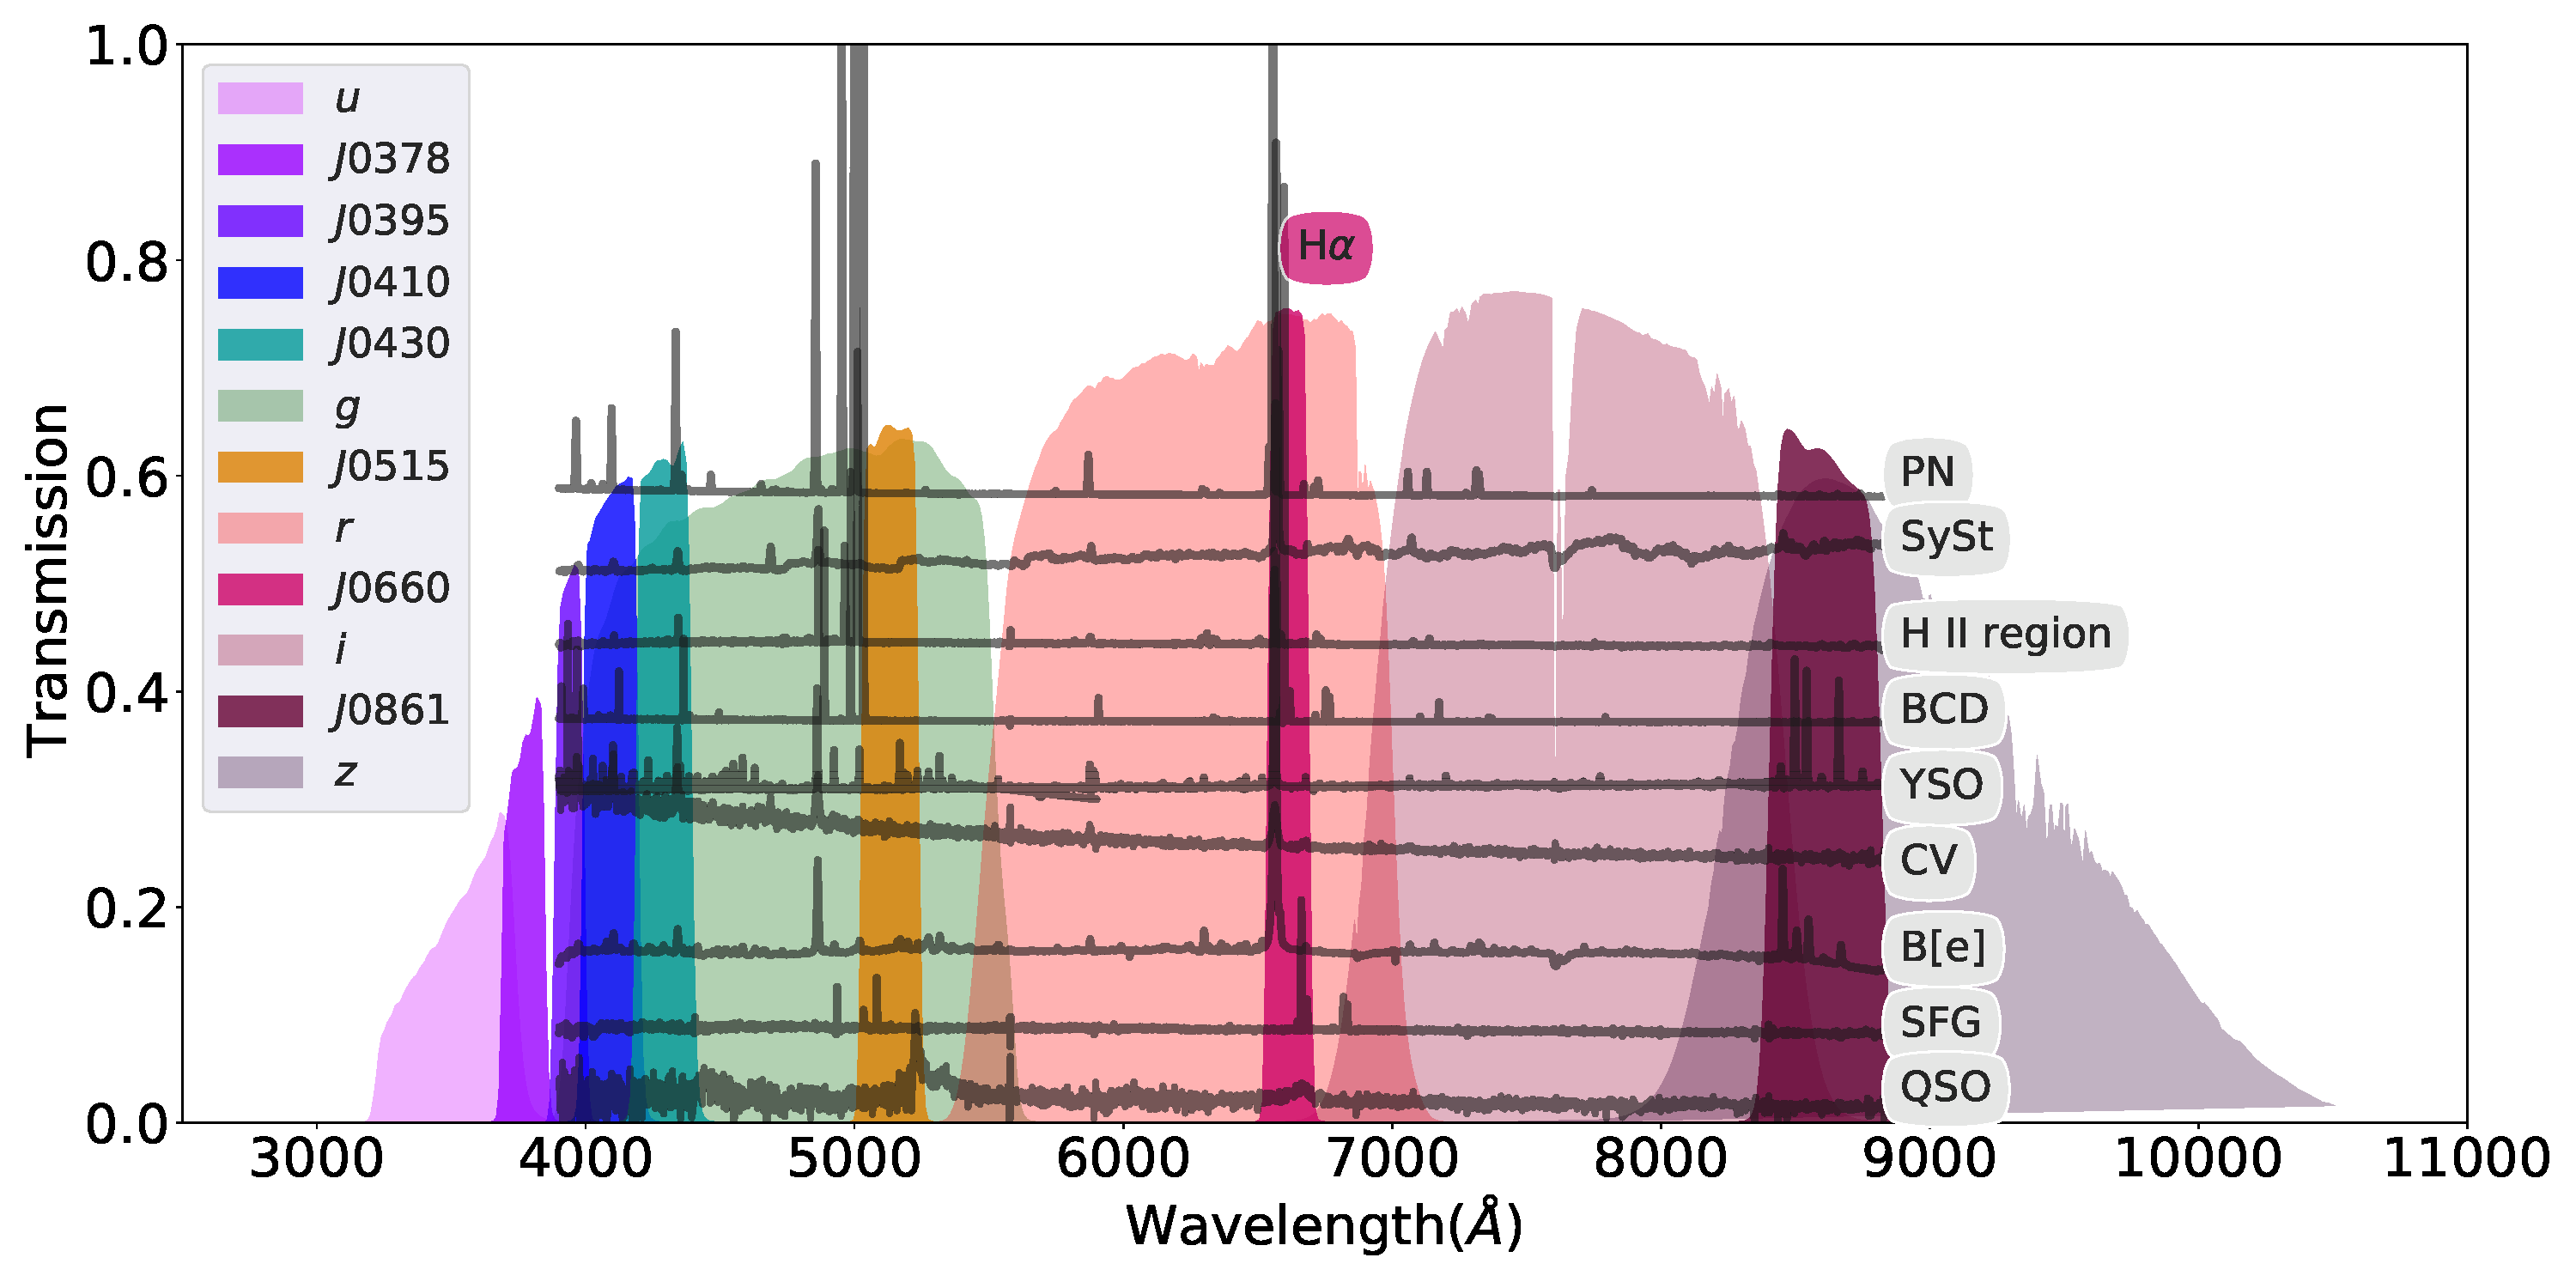
\includegraphics[width=0.9\linewidth]{Figs/splus-filter.pdf}
    \caption{Transmission curves of the S-PLUS filters set. The narrow-band filter
      $J0660$ detects the H$\alpha$ emission line. Over-plotted are different
      classes of emission line objects, from upper to down PN, SySt ... }
    \label{fig:curves}
\end{figure}


\section{Methodology}
\label{sec:metho}

We first constructed a sub-sample from all S-PLUS DR3 from which we
applied an iterative and automatic technique to select objects with
an excess of H{$\alpha$} emission line. Once the objects were selected
we also make a separation of them into two groups those with red and blue
continuum by using optical colors in conjunction with unsupervised
 machine learning statistical tools. These procedures are described below:

\subsection{Initial selection sample}
\label{sec:}

The firts step in our selection procedure consist in the following
criteria to guarantee the quality of the observations of the objects:

\begin{enumerate}
\item The sources must have detection in the filters: $r$, $i$ and
  $J$0660. To assure that we select object must have error minor or
  equal to 0.2 in each of three filters.

\item Must have an $r$ magnitude until $r = 21$.
  
\end{enumerate}

\subsection{Finding the main stellar locus and selecting the H{$\alpha$ emitters}}
\label{sec:}

Once the initial cut were made, we proceed to select the objects with
an excess of H{$\alpha$} wich is represent with a relatively high value of
the filter $J$0660 in comparison with r-band filter. For that we
first divided our sub-sample in for magnitude bins using the $r$-band
magnitudes. The bins have the follow distribution:

\begin{enumerate}
\item  objects with magnitude in the $r$-band $r < 16$
\item  objects with magnitude in the $r$-band $16 \leq r < 18$
\item  objects with magnitude in the $r$-band $18 \leq r < 20$
\item  objects with magnitude in the $r$-band $20 \leq r < 21$
  
\end{enumerate}

To select the emission lines we used the same method created and
implemented by \citet{Witham:2008} its possible to do that because
the S-PLUS has similar filters that the IPHAS project, which are
$r$, $J$0660 and $i$. This technique was used by \citet{Scaringi:2013}
to identify blue objects with excess of H{$\alpha$} and after that
\citet{Wevers:2017} also applied this methodology to create catalogue
of candidate H{$\alpha$} emission showing an high effectiveness. In this
order of ideas we attempted this methodology in S-PLUS.

We first generated the ($r$ - $J$0660) versus ($r$ - $i$) color-color
diagram for each magnitude bins. We then carried a out an initial straight
line fit to all objects in each magnitude bin. This initial fit is an
attempt to find the loci of main-sequence and giant stars. We implemented
a iterative $\sigma$-clipping tecnique to find the best-fitting of the main
stellar locus. In this order of ideas, we made four interactive $\sigma$-clipped.
Once we have found the apropiate fitting for each maginitude bin, we identified
those objects significantly above of this final fit as likely sources with
a excesses of H{$\alpha$}. Objects with a contribution significative of
H{$\alpha$} meet the condition:

\begin{equation}
  (r - J0660)_{\mathrm{obs}} - (r - J0660)_{\mathrm{fit}} \geq C \times \sqrt{\sigma^2_{\mathrm{s}} - \sigma^2_{\mathrm{phot}}}
  \label{eq:criterion}
\end{equation}
 
 where $\sigma_{\mathrm{s}}$ is the root mean squared value of the residuals around
 the fit and $\sigma_{\mathrm{phot}}$ is the error on the observed $(r - J0660)$ colour idex.
 $C$ is a constant which has the value 4 following \citet{Wevers:2017}.
The fits are carried out with the aid of the python library \texttt{astropy.modeling}
\footnote{https://docs.astropy.org/en/stable/modeling/index.html}.

Figure~\ref{fig:criteria-color-plot} ilustrates the procedured used to slected the H{$\alpha$}
emitters in S-PLUS DR3 for each magnitude bin. The continuos black lines represent the initial
fit and  the dashed lines indicate the 4-$\sigma$ clipping fit lines. The dotted lines are
the cut selection criteria for the H{$\alpha$} emitters -- the 4-$\sigam$ above of the final
fit--. Note that theses cut lines are only an approximations because to trace them,
it is only considered the residual around the fit. The actual selection criteria used here
also include the phothometric uncertainties in $r$ - $J$0660 for each individual data source as
shows on the Equation~\ref{eq:criterion}.

\begin{figure*}
  \setlength\tabcolsep{0pt}
  \setkeys{Gin}{width=0.5\linewidth}
  \begin{tabular}{ll}
    (a) & (b) \\
    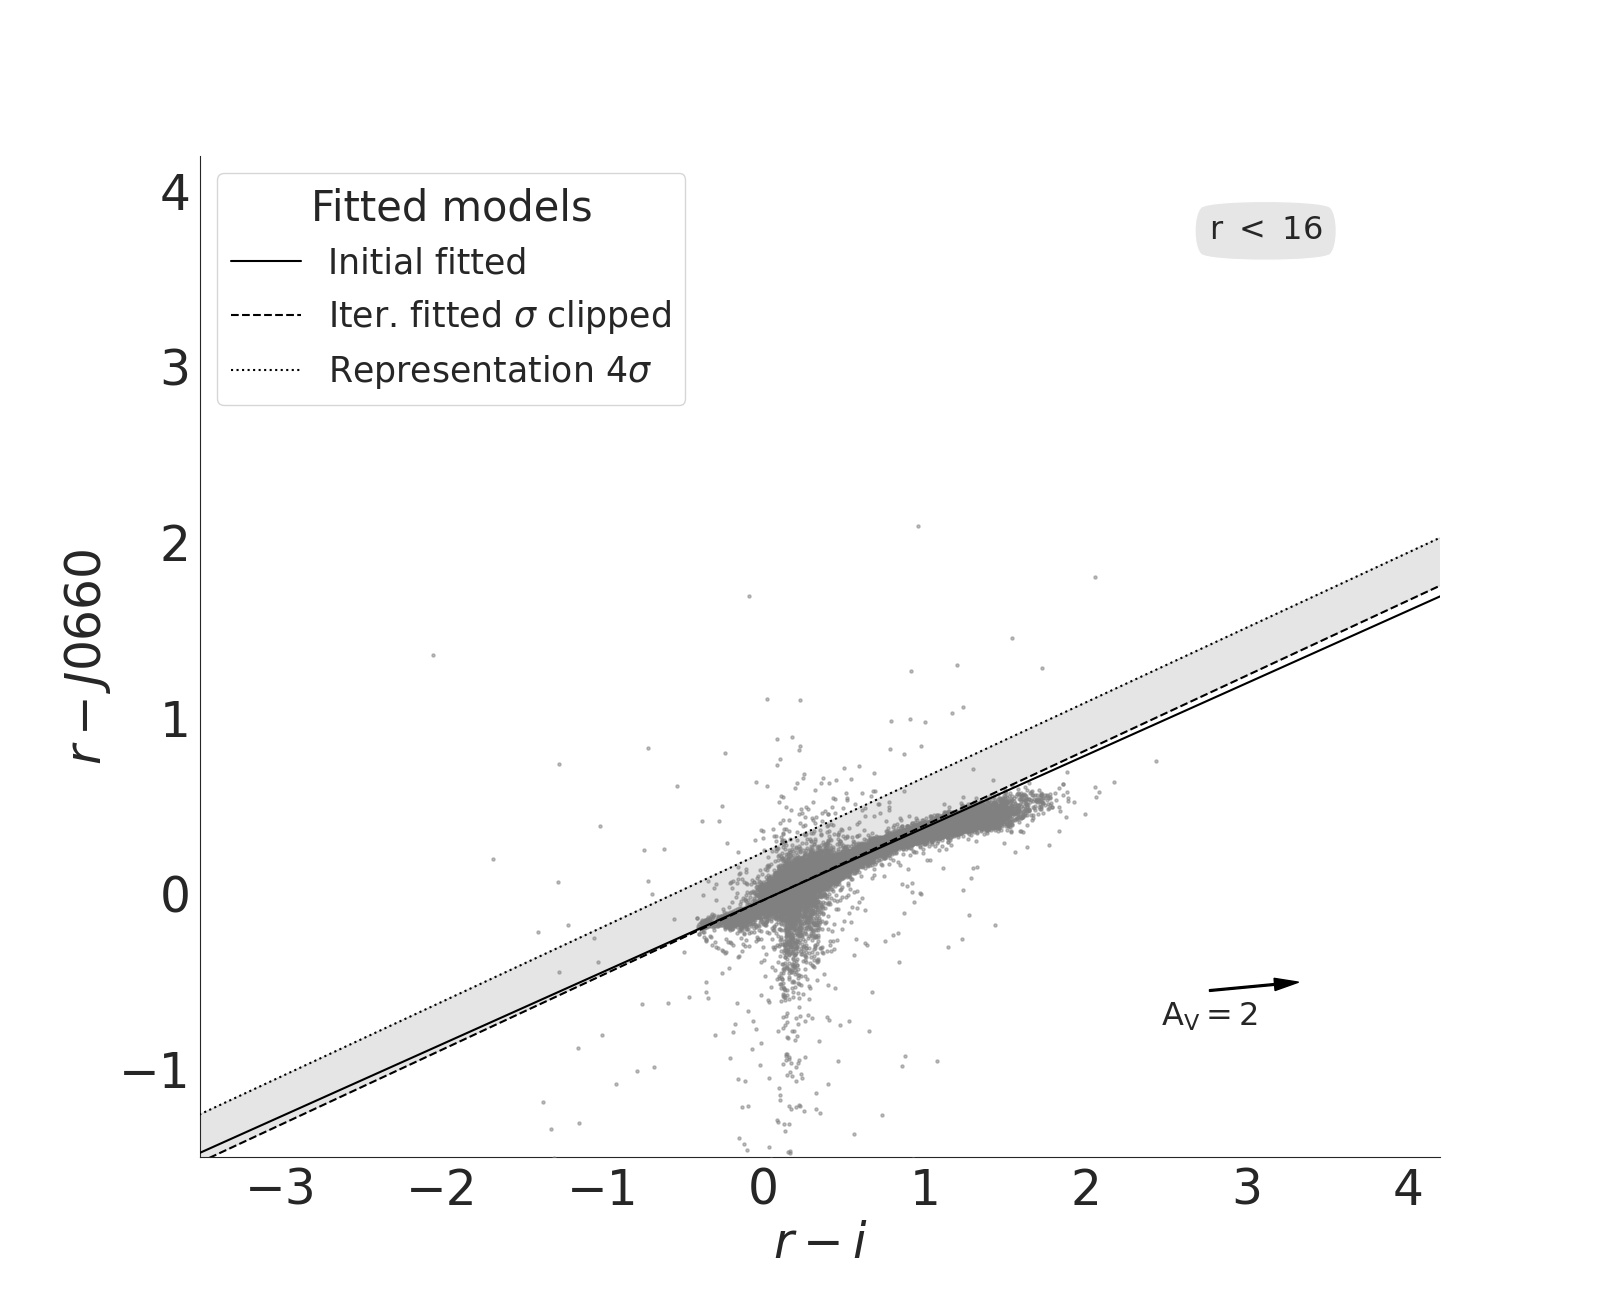
\includegraphics[trim=10 0 65 20, clip]{Figs/diagram-DR3-errorFlag0-3f-16r}
    & 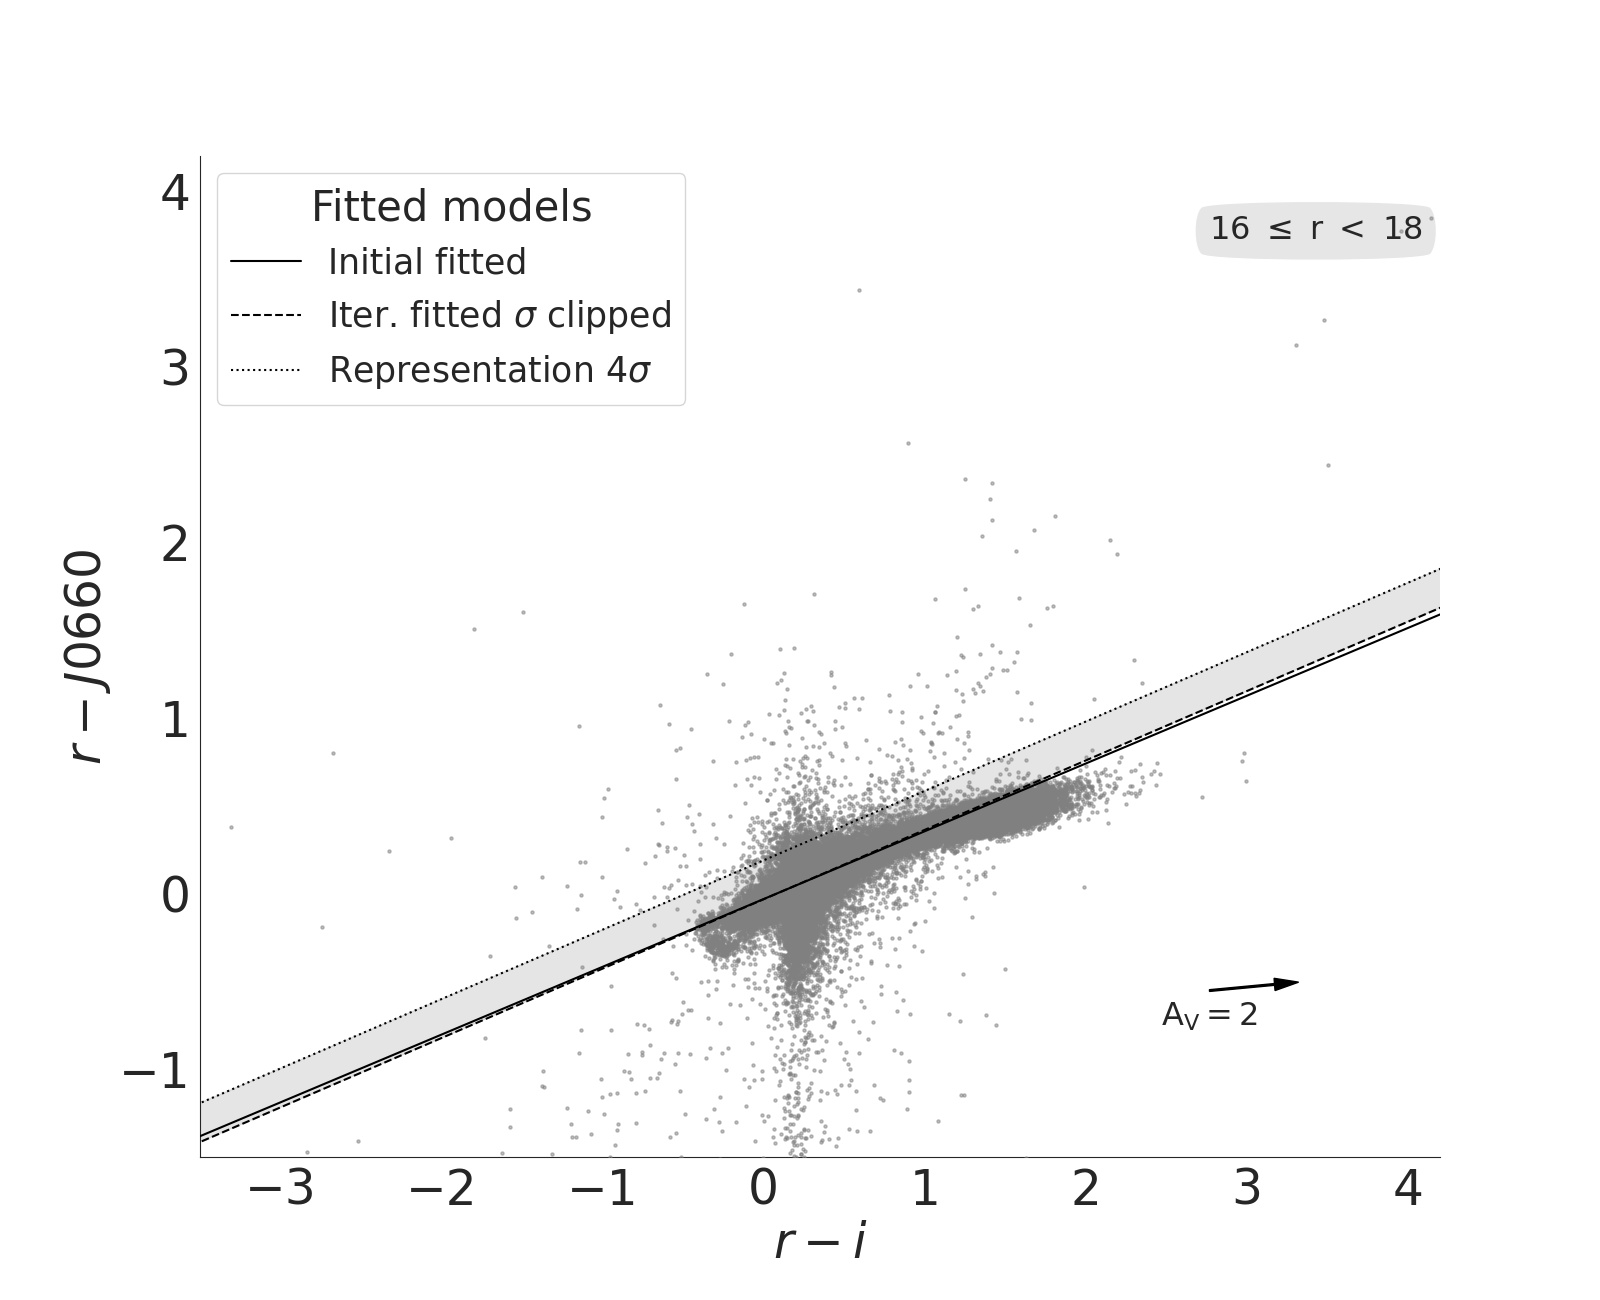
\includegraphics[trim=10 0 65 20, clip]{Figs/diagram-DR3-errorFlag0-3f-16r18}\\
    (c) & (d) \\
    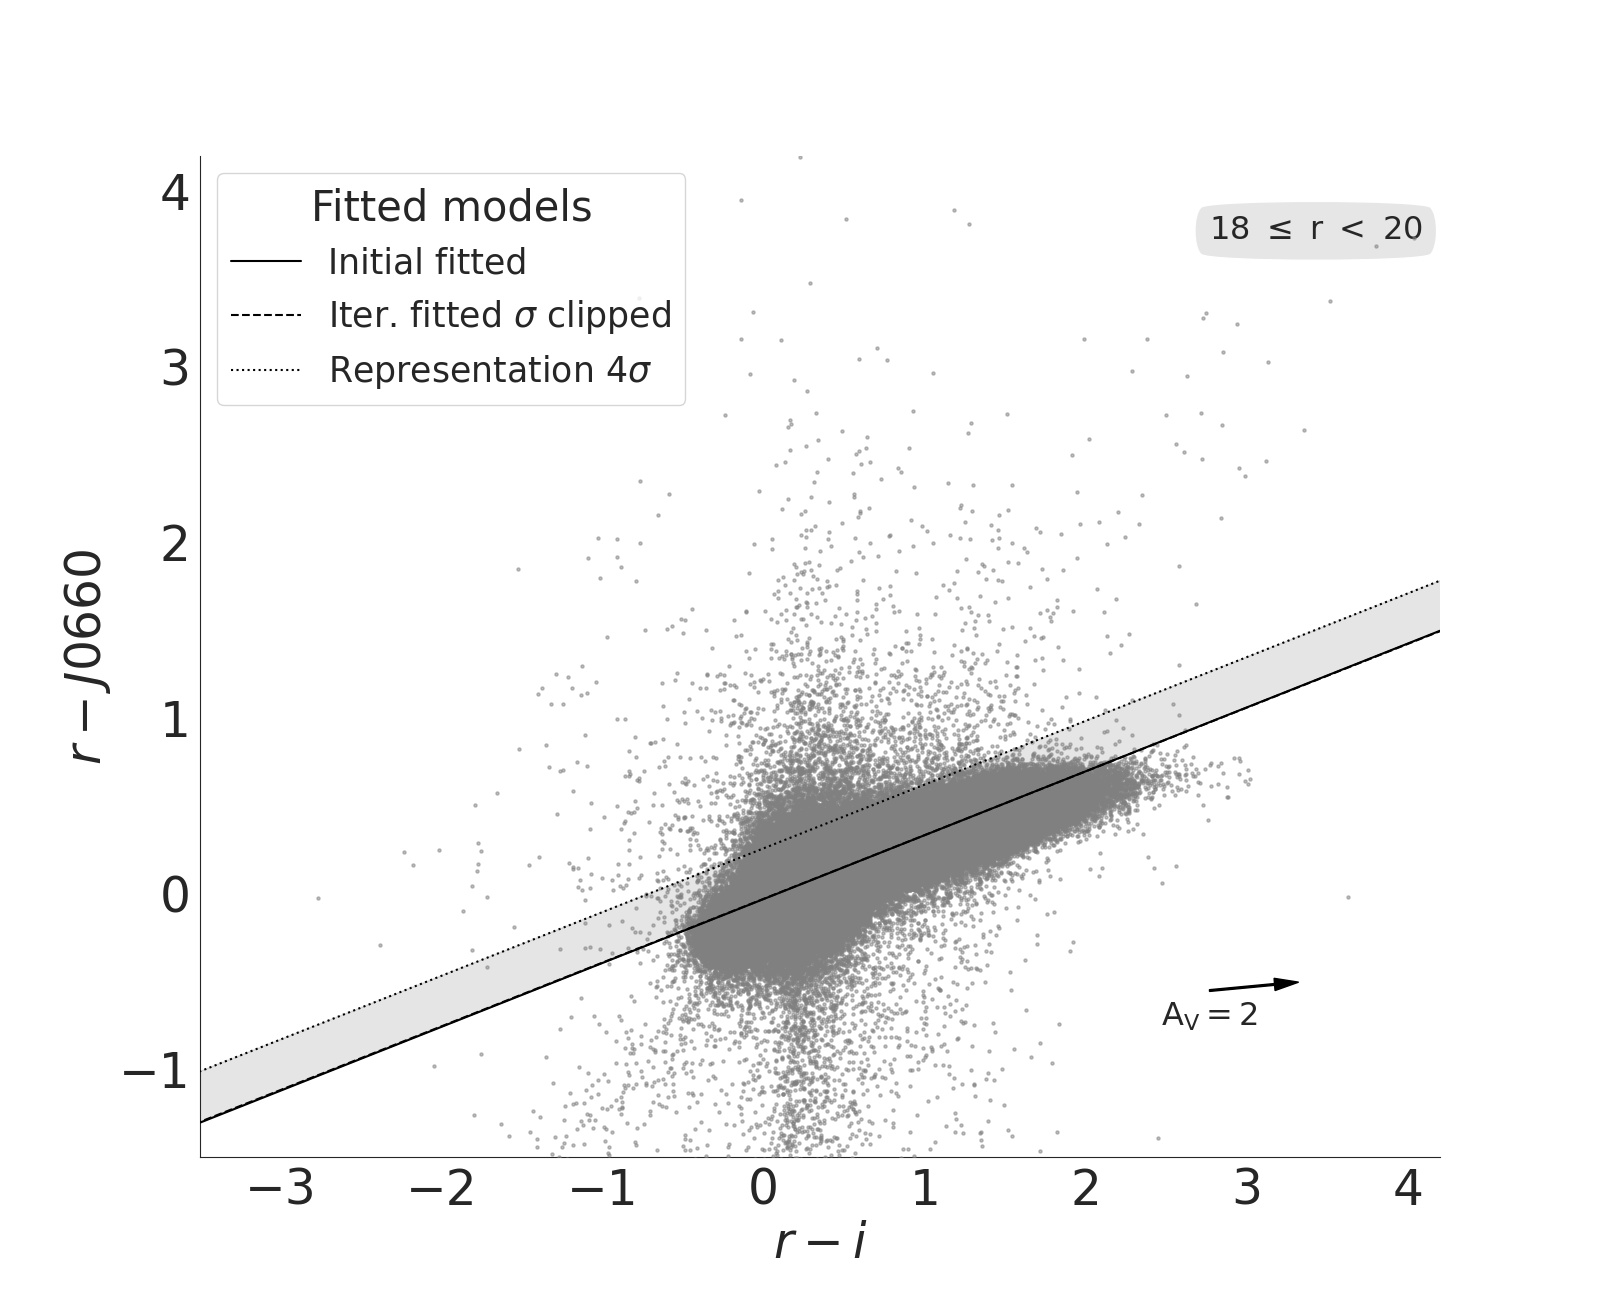
\includegraphics[trim=10 0 65 20, clip]{Figs/diagram-DR3-errorFlag0-3f-18r20}
    & 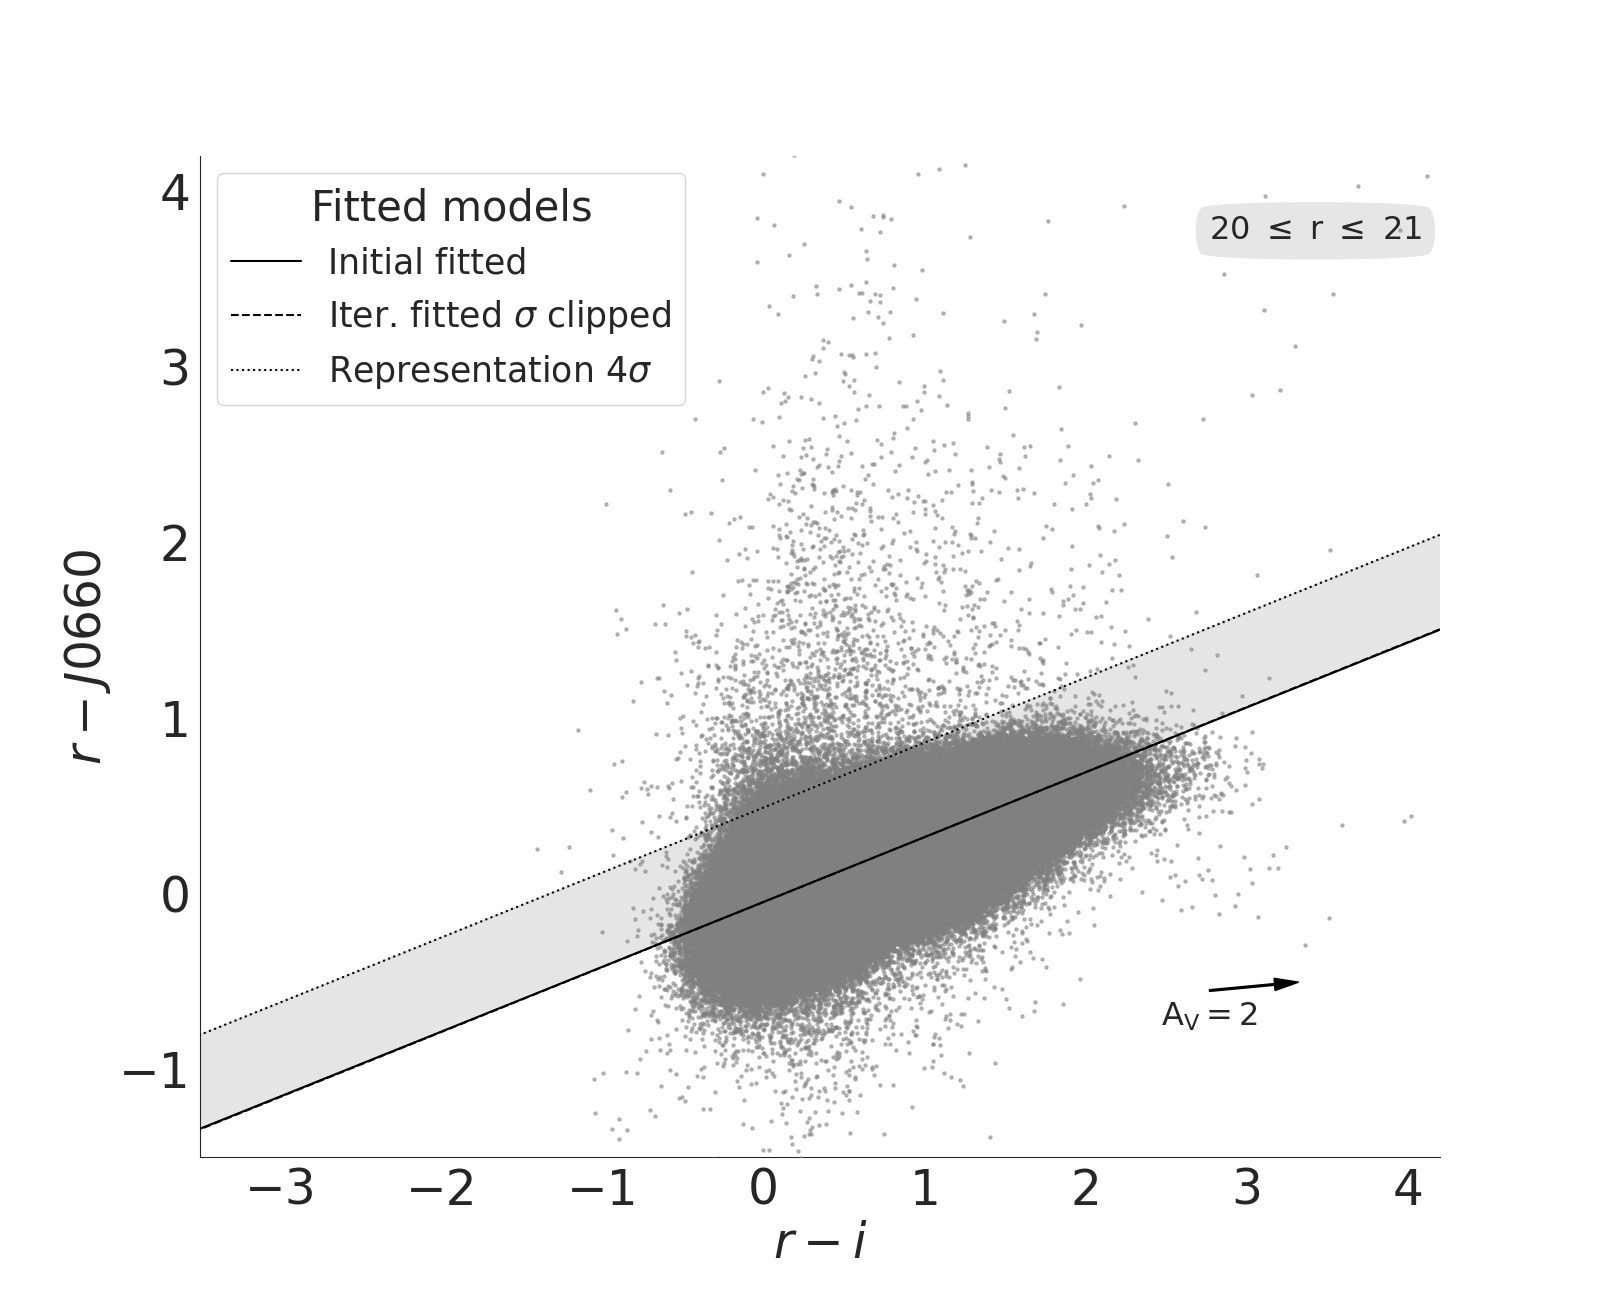
\includegraphics[trim=10 0 65 20, clip]{Figs/diagram-DR3-errorFlag0-3f-20r21}\\
  \end{tabular}
  \caption{An illustration of the selection criteria used to identify strong
    emission-line objects via colour-colour plots. The data shown here are all from the
    S-PLUS DR3. The data are split up into four magnitude bins, as shown in the four
    panels. Objects with H{$\alpha$} excess should be located near the top of the
    colour-colour diagrams. The thin red lines illustrate the original linear
    fit to all the data (grey points). The dashed lines represent the final
    fits to the stellar locus of points which were obtained by applying an iterative
    $\sigma$-clipping technique to the initial fit. The actual cuts used to select
    H{$\alpha$} emitters are shown by the dotted lines. Objects selected as H{$\alpha$}
    emitters must be located above. Note that the cut lines (selection criteria) shown
    here are only approximate, as the actual selection criterion also considers the
    errors on each source. This means that an object could be in the bottom
    right-hand panel is not selected despite clearly lying above the cut line
    ({\sc explicar esta última frase mejor}).}
  \label{fig:criteria-color-plot}
\end{figure*}

After the algorithm was applied to all data, we visually inspection-ed the
resulting list by seeing the S-spectra and corresponding colored image.
The figure~\ref{fig:Spectra} shows an example of how looks like a
S-spectra\footnote{S-spectra signify the S-PLUS emission in flux
or magnitude unities of an object in all twelve bands.} of sources in
magnitude unities selected with methods explained above. This object
clearly exhibits strong H$\alpha$ emitter.

\begin{figure}
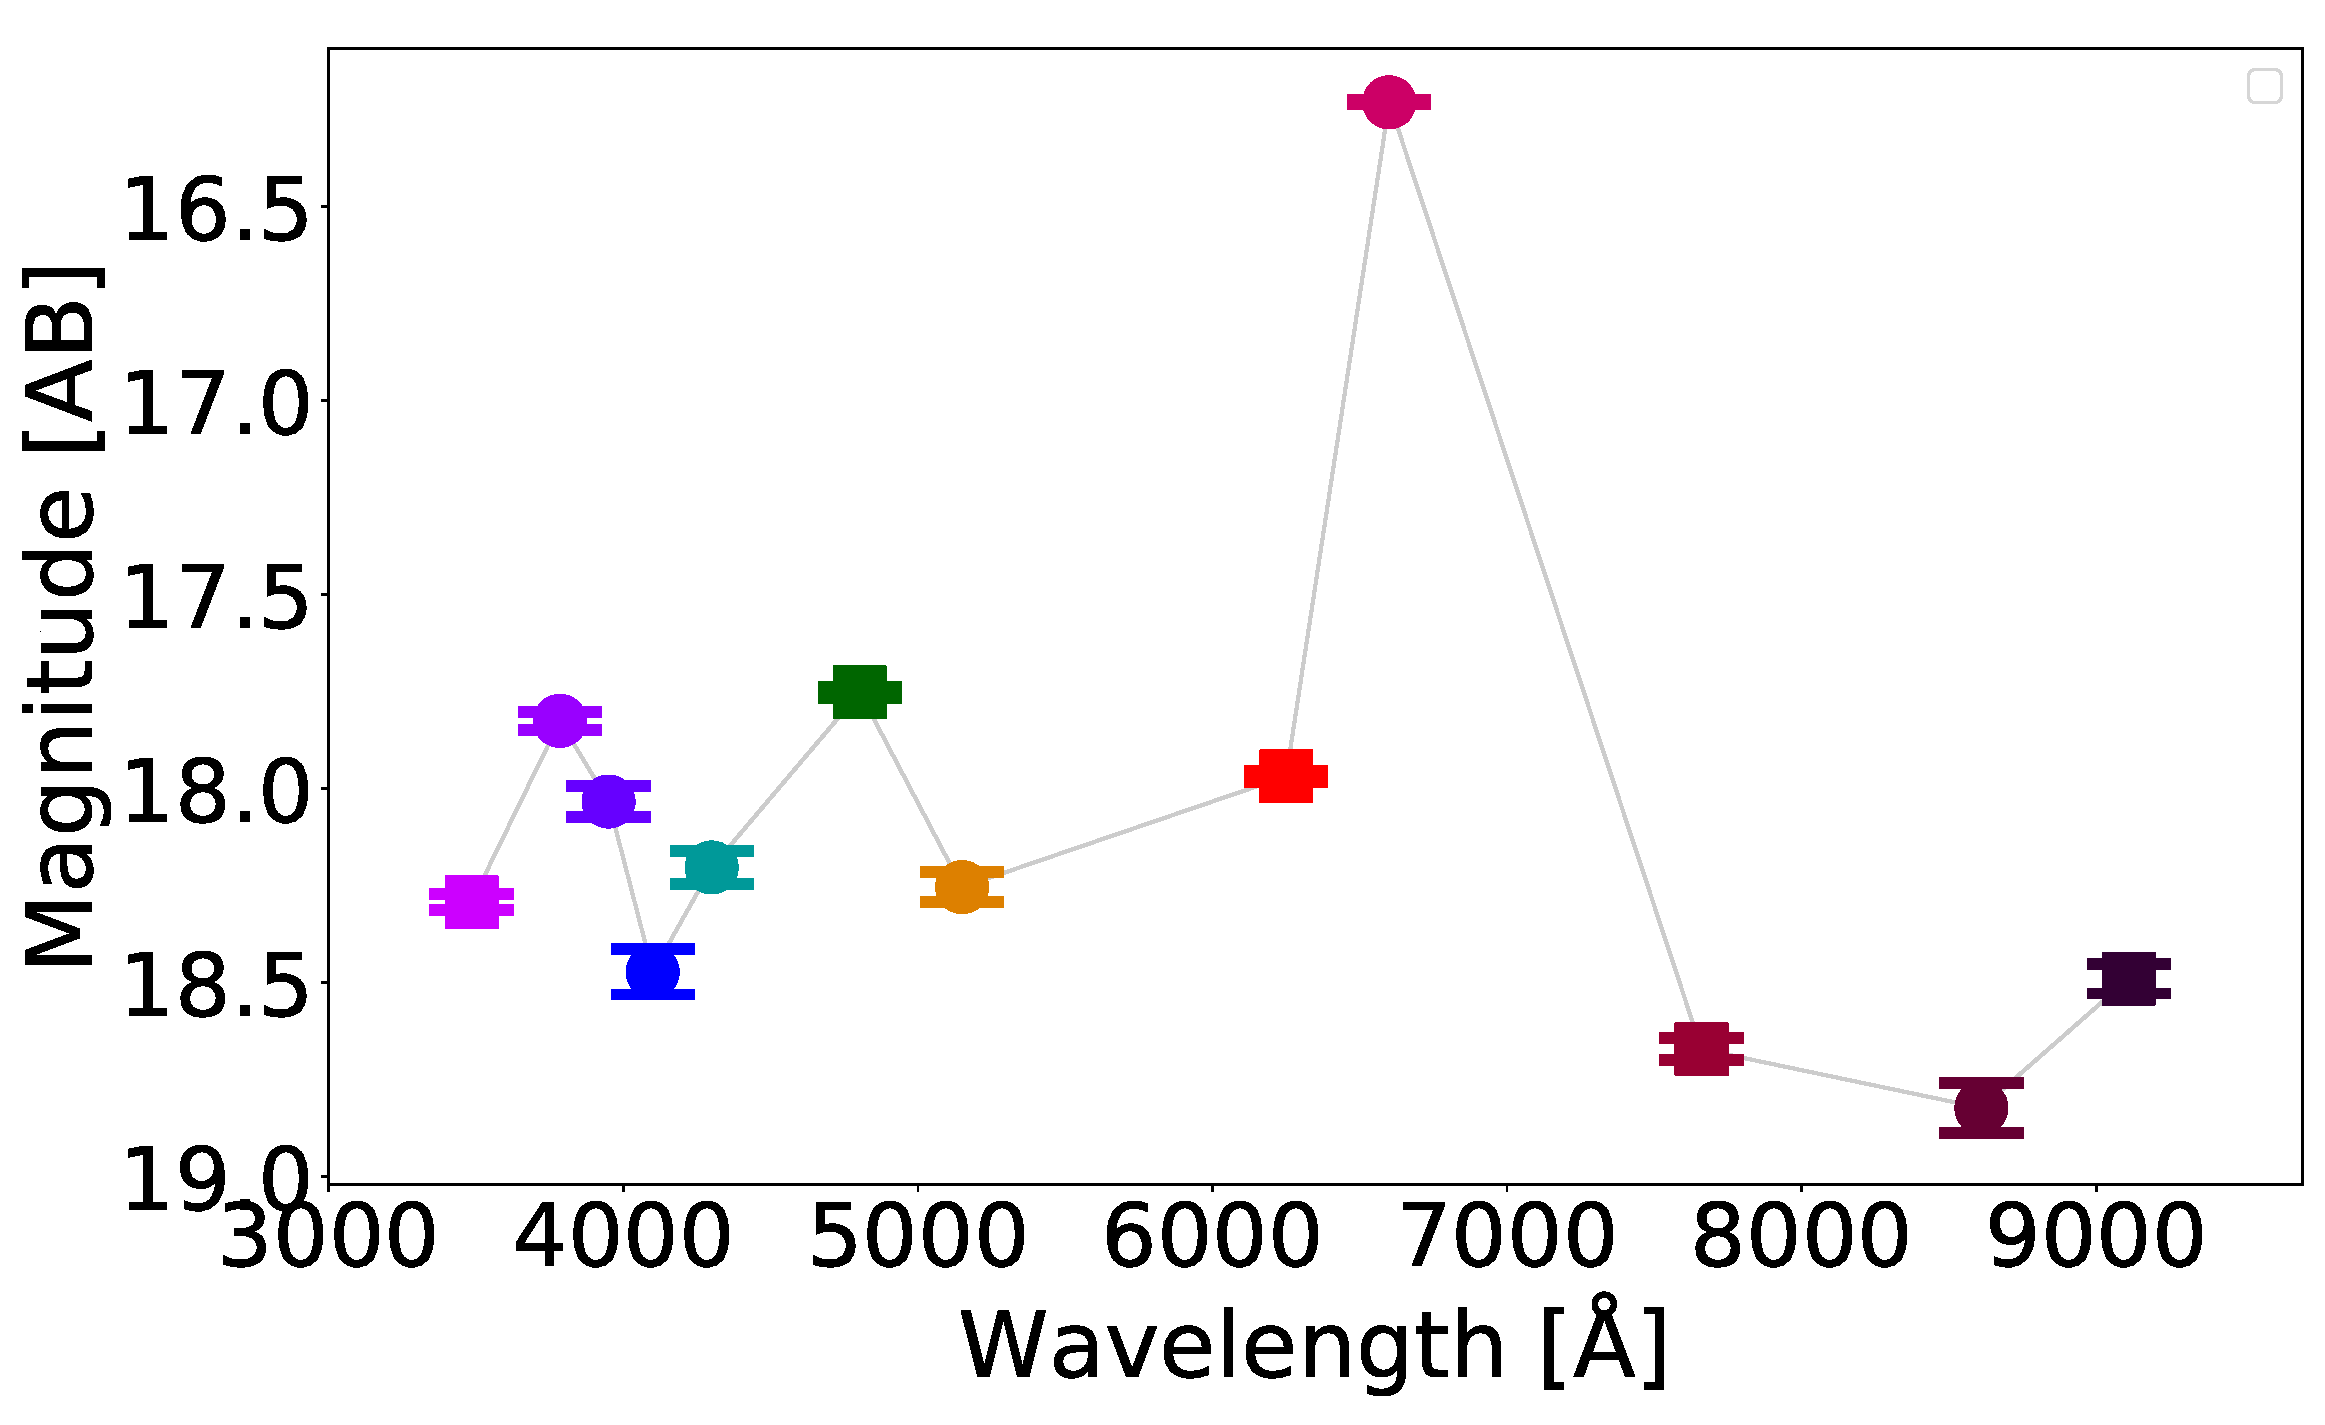
\includegraphics[width=0.9\linewidth]{Figs/photopectrum_splus_HYDRA-0026-052331_Good-LD-Halpha-DR3_noFlag_merge-takeoutbad-Final_PStotal.pdf}
\centering
\llap{\shortstack{%
        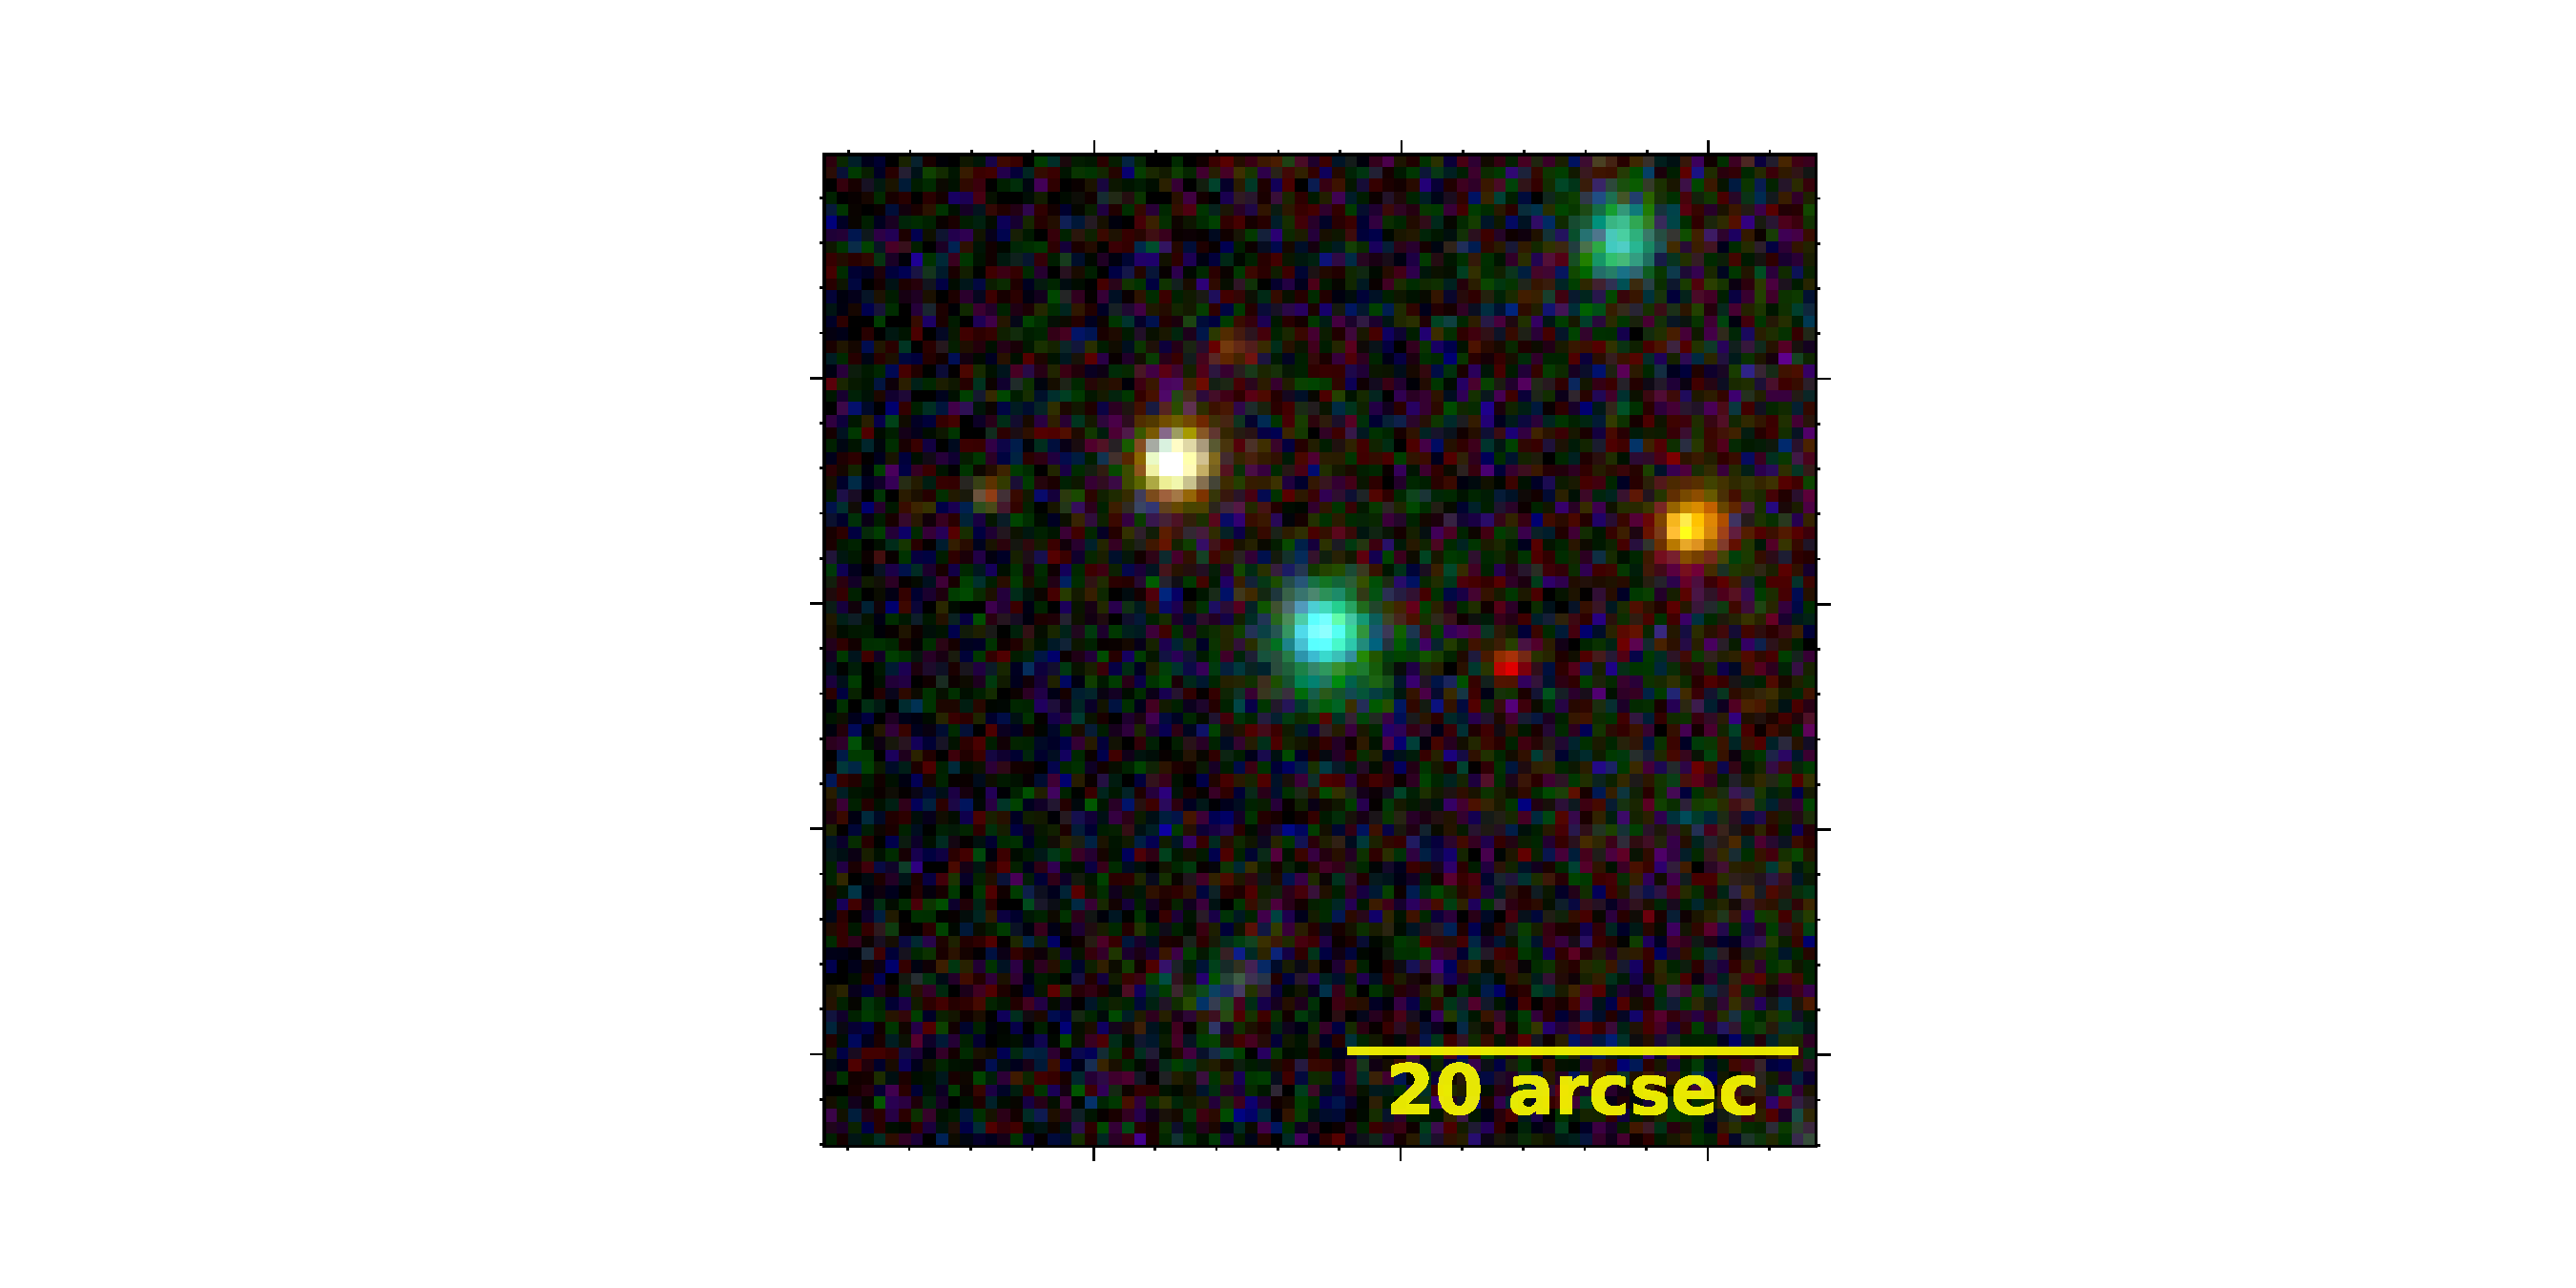
\includegraphics[width=0.25\linewidth, trim=350 10 350 20, clip]{Figs/HYDRA-0026-052331_158.85933642579576--24.753136157195524_80_r.pdf}\\
        \rule{0ex}{0.87in}%
      }
  \rule{0.06in}{0ex}}
\caption{S-spectra of a random object of the emission line objects. Squares represent
  the SDSS-like broad-band filters. From left to right they are \(u, g, r,
  i~\text{and}~ z\). Circle symbols are the narrow-band filters, which from
  left to right represent \textit{J}0378, \textit{J}0395, \textit{J}0410,
  \textit{J}0515, \textit{J}0660 and \textit{J}0861.}
\label{fig:Spectra}
\end{figure}


\begin{figure*}
	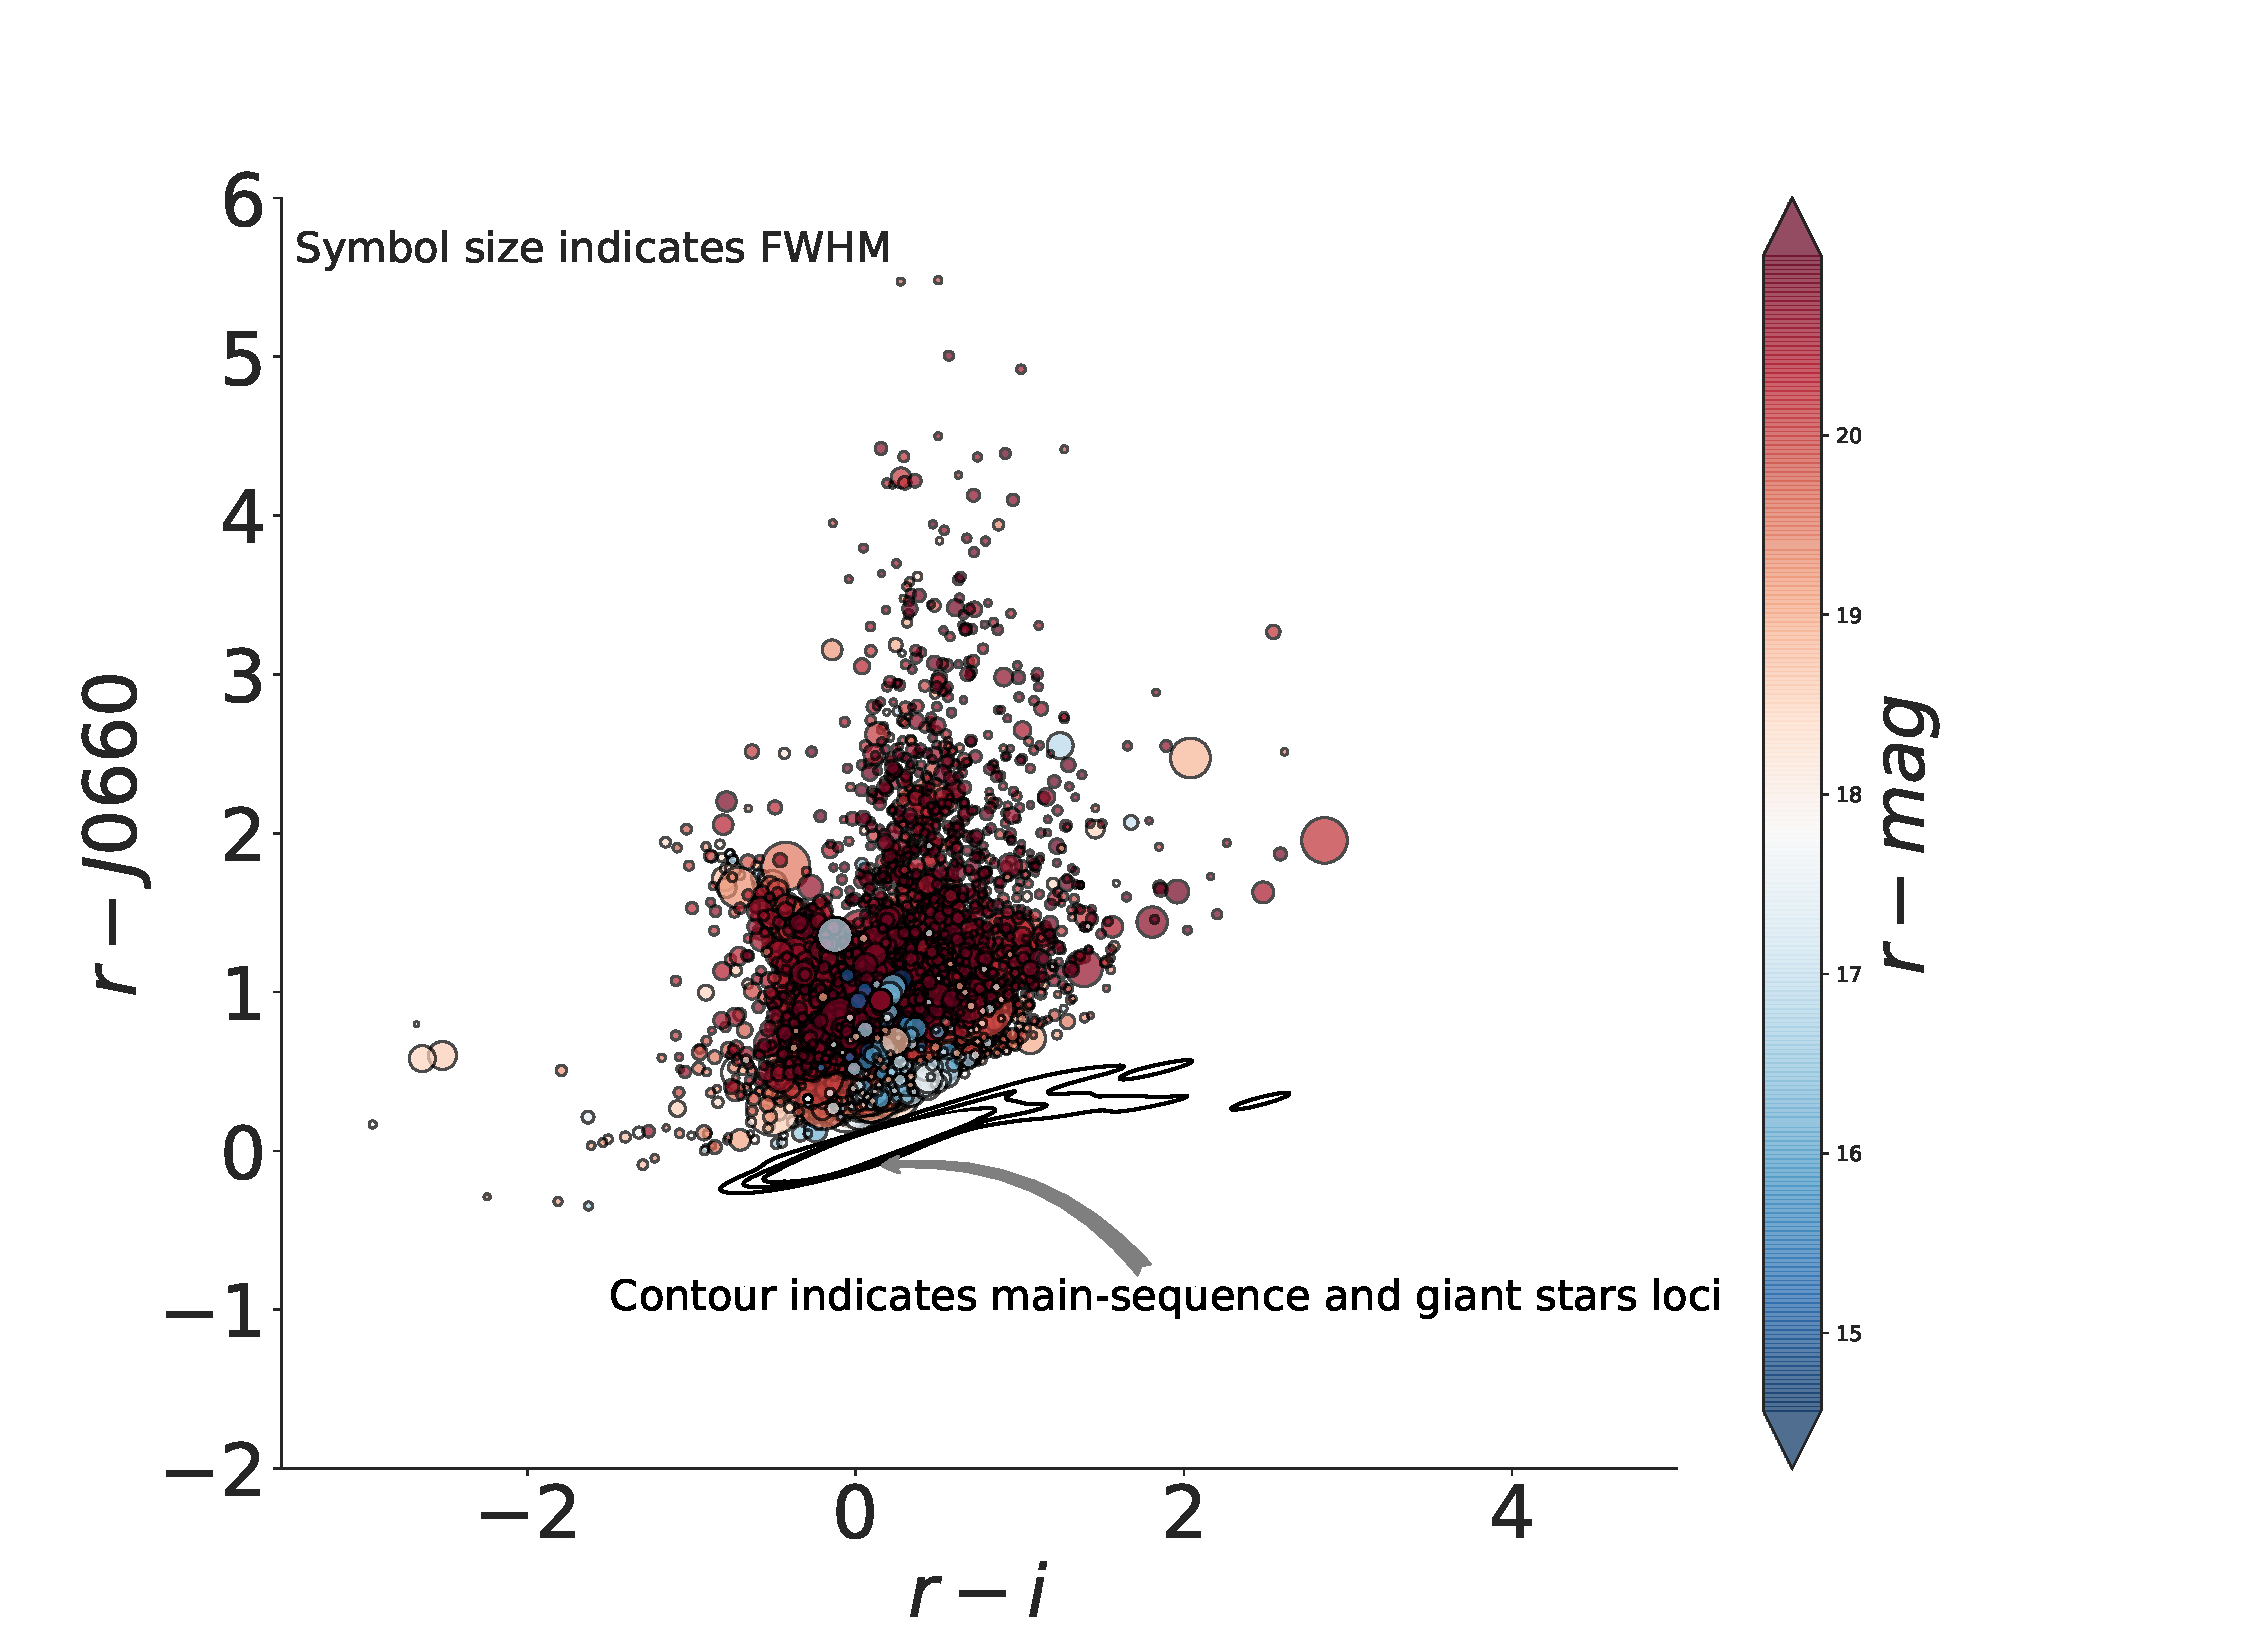
\includegraphics[width=0.9\linewidth]{Figs/final-emitters.pdf}
        \caption{Colour-colour diagram with all the emission line objects selected
          from S-PLUS DR3. Size of the symbols represent the measured FWHM assuming
          a Gaussian core (for more detail see \citealt{Fernandes:2021}). Colored
          bar indicates the magnitude values in the r-band. The contours represent
          the synthetic main-sequence and giant stars loci from the library of stellar
          spectral energy distributions of \citet{Pickles:1998}.}
    \label{fig:emission}
\end{figure*}

Fig~\ref{fig:emission} exhibits the distribution of the emission on the
$r - J0600$ versus $r - i$ color-color plane. At this point we can say that
the algorithm implemented works well in selected objects with a excess in emission
on the $J$0660 filter. It is possible to affirm that, because the identified objects
are located  above of the loci of the main and giant stars. The S-PLUS synthetic  photometry
of the stellar locus is represent by the contours in the diagram and was obtained by using the
filter transmission profiles, shown in Fig.~\ref{fig:curves}, and the library of stellar
spectral energy distributions of \citet{Pickles:1998}. This synthetic magnitudes were
defined in the AB magnitude system \citep{Oke:1983}. The wide distribution of fonts across
the colors $ r - J060 $ and $ r - i $ indicates that several types of objects were selected.
For instance, higher values on the  $r - J060$ color of some sources could be indicating
that they are H II regions or/and blue compact galaxies and PNe. On the hand, the 
$r - i$ color indicates the rendered sources such as SySt and young stellar objects
or source with strong blue continuum as cataclysm variables.

\begin{figure*}
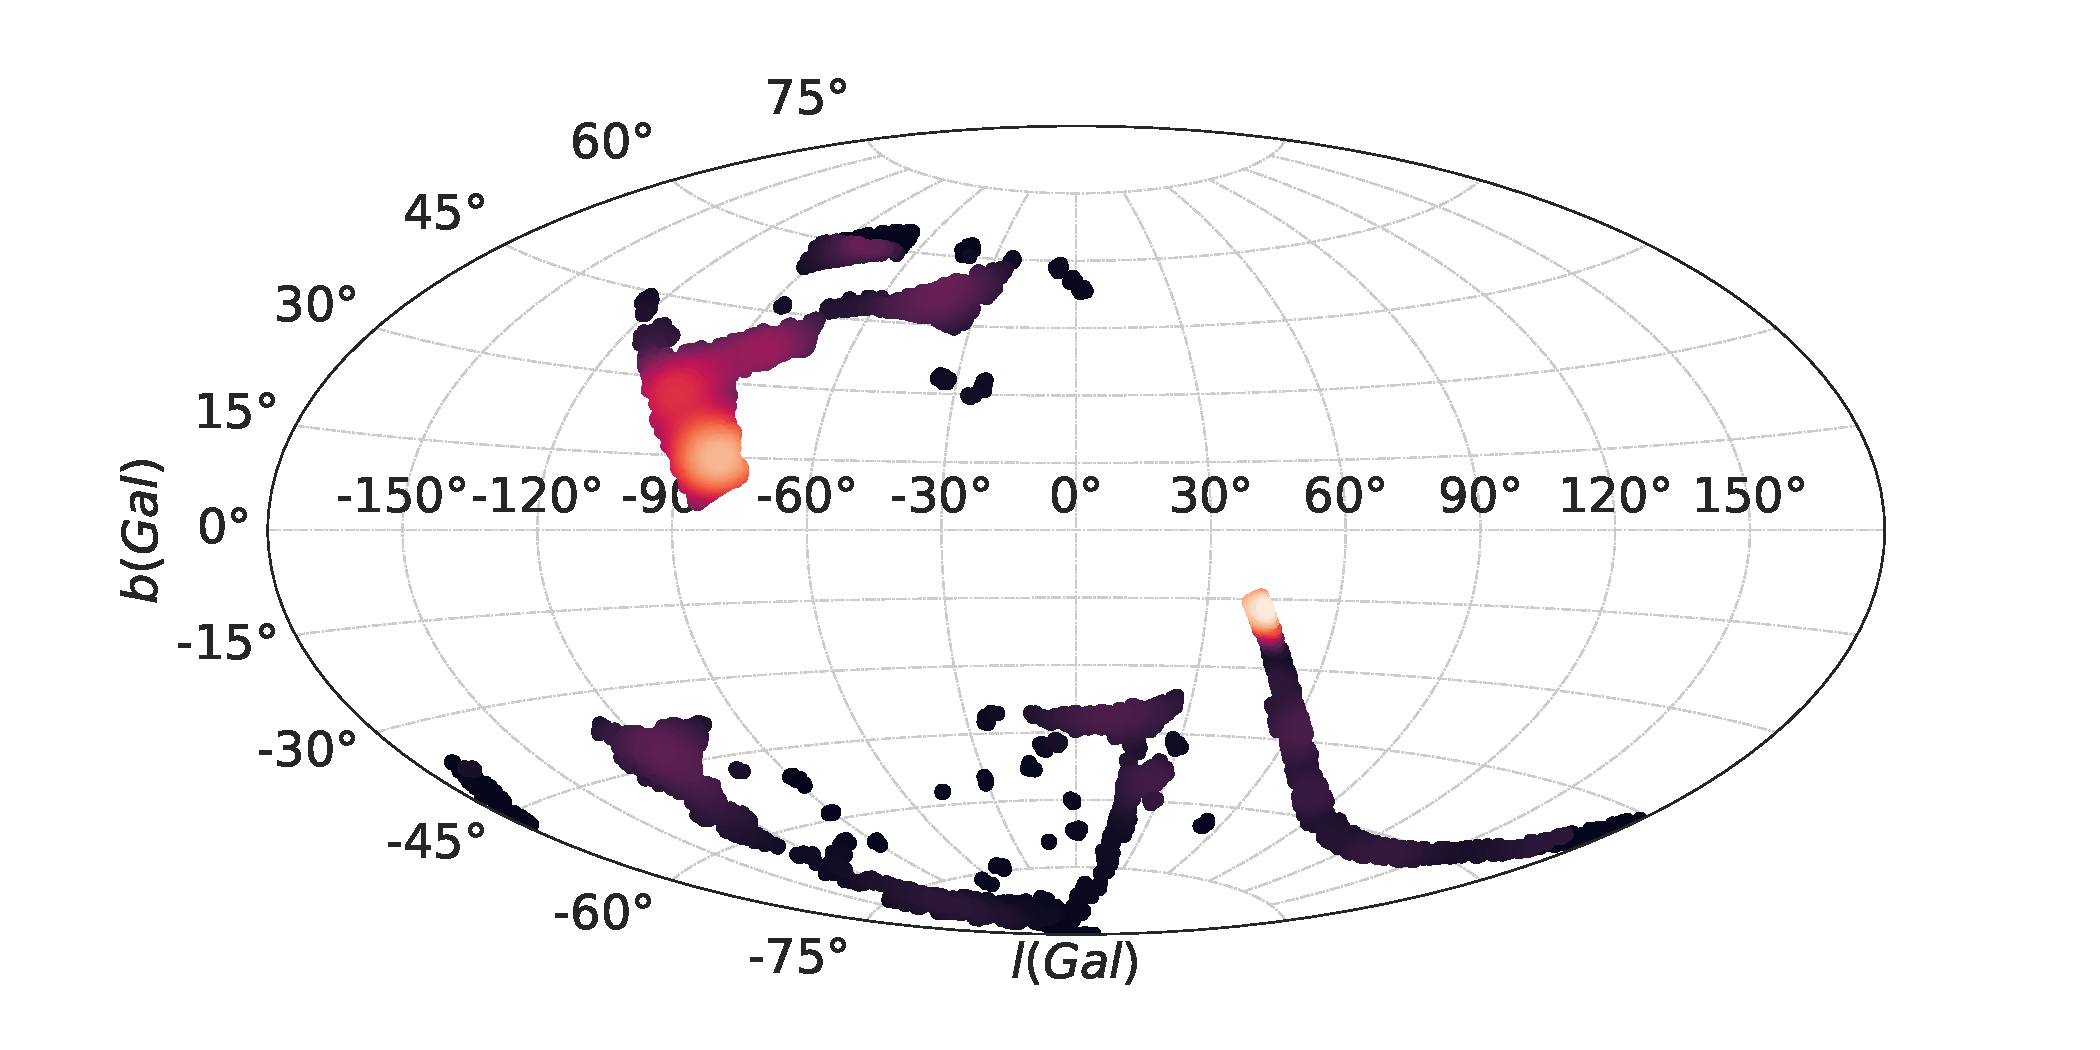
\includegraphics[width=0.9\linewidth]{Figs/halpha-emitters-galactic-aitoff.pdf}
\centering
\llap{\shortstack{%
        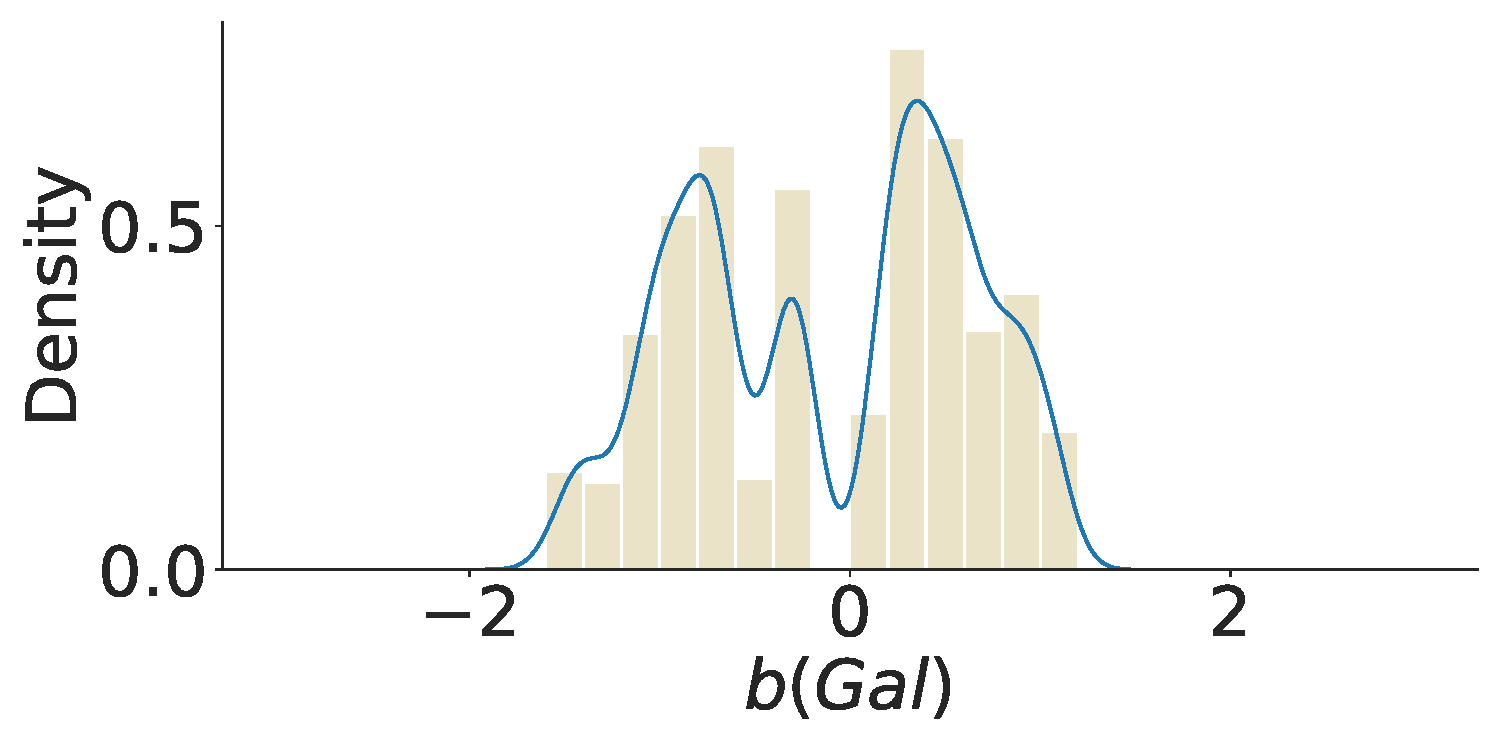
\includegraphics[width=0.25\linewidth, trim=10 10 -40 0]{Figs/distribution-bgalactic.pdf}\\
        \rule{0ex}{1.8in}%
      }
  \rule{1.0in}{0ex}}
\caption{Distribution of H{$\alpha$} emitters in Galactic longitude and latitude
  coordinate. Inset figure represents distribution of the objects in Galactic latitude.}
\label{fig:aitoff-distribution}
\end{figure*}

Fig.~\ref{fig:aitoff-distribution} displays the distribution of all emitters in Galactic la
ic latitude and longitude. The density map regions represent the spatial positions of the objects
on the sky. The surface density of $J$0660-excess objects is highest near the Galactic plane.

Once, we felt confident of our sample of H{$\alpha$} emission lines sources,
we proceeded to classify the objects into two big groups; one group containing those
objects with a strong blue continuum and another with an intense emission of the
continuum on the blue part of the spectrum. 


\subsection{Unsupervised machine learning/clustering techniques}
\label{sec:clustering}

In this work we are using unsupervised machine learning approaches to divided our sample
in two groups: one represent the blue sources and the another one are the red sources.
The blue are those that have strong emission of the continuum on the part blue of the
spectra and the another with strong emission continuum of the red one. For that task,
was implemented two clustering techniques; hierarchical clustering and Hierarchical
density-based cluster selection based on the $(g - r)$ and $(z - g)$ colors.

\subsubsection{$(g - r)$ versus $(z - g)$ color-color diagram}

\begin{figure}
	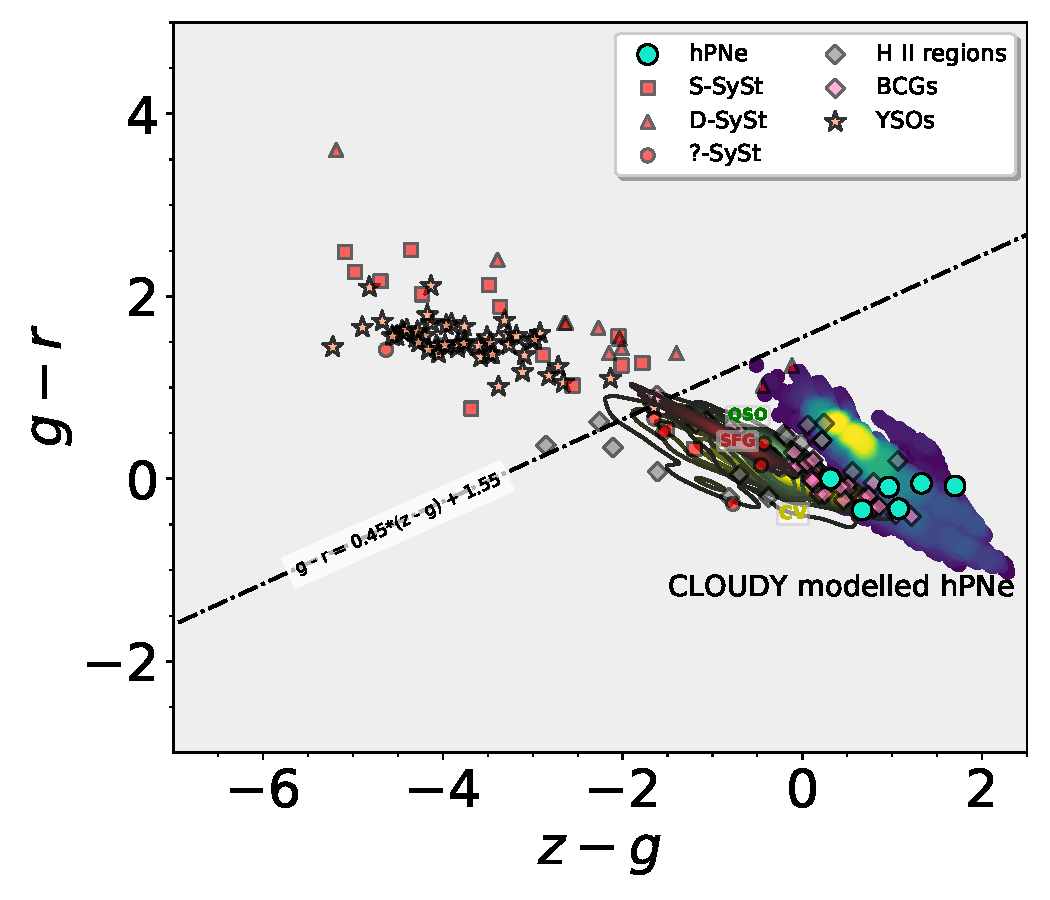
\includegraphics[width=0.9\linewidth]{Figs/Fig-SPLUS-gr-zg.pdf}
        \caption{The $(g - r)$ versus $(z - g)$ synthetic color-color diagram of
          several classes of emission lines objects. Included in the diagrams, there
          are families of CLOUDY modelled hPNe spanning a range of properties (density
          map region). Cyan circles represent S-PLUS photometry from observed spectra
          Grey diamonds represent H II regions in NGC 55. Red
          boxes display symbiotic stars, this group also includes Galactic and
          external SySt from NGC 205 IC 10 and NGC 185,. Yellow circles correspond to
          cataclysmic variables (CVs) from SDSS. Pink circles indicate  blue compact
          galaxies (BCGs) from SDSS. Orange triangles refer to SDSS
          star-forming galaxies (SDSS SFGs). SDSS QSOs at different redshift
          ranges are shown as light blue diamonds, and YSOs from Lupus and
          Sigma Orionis are represented by salmon stars. The diagonal line represent
         a subjective criterion to separate the objects into two color types.}
    \label{fig:synthetic}
\end{figure}

In order to find the best color-color diagram to separating the final sample of
emission line objects into two color types, we first attempted constructed  color-color
diagrams by using the S-PLUS simulated photometry of several classes of emission line
objects\footnote{It is important to note that there are other classes of objects
with emission lines that have not been included, because our main objective is to
separate between two types of these objects by their photometric colors.}.
The {$(g - r)$ versus $(z - g)$ color-color diagram is displayed on
  the Fig.~\ref{fig:synthetic}. The SySt span a wide range on the $(z - g)$ color,
  from approximately -0.5 to 6.0. This wide range on the color may refer to the different
  type spectral of the cold stellar component of the binary system. All the YSOs and many
  SySt are located on the top-left on the diagram indicating a reddening effect of the
  circumstellar disk for many SySt (for example for those symbiotic with a Mira star)
  and YSOs. On the other hand, the PNe, HII regions, CVs, QSOs and emission line galaxies
  are located on the lower-right region in the diagram. This indicates blue continuum
  present in each classes of theses objects, mainly by the presence of the high excitation
  star, for instance, white dwarf in planetary nebulae and cataclysm variable stars and
  massive young stars in H II regions and the starburst galaxies. Although some SySt are located
  in the region where appear the blue sources, this color-color diagram seems to separate
  very well two color types, blue from red sources.

\begin{figure}
	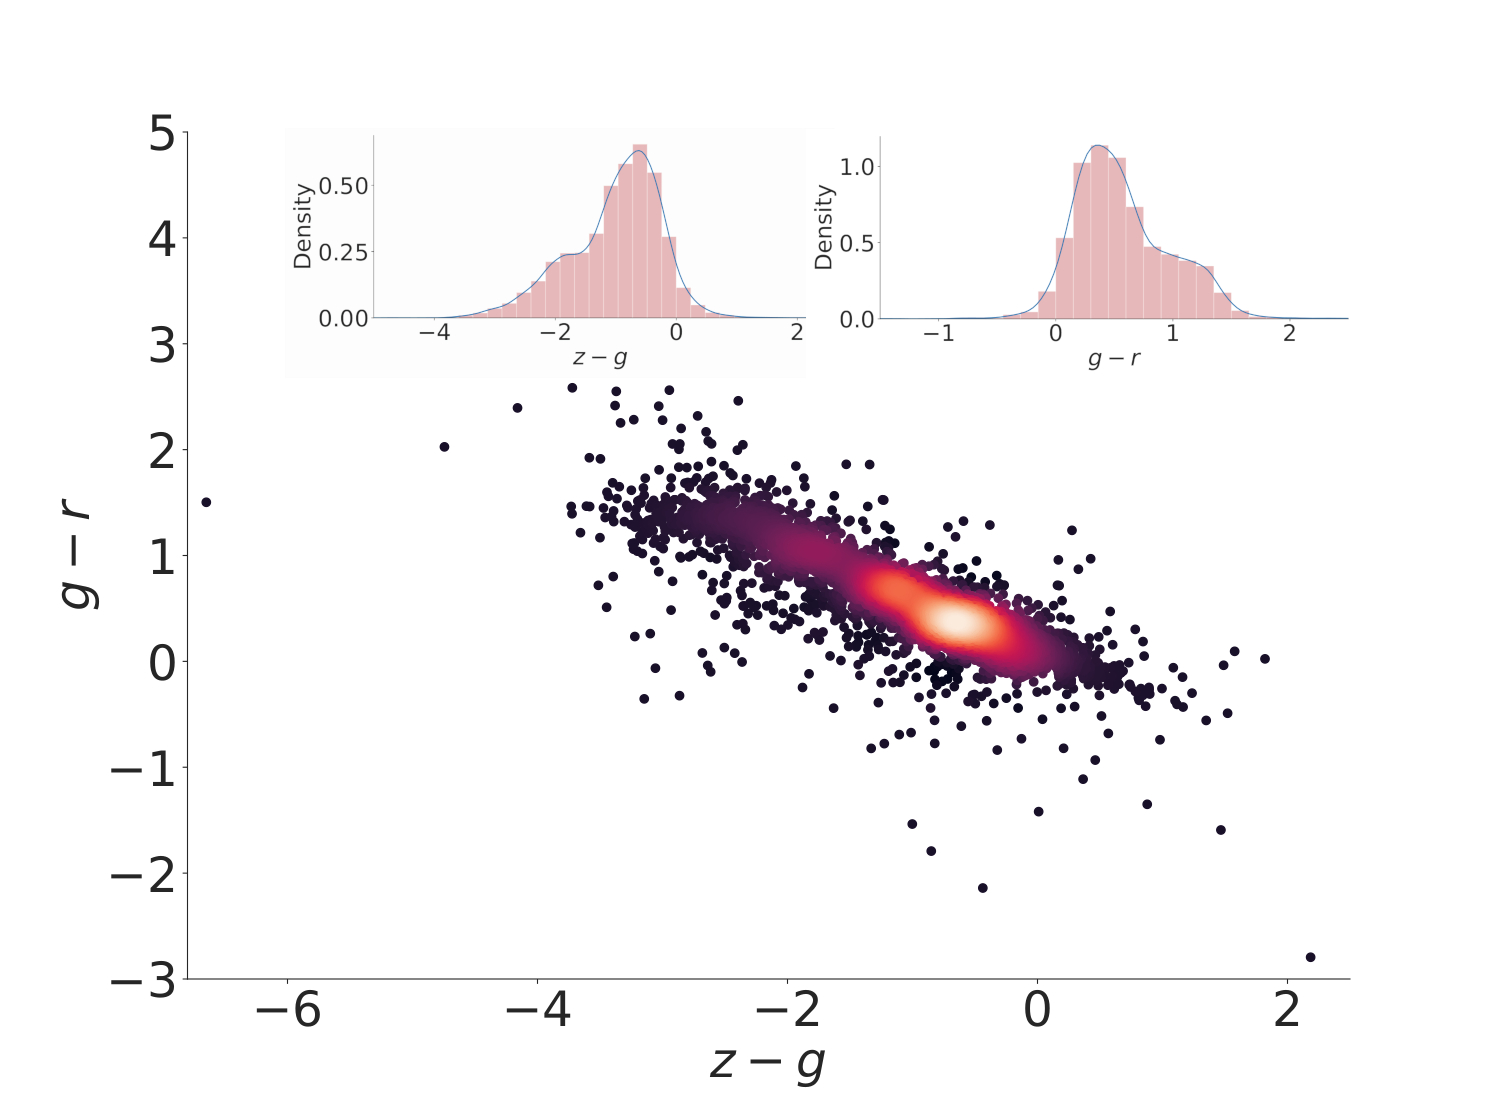
\includegraphics[width=0.9\linewidth]{Figs/red-blue-colorObjects-gr-edit.jpg}
        \caption{The $(g - r)$ versus $(z - g)$ color-color diagram with all the emission line
          objects selected in S-PLUS. The inset figures represent the $(g - r)$ and  $(z - g)$
        distributions.}
    \label{fig:new-color}
\end{figure}


We constructed the $(g - r)$ versus $(z - g)$ color-color diagram using the photometry of
our final list of H{$\alpha$} emitters, which is presented in Fig.~\ref{fig:new-color}.
As was we expected two-color population is showed in the diagram perceptible in the level of the
color of the density region on which yellow areas represent a higher concentration of points. This is re-forced by the bimodal shape of the $(g - r)$ and $(z - g)$ color distributions (see inset
plots of the Fig.~\ref{fig:new-color}). The two peaks of the $(g - r)$ and $(z - g)$
distributions clearly correspond to blue and red sources, respectively. This histograms also
show that the fraction of blue objects is considerable higher than the red ones.

\subsubsection{Hierarchical agglomerative clustering}
\label{sec:Hierar}

Hierarchical clustering belong to the family of clustering algorithms
on which are constructed clusters by merging and splitting them successively.
It is an unsupervised algorithm that yields a dendrogram\footnot{Dendrogram is
a diagram representing tree, which shows hierarchical relationship between objects.}
represents the nested grouping of patterns and the levels of similarity
at which the groupings change \citep{Jain:1999}. There is two type of hierarchical
clustering: one is the \textit{hierarchical agglomerative clustering} (that we have
used in this work) which is ``bottom-up'' approach. Hierarchical agglomerative
clustering (\texttt{HAC}) consists of building a binary merge tree, starting from 
each data element stored at the leaves (interpreted as individual clusters)
and proceed by merging two by two the ``closest'' sub-sets (stored at nodes)
until it reaches the root -unique cluster- of the tree that contains all the elements
of the data set. Agglomerative term is used  to define it since the individual data
point are successively agglomerated into higher-level. In each  iteration, two cluster
are selected that are considered as close as possible. These cluster are merged and
replaced with a newly created merged cluster. Thus, each merging step reduces
the number of cluster by ``1''. Therefore, the method needs to be designated for
measuring proximity between cluster containing multiple data points, so that
they may be merged \citep{Mann:2013, Aggarwal:2015}. We could describe how to
work the algorithm in three simple steps:

\begin{enumerate}
\item Initially, each data point represents the clusters i.e. leaves.
\item It looping merges the nodes (clusters) that have the maximum similarity
  between them.
\item At the end of the process all the nodes belong to an unique cluster. This is
  known as the root of the tree structure.
 \end{enumerate}


The other type is the \textit{hierarchical divisive clustering}. This is a ``top-down''
approach. The data start in one cluster (the root of the tree), and splits step by step
are performed recursively as one moves down the hierarchy. It is the inverse procedure
of \texttt{HAC}.

In simple words, hierarchical clustering approaches can be interpreted  as an
algorithm that groups similar objects into groups called clusters or nodes.
The endpoint is a set of clusters, where each cluster is distinct from each other cluster,
and the objects within each cluster are broadly similar to each other.


Choosing the number of cluster. Firstly, the Hierarchical cluster output dendrogram (tree)
can be implemented to obtain the desired clustering. Secondly, the dendrogram schema allows
a convenient way to establish the entity relationship between at all levels of granularity.
In conclusion, a dendrogram is a visualization in form of a tree showing the order
and distances of merges during the hierarchical clustering.

\begin{itemize}
  
     \item On the $x$ axis you see labels. If you do not specify anything else they
       are the indices of your samples in X.
     \item On the $y$ axis you see the distances (of the ``ward'' method in our case).
       
\end{itemize}


\subsubsubsection{Dendrogram Truncation}

As you might have noticed, the above is pretty big for many samples already and you
probably have way more in real scenarios, so let me spend a few seconds on highlighting
some other features of the dendrogram() function:


Starting from each label at the bottom, you can see a vertical line up to a
horizontal line. The height of that horizontal line tells you about the distance
at which this label was merged into another label or cluster. You can find that
other cluster by following the other vertical line down again. If you don't
encounter another horizontal line, it was just merged with the other label
you reach, otherwise it was merged into another cluster that was formed earlier.

Hierarchical clustering can be performed with either a distance matrix or raw data.
When raw data is provided, the software will automatically compute a distance
matrix in the background. The distance matrix below shows the distance between
six objects.

Hierarchical clustering starts by treating each observation as a separate cluster.
Then, it repeatedly executes the following two steps: (1) identify the two
clusters that are closest together, and (2) merge the two most similar clusters.
This iterative process continues until all the clusters are merged together.
This is illustrated in the diagrams below.

Hierarchical clustering 2

\subsubsection{Hierarchical density-based cluster selection}
\label{sec:hdbscan}

Hierarchical density-based cluster selection (\texttt{HDBSCAN}, \citealp{Campello:2013})
is another unsupervised machine learning algorithm that hinges on clustering.
It is based on a slightly modified version of Density-based Spatial
Clustering of Applications with Noise (\texttt{DBSCAN}; \citealp{Ester:1996}) which
declare points as noise. It is a algorithm that assumes clusters are characterized
by ``islands'' of high density in the sea of the parameter space, such
that clusters are regarded as data partitions that have a higher density
than their surroundings \citep{Ntwaetsile:2021}. HDBSCAN takes forward the
DBSCAN concept by introducing a hierarchy to the clustering, with ``persistent''
clusters finally extracted from the hierarchical tree. The main advantage of
HDBSCAN in comparison with the predecessor consists in the possibility in finding
clusters of variables densities and different shape. Following \citet{Malzer:2021}
and \citet{Ntwaetsile:2021} works as follows:

\begin{enumerate}
\item In \texttt{HDBSCAN} is consider the ``core'' distance  for a point $x$, core$_k(x)$
  which defines the distance of an object to the $k$th nearest neighbor that is an
  efficient way of measurement of density. Low values of core$_k(x)$ represents high
  density and vice-versa.

\item The ``mutual readability distance'' between two points $a$ and $b$ is defined as
  $d_{\mathrm{m}}(a, b) = \mathrm{min}{\mathrm\{core}_k(a), \mathrm{core}_k(b), d(a, b)\}$,
  where $d(a, b)$ is the distance between $a$ and $b$ according, for instance,
  Euclidean metric. The mutual readability distance allows points in dense regions
  stay close together and those that are in lees dense regions pushed away.

\item The mutual readability graph is used to construct the minimum spanning tree,
  and sorting its edges by the mutual readability distance results in a
  hierarchical tree structure. The hierarchy of connected components is
  defined by sorting the edges of the tree by distance in reverse order,
  describing a dendrogram. This is the structure from which cluster will
  be identified.

\item \texttt{HDBSCAN} allows to extract clusters of variable density, effectively
  by cutting the dendrogram at different points.

\item The cluster tree is condensed into a simpler structure. Considering the single
  main trunk which contains all of the data points, the tree splits into branches.
  A condensed cluster hierarchy can be described by considering the number points
  kept in each branch as it splits. If a given branch splits into two, with a branch
  containing fewer points than the minimum cluster size means, the large branch
  ``persists'' and the smaller split branch ``falls out'' of the  cluster. If
  a branch splits into two with both branches exceeding the minimum cluster size,
  both new branches persist.

\item The clusters are extracted on the notion of persistence in the hierarchy.
  The parameter $\lambda = d_{\mathrm{m}}^{-1}$ is defined, and each cluster has a
  $\lambda_{\mathrm{birth}}$ (the point at which the cluster split off) and
  $\lambda_{\mathrm{death}}$ (the point when the cluster split into other clusters).
  In each cluster, we have $\lambda_p$ describing when each point fell out of the
  cluster (or was split off into new cluster), $\lambda_{\mathrm{birth}} \leq \lambda_{p} \leq \lambda_{\mathrm{death}}$.
  Cluster stability  $S$ is defined as the sum of $\lambda_{p} - \lambda_{\mathrm{birth}}$
  for all points in the cluster. To extract cluster the following procedure is
  implemented: First, select all leaves as cluster. Then, working through the
  hierarchy, consider the stability of a parent cluster $S_p$ and its $n$ descendants
  $S_d^{0,1,2,...,n}$. If $S_p > \sum_{i=0}^{n} S_d^i$ we unselect all the descendants.
  If $S_p < \sum_{i=0}^{n} S_d^i$ then the cluster stability is set such that
  $S_p = \sum_{i=0}^{n} S_d^i$. At the root node we have our set of selected 
  cluster. Any point in the sample that does not fall into one of the selected
  clusters is defined as noise.

\item The selected cluster are used the label points. Furthermore, the definition
  of $\lambda_p$ within a cluster, when normalized between O and 1 provides a means
  of characterization a probability that a given point belongs to the cluster or
  alternative a measure of the strength of membership. 
  
\end{enumerate}

The algorithm starts off much the same as DBSCAN: we transform the space
according to density, exactly as DBSCAN does, and perform single linkage
clustering on the transformed space. Instead of taking an epsilon value
as a cut level for the dendrogram however, a different approach is taken:
the dendrogram is condensed by viewing splits that result in a small number
of points splitting off as points ``falling out of a cluster''. This results
in a smaller tree with fewer clusters that ``lose points''. That tree can then
be used to select the most stable or persistent clusters. This process allows
the tree to be cut at varying height, picking our varying density clusters
based on cluster stability. The immediate advantage of this is that we can
ave varying density clusters; the second benefit is that we have eliminated
the epsilon parameter as we no longer need it to choose a cut of the dendrogram.
Instead we have a new parameter \texttt{min\_cluster\_size} which is used
to determine whether points are ``falling out of a cluster'' or splitting
to form two new clusters. This trades an unintuitive parameter for one that
is not so hard to choose for EDA (what is the minimum size cluster I am
willing to care about?).


Hierarchical Density-Based Spatial Clustering of Applications with Noise (Campello,
Moulavi, and Sander 2013), (Campello et al. 2015). Performs \texttt{DBSCAN} overvarying
epsilon values and integrates the result to find a clustering that gives the best
stability over epsilon. This allows \texttt{HDBSCAN} to find clusters of varying densities
(unlike \texttt{DBSCAN}), and be more robust to parameter selection. The library also
includes support for Robust Single Linkage clustering (Chaudhuri et al. 2014),
(Chaudhuri and Dasgupta2010), GLOSH outlier detection (Campello et al. 2015), and
tools for visualizing and exploring cluster structures. Finally support for prediction
and soft clustering is also available.

In the last years, \texttt{HDBSCAN} have been in astronomy for different tasks.
\citet{Jayasinghe:2019} presented the second data release Milky Way Project (MWP), a citizen
science initiative on the Zooniverse platform, presents internet users with infrared (IR)
images from Spitzer on which were aggregate $\sim$3 million classifications made
by volunteers during the years 2012-2017 to produce the DR2 catalogue, which
contains 2600 IR bubbles and 599 candidate bow shock driving stars.
The reliability of bubble identifications was made by using \texttt{HDBSCAN}.
On the other hand, \citet{Webb:2020} used \texttt{HDBSCAN} for transient discovery.
Recently, \citet{Ntwaetsile:2021} used it to group radio sources into a sequence
of morphological classes, illustrating a simple methodology to classify and
label new, unseen galaxies in large samples. 

\subsection{Grouping the H{$\alpha$} emitters into blue and red sources}
\label{sec:apply-hac-hdebscan}

\subsubsection{\texttt{HAC}}

In this work, we implemented {\sc hac} by using the python machine learning library
\texttt{Scikit-learn}\footnote{\url{https://scikit-learn.org/stable/}} \citep{Pedregosa:2011}.
There are some parameters to have in count
when the algorithm is applied: \texttt{n\_clusters} which is the number cluster to find. Given
that our goal is to divide our sample in two groups we set this value in 2. \texttt{Affinity},
Metric used to compute the linkage. We found that a simple ``Euclidean'' distance metric was
effective. \texttt{Linkage} which determines which distance to use between sets of observation.
The algorithm merge the pairs of cluster that minimize this criterion. Here was implemented
``ward'' which minimizes the variance of the clusters being merged. As was mentioned,
the input variables are the colors; ($g - r$) and ($z - g$).

Fig.~\ref{fig:dendrogram} shows the dendrogram truncated diagram visualization that
shows the branching of the sample from the main root. And Fig.~\ref{fig:hierar} shows
the position of the two groups that resulted after to applying \texttt{HAC} in the
color-color diagram. The two cluters represent the blue sources (blue simbols)
and red sources (blue symbols) as already by analyzing the diagram of the
Fig.~\ref{fig:synthetic}. Now, we have dividided our list in two groups in agreement
with the nature of their continuum. We found that the number of blue H{$\alpha$}
emitter is bigger than the red one.

\subsubsection{\texttt{HDBSCAN}}

We also used \texttt{HDBSCAN} to separate the blue sources from the red ones. This just for
comparing the performance of two algorithms and show that the our resulted are consistent.
We used the python implementation of \texttt{HDBSCAN}\footnote{\url{https://hdbscan.readthedocs.io/en/latest/}}
\citep{McInnes:2017}. Like \stexttt{HAC}, in addition to the colors input
parameters,  there are key parameters that should be considered  when the algorithm is
applied. ``Euclidean'' metric is implemented which results to be very efficient. The two most
critical parameters to be implemented are the ``minimum cluster size'' and ``minimum number
of samples''. The former refers to the smallest size grouping that we wish to consider a cluster.
We have adopted the value ``80''. The latter provides a measure of how conservative we want our
clustering to be and expressed as the fraction of data classified as noise.
The value implemented was ``40''. With this configuration of our model we found
two cluster. If we use values of minimum number of samples smaller than ``40'' several small
cluster are found that do not make sense.

Left panel of Fig~\ref{fig:hdbscan} the resulted cluster found with \texttt{HDBSCAN}. Two group are
found and these results are consistent with results found with  \stexttt{HAC}.
In fact, by applying the
\texttt{condensed\_tree\_} to the data colors two clusters are selected (for mare detail about
\texttt{condensed\_tree\_} attribute see appendix~\ref{sec:trees} and related
Fig.~\ref{fig:treess}). The two primary clusters are located in the same region in
the ($g - r$) versus ($z - g$) color-color diagram where lie the group found by the other algorithm.
The main difference between the two algorithm is that  \taexttt{HDBSCAN}
is much conservative, then many data points are classified as noise. The two final cluster
contain, which we are labeled blue and red sources contain xxx and xxx objects, respectively.

\subsection{Soft clustering for \texttt{HDBSCAN}}

Perhaps, the main disadvantage of \texttt{HDBSCAN} is that many of the sources are labelled
as ``noise'', on which some sources are not assigned to any cluster. As was mentioned,
this comes from the conservative nature of \texttt{HDBSCAN}
and that they are located far away of the cluster cores. An alternative to avoid the outlier
classification consists in used the concept of ``soft clustering''. We have carried out here soft
clustering for \texttt{HDBSCAN} to assign every object to its most likely cluster.
This means that with this approach, points are not assigned cluster labels, instead are
assigned a vector of probabilities. The probability value at the $i$th entry of the vector
is the probability that a data point is a member of the $i$th cluster. We can then simply
assign cluster labels for every point by taking the most likely cluster it belongs to,
using probability thresholds. Soft clustering for \texttt{HDBSCAN} is based on the
Global-Local Outlier Score from Hierarchies (GLOSH) algorithm \citep{Campello:2015}
and combines this with a
measure of distance from a given cluster to produce an estimate of the probability that any
given data point belongs to any of the fixed clusters extracted from the
condensed tree.

The right panel of Fig.~\ref{fig:hdbscan} shows at what most likely cluster belongs the data
points classified as the noise by \texttt{HDBSCAN}. We have used blue and red colors for the
points that have the highest probability of being in the blue and red groups, respectively.
This fills out the clusters nicely. We see that there were many noise points that are most
likely to belong to the clusters we would expect, e. g. in agreement we the results obtained
with \texttt{HAC}. Indeed, We now have improved our classification of our list into sources
with blue and red continuum because we have estimated the probability of each source to belong
to every group.


\section{Results and discussion}
\label{sec:results}

We found a total of 389 emission line sources in all S-PLUS DR3.
To understand the nature of the objects  and the fractional
contribution of different classes
of objects with emission lines to the overall sample cross-matching
with some catalogs available were carried out.

\begin{table*}
\centering
\caption{A summary of the results obtained of the positional cross-match between
         between the S-PLUS list of emission line objects and the SIMBAD database.
          We used a search radios of 2 arcsec. 
                                               }
\label{tab:simbad-sources}
\begin{tabular}{lccc} % four columns, alignment for each
  \hline
Main type    & Associated SIMBAD           & Number of S-PLUS objects                 \\
             & type                        &  with SIMBAD match               \\
\hline
H II region                & HII                     & 26                \\
Planetary nebula           & PN                      & 1                 \\
Supernova                  & SN, Candidate\_SN*      & 9                 \\
Nova                       & Nova                    & 1                 \\
Cataclysmic variable star  & CataclyV*, Candidate\_CV* & 30              \\
Variable star of RR Lyr type & RRLyr, Candidate\_RRLyr & 19              \\
X-ray source                & HMXB, X                  & 6               \\
Eclipsing binary            & EB*                    & 8                 \\            
BL Lac - type object        & BLLac                  & 2                 \\
Emission object             & EmObj                  & 4                 \\
Star                        & star, WD*, Candidate\_WD*, Blue, BlueSG*, PM* & 54 \\
Low-mass star               & low-mass*              & 3                 \\
UV-emission source          & UV                     & 2                 \\
Cluster of stars            & Cl*                    & 3                 \\
Far-infrared source         & FIR                    & 2                 \\
Mid-infrared source         & MIR                    & 1                 \\
Radio-source                & Radio                  & 7                 \\
Molecular cloud             & MolCld                 & 2                 \\
Emission line galaxy        & EmG, HII\_G, StarburstG, BlueCompG & 102   \\
Part of a galaxy            & PartofG                & 9                 \\
Interacting galaxies        & IG                     & 10                \\
Radio galaxy                & RadioG                 & 2                 \\
Galaxy in pair of galaxies      & GinPair            & 12                \\
Galaxy in group of galaxies     & GinGroup           & 18                \\
Galaxy in cluster of galaxies   & GinCl              & 23                \\
Low surface brightness galaxy   & LSB\_G             & 10                \\
Brightest galaxy in a cluster   & BClG               & 3                 \\
Globular cluster            & GlCl                   & 1                 \\
QSO                         & QSO, QSO\_Candidate    & 225               \\
AGN                         & AGN, AGN\_Candidate    & 18                \\
Seyfert 1                   & Seyfert\_1             & 38                \\
Seyfert 2                   & Seyfert\_2             & 7                 \\
Galaxy                      &  Galaxy                & 421               \\
Possible gravitationally lensed image & Possible\_lensImage & 1          \\
\hline
Total                       &                               & 10         \\
\hline
\end{tabular}
\end{table*}

\subsection{Simbad}

We made cross-match between our sample of objects with a excess of emission of
the $J$0660 and SIMBAD. We searched for all objects in SIMBAD using a radius of 2 arcsec
around the position of the optical source in question. We found 1000
matches that include a great variety of emission line objects:

\subsubsection{Nebulae}

As was mentioned, objects with nebulousity include several
type of objects like H II region and  planetary nebulae.
The H II regions are objects with gas that being ionized by
amounts of UV light come from massive stars (OB type) on which
are formed the emission lines. In theses clouds of ionized nebulae
new stars are formed. Unlike H II regions, planetary nebulae
represent the final stages of low- and intermediate-mass stars
where the gas previously ejected in the phase of AGB is ionized
by their central star.

In our list of H{$\alpha$} emission line a PN appears cataloged in SIMBAD.
This objects is a very interesting because is one of the twelves PNe that belong
to the Galactic halo. These PNe are low metallizite and present large velocities that
can give cont of the origin and nuclesintheis of the early universe. 30 HII regions
listed on the SIMBAD database are in our sample of H{$\alpha$} emitters

\subsubsection{Binary systems}
25 known CVs and 5 candidate CVs (from SIMBAD) were selected with algorithm.
CVs are binary systems of very short orbital period, in which a low-mass and
early-type star fills its Roche region and transfers mass to a companion stars,
a dwarf white \citep{Patterson:1984}. Fig.~\ref{fig:knonw-objects} the S-PLUS
photometry overlapped to the SDSS spectrum of the CV FASTT 1560. As expected,
this object was classified as blue source by the machine learning approaches.

\subsubsection{Galaxies}
Several type of emission line galaxies were selected. This category include
several class of galaxies according to SIMBAD. emission-line galaxy (EmG),
blue compact galaxy (BlueCompG), HII galaxy (HII G), Galaxy in Cluster of Galaxies
(GinCl), Galaxy in Group of Galaxies (GinGroup), Low Surface Brightness Galaxy
(LSB G), Interacting Galaxies (IG), part of a Galaxy (PartofG), Seyfert 1 and
Seyfert 2, AGN and galaxy.



One interesting discussion here, is that the type part of a Galaxy (PartofG)
on SIMBAD are actually galaxies with Wolf-Rayet (WR) signature in the low red shift
universe also named ``WR galaxy'' \citep{Osterbrock:1982}. WR stars in galaxies
is perceptible in their spectra with strong emission lines such as H{$\alpha$}
and [NII]. These spectral features can be of them very similar to extragalactic
H II regions present typically of the outskirt of spiral galaxies. Fig. displys
the S-PLUS and SDSS spectra of the PartofG which belong to the galaxy nnnnn.




\subsubsection{QSOs}
Other extragalactic objects with emission lines that were selected are the
QSOs. In the case of the QSOs is not the H{$\alpha$} emission line who impact
on the $J$0660 filter. This filter is affected by strong emission lines present in
these objects that to specific redshift drop into the $J$0660 filter.
Some of these emission lines are H{$\beta$}, C {\sc IV} 1550 \AA, C {\sc III]} 1909 \AA,
  Mg {\sc II} 2798 \AA~(see, also \citealp{Gutierrez:2020, Nakazono:2021}).
  All the objects were classified as blue sources which was the expected.
  Fig. show the S-PLUS photomerty and SDSS spectrum of the QSO 2SLAQ J224531.20-004509.4
  which has a redshift of $\sim$1.37 indicating that the emission line corresponds to
  the line Mg {\sc II}.
  

\subsubsection{Star}
Stars are also selected 

\subsubsection{Radio sources}
Radio sources are selected with our

\subsection{SDSS and LAMOST}

We also made cross-match between the sample of H{$\alpha$} emission line objects and SDSS DR16
\citep{Ahumada:2020}. We used use the 2$\sigma$ error circle as the cross-matching radius.
We got 200 spectra from which 195 objects exhibit strong emission lines. 5 objects do not show
emission lines, they probably are stars or galaxies.

We also cross-correlate our list with Large Sky Area Multi-Object Fiber Spectroscopic Telescope
(LAMOST; \citealp{Wu:2011}) using a radius of 2 arcsec for the match.  These spectra also
show strong emission lines. These results shows that this technique actually are very effective
for selecting sources with strong emission lines.


\begin{figure}
	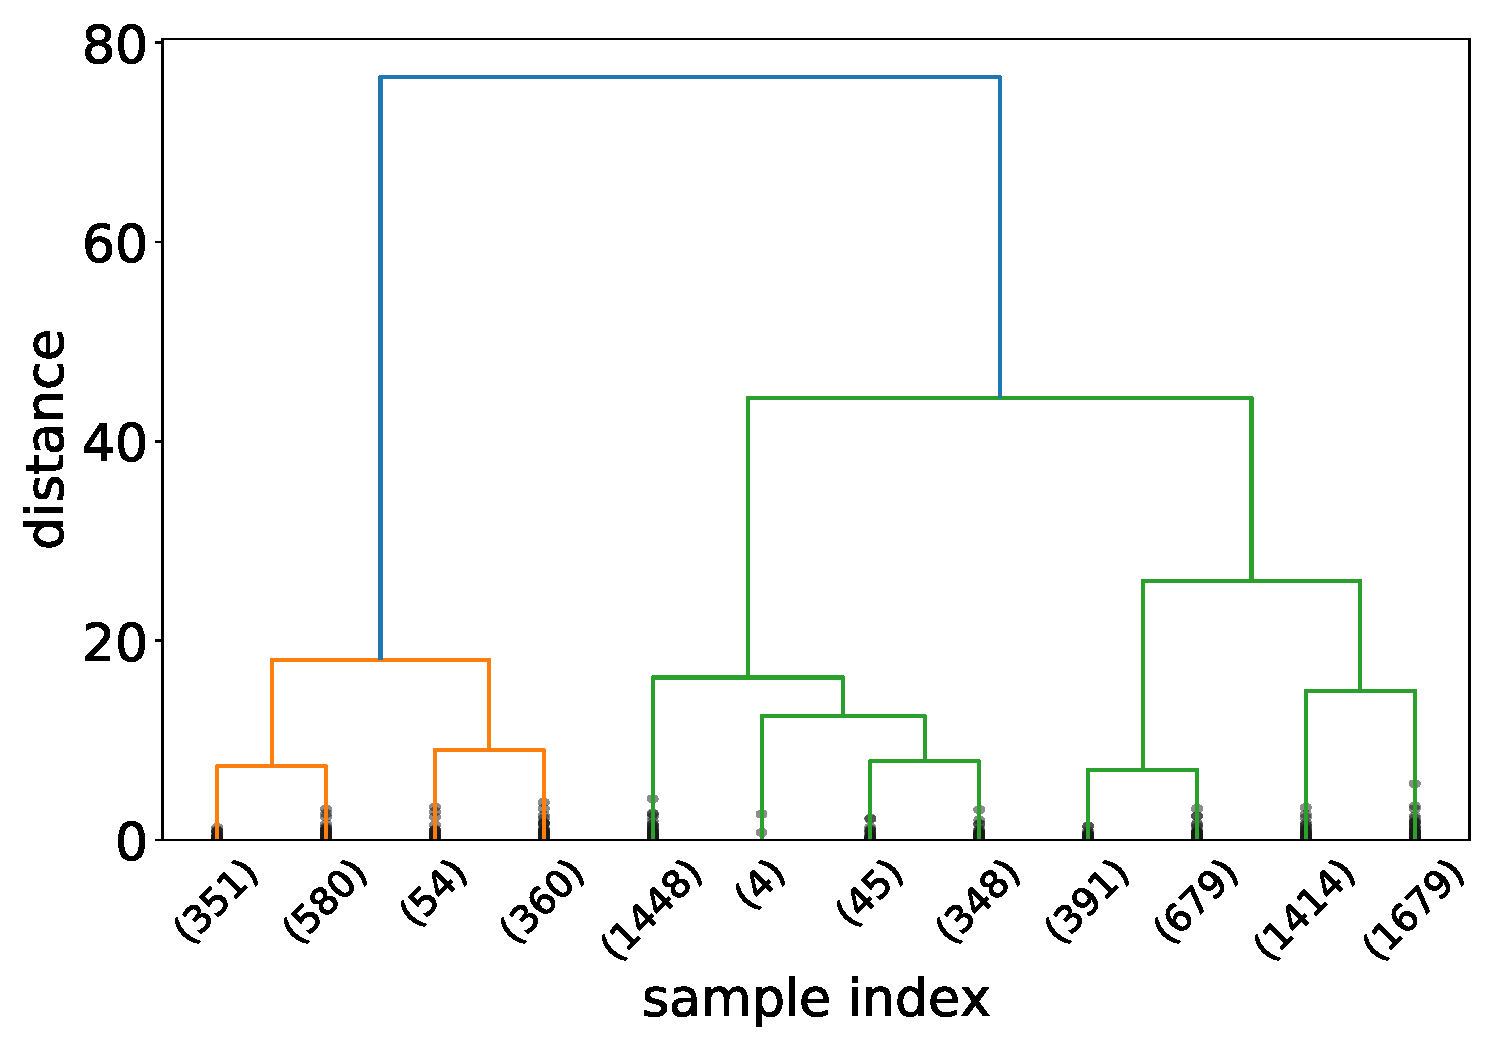
\includegraphics[width=0.9\linewidth]{Figs/Customer-Dendrograms.pdf}
    \caption{Costomer dendrogram...}
    \label{fig:dendrogram}
\end{figure}

\begin{figure}
	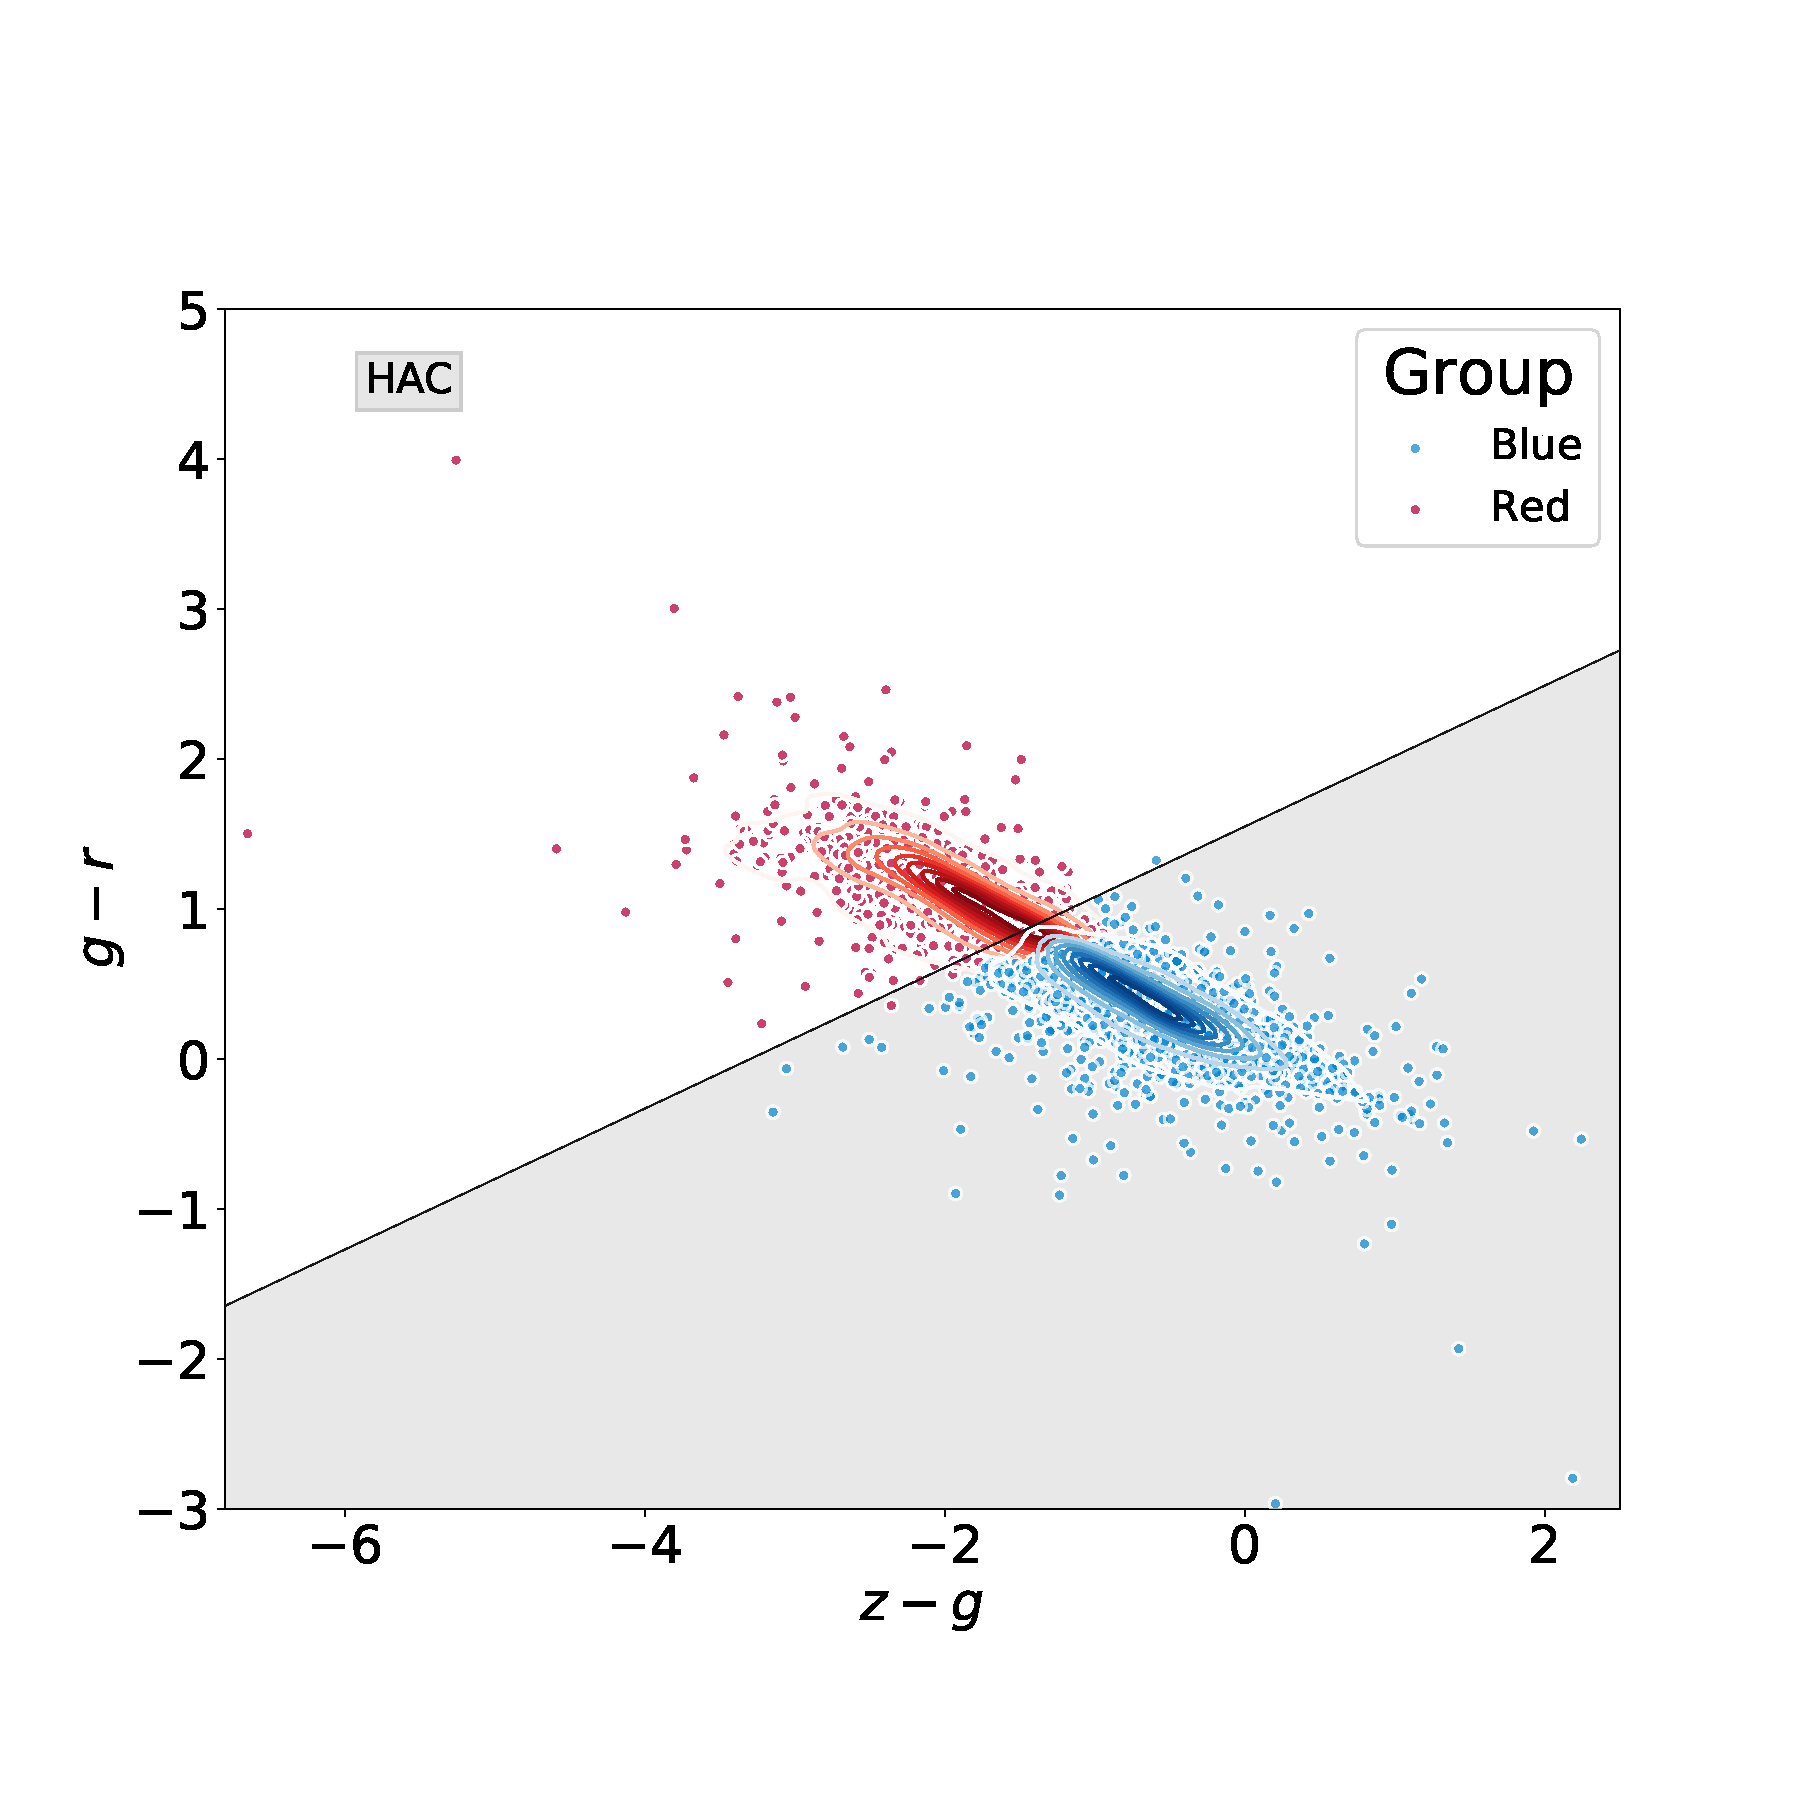
\includegraphics[width=0.9\linewidth]{Figs/blued-red-hierarchical.pdf}
    \caption{Costomer dendrogram...}
    \label{fig:hierar}
\end{figure}

\begin{figure*}
\centering
\begin{tabular}{l l}
  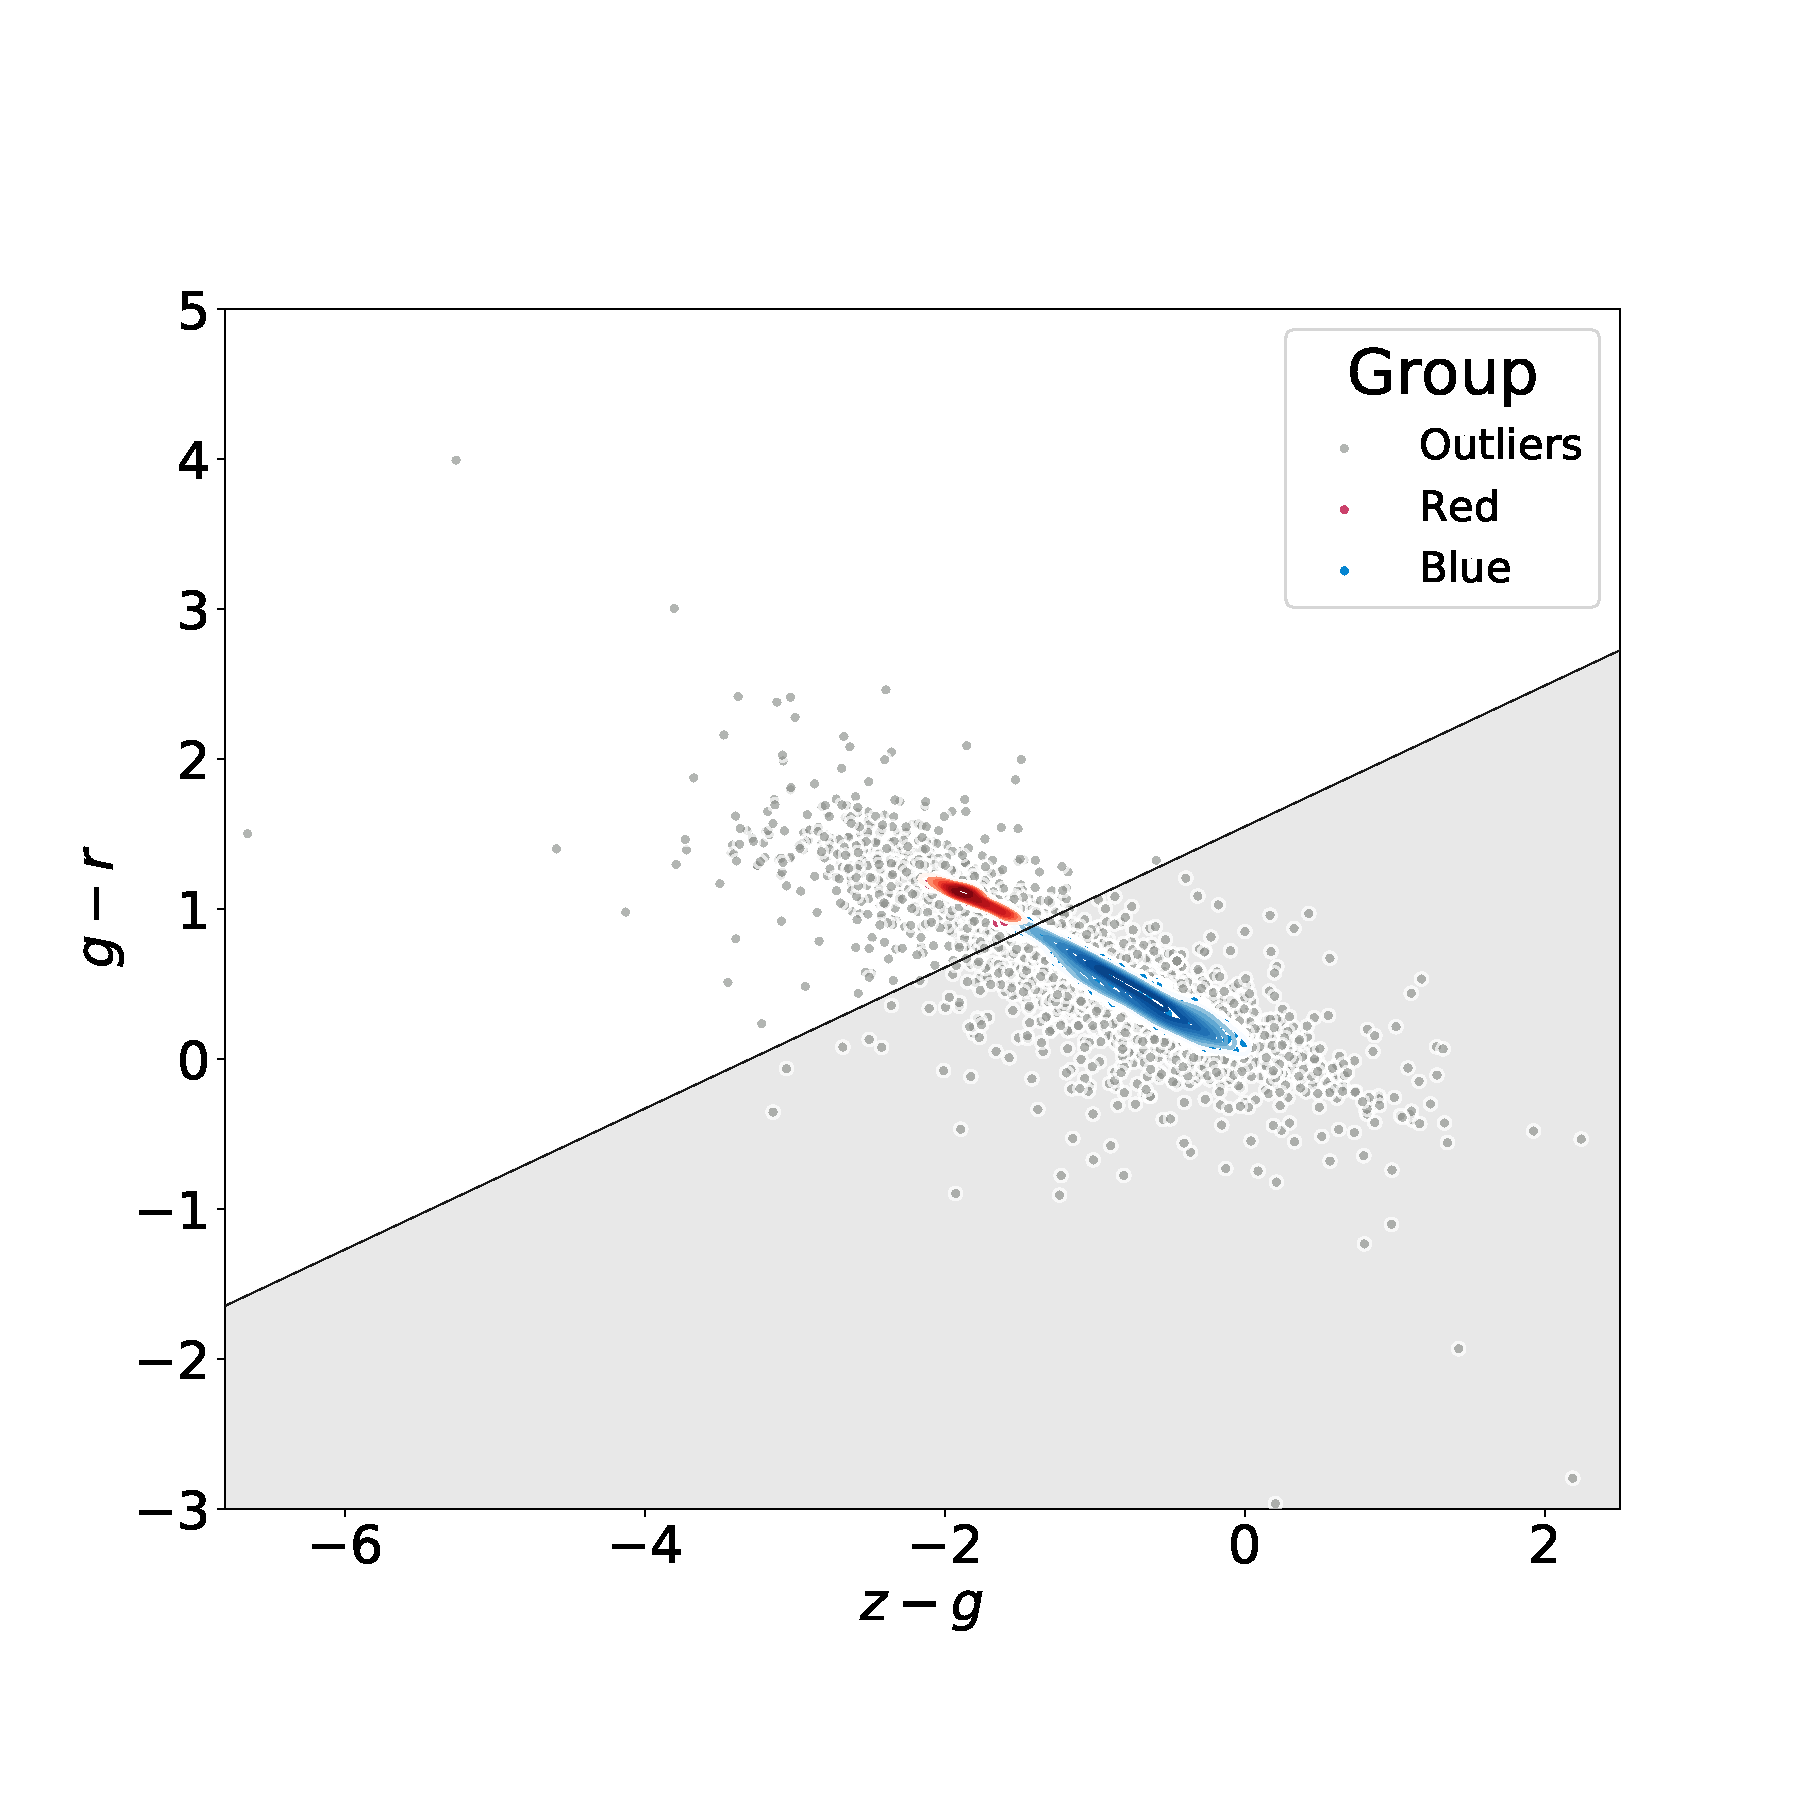
\includegraphics[width=0.5\linewidth, trim=10 10 5 8, clip]{Figs/blued-red-hdbscan.pdf}
   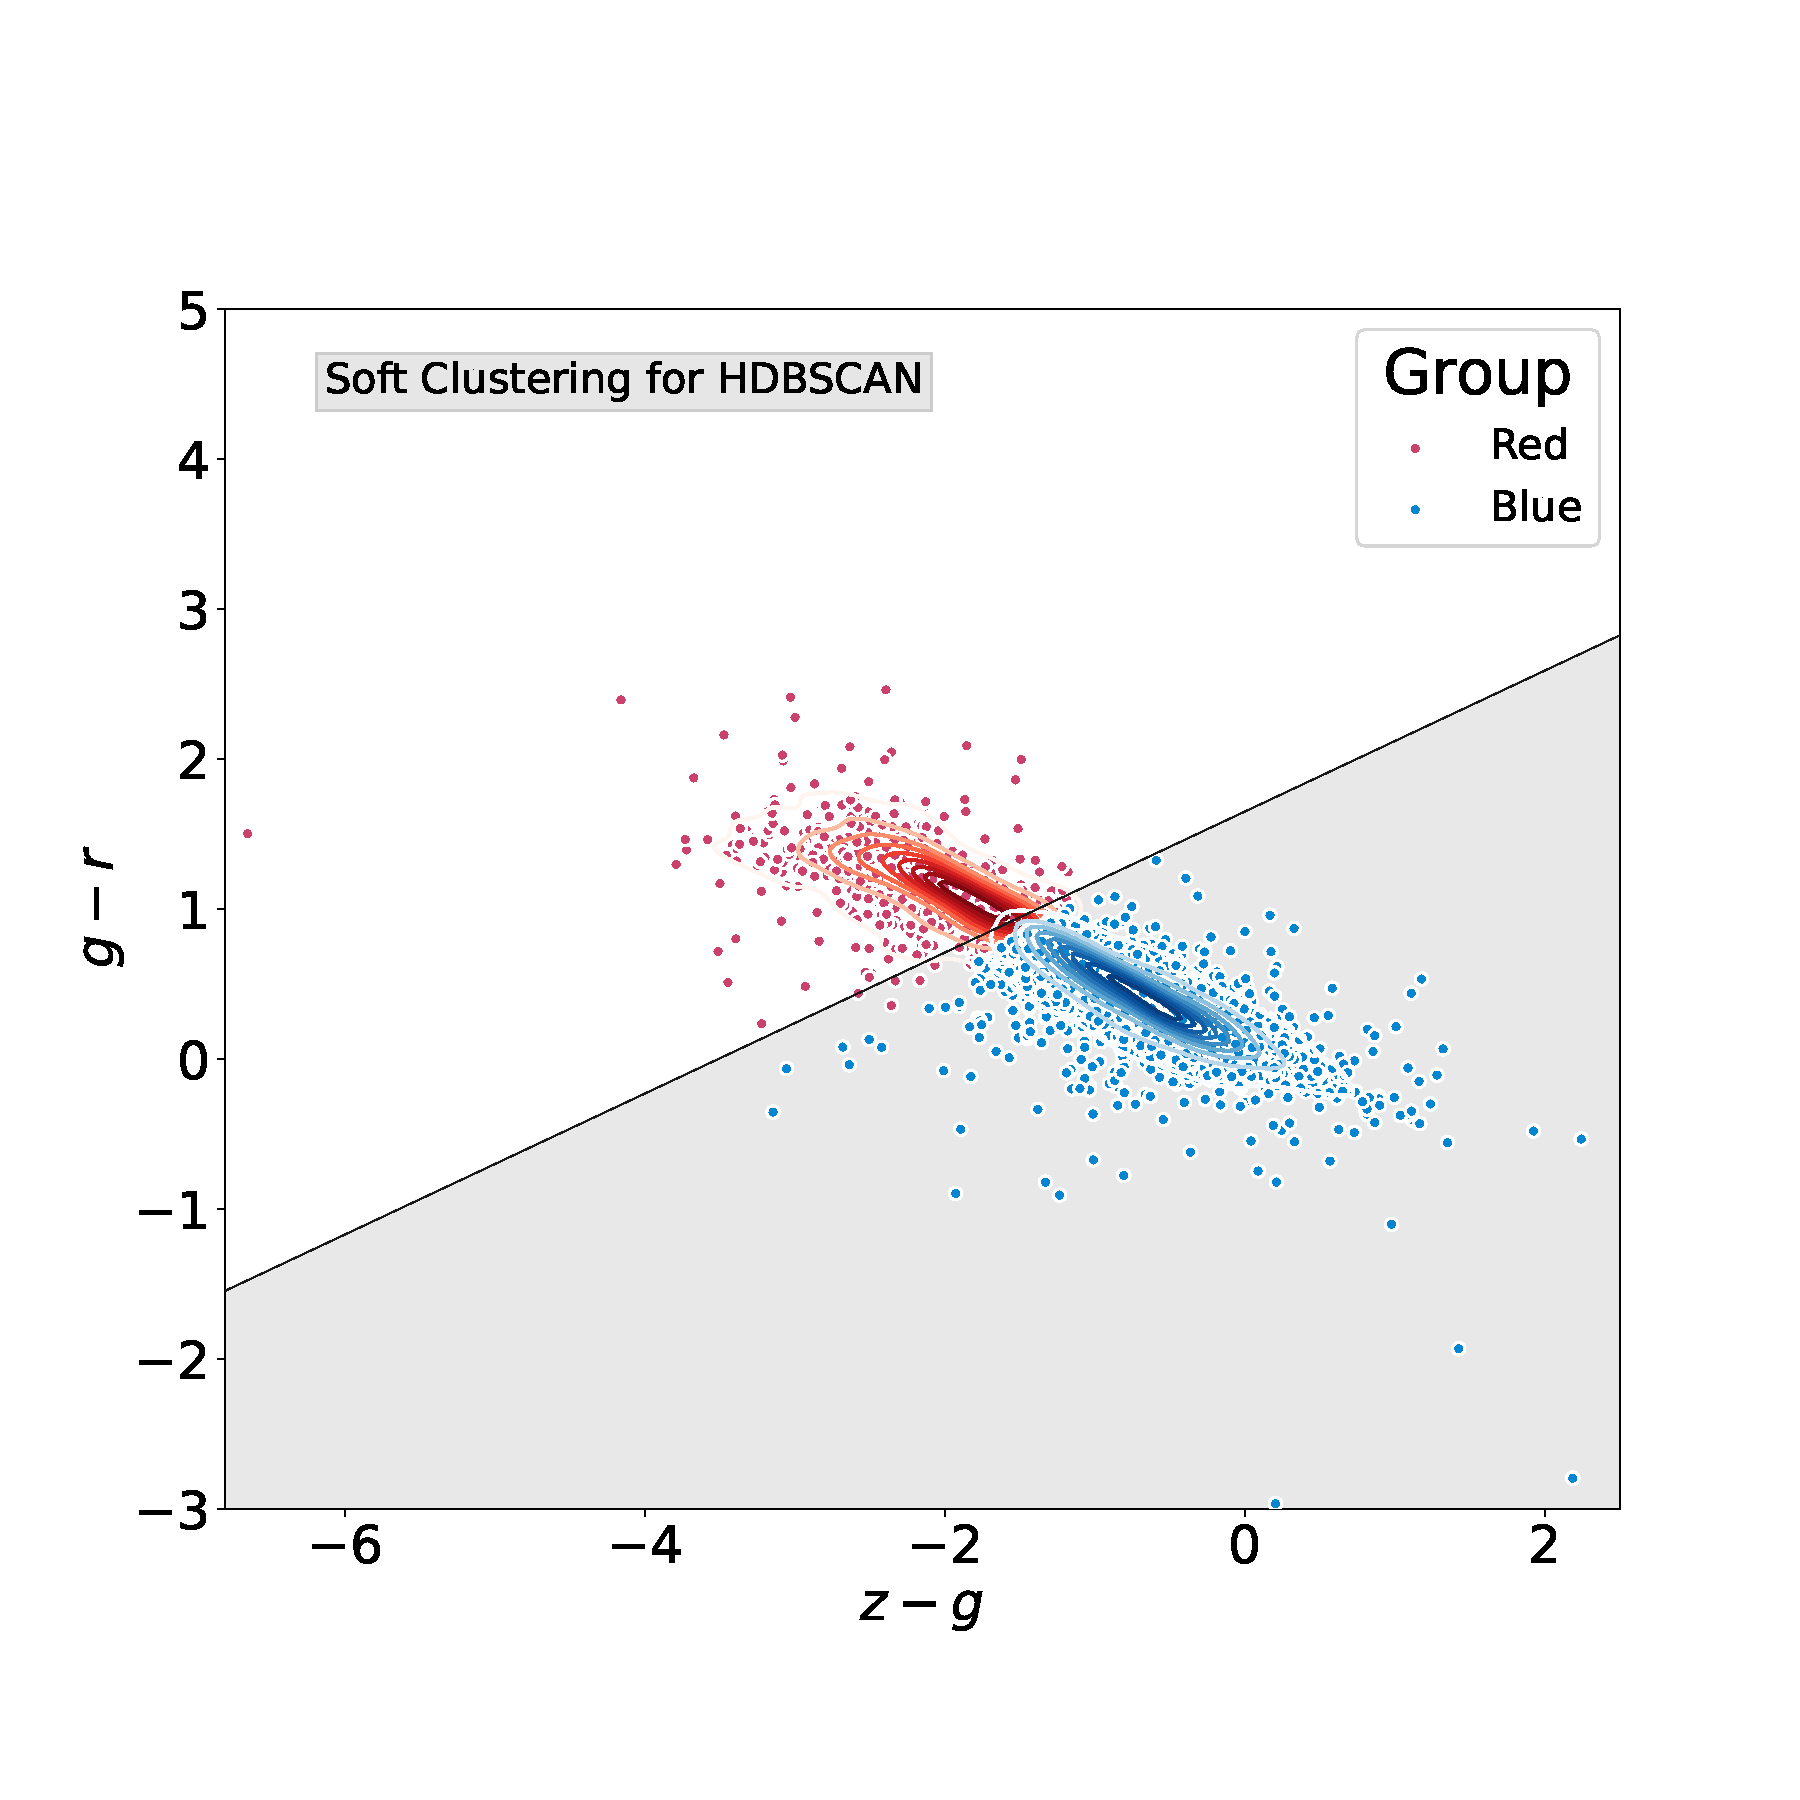
\includegraphics[width=0.5\linewidth, trim=10 10 5 8. clip]{Figs/blue-red-hdbscan-soft-alternative.pdf}
  \end{tabular}  
  \caption{New color-color diagram to separate the blue objects from the red ones.}
\label{fig:hdbscan}
\end{figure*}


\begin{figure*}
  \setlength\tabcolsep{0pt}
  \setkeys{Gin}{width=0.5\linewidth}
  \begin{tabular}{ll}
    (a) & (b) \\
    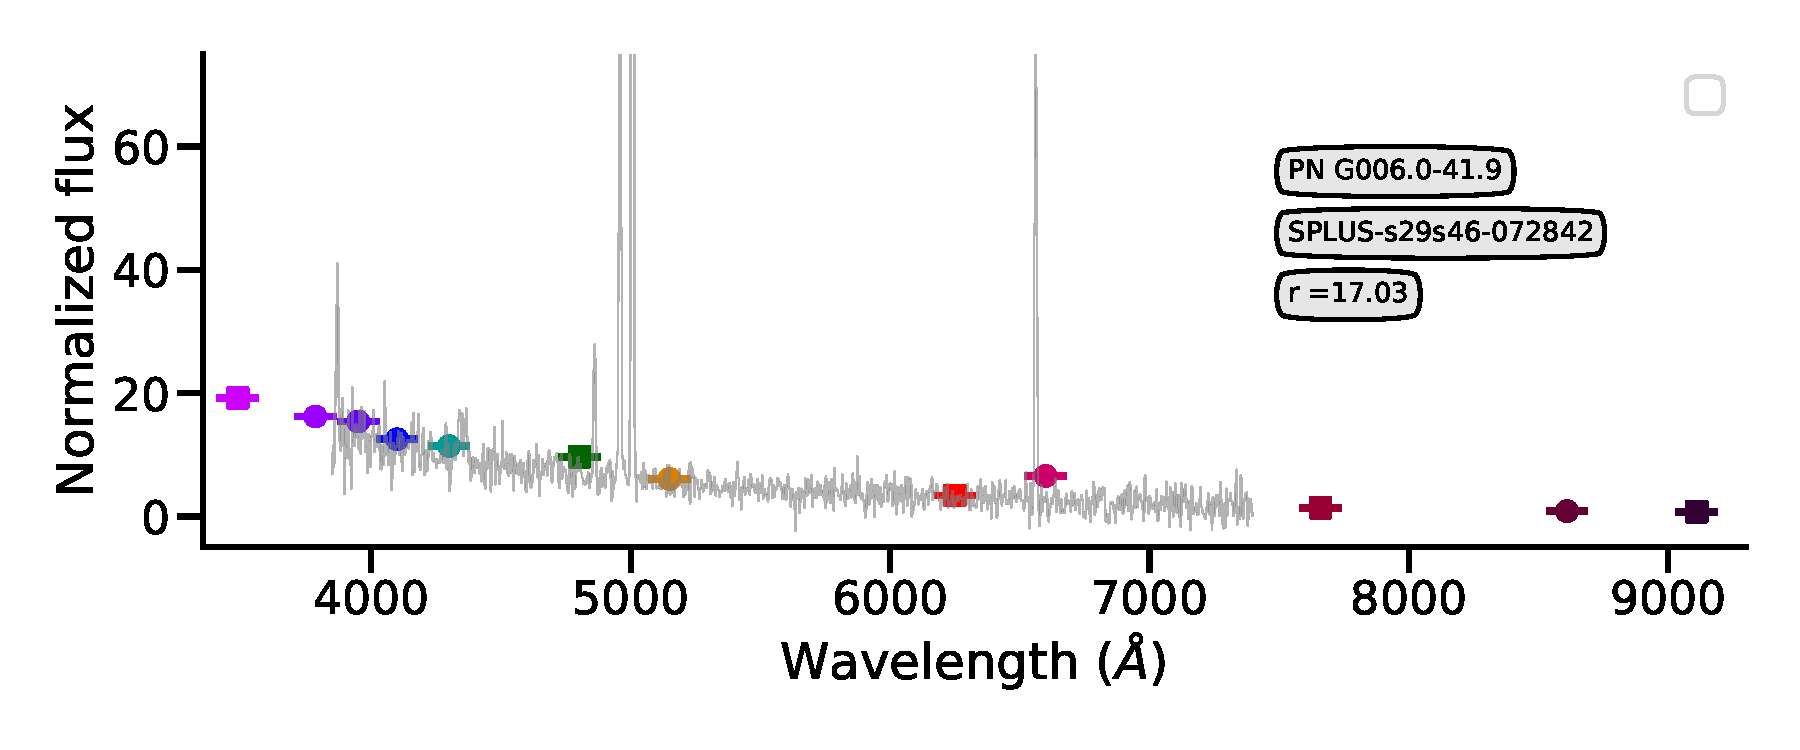
\includegraphics[trim=10 0 10 20, clip]{Figs/StenholmAcker_pn_g006_0-41_9_id176-SPLUS-s29s46-072842.pdf}
    & 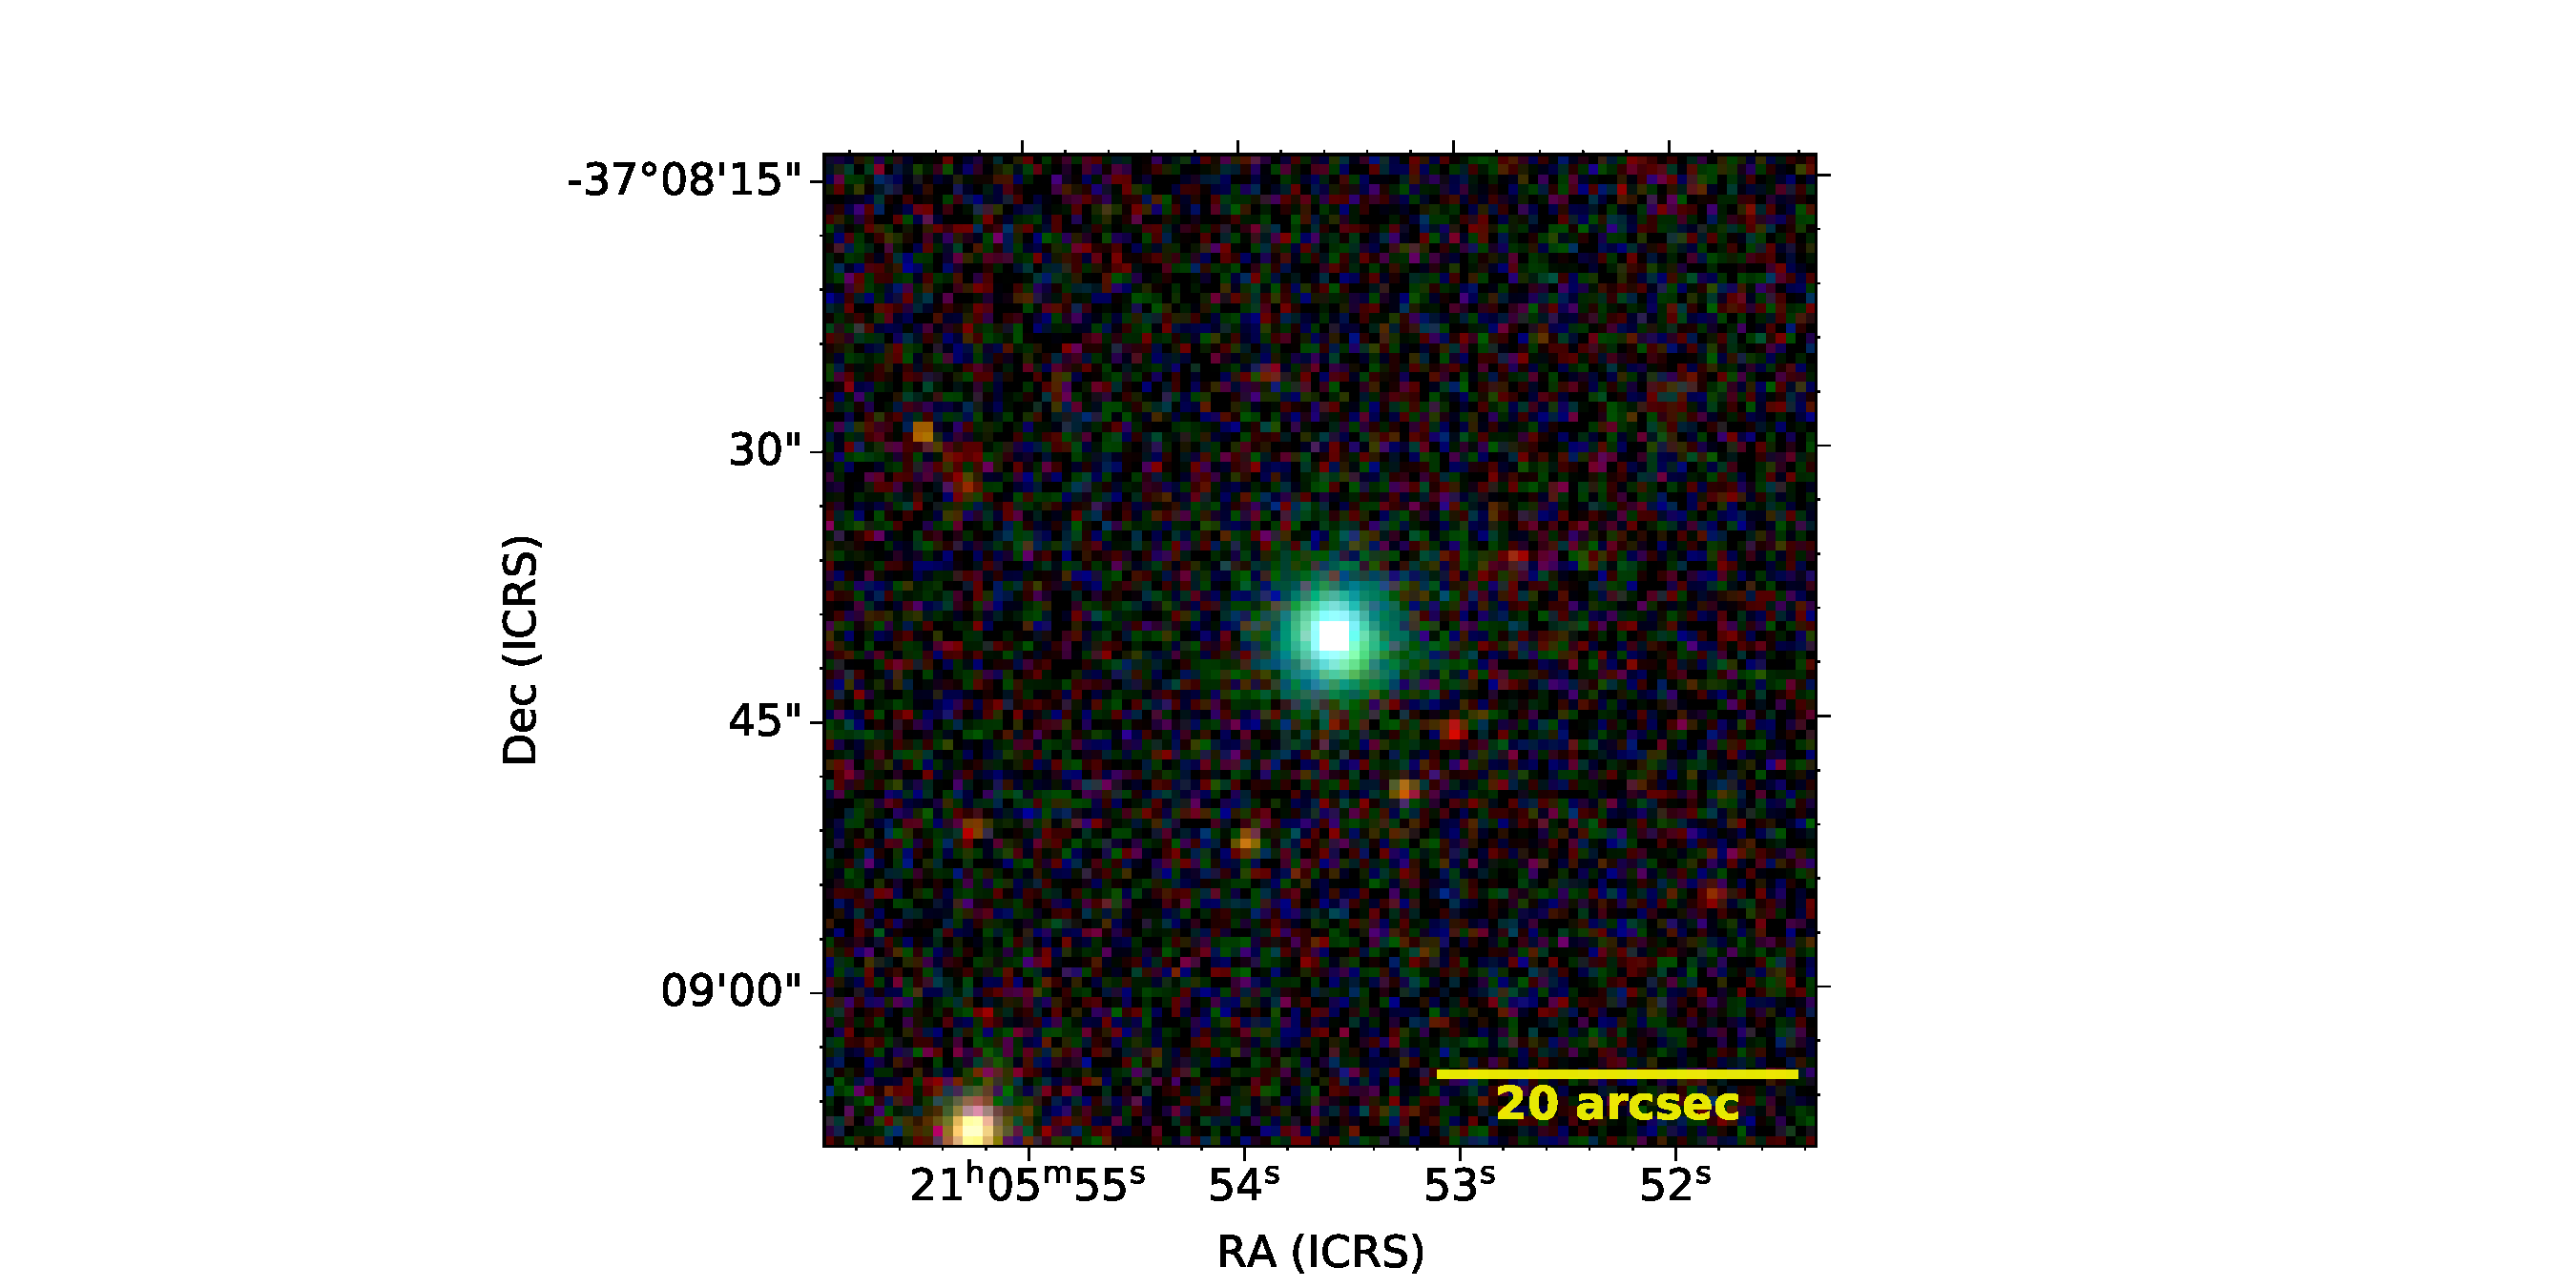
\includegraphics[width=0.4\linewidth, trim=10 0 10 20, clip]{Figs/PNG006_316-37_100_r.pdf} \\
    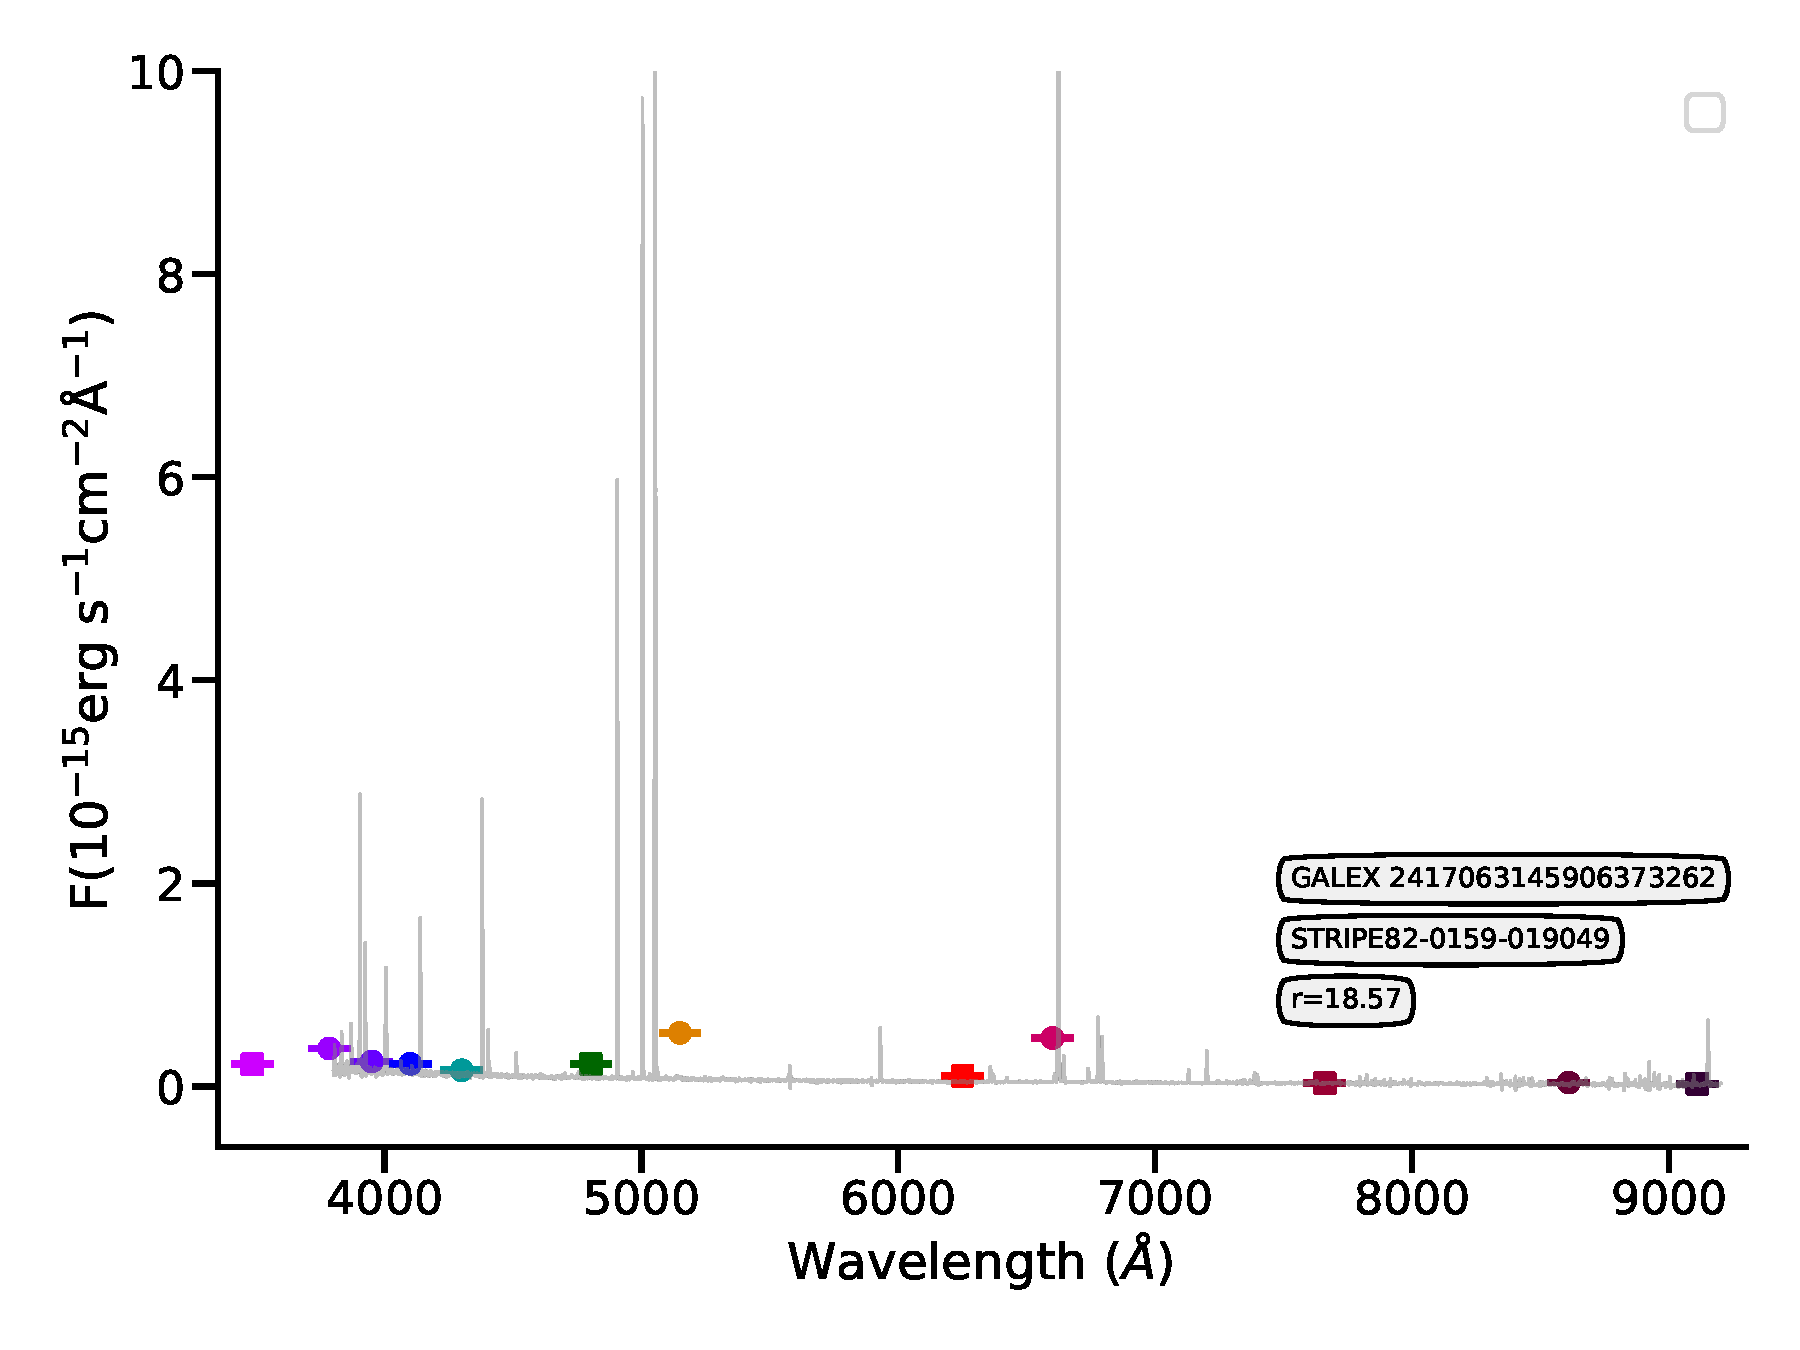
\includegraphics[trim=10 0 10 20, clip]{Figs/spec-0680-52200-0153-STRIPE82-0159-019049.pdf}
    & 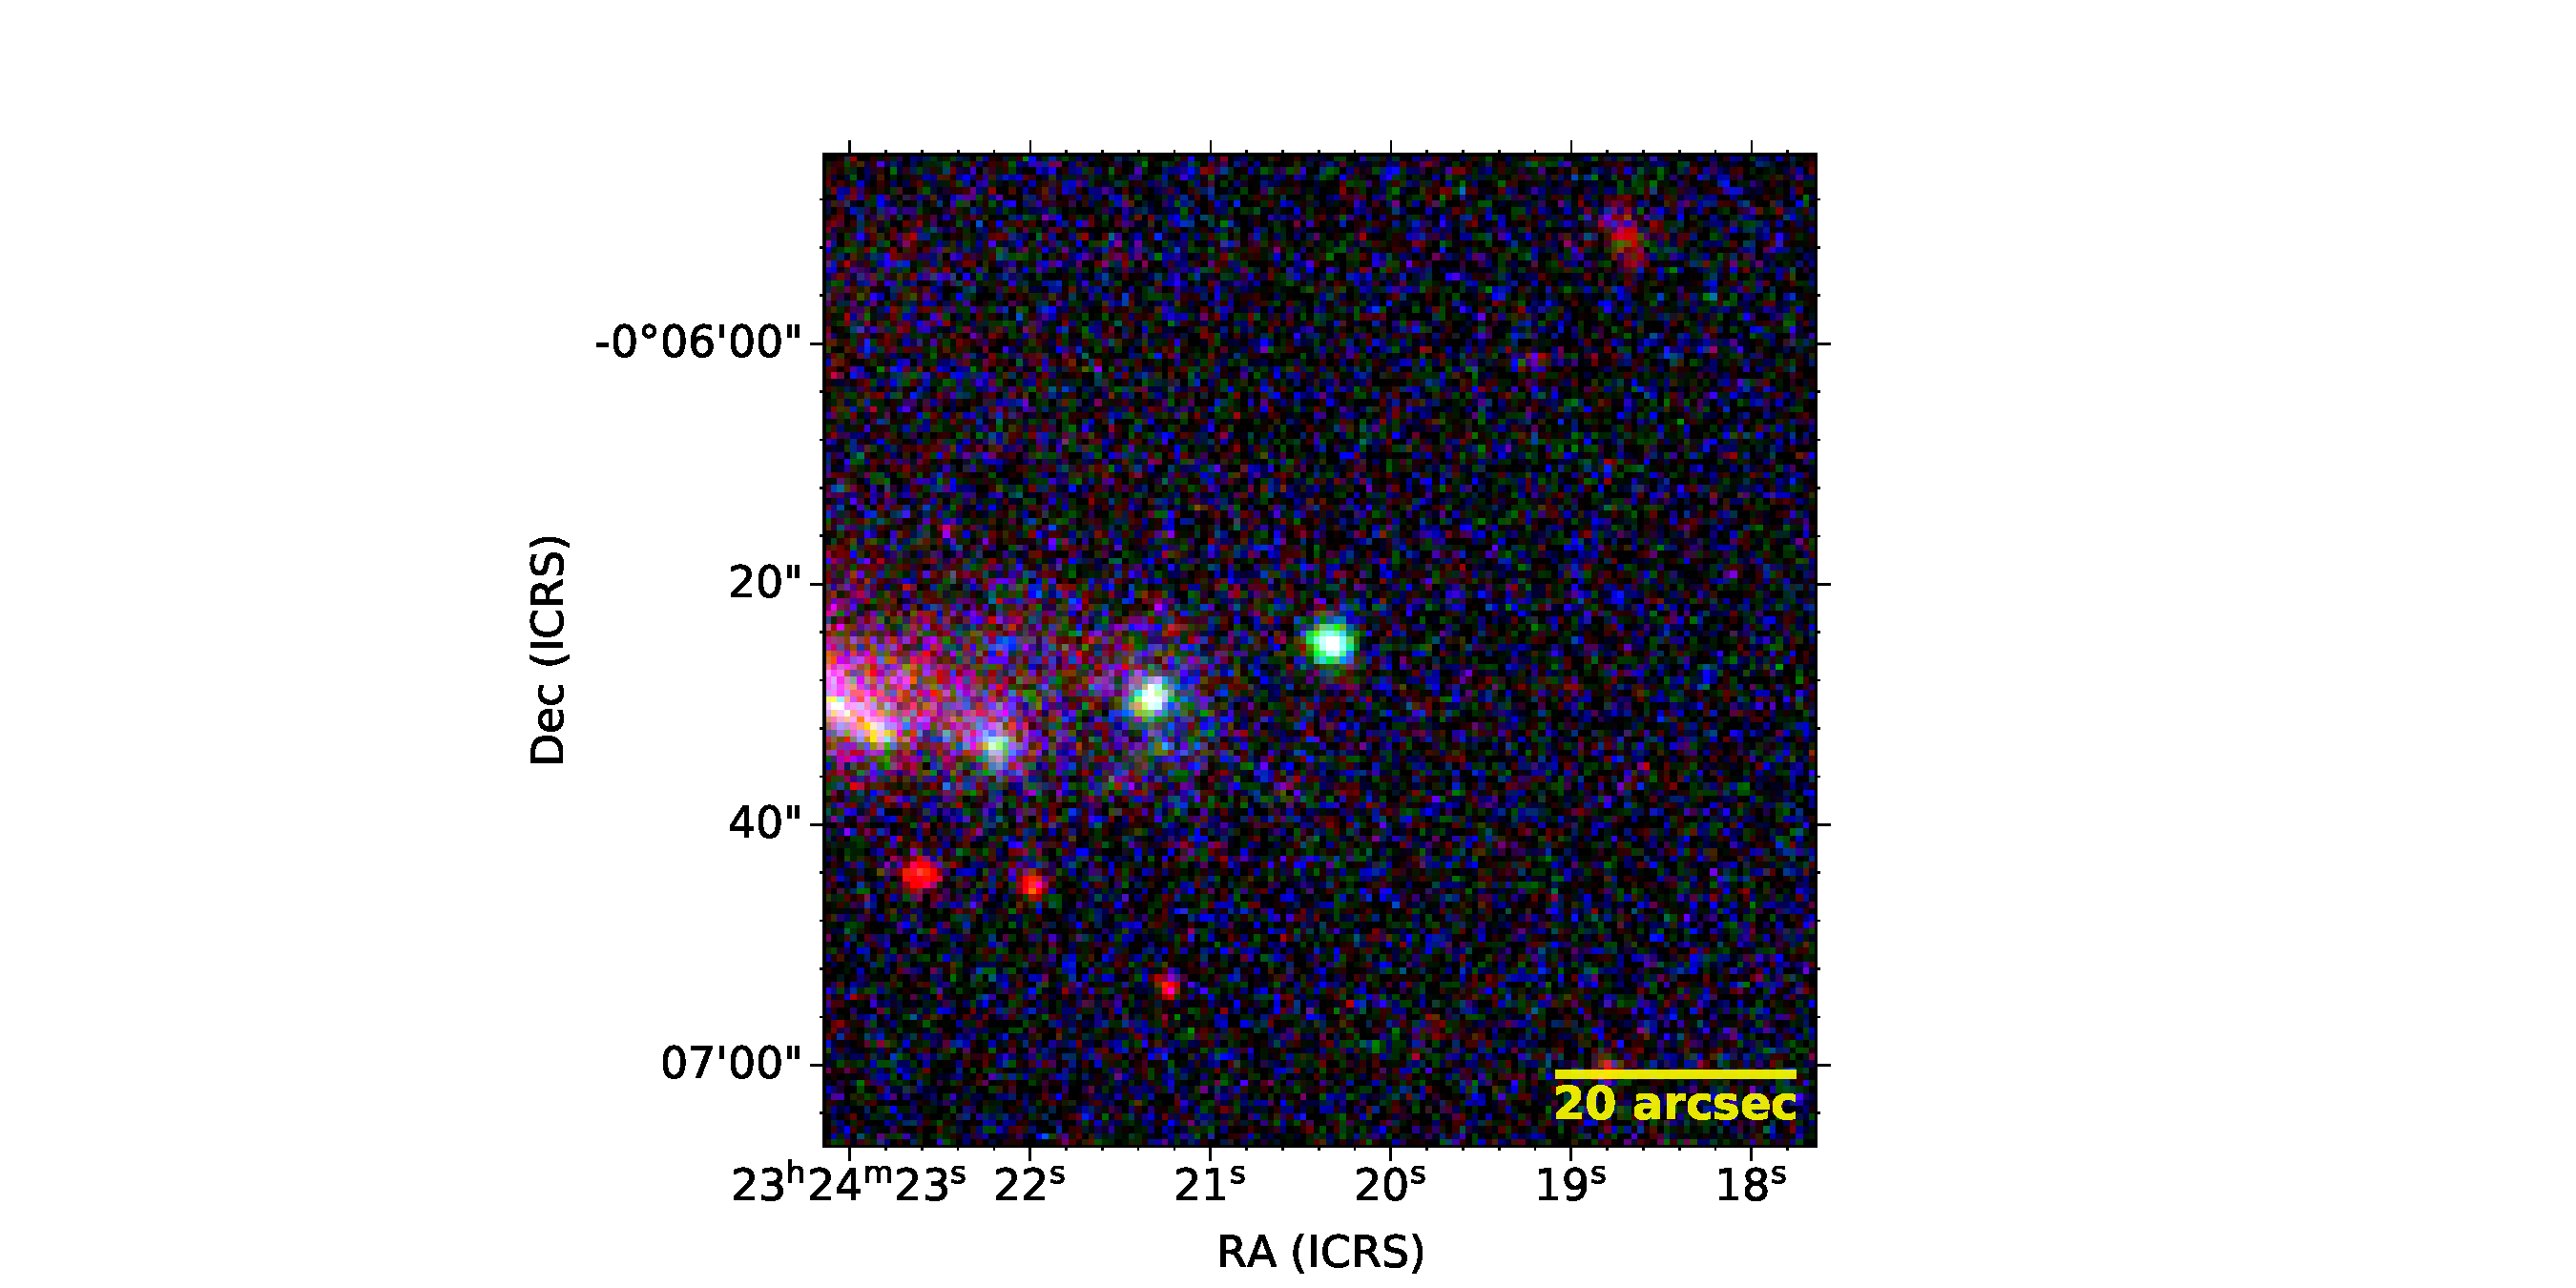
\includegraphics[width=0.4\linewidth, trim=10 0 10 20, clip]{Figs/GALEX24170_351-0_150_r.pdf} \\
    (c) & (d) \\
    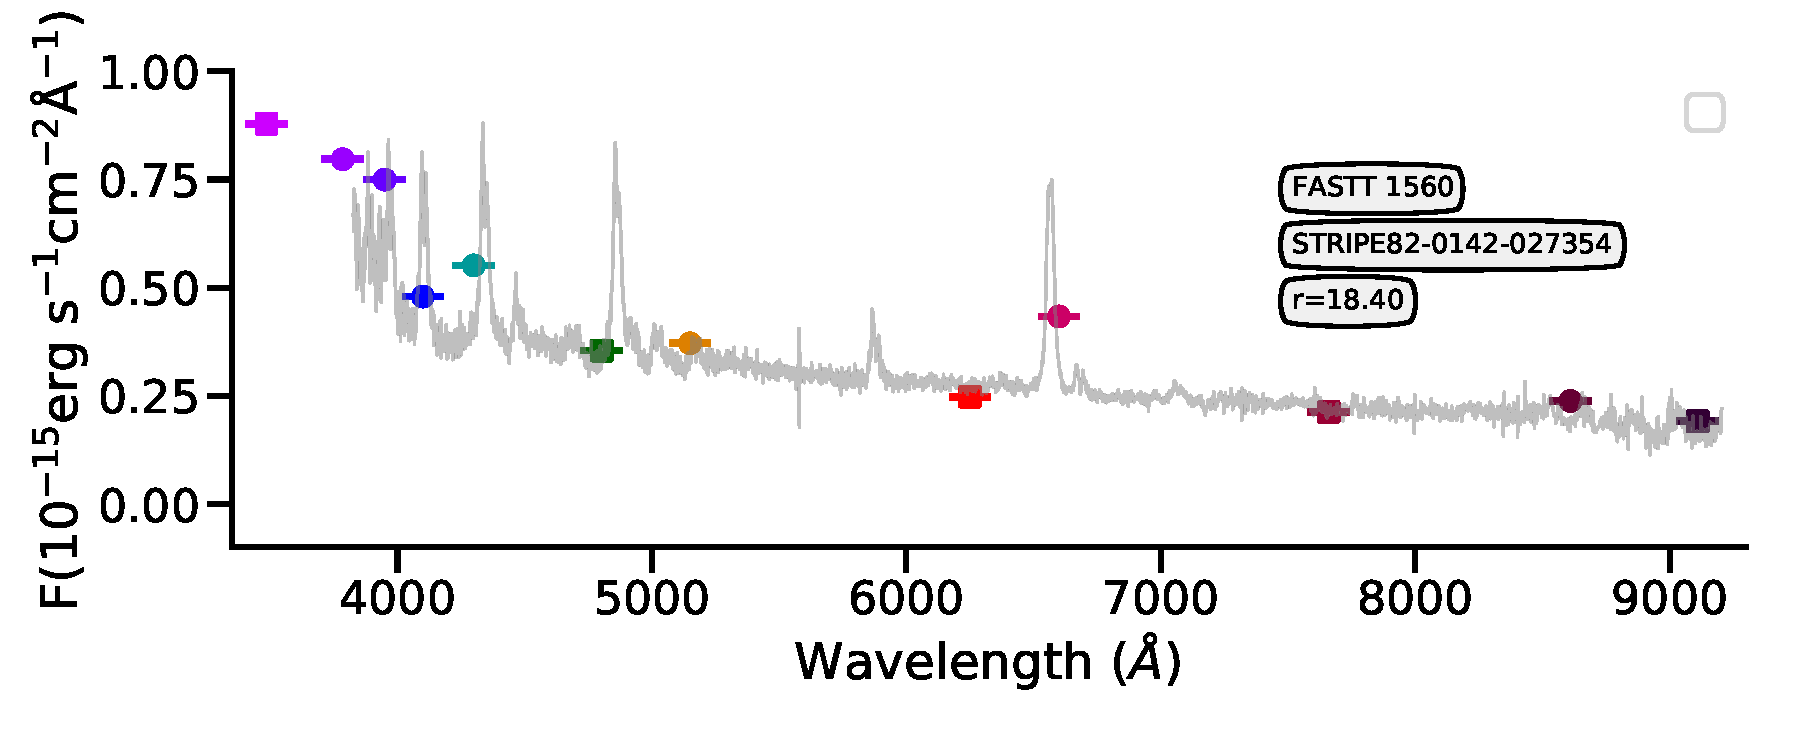
\includegraphics[trim=10 0 10 20, clip]{Figs/spec-0376-52143-0631-STRIPE82-0142-027354.pdf}
    & 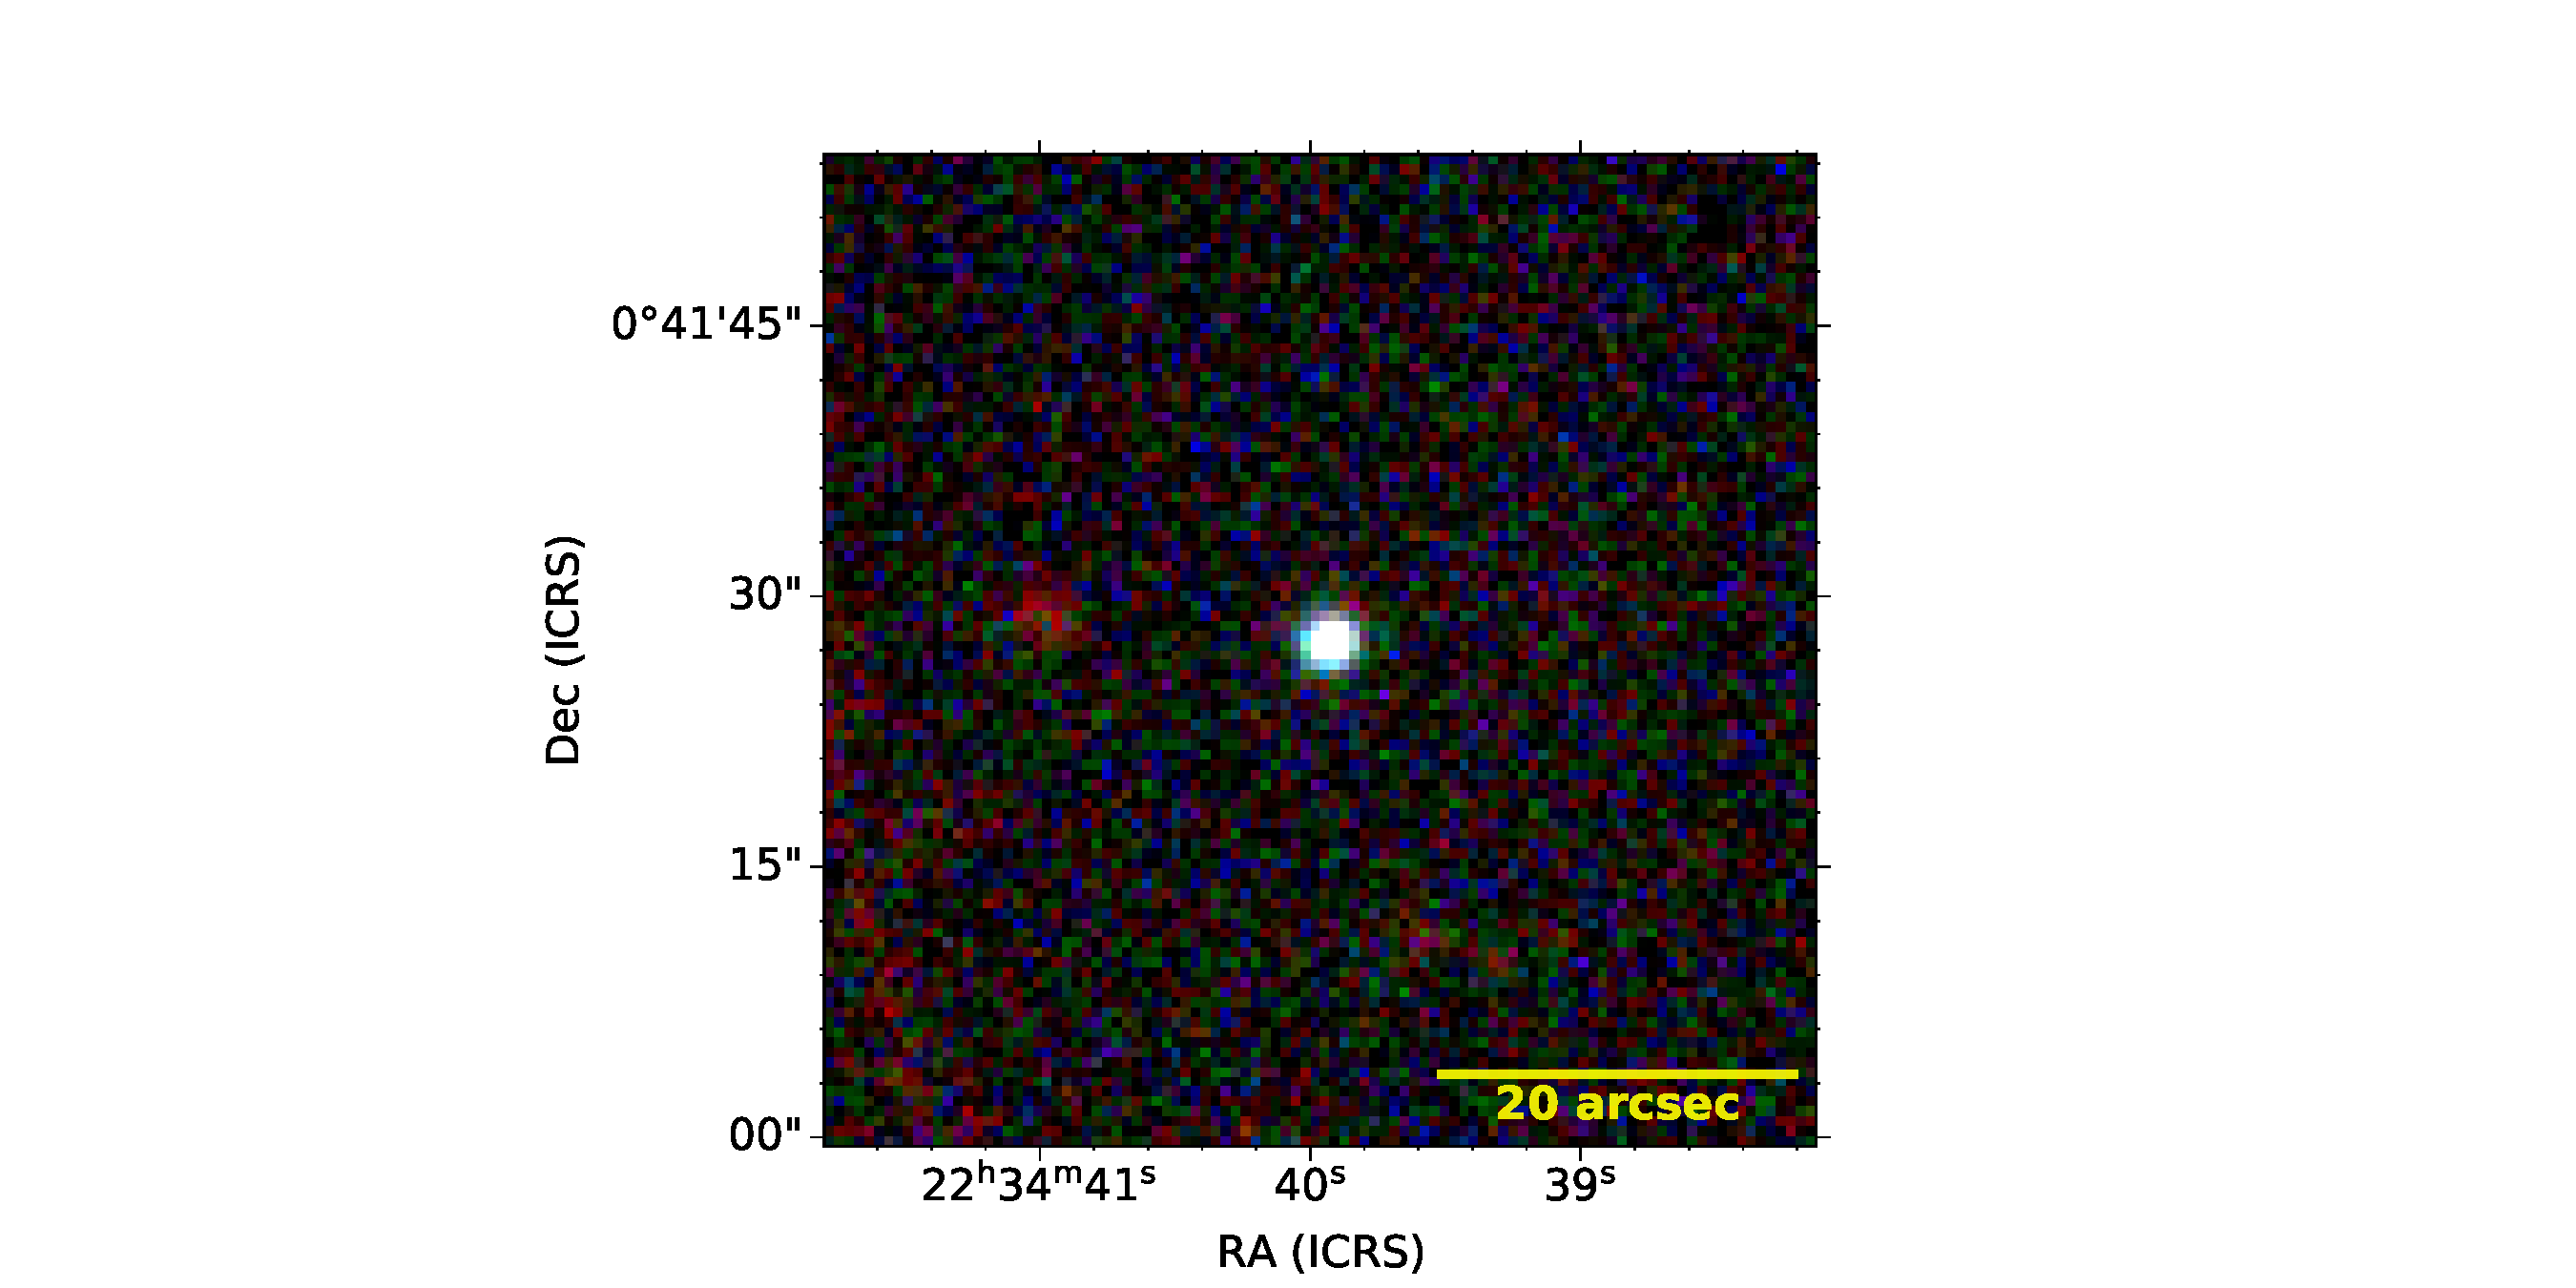
\includegraphics[width=0.4\linewidth, trim=10 0 10 20, clip]{Figs/FASTT1560_338-0_100_r.pdf} \\
    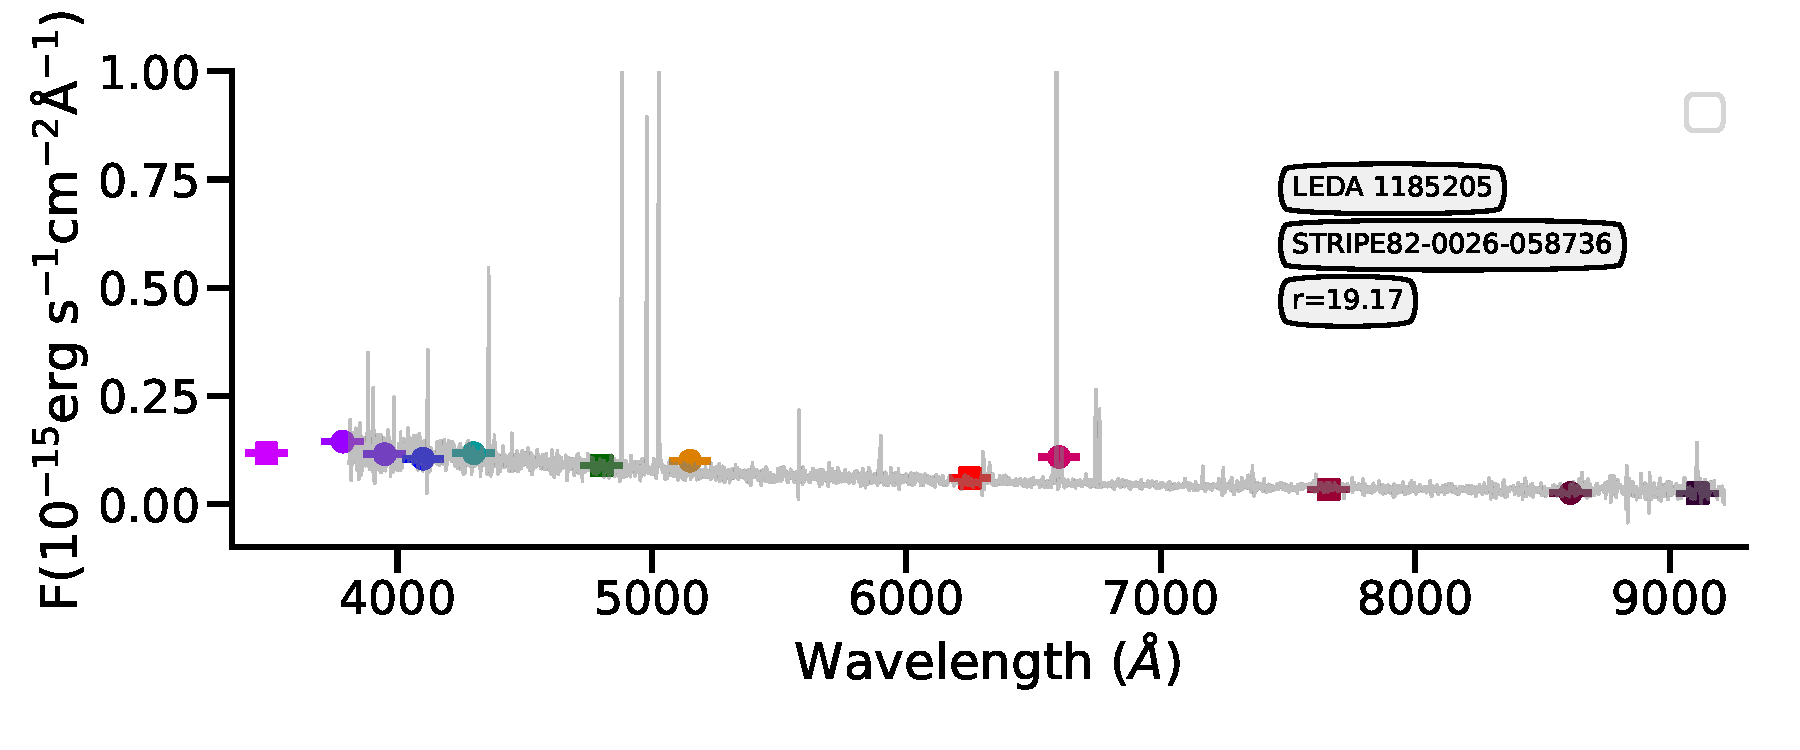
\includegraphics[trim=10 0 10 20, clip]{Figs/spec-0397-51794-0336-STRIPE82-0026-058736.pdf}
    & 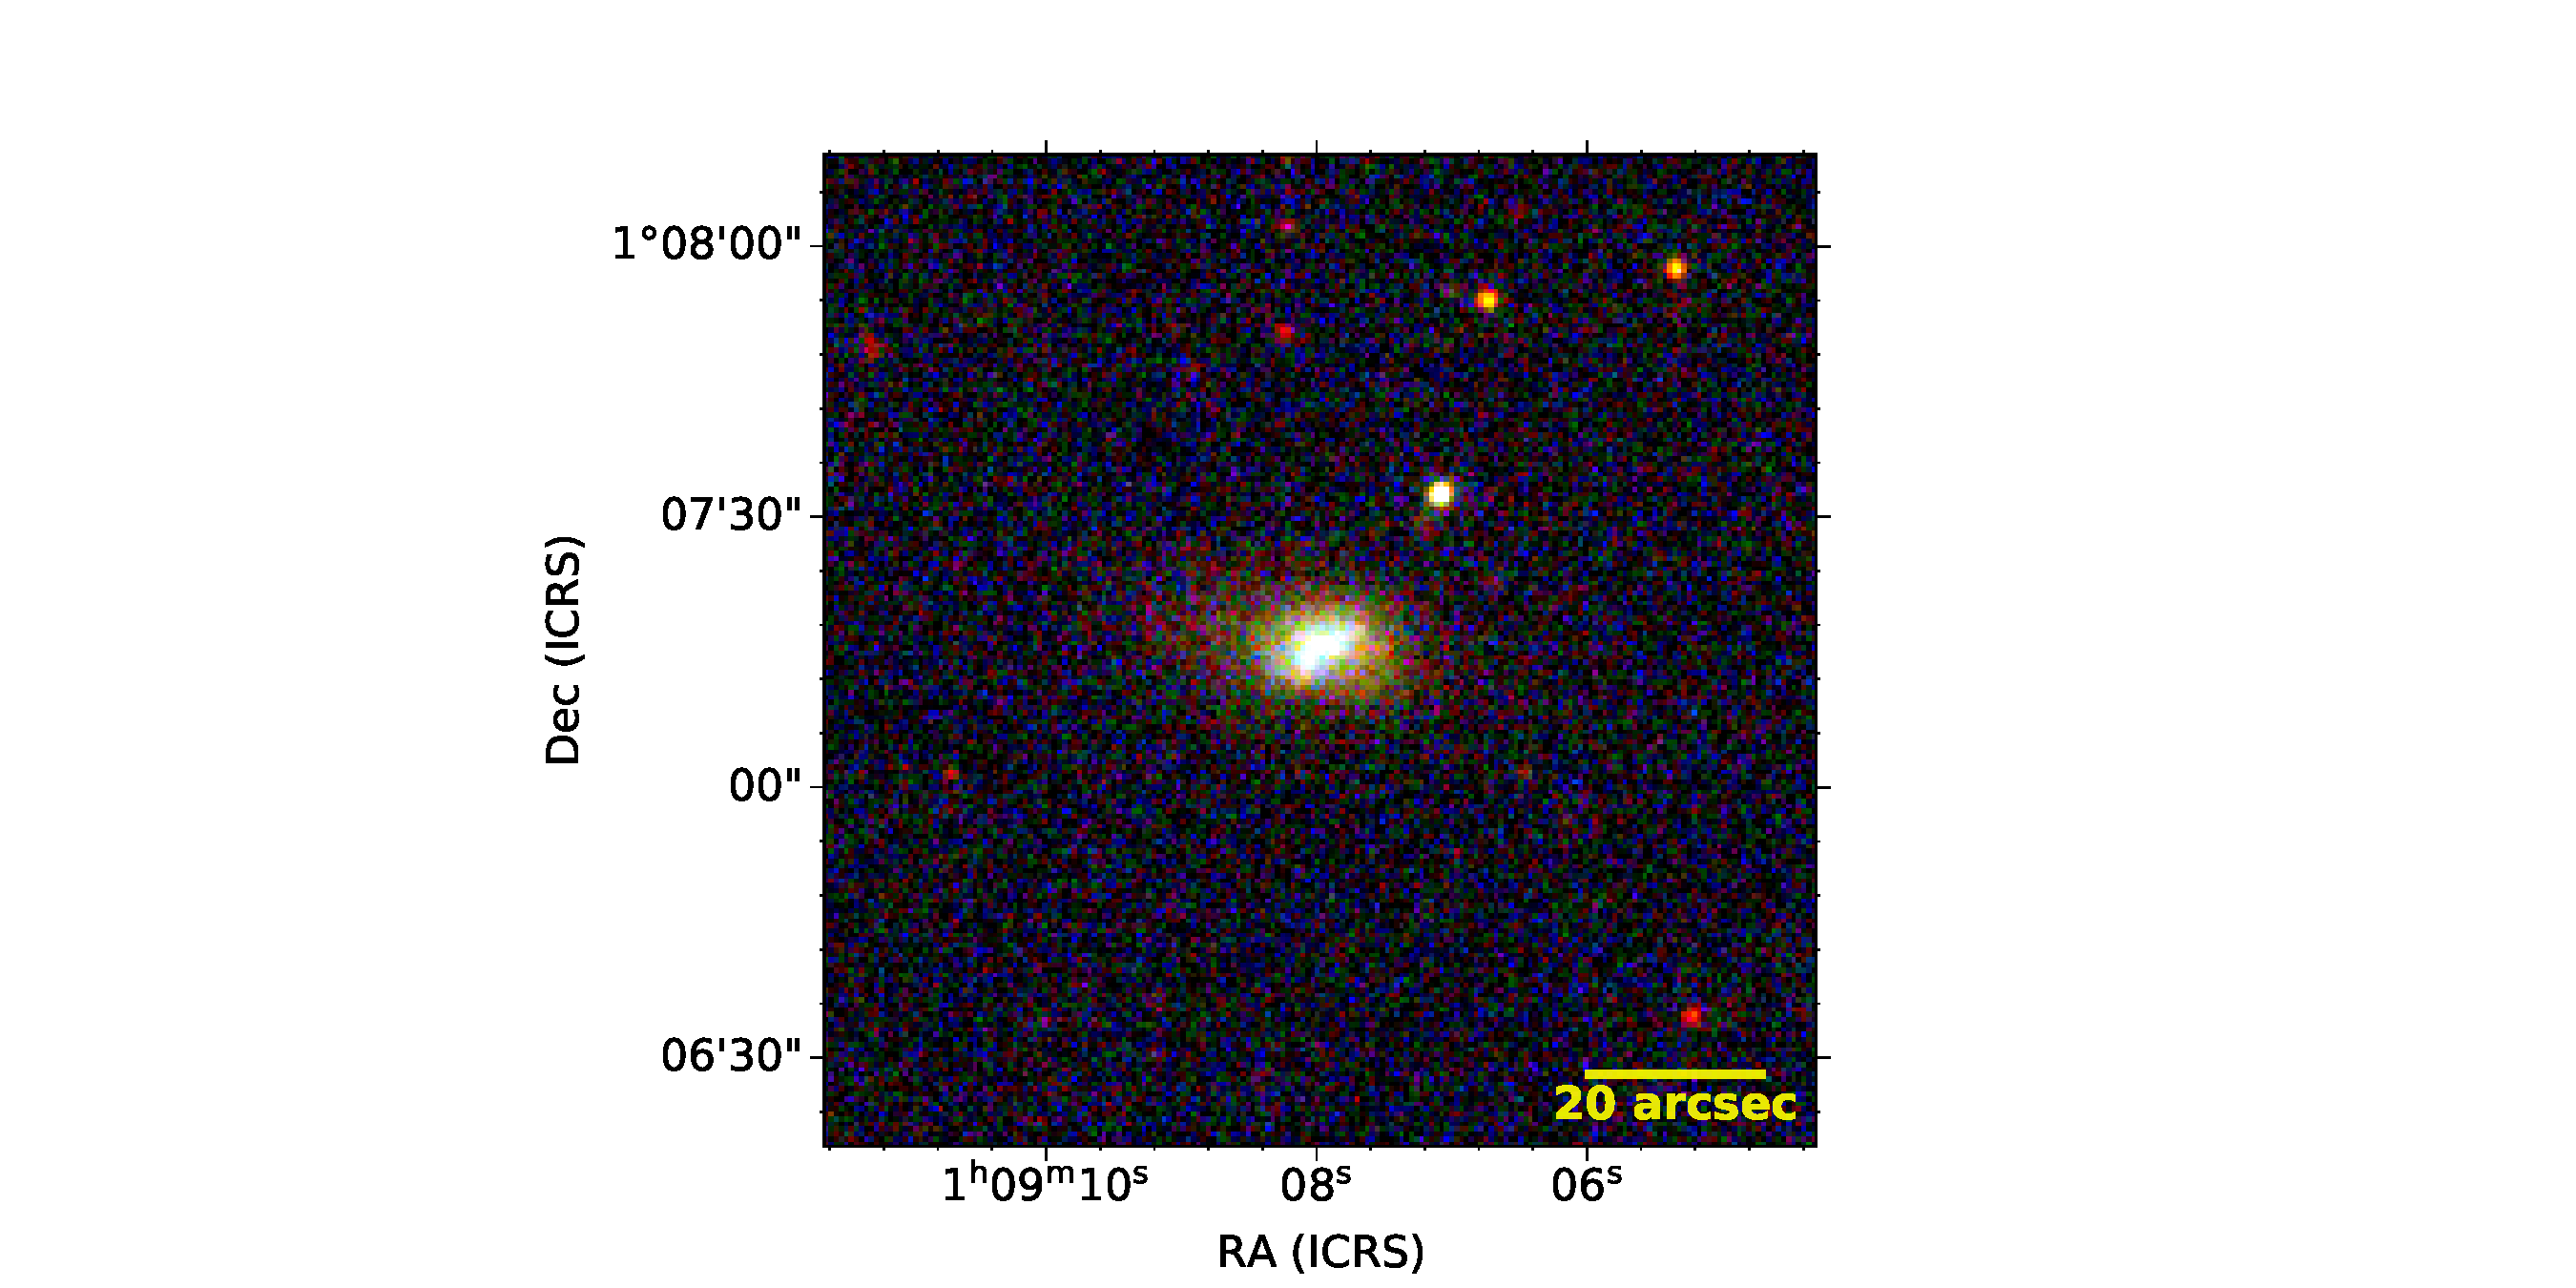
\includegraphics[width=0.4\linewidth, trim=10 0 10 20, clip]{Figs/LEDA1185205_17-1_200_r.pdf} \\
    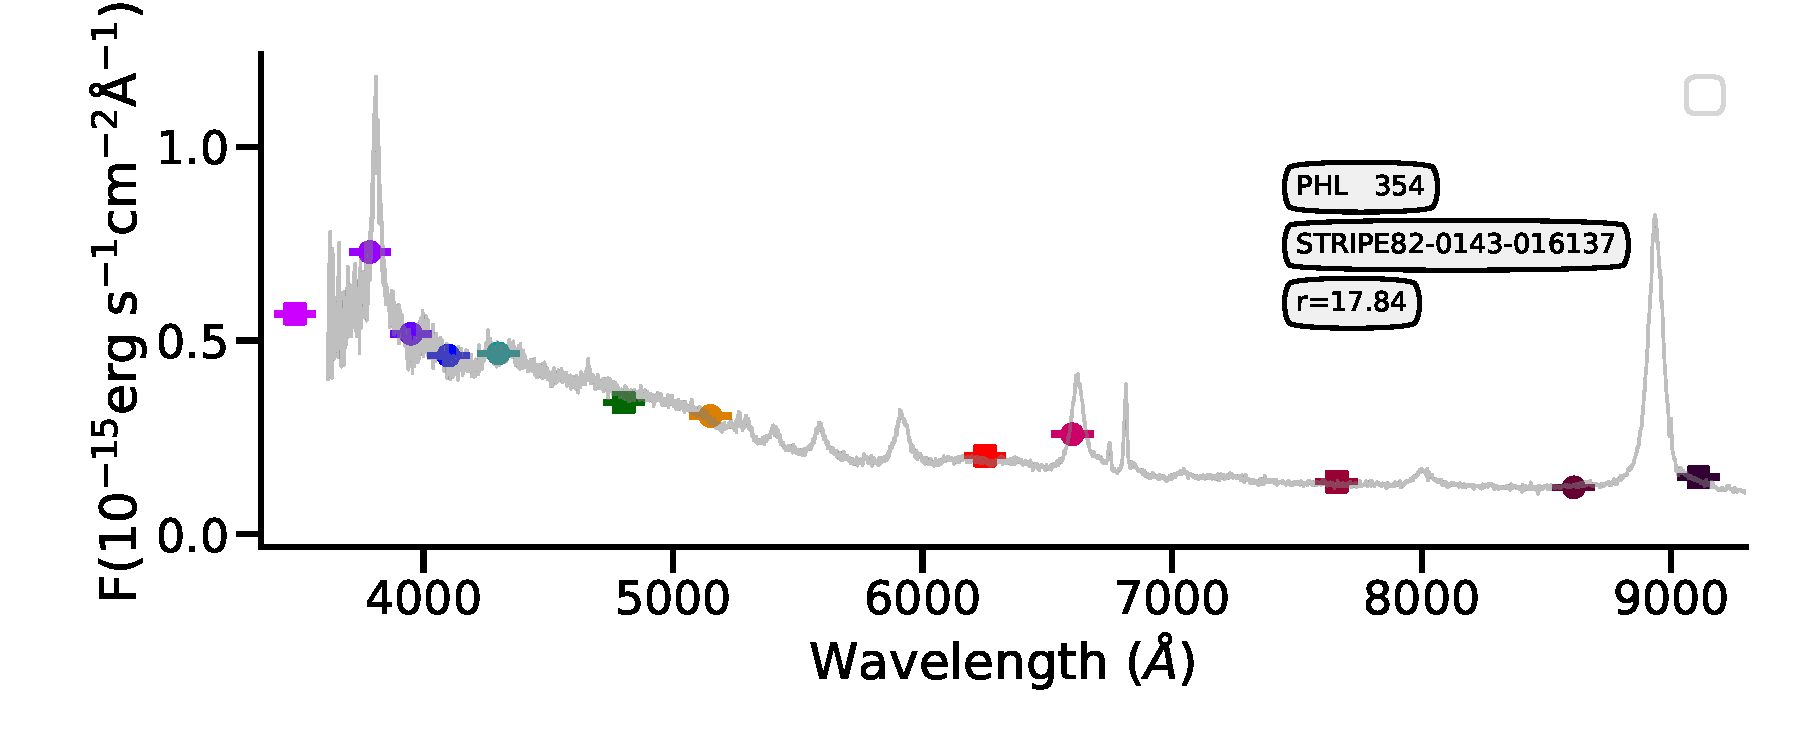
\includegraphics[trim=10 0 10 20, clip]{Figs/spec-9217-57934-0839-STRIPE82-0143-016137.pdf}
    & 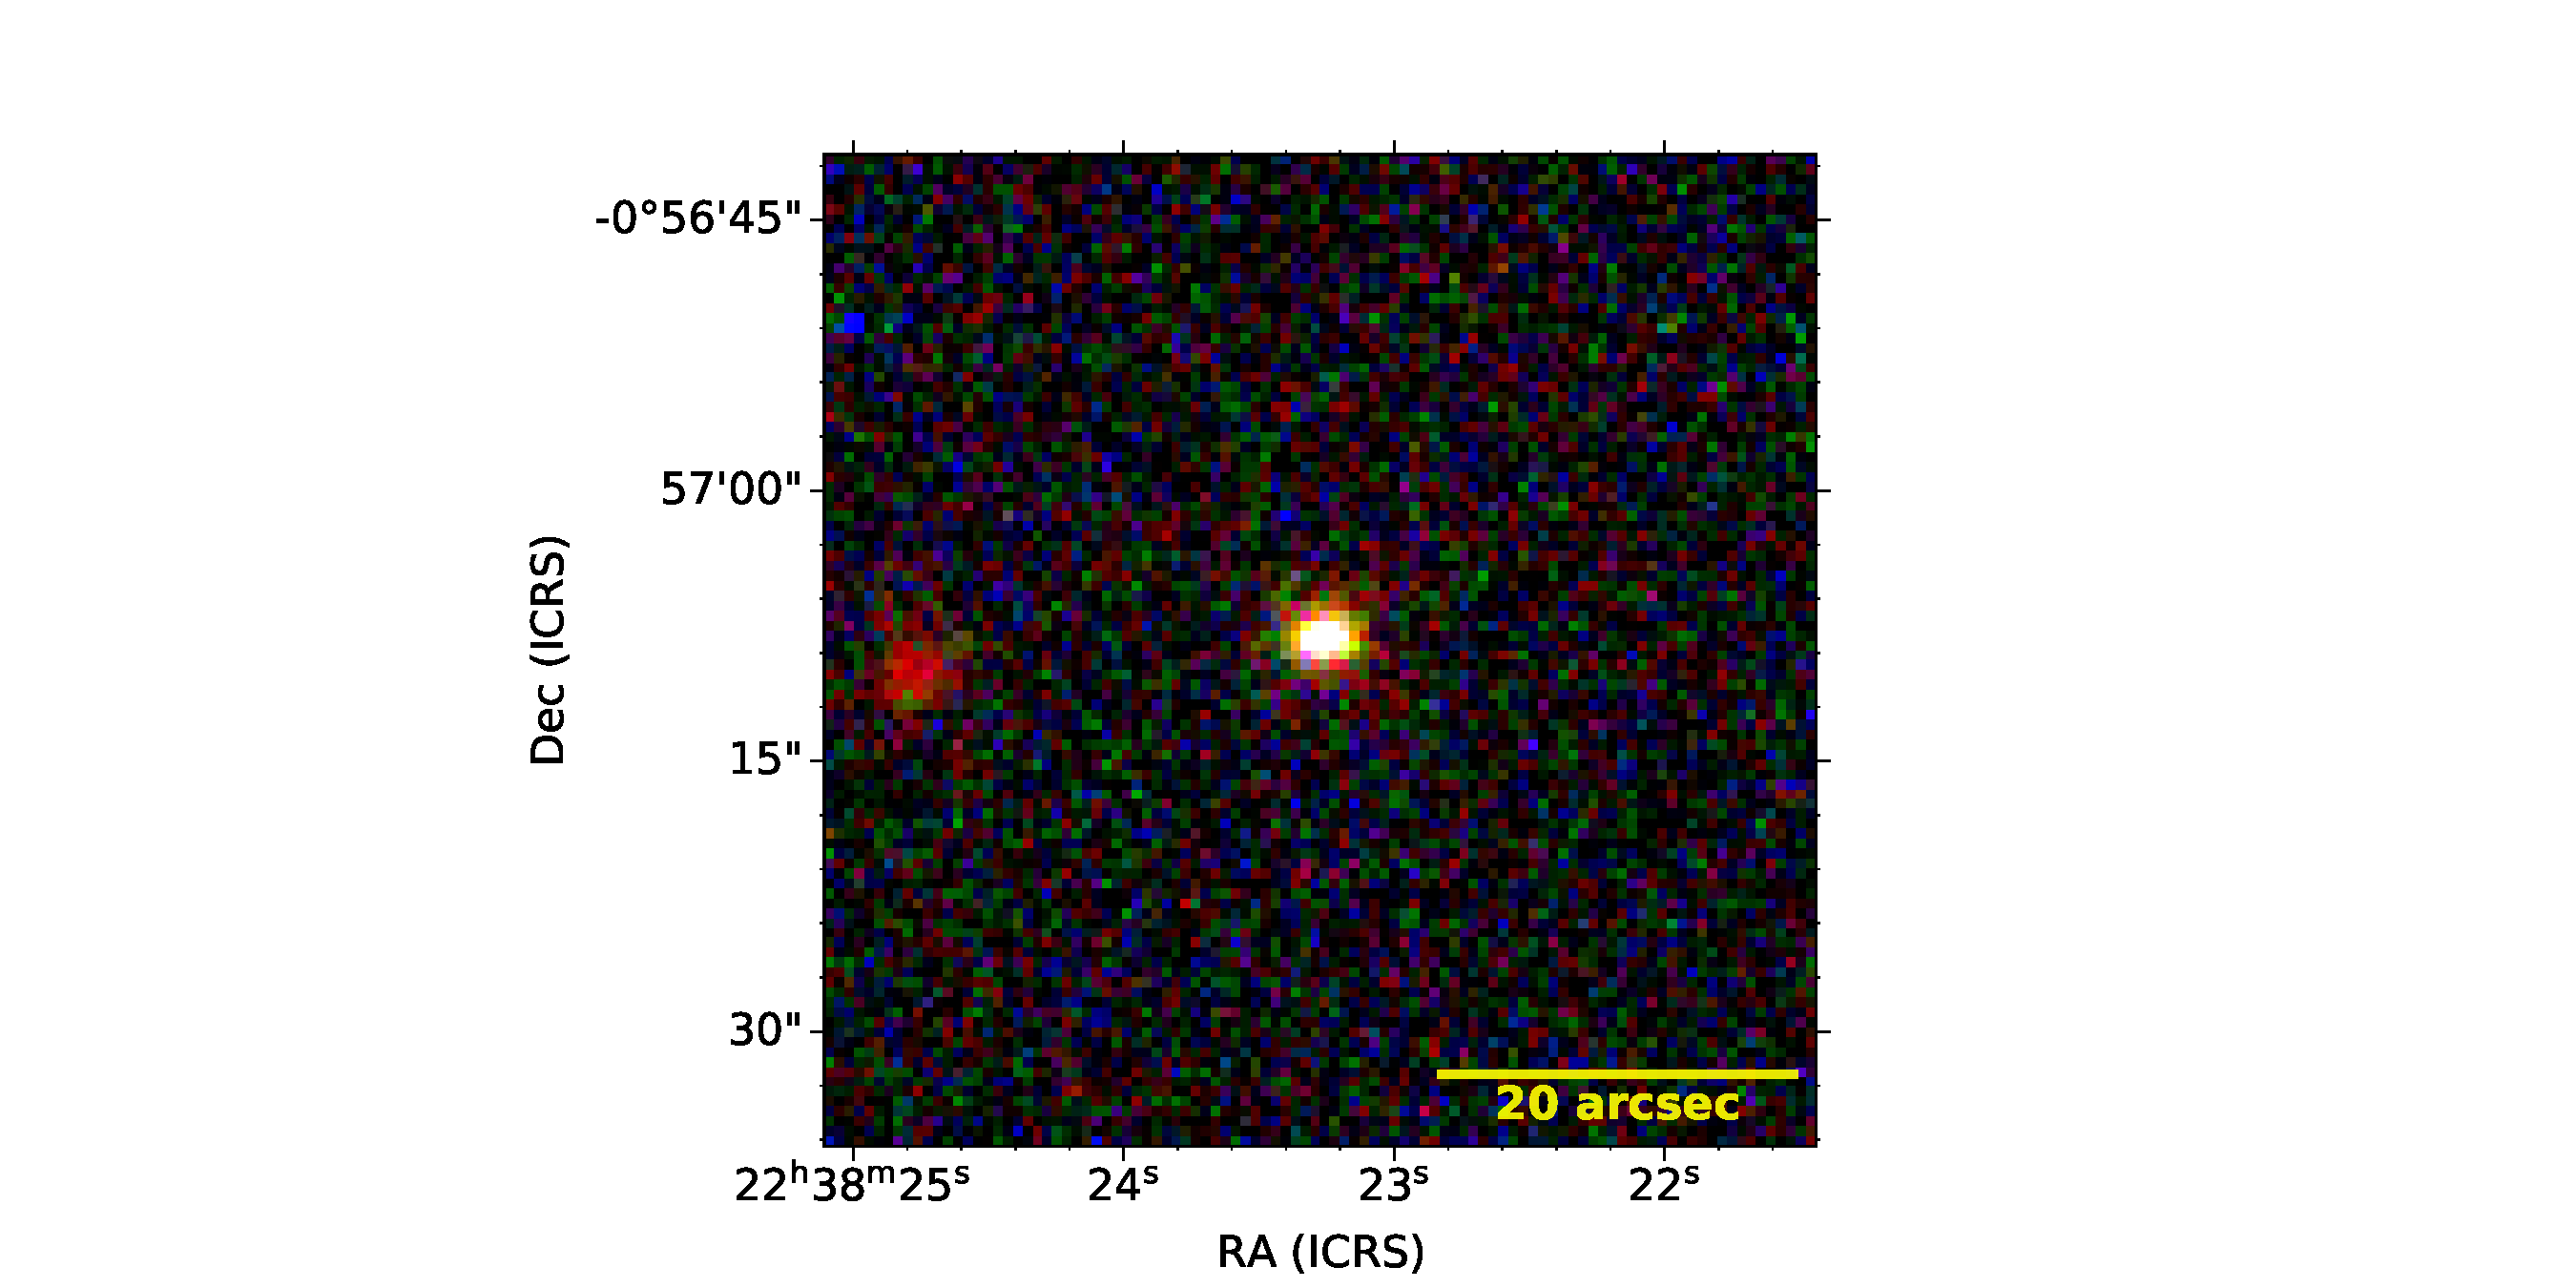
\includegraphics[width=0.4\linewidth, trim=10 0 10 20, clip]{Figs/PHL354_339-0_100_r.pdf} \\
  \end{tabular}
  \caption{Spectra of the known objects select with our algorithm }
  \label{fig:knonw-objects}
\end{figure*}

%% \begin{figure*}
%%   \setlength\tabcolsep{0pt}
%%   \setkeys{Gin}{width=0.5\linewidth}
%%   \begin{tabular}{ll}
%%     (a) & (b) \\
%%     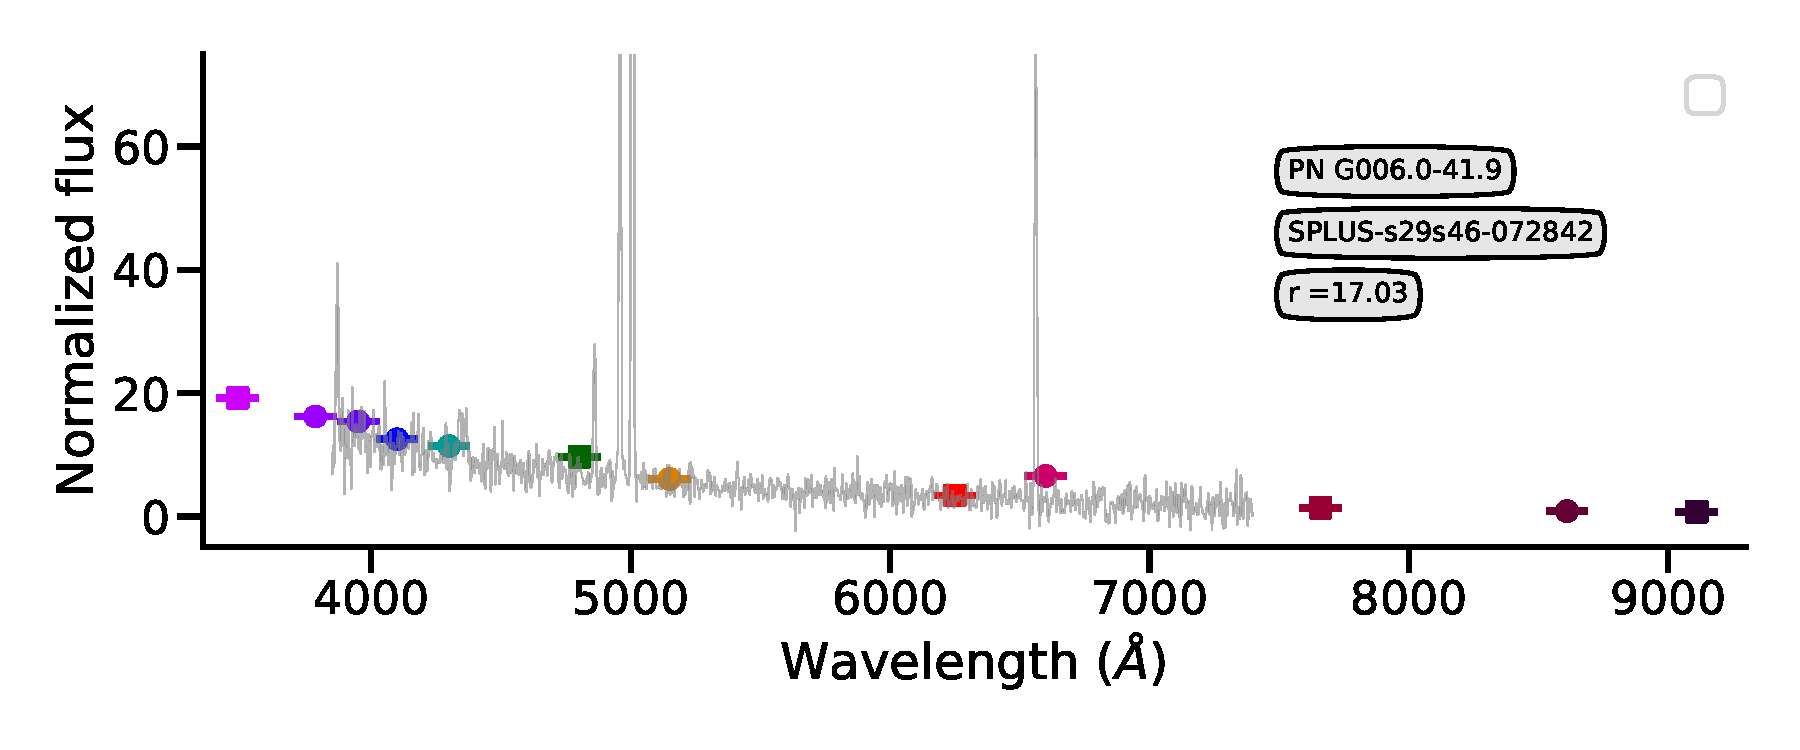
\includegraphics[trim=10 0 5 10, clip]{Figs/StenholmAcker_pn_g006_0-41_9_id176-SPLUS-s29s46-072842.pdf}
%%     & 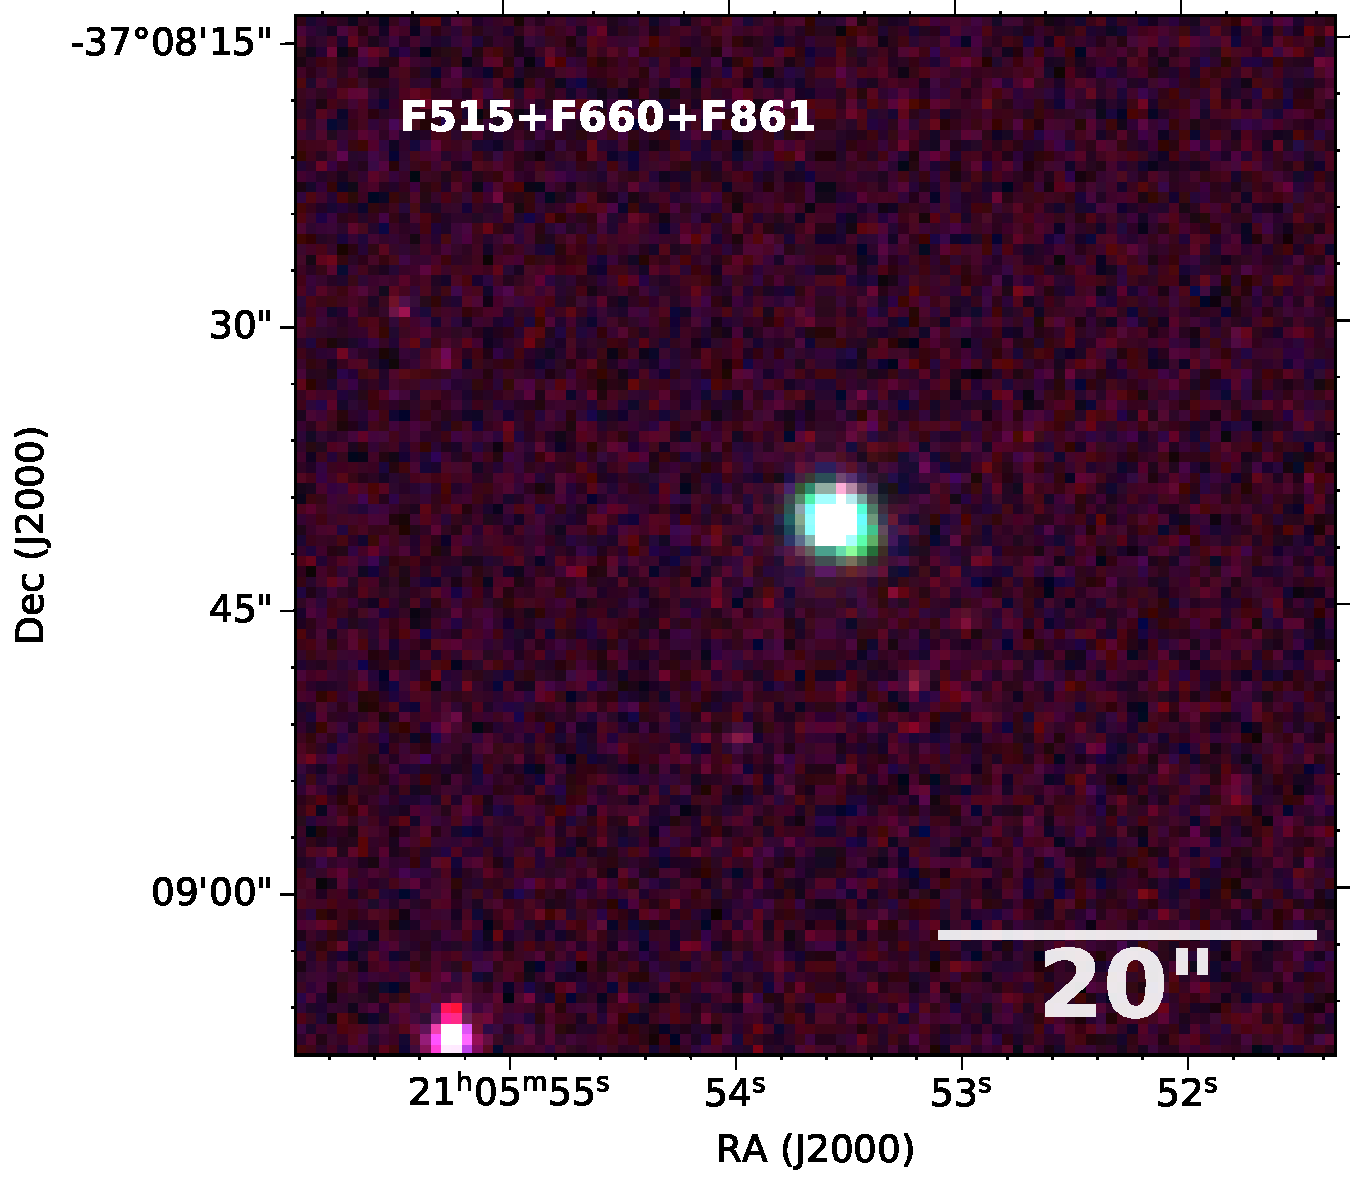
\includegraphics[width=0.2\linewidth, trim=10 0 5 5, clip]{Figs/PNG006_316--37_100_F660-RGB.pdf} \\
%%     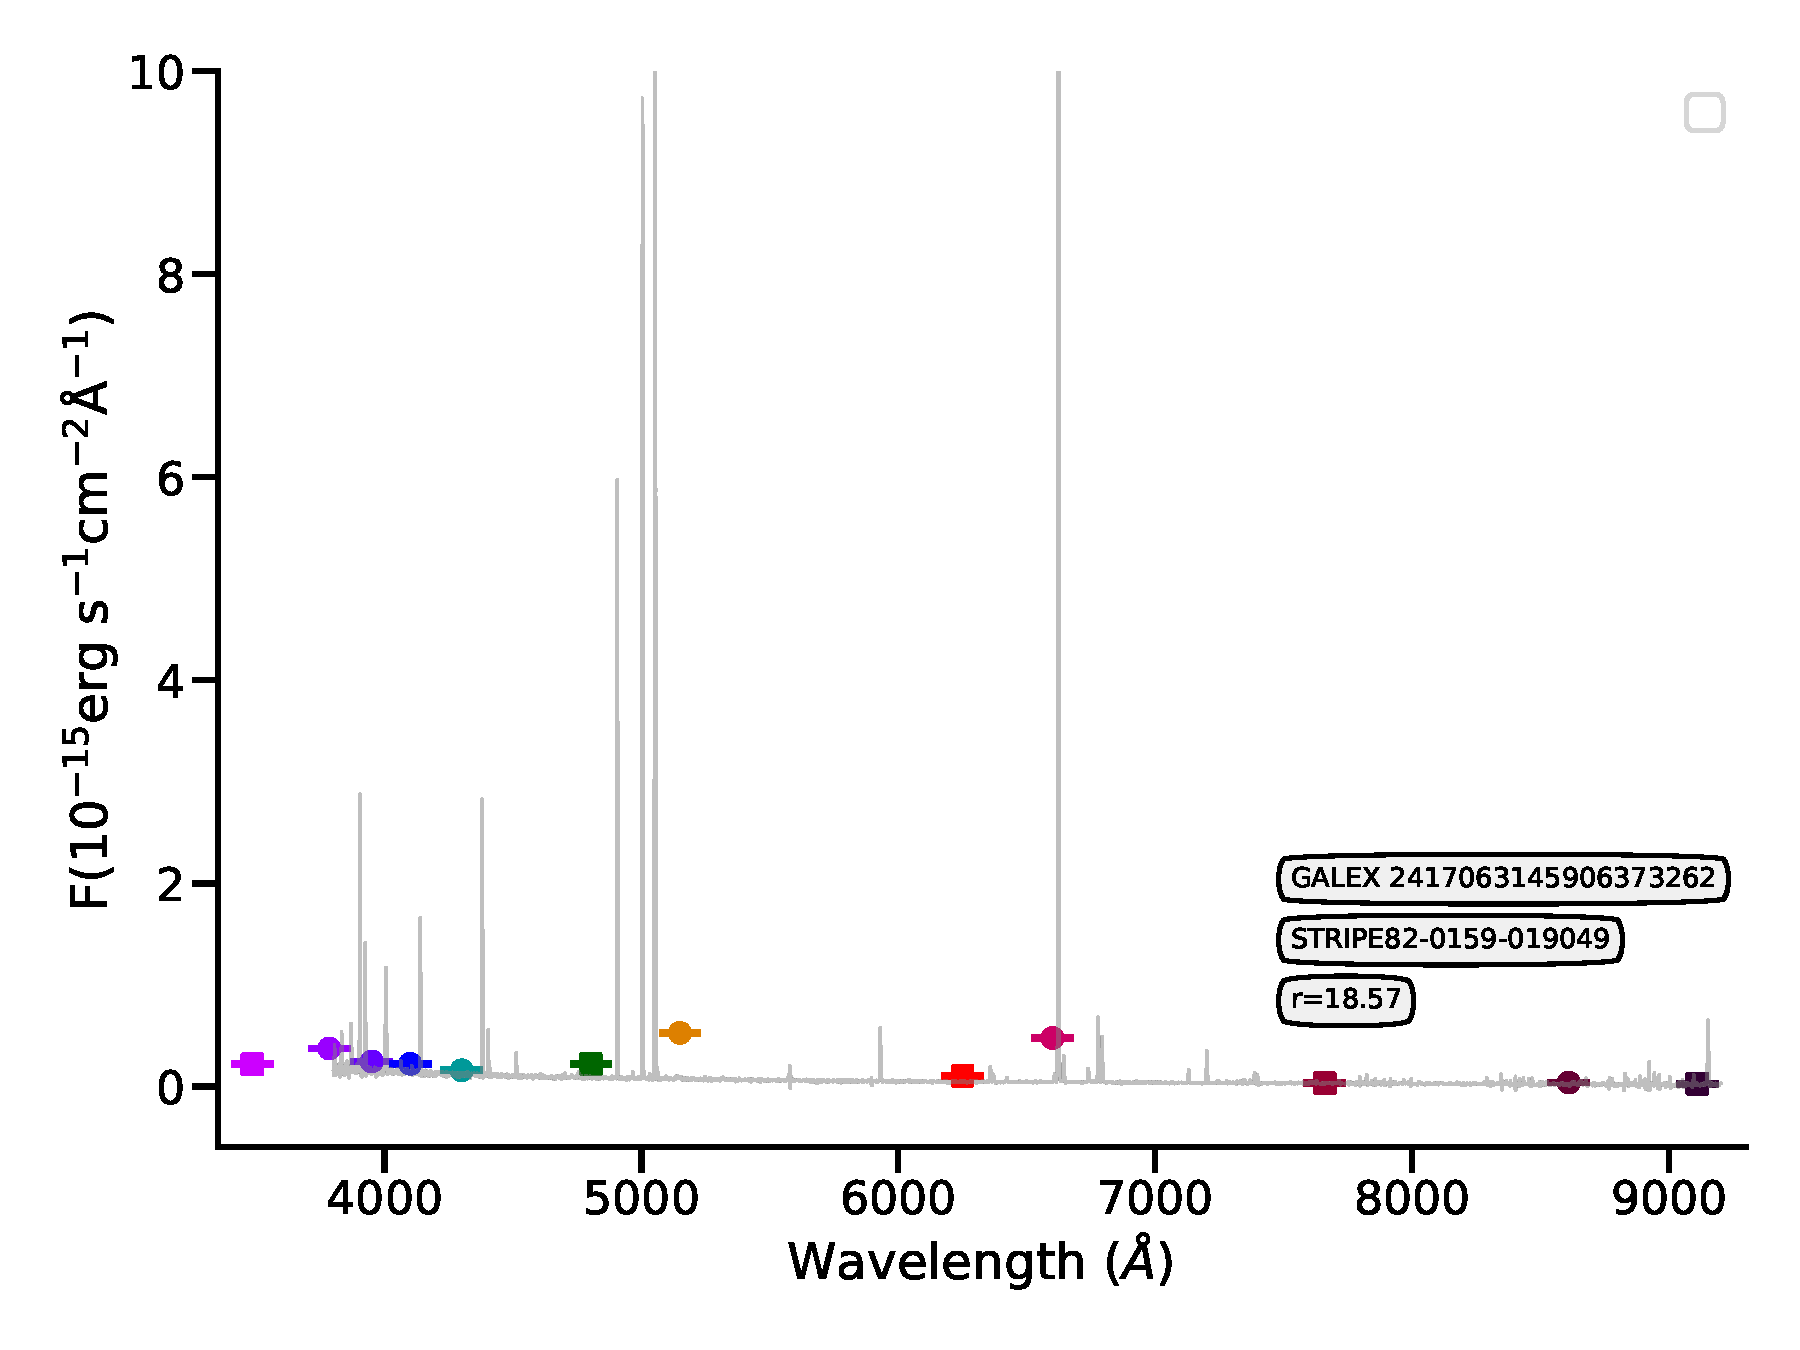
\includegraphics[trim=10 0 5 10, clip]{Figs/spec-0680-52200-0153-STRIPE82-0159-019049.pdf}
%%     & 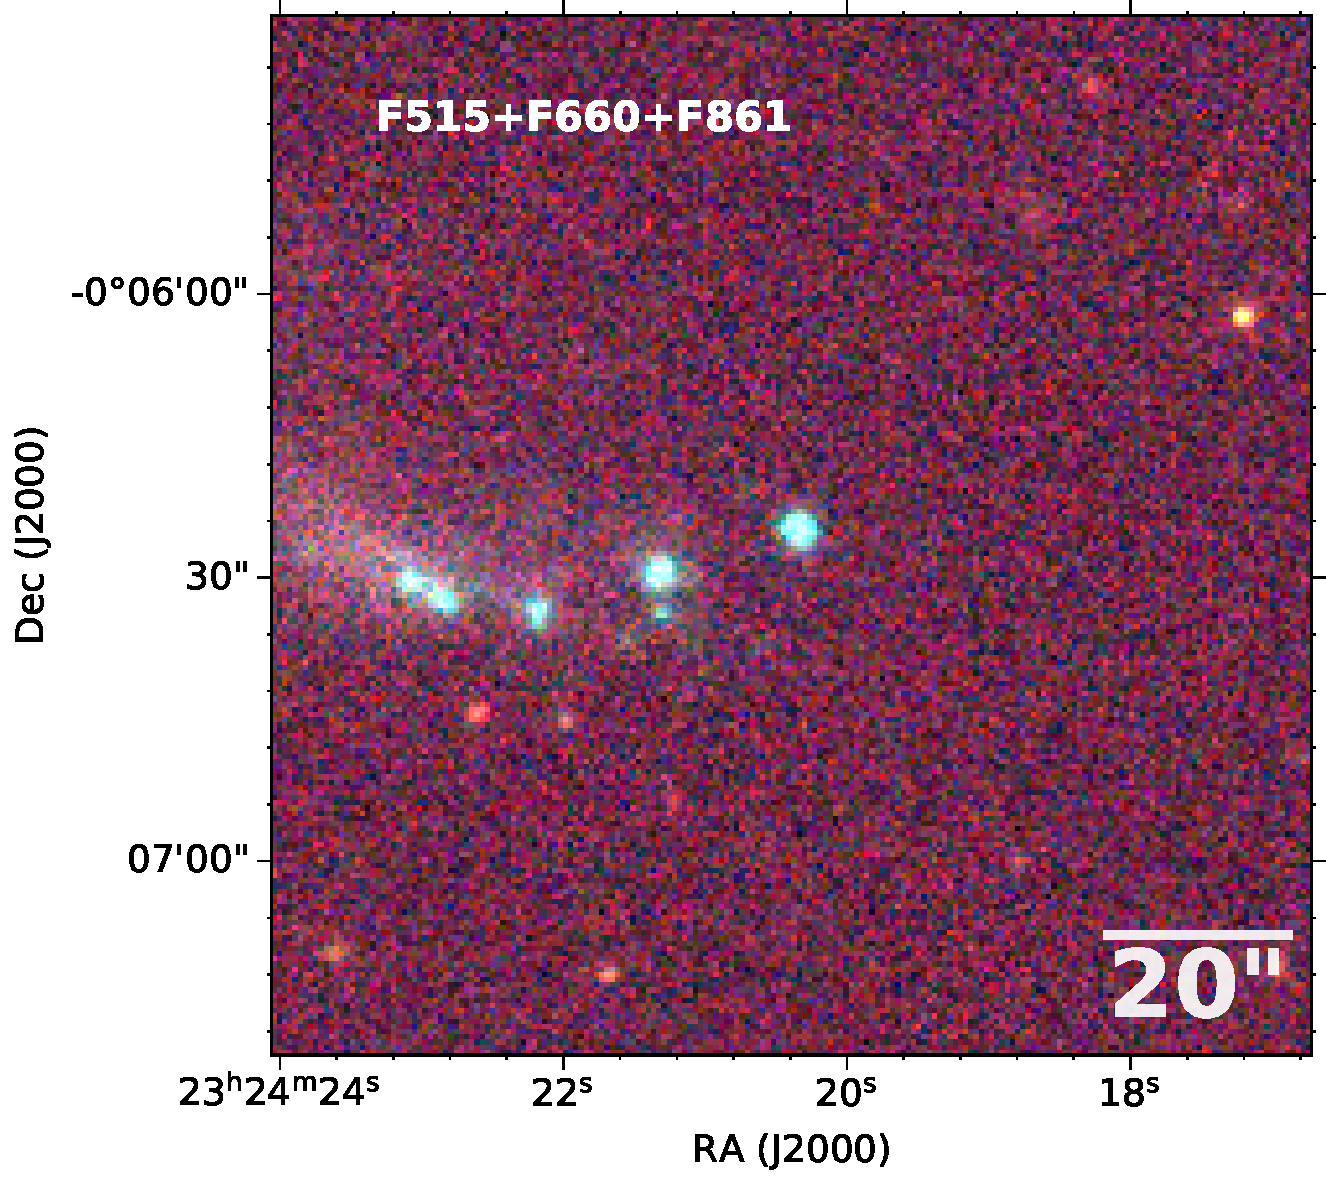
\includegraphics[width=0.2\linewidth, trim=10 0 5 5, clip]{Figs/GALEX24170_351-0_200_F660-RGB.pdf} \\
%%     (c) & (d) \\
%%     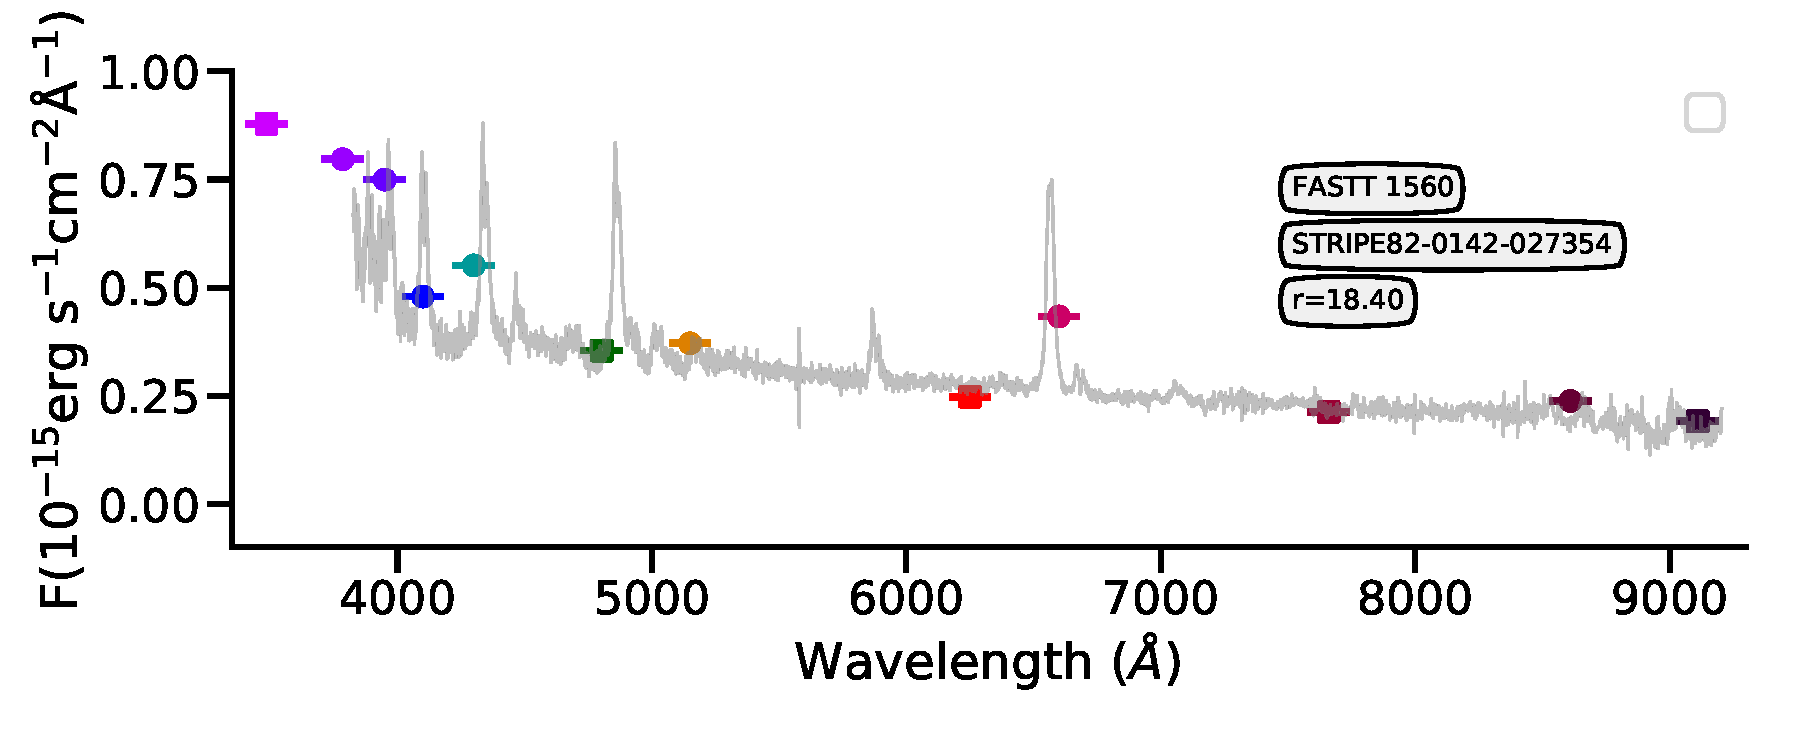
\includegraphics[trim=10 0 5 10, clip]{Figs/spec-0376-52143-0631-STRIPE82-0142-027354.pdf}
%%     & 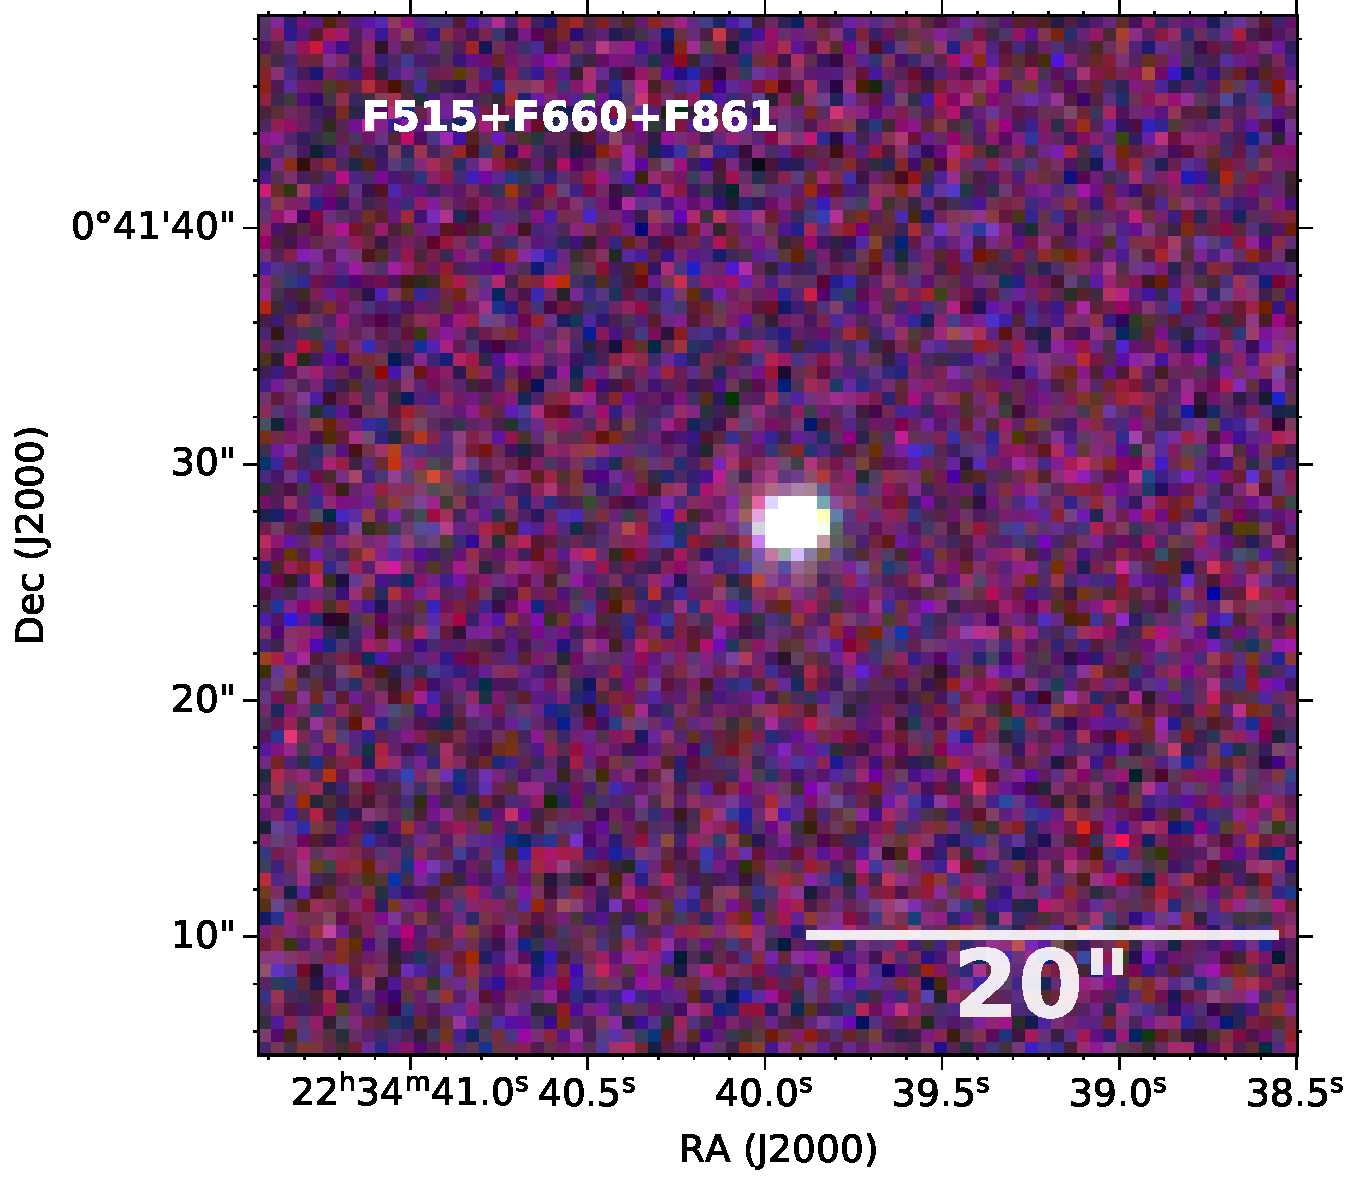
\includegraphics[width=0.2\linewidth, trim=10 0 5 5, clip]{Figs/FASTT1560_338-0_80_F660-RGB.pdf} \\
%%     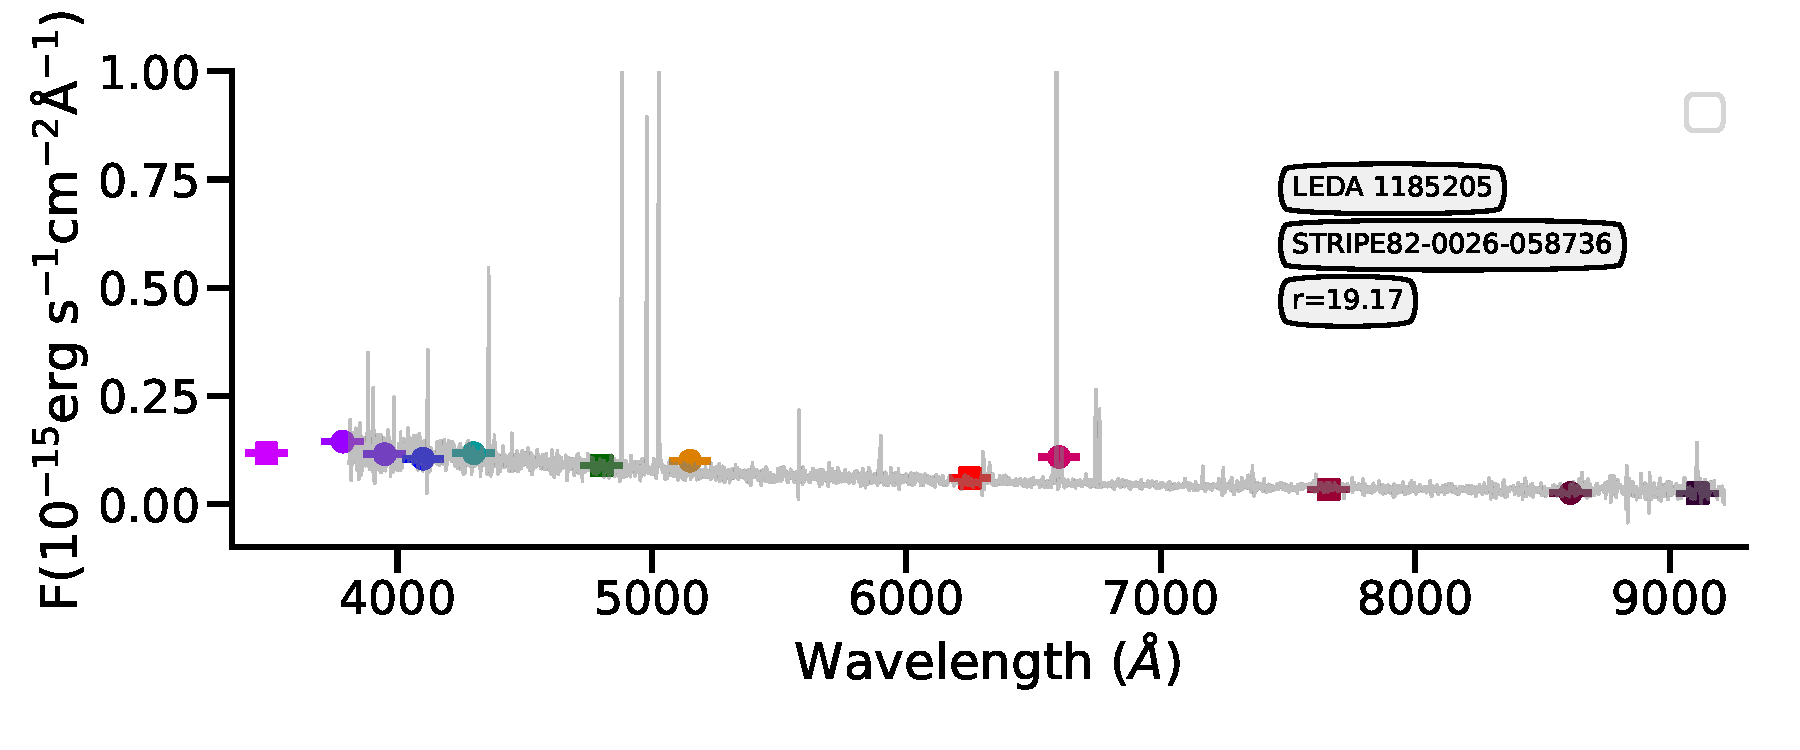
\includegraphics[trim=10 0 5 10, clip]{Figs/spec-0397-51794-0336-STRIPE82-0026-058736.pdf}
%%     & 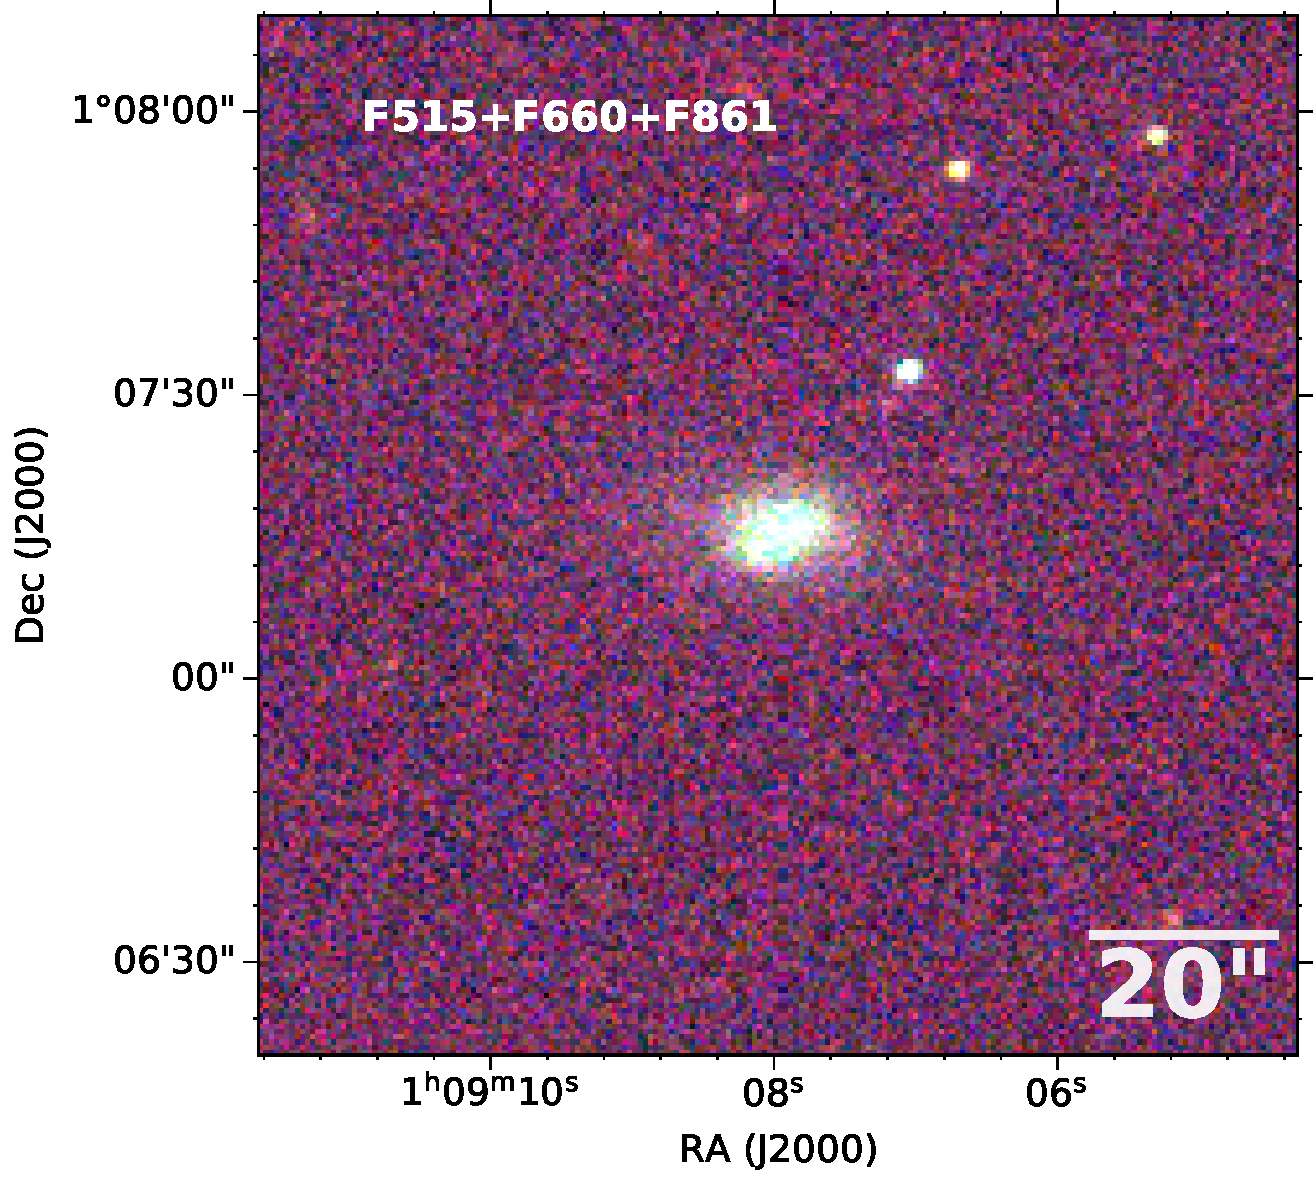
\includegraphics[width=0.2\linewidth, trim=10 0 5 5, clip]{Figs/LEDA1185205_17-1_200_F660-RGB.pdf} \\
%%     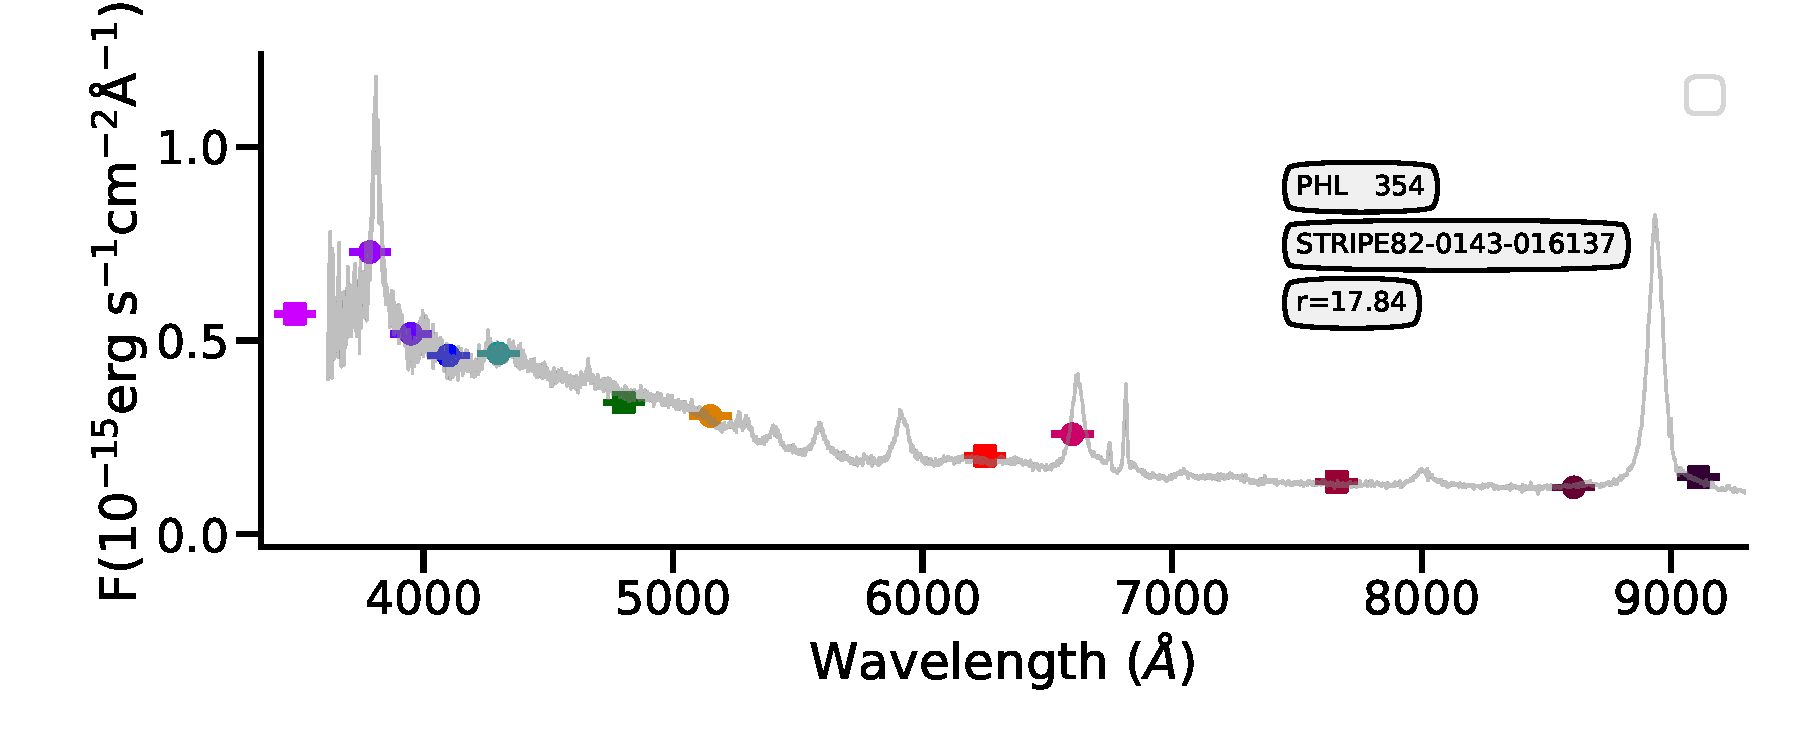
\includegraphics[trim=10 0 5 10, clip]{Figs/spec-9217-57934-0839-STRIPE82-0143-016137.pdf}
%%     & 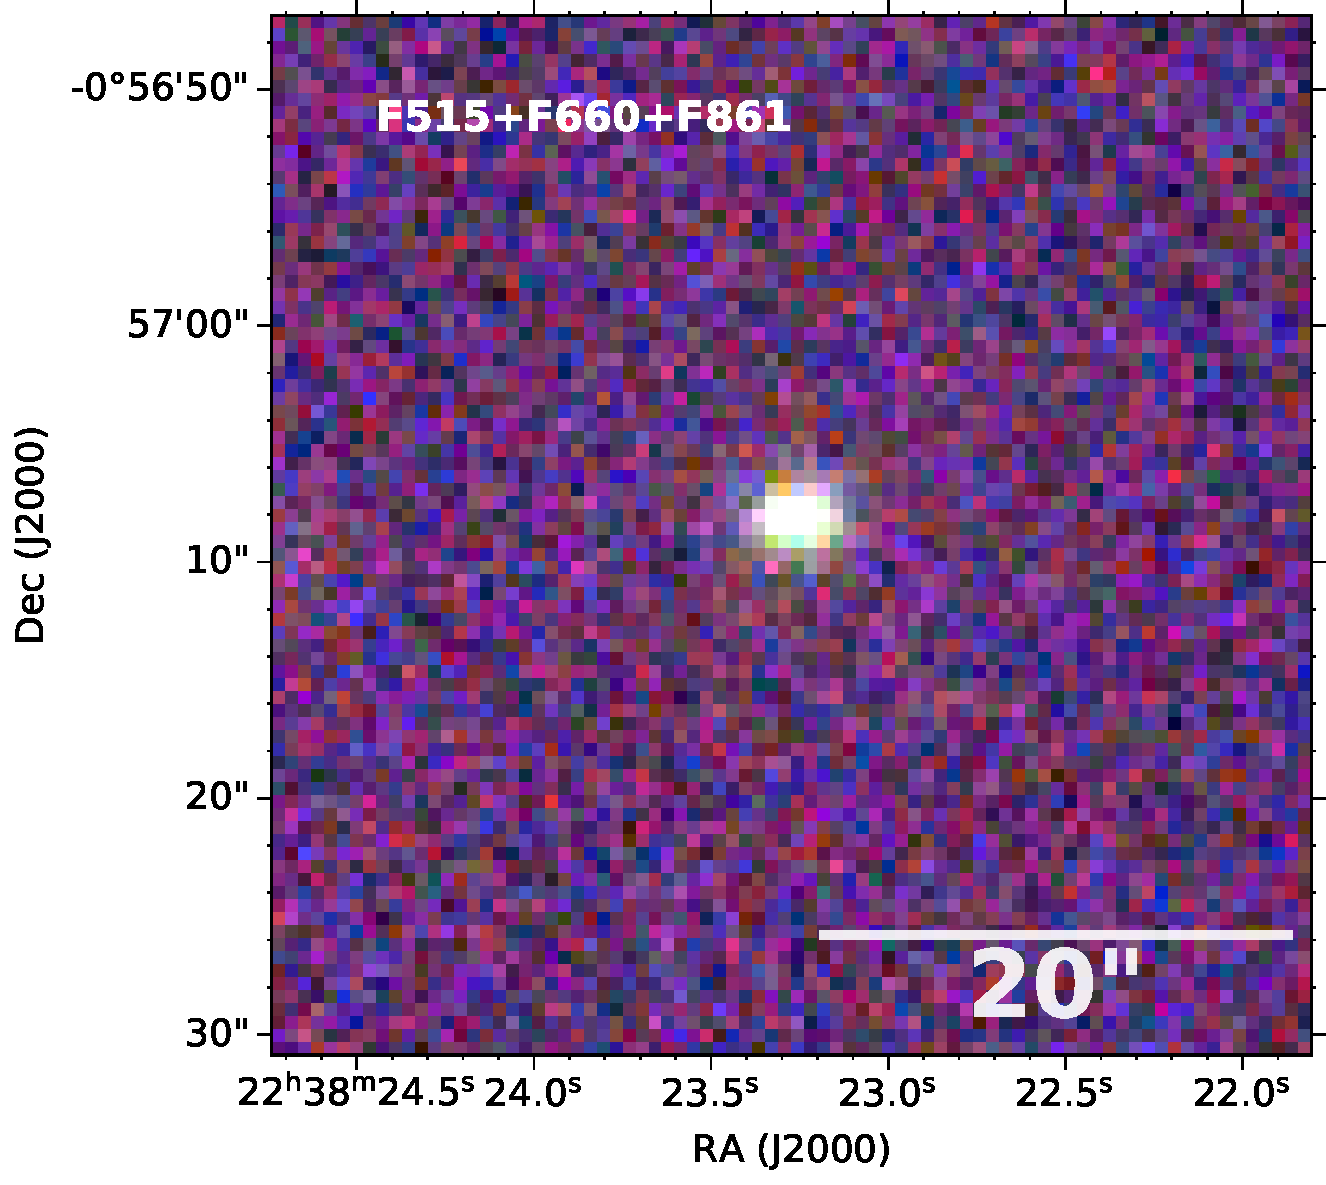
\includegraphics[width=0.2\linewidth, trim=10 0 5 5, clip]{Figs/PHL354_339-0_80_F660-RGB.pdf} \\
%%   \end{tabular}
%%   \caption{Spectra of the known objects select with our algorithm }
%%   \label{fig:knonw-objects}
%% \end{figure*}

\begin{figure*}
  \setlength\tabcolsep{0pt}
  \setkeys{Gin}{width=0.5\linewidth}
  \begin{tabular}{ll}
    (a) & (b) \\
    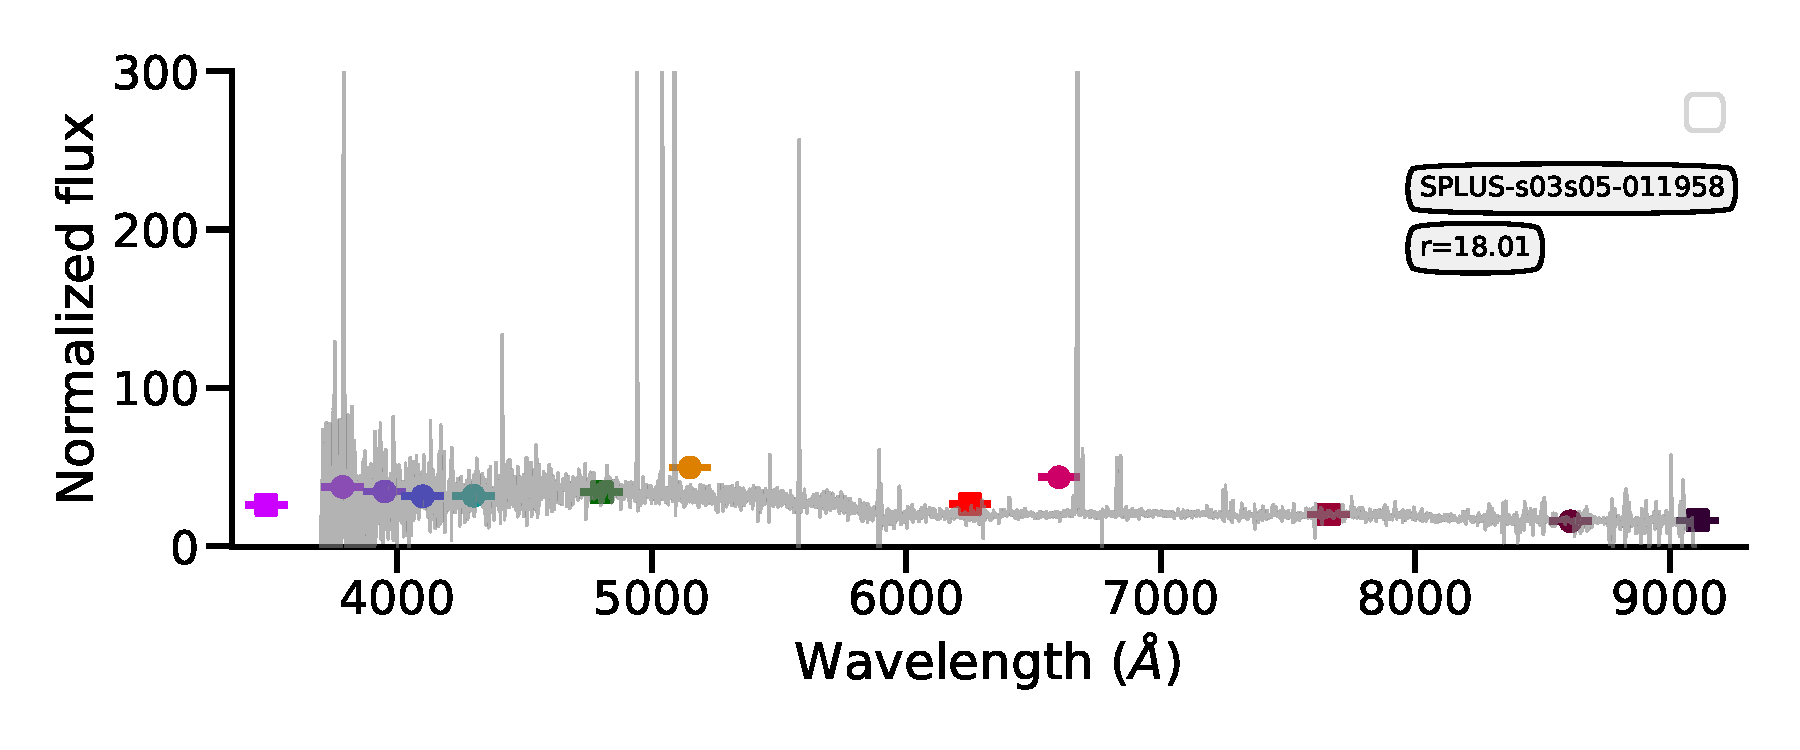
\includegraphics[trim=10 0 10 20, clip]{Figs/spec-57313-EG220318S020919M01_sp10-173-SPLUS-s03s05-011958.pdf}
    & 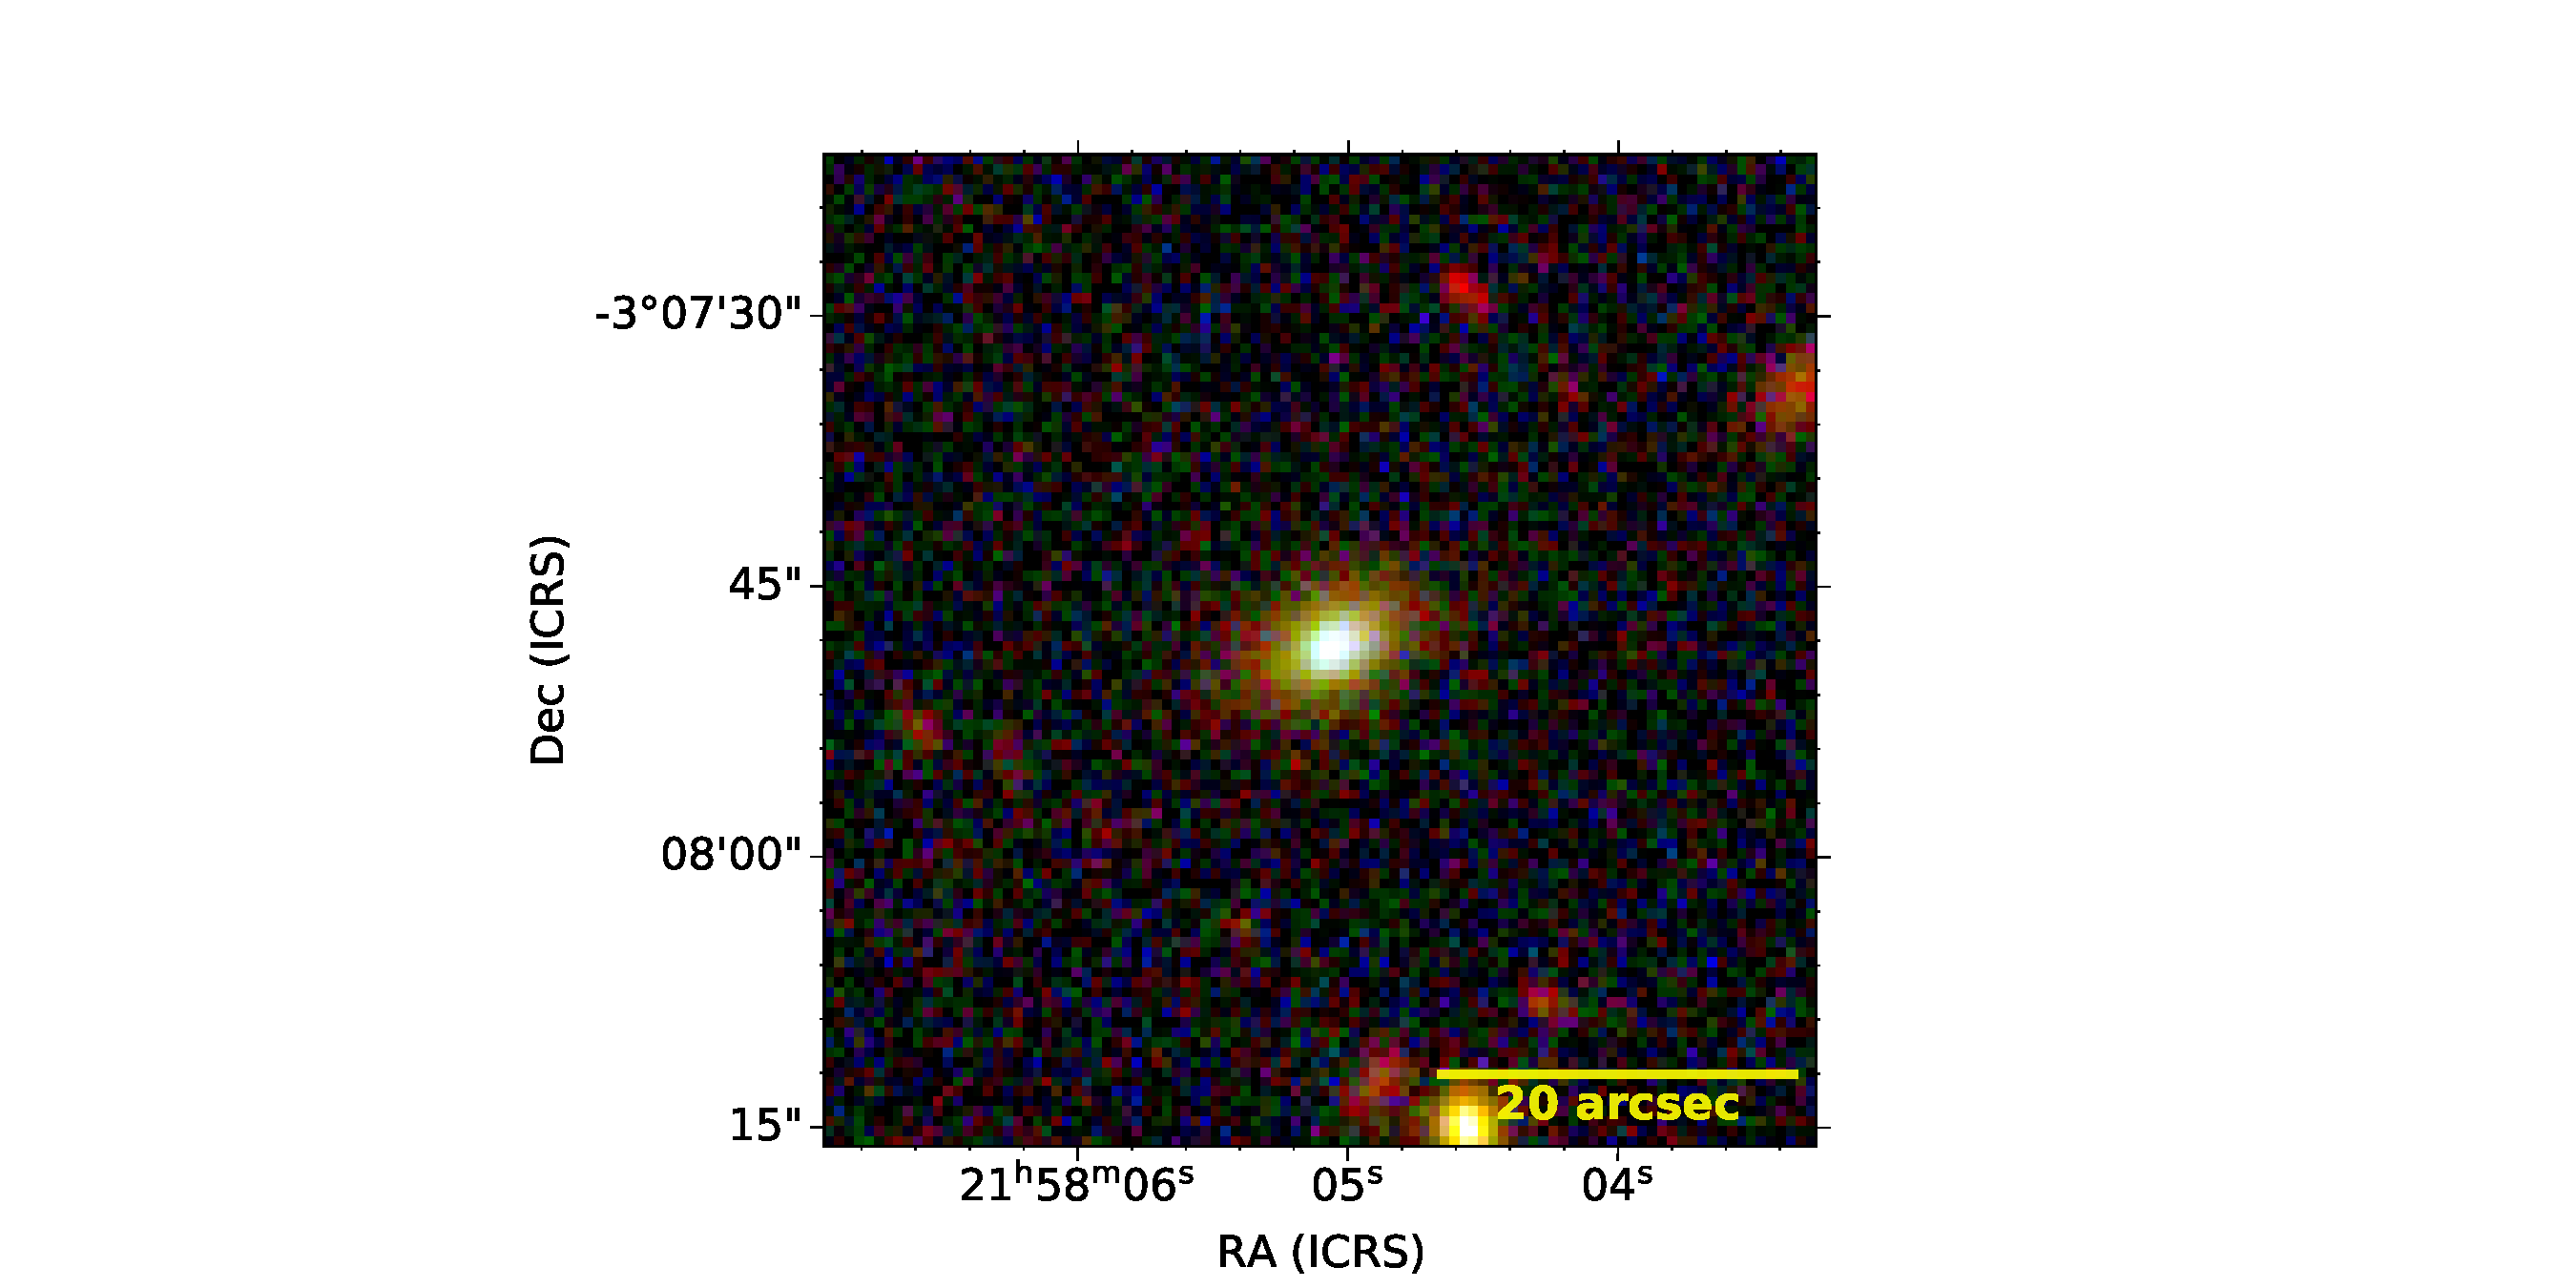
\includegraphics[width=0.4\linewidth, trim=10 0 10 20, clip]{Figs/SPLUS-s03s05-011958_329-3_100_r.pdf} \\
    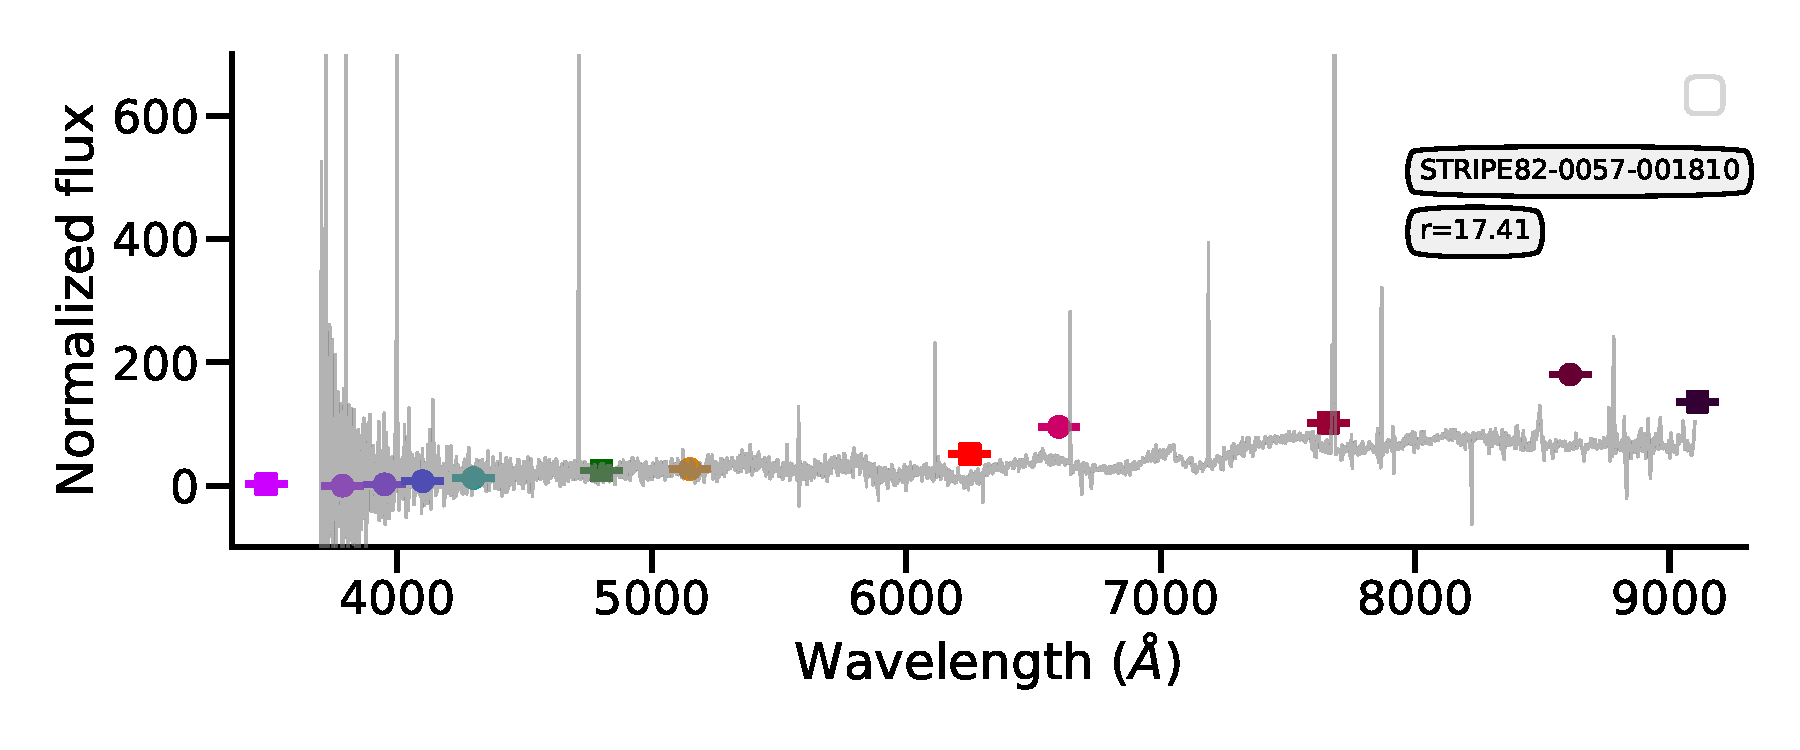
\includegraphics[trim=10 0 10 20, clip]{Figs/spec-55893-F9304_sp15-198-STRIPE82-0057-001810.pdf}
    & 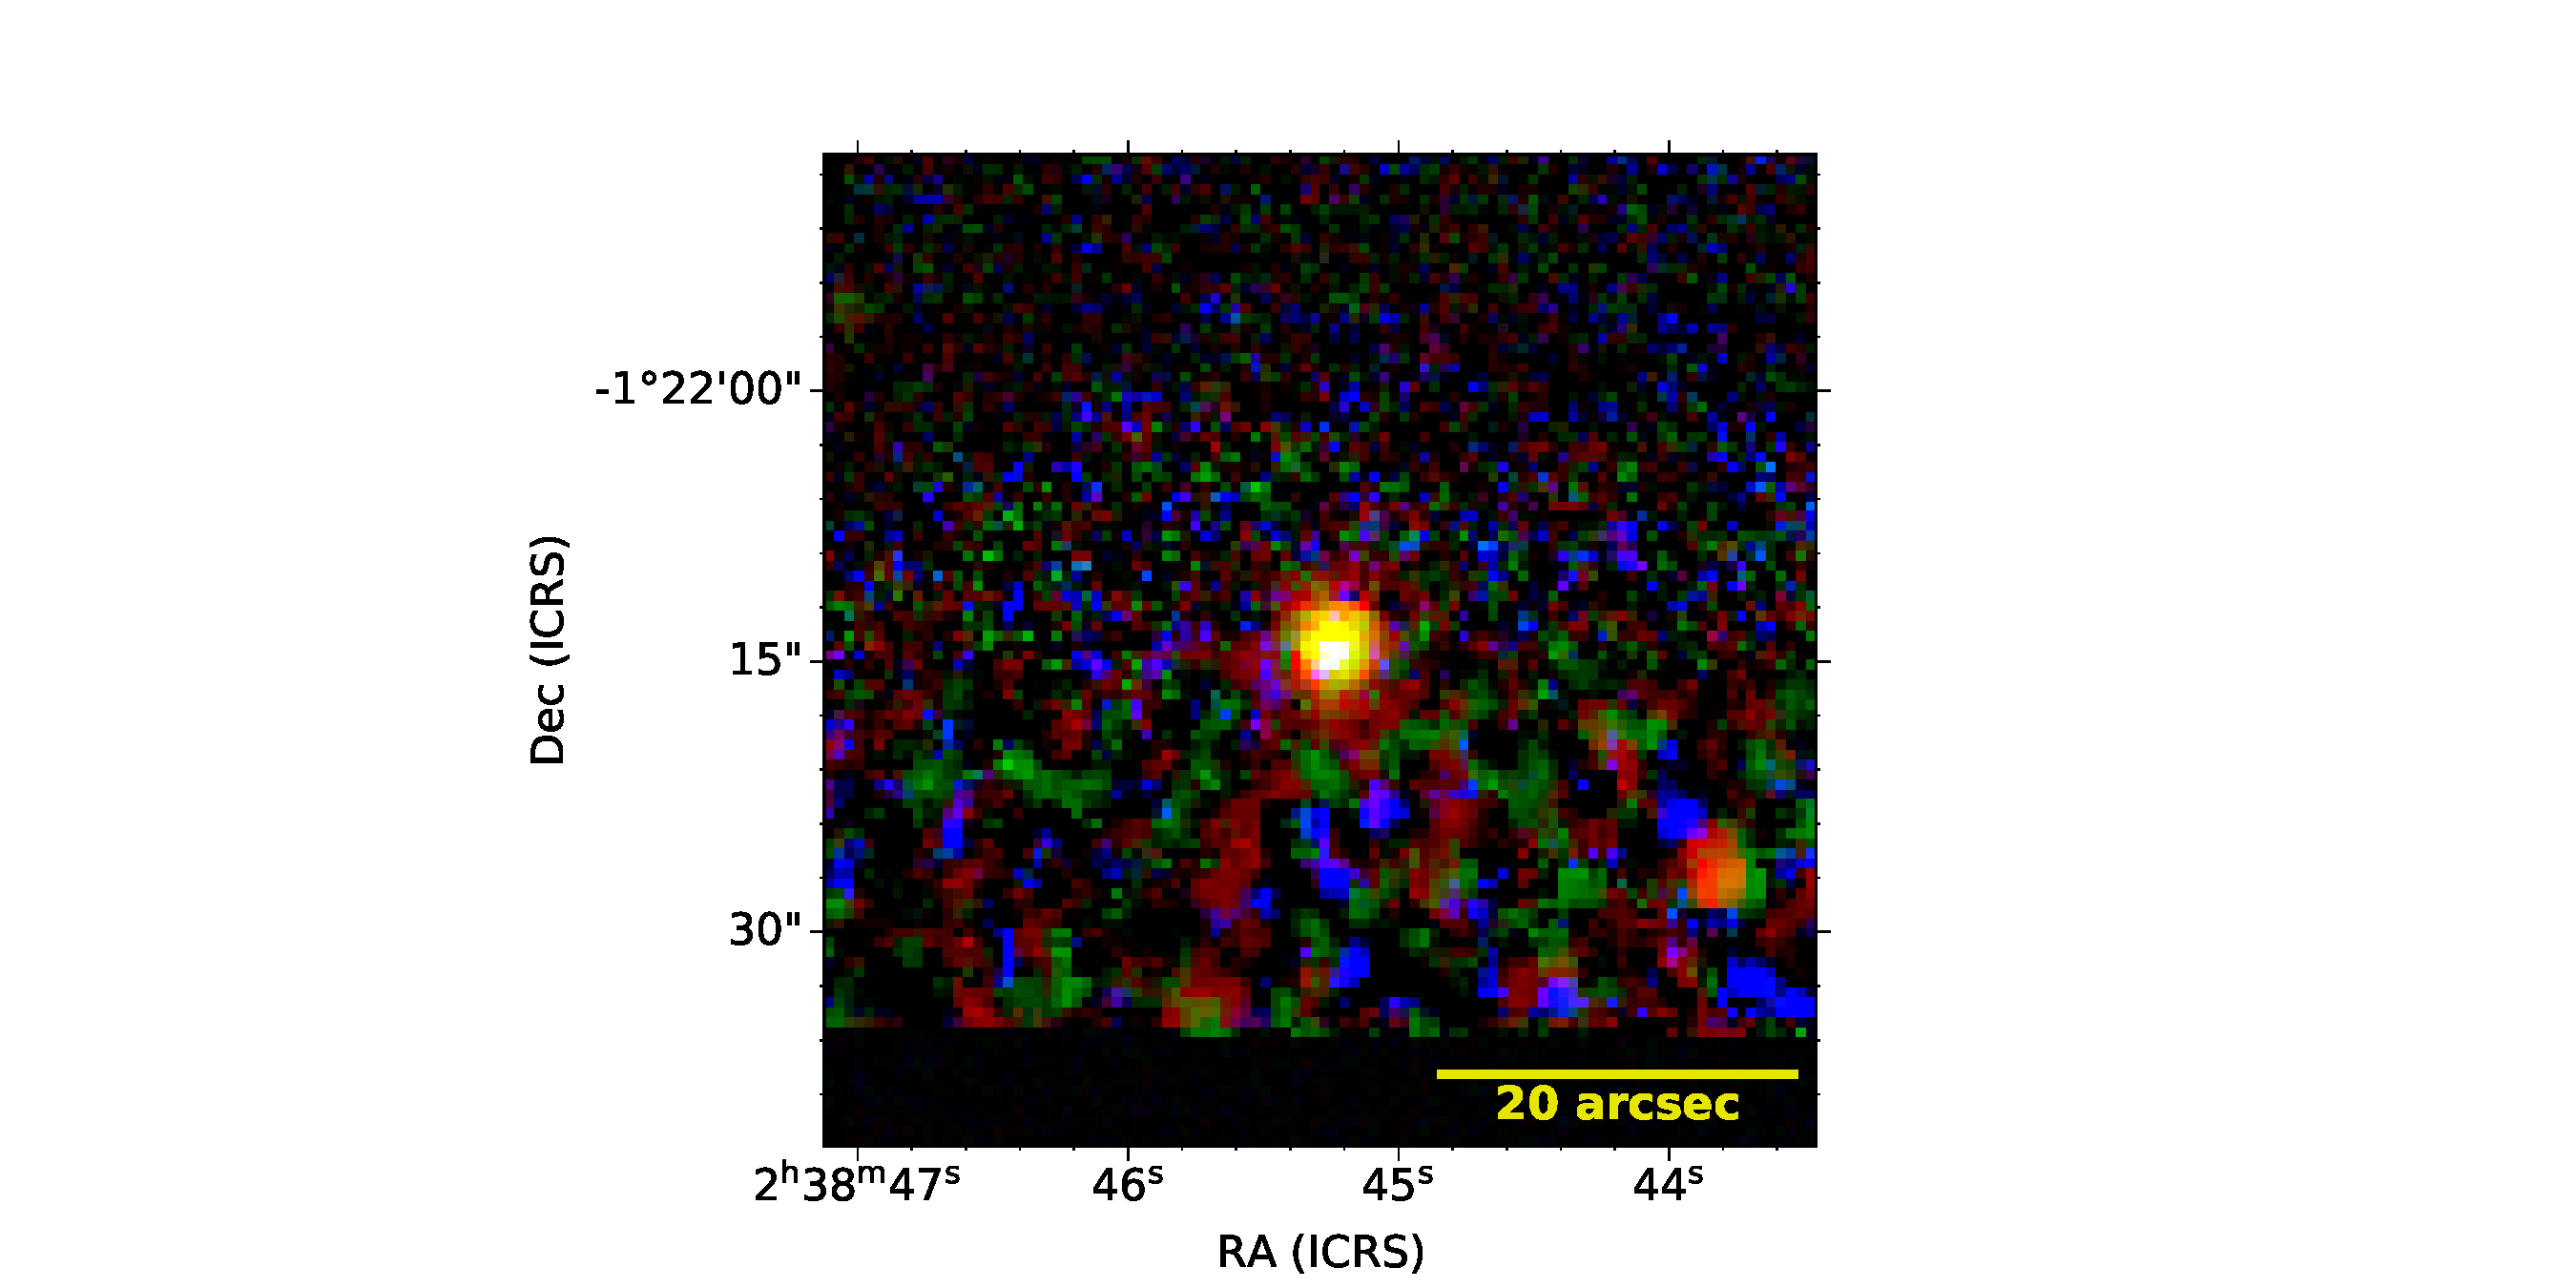
\includegraphics[width=0.4\linewidth, trim=10 0 10 20, clip]{Figs/STRIPE82-0057-001810_39-1_100_r.pdf} \\
    (c) & (d) \\
    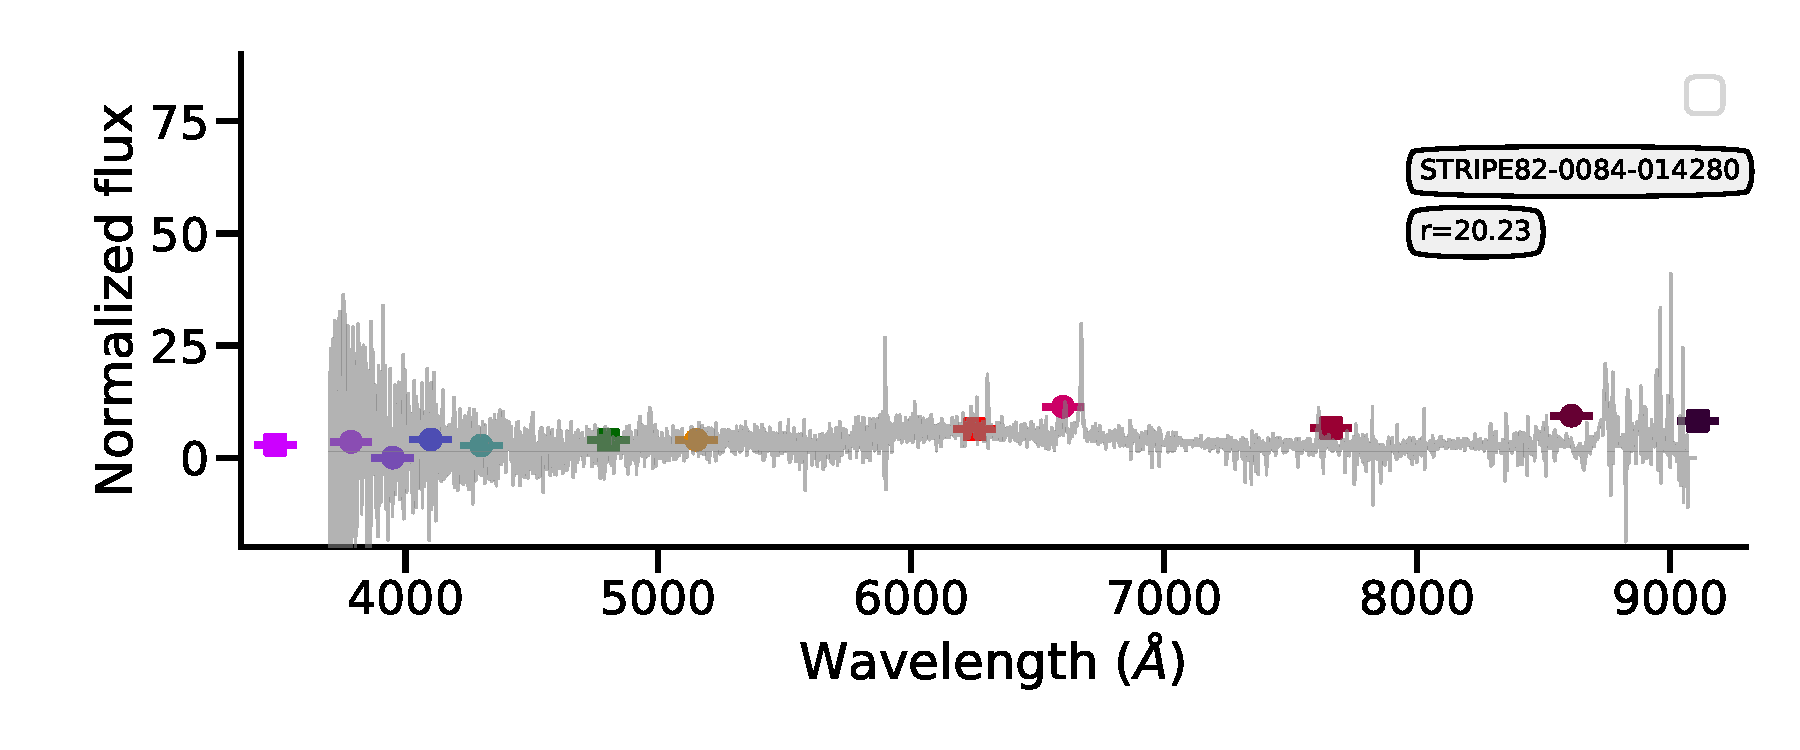
\includegraphics[trim=10 0 10 20, clip]{Figs/spec-57336-EG034838N001340M01_sp09-025-STRIPE82-0084-014280.pdf}
    & 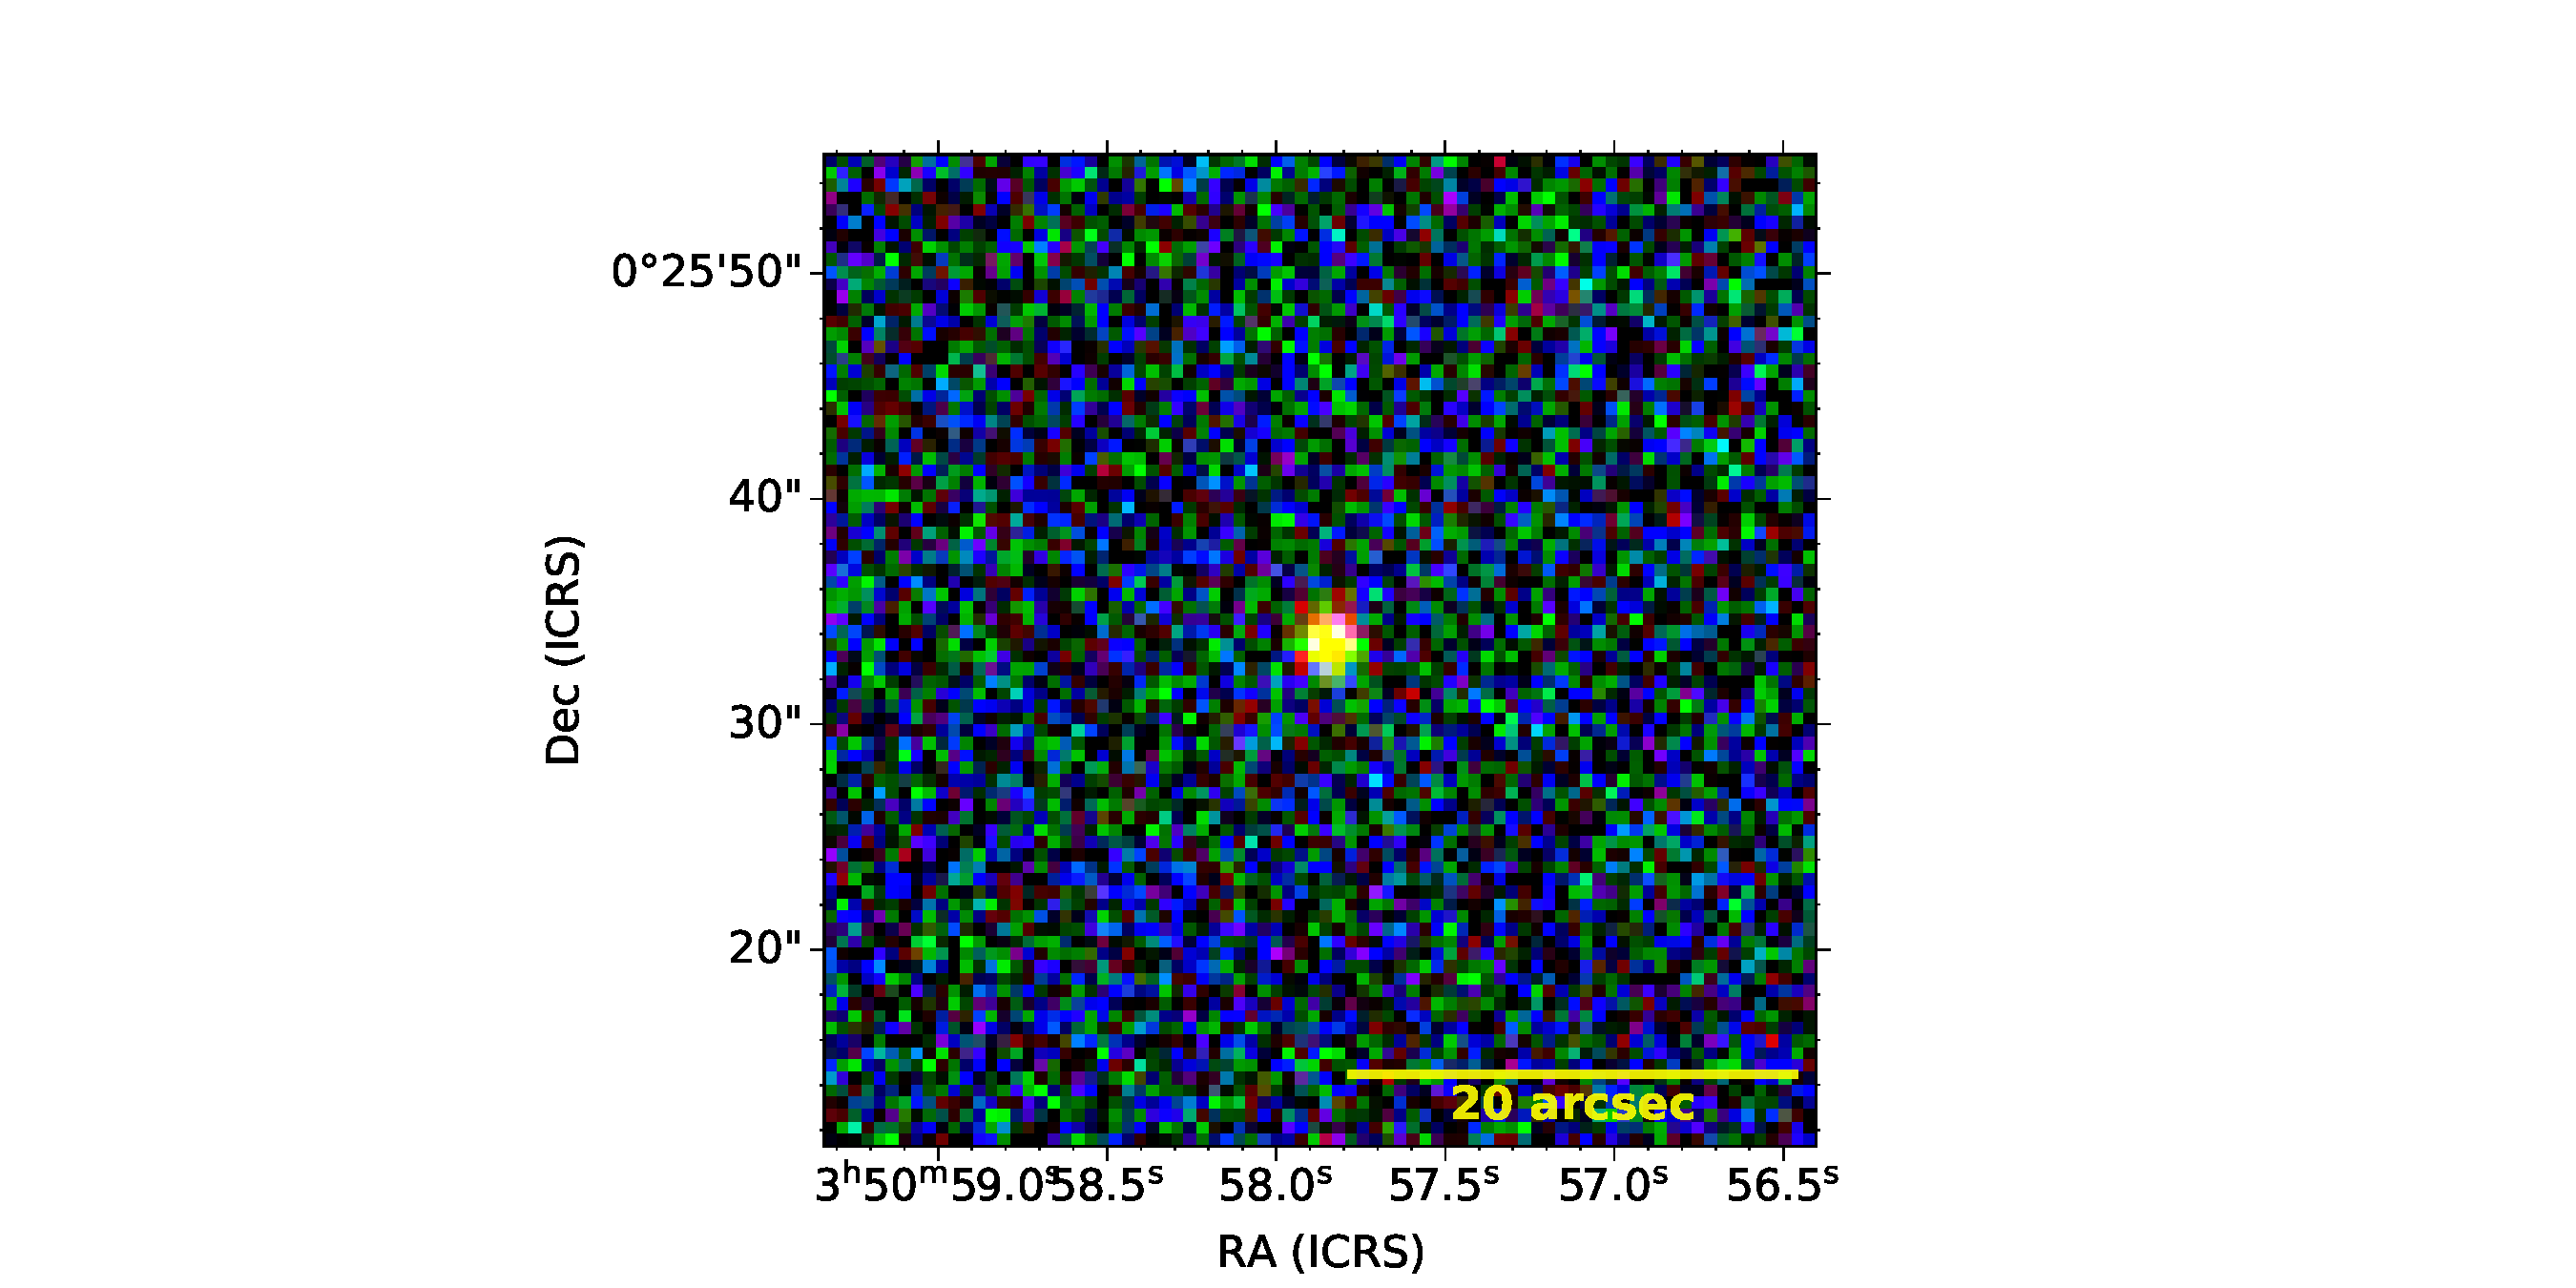
\includegraphics[width=0.4\linewidth, trim=10 0 10 20, clip]{Figs/STRIPE82-0084-014280_57-0_80_r.pdf} \\
  \end{tabular}
  \caption{Spectra of the Lamost }
  \label{fig:color-diagram}
\end{figure*}

\begin{figure*}
  \setlength\tabcolsep{0pt}
  \setkeys{Gin}{width=0.5\linewidth}
  \begin{tabular}{ll}
    (a) & (b) \\
    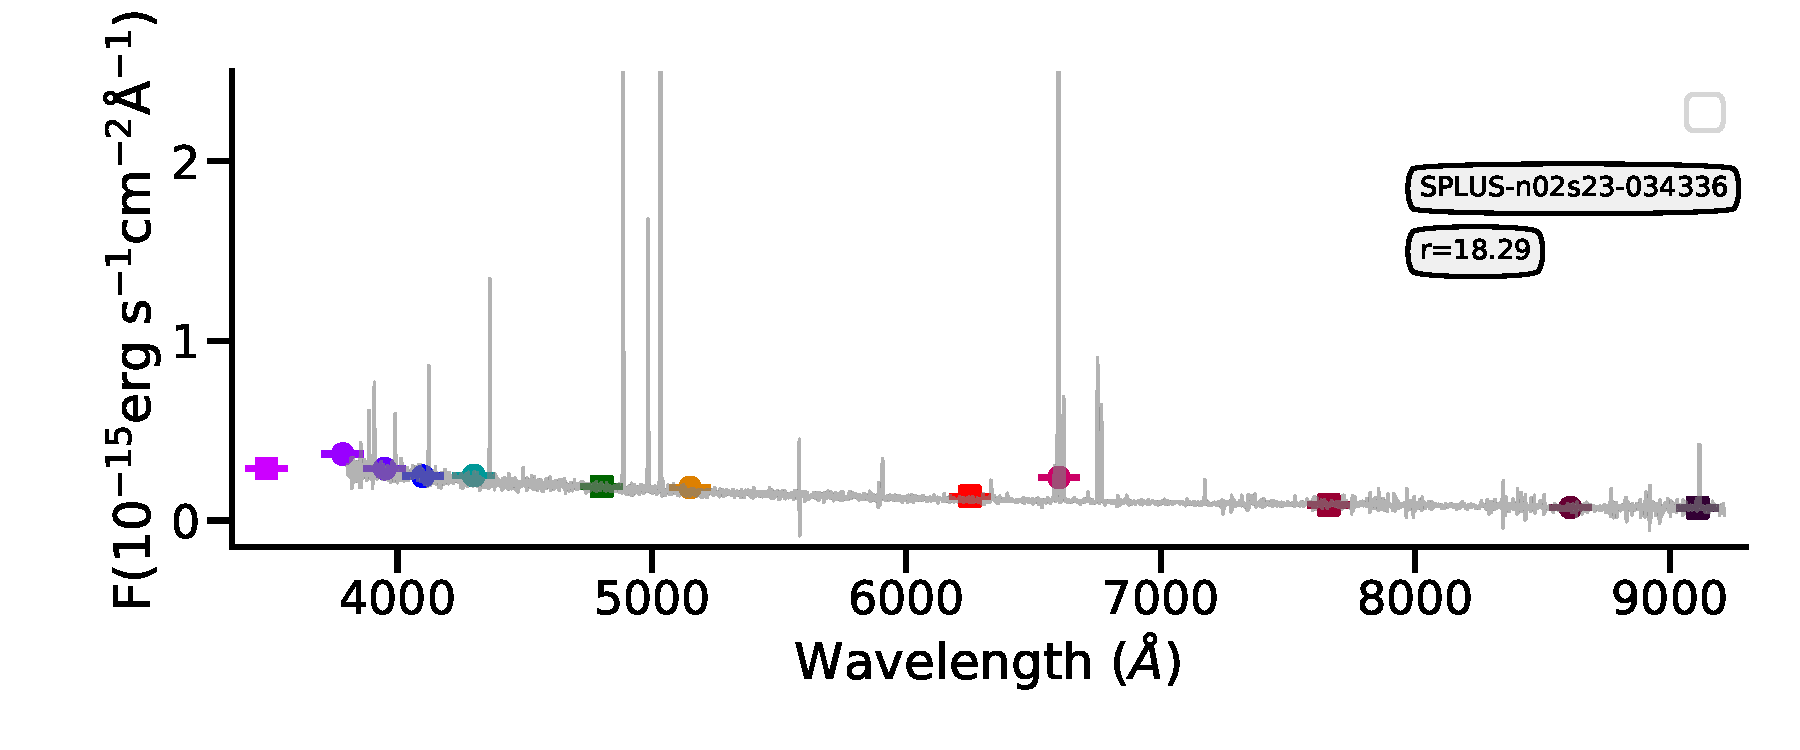
\includegraphics[trim=10 0 10 20, clip]{Figs/spec-0331-52368-0449-SPLUS-n02s23-034336.pdf}
    & 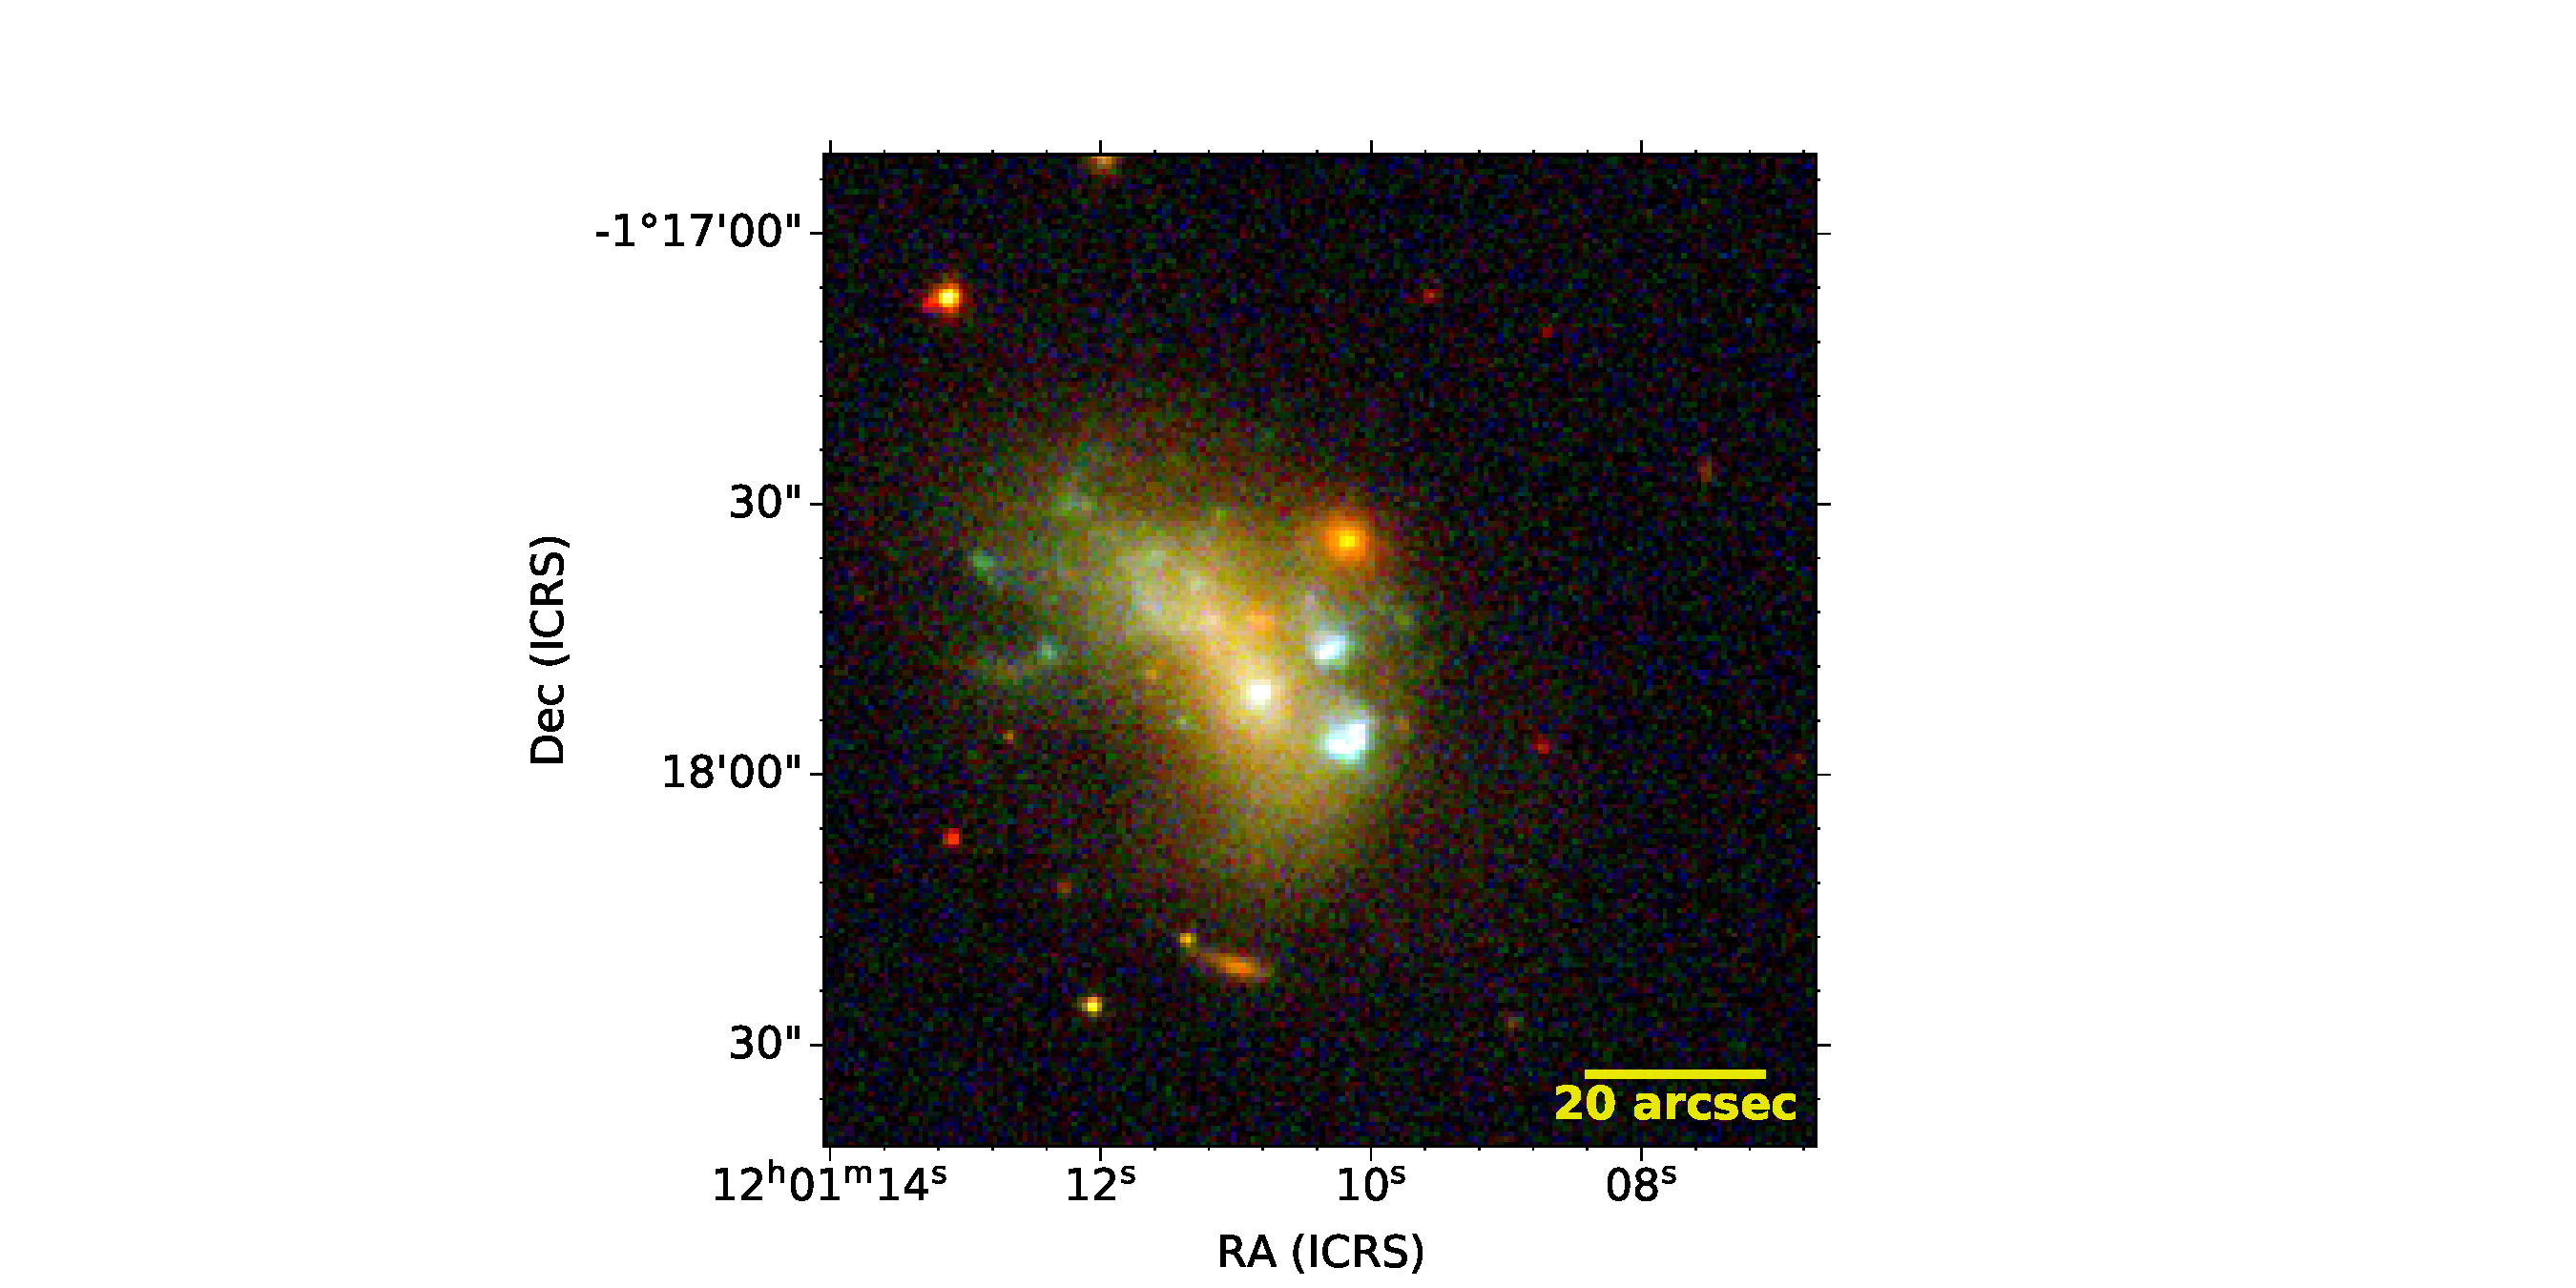
\includegraphics[width=0.4\linewidth, trim=10 0 10 20, clip]{Figs/SPLUS-n02s23-034336_180-1_200_r.pdf} \\
    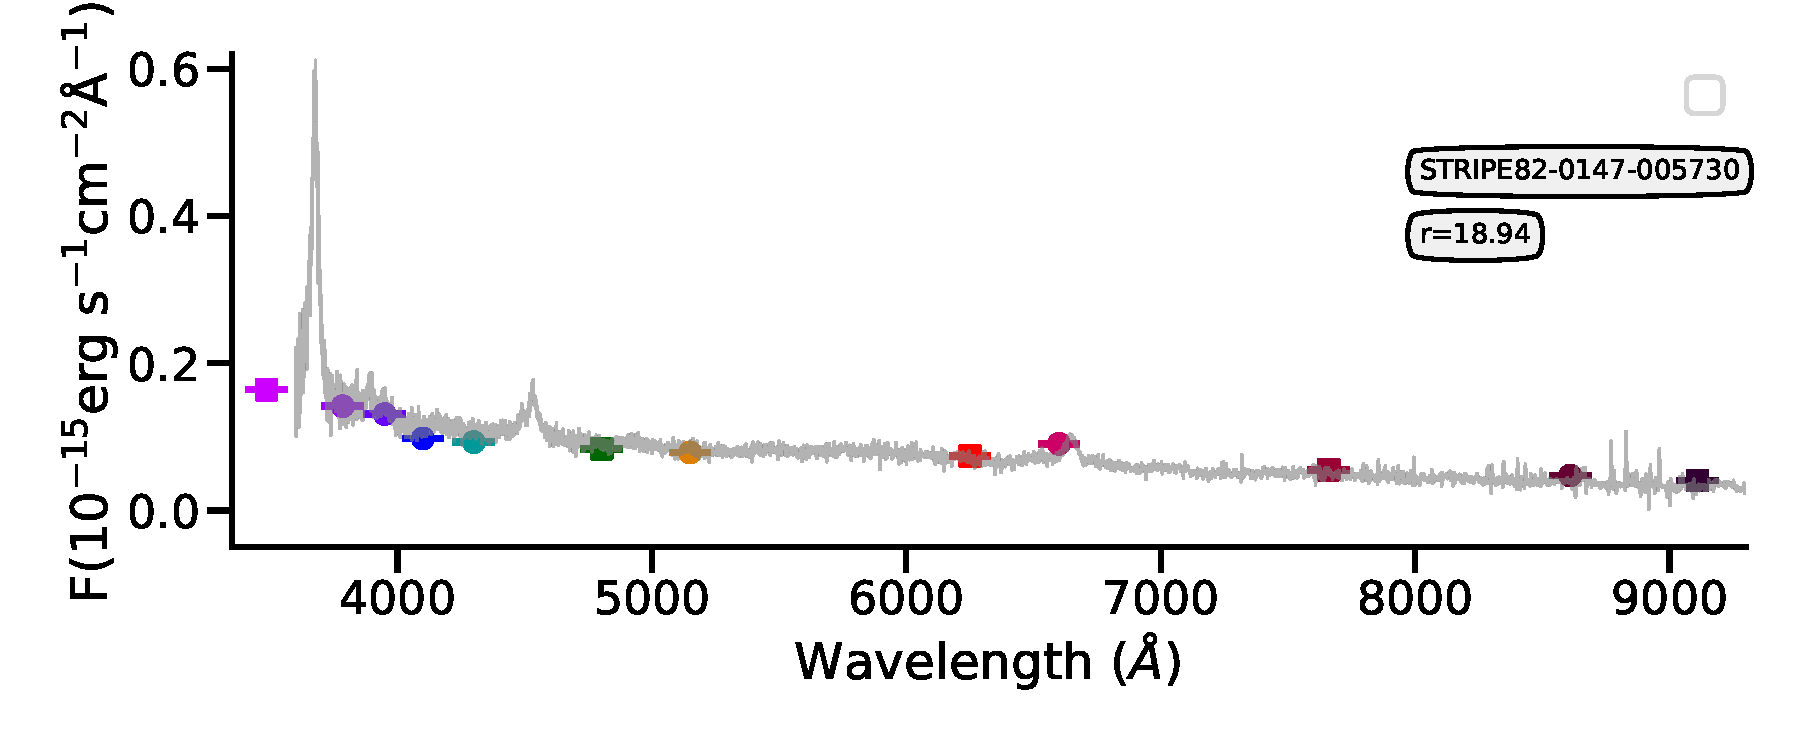
\includegraphics[trim=10 0 10 20, clip]{Figs/spec-9152-58041-0463-STRIPE82-0147-005730.pdf}
    & 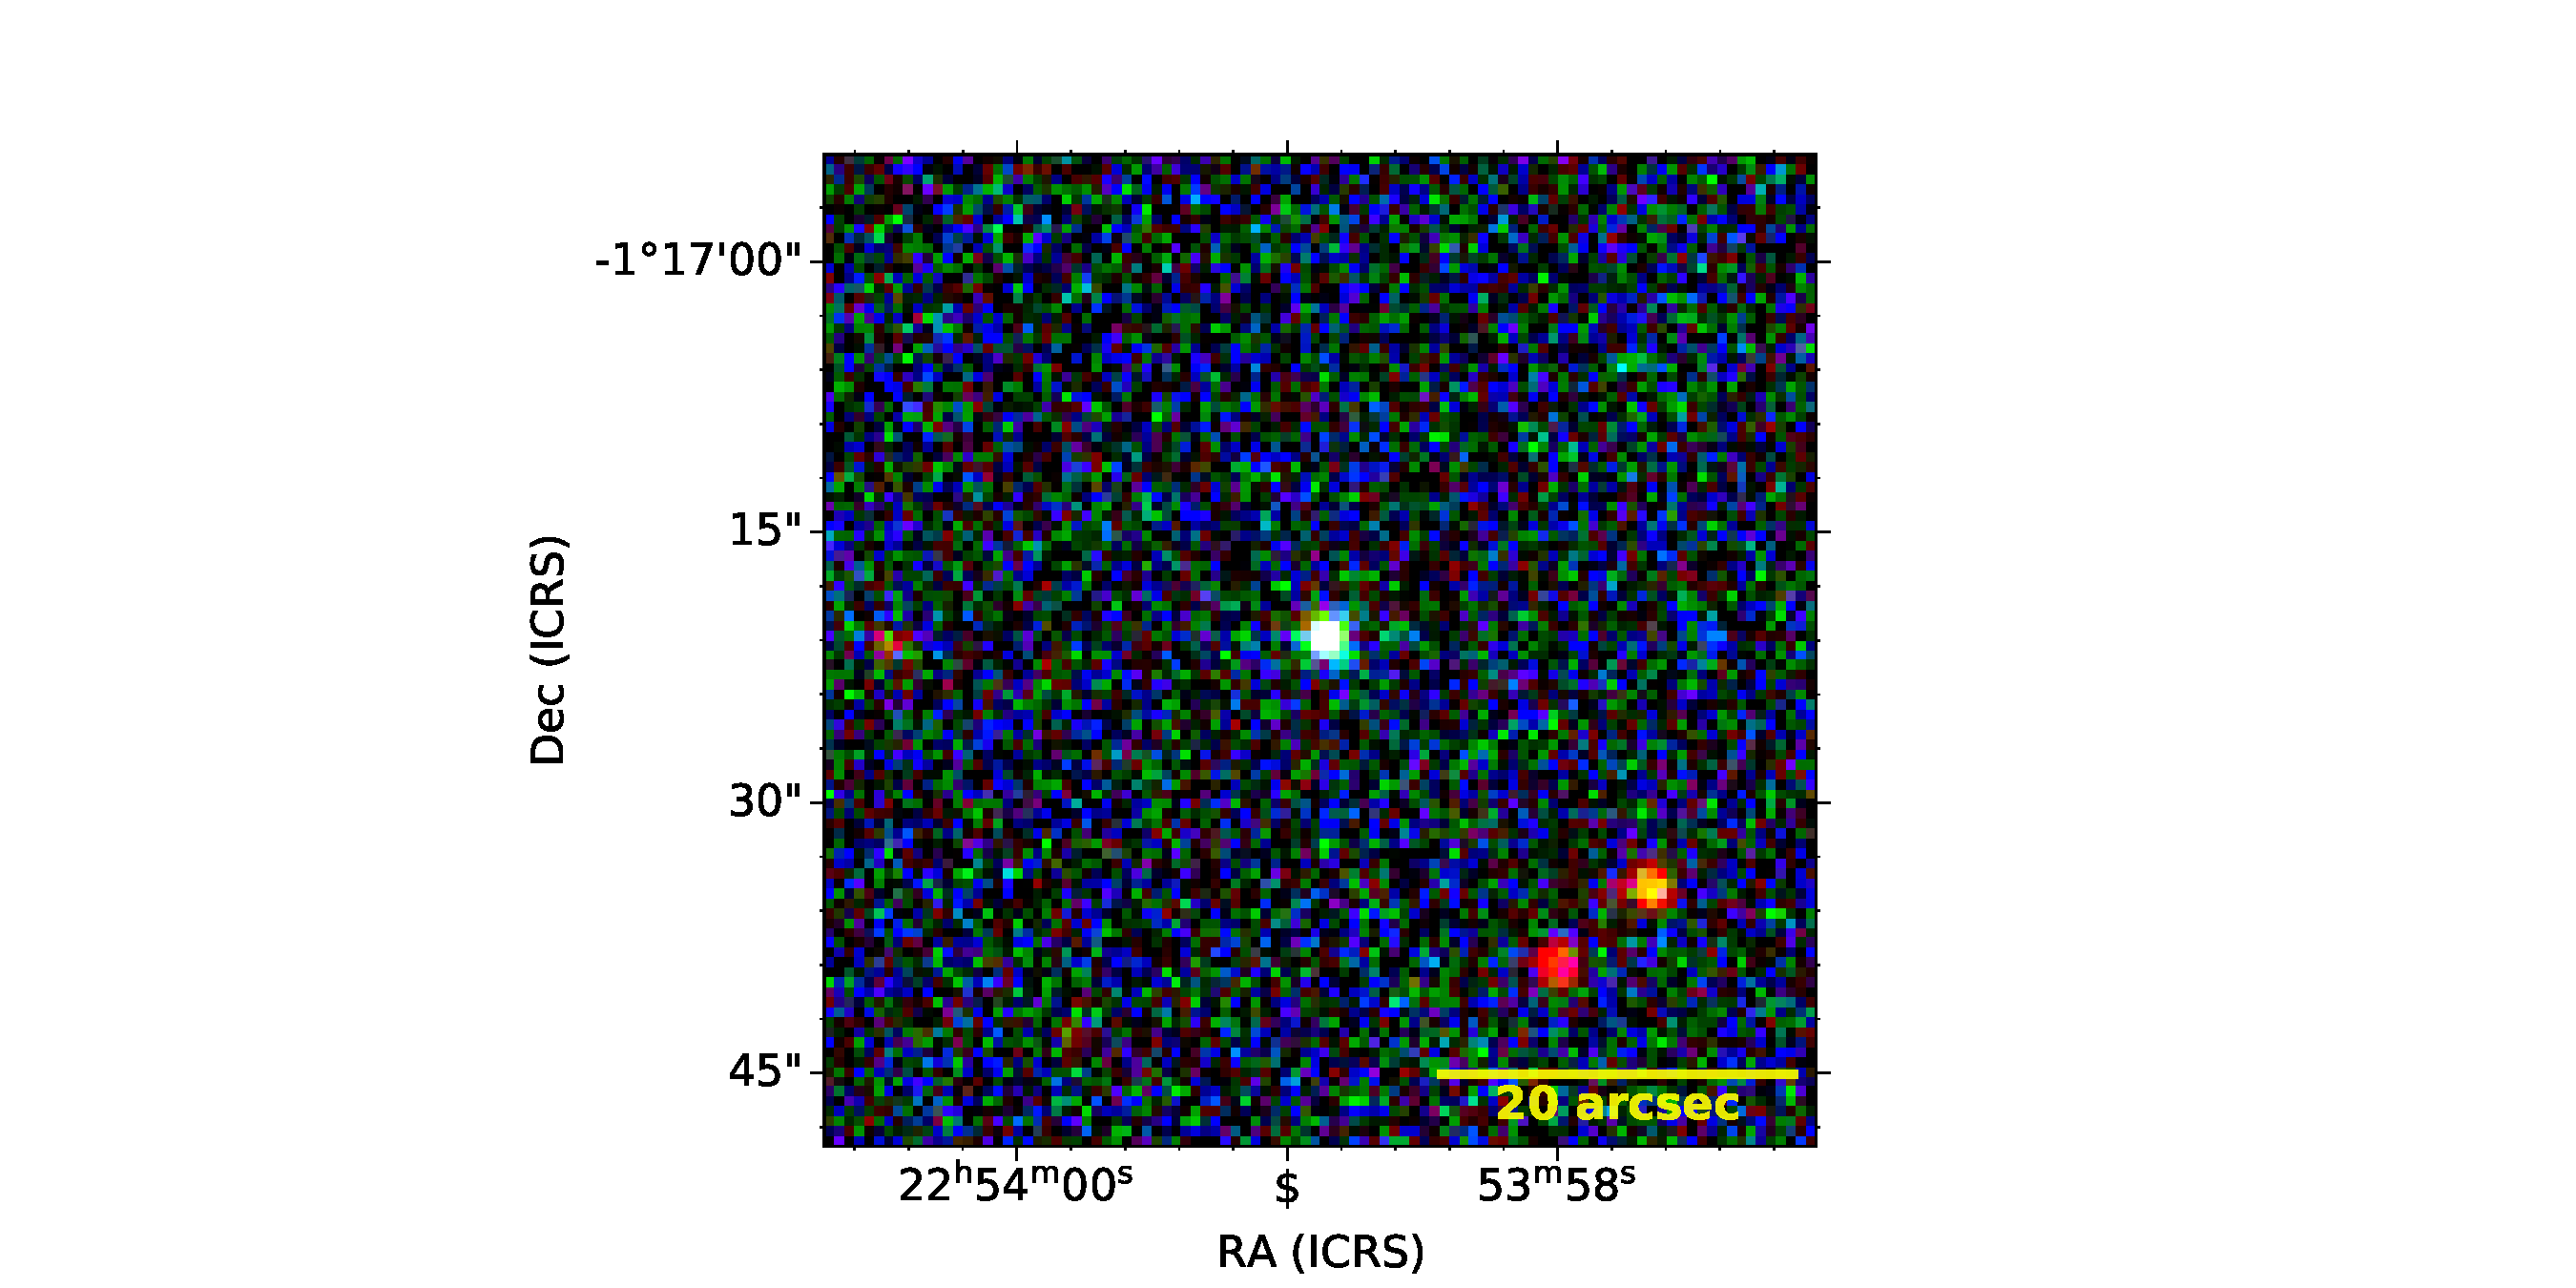
\includegraphics[width=0.4\linewidth, trim=10 0 10 20, clip]{Figs/STRIPE82-0147-005730_343-1_100_r.pdf} \\
    (c) & (d) \\
    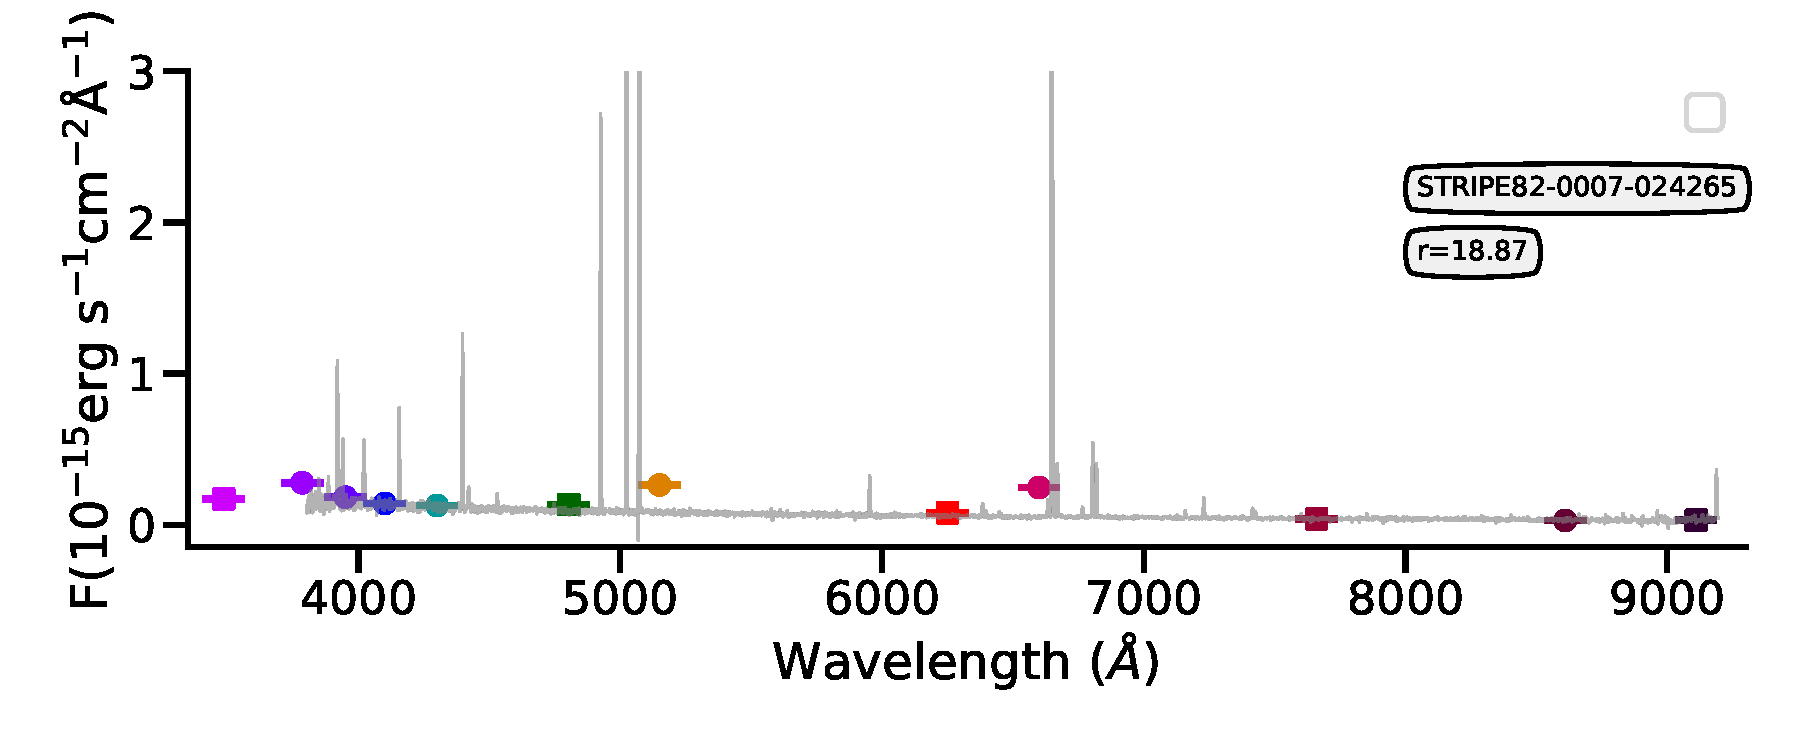
\includegraphics[trim=10 0 10 20, clip]{Figs/spec-1089-52913-0196-STRIPE82-0007-024265.pdf}
    & 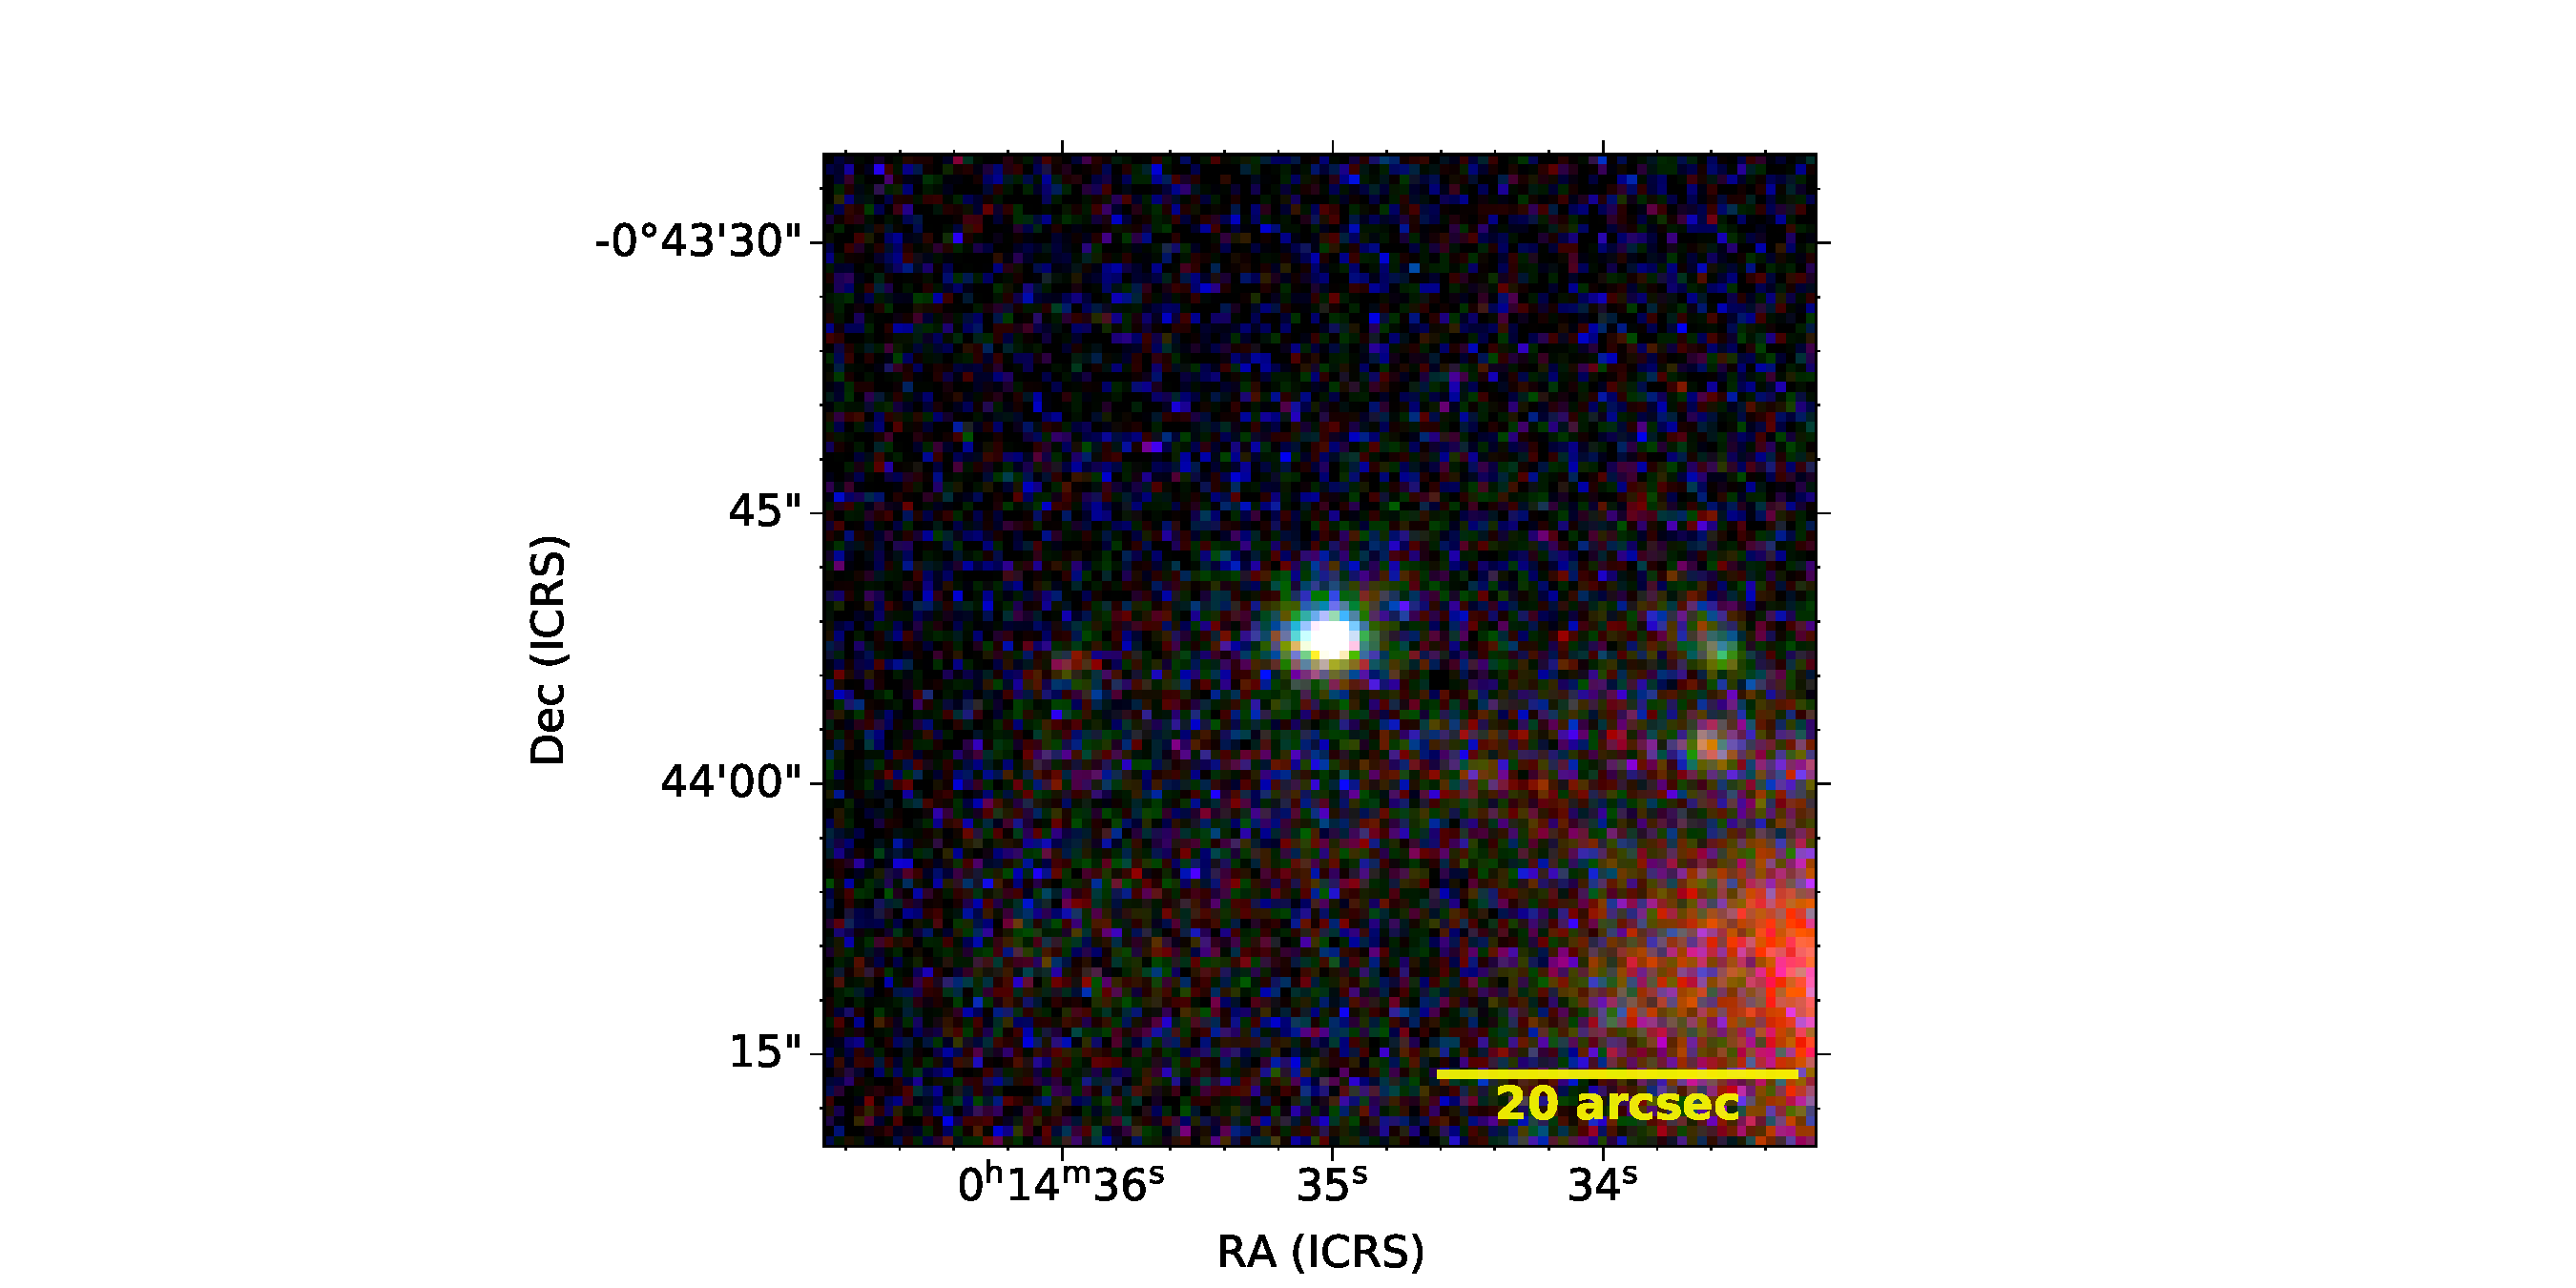
\includegraphics[width=0.4\linewidth, trim=10 0 10 20, clip]{Figs/STRIPE82-0007-024265_3-0_100_r.pdf} \\
  \end{tabular}
  \caption{Spectra of the SDSS}
  \label{fig:color-diagram}
\end{figure*}

\subsection{Magnitudes and color distributions}

\begin{figure}
  \begin{tabular}{l l l}
  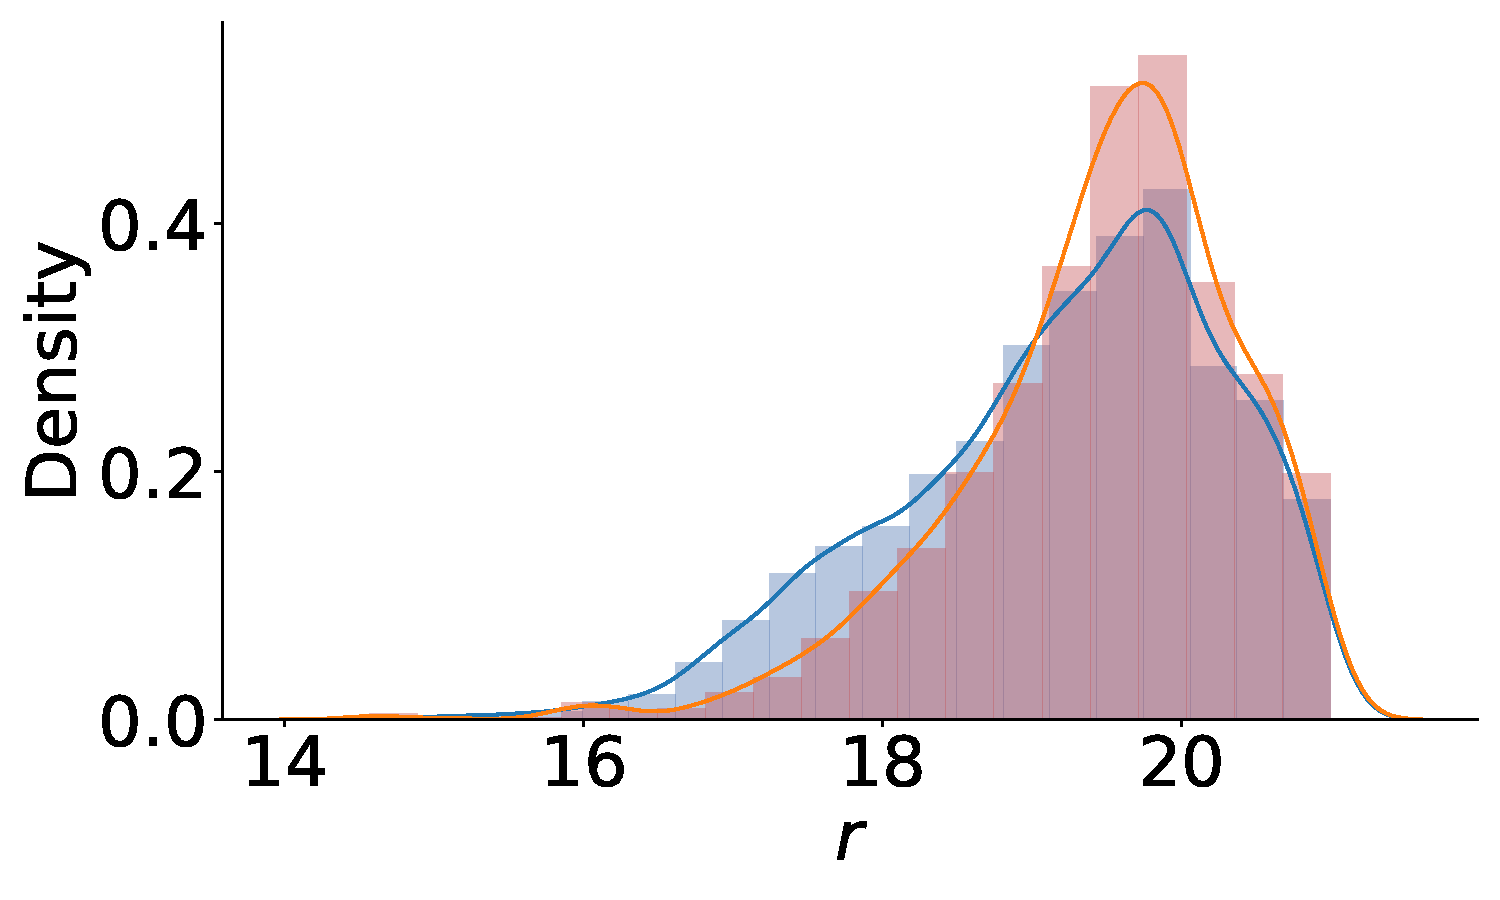
\includegraphics[width=\columnwidth]{Figs/distribution_r-group.pdf} \\
    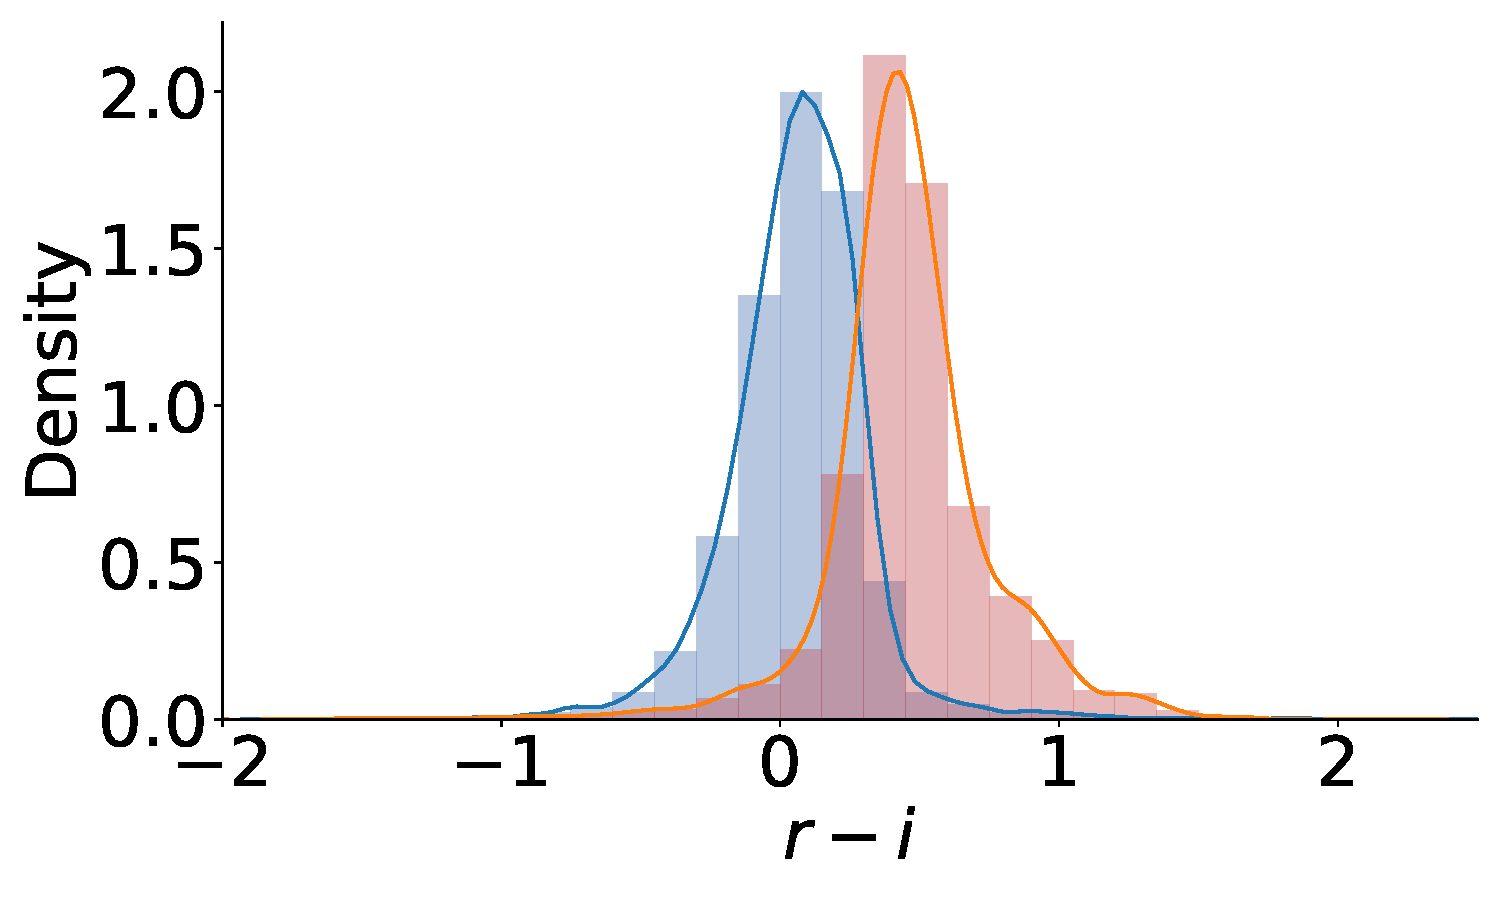
\includegraphics[width=\columnwidth]{Figs/distribution-ri-group.pdf}\\
    \includegraphics[width=\columnwidth]{Figs/distribution-Halpha-group.pdf}
  \end{tabular}
  \caption{Distribution of $r$ magnitude  (left panel), $(r - i)$ color (middle panel), and $(r - J0660)$
    color (right panel) for the blue and red sources of the sample of H$a\lpha$ emitters.
    Both sample are normalized to their maximum counts, xx and xx objects for blue and
    red sources, respectively.   The smooth curves represent a Kernel density estimation for both samṕles.}
    \label{fig:diagram-distri}
\end{figure}

Fig.~\ref{fig:diagram-distri} shows the magnitude and color distribution of the blue and red
sources --classification performed with machine learning on Section~\ref{sec:clustering}--.
Upper panel of the figure shows the distribution of the blue and red sources of the $r$ magnitude.
The peaks of the $r$ distribution is the same for the blue and red sources, which is around
$r \sim 19.9$. However, the density at the peak is higher in red sources than the blue ones
indicating that the proportion of objects with value $r$ of 19.9 is higher than the blue sources
The fraction of object is very small at $r < 16$ for each group of objects.
The distribution of the objects for both group increase in the range $16 \gtrsim r \gtrsim 19.9$.
However the density as indicating the Kernel density estimation curves is higher in the
blue sources. This implies that the fraction of sources with the magnitude range is considerable
higher in comparison with the red group. In conclusion the blue sources tends to be brighter
than the red ones.


Middle panel of figure displays the $(r - i)$ distribution of the blue and red emission line
objects. The peaks of the $(r - i)$ distributions are distinct for the blue and red sources.
The peaks of the red sources at high red continuum,  $(r - i) = 0.5$, compared to the value
of the blue sample, $(r - i) = -0.9$. All these results are consistent because the $(r - i)$
color is an indicating of reddened sources. This is also consistent with previous works,
since \citet{Wevers:2017} used different algorithms based on the  $(r - i)$ color
to successfully select blue outliers.

Botton panel of Fig.~\ref{fig:diagram-distri} shows the
$(r - J0660)$ color distribution of the blue and red objects.  The fraction of objects selected
as emitter rises drastically with $J$0660 excess, until at sufficiently large excesses. The peaks
of the $(r - J0660)$ color distribution are relatively different for both groups of sources.
Having the blue sources the peaks at  $(r - J0660) = 0.5$ while for the red one the value peak
is $(r - J0660)=0.7$.


\section{Conclusions}

We have created an usefully and important sample of emission line objects.
By identifying the locus of main-sequence and giant star and considering as
$J0660$-excess the objects that above of the locus, we have found
the emission line sources in S-PLUS DR3. In agreement with the results after
to find the coincidences with SIMBAD several type of emission objects are included
in our list which including nebulae, binary systems, stars, emission line galaxies,
quasars, globular clusters among other.

We also found that using the colors $g - r$ and $(z - g)$ is very efficient to separate
the blue sources from the red ones.

We also found that using this colors as the input to implement unsupervised machine learning
in better to group the source in the red or blue sources.

\section*{Acknowledgements}

The S-PLUS project, including the T80-South robotic telescope and
the S-PLUS scientific survey, was founded as a partnership between the
Fundação de Amparo à Pesquisa do Estado de S\~{a}o Paulo
(FAPESP), the Observatório Nacional (ON), the Federal University of
Sergipe (UFS), and the Federal University of Santa Catarina
(UFSC), with important financial and practical contributions from
other collaborating institutes in Brazil, Chile (Universidad de La
Serena), and Spain (Centro de Estudios de Física del Cosmos de
Aragón, CEFCA). We further acknowledge financial support from
the São Paulo Research Foundation (FAPESP), the Brazilian National
Research Council (CNPq), the Coordination for the Improvement of
Higher Education Personnel (CAPES), the Carlos Chagas Filho Rio
de Janeiro State Research Foundation (FAPERJ), and the Brazilian
Innovation Agency (FINEP).

Funding for the SDSS and SDSS-II has been provided by the Alfred P.
Sloan Foundation, the Participating Institutions, the National Science
Foundation, the U.S. Department of Energy, the National Aeronautics
and Space Administration, the Japanese Monbukagakusho, the Max
Planck Society, and the Higher Education Funding Council for England.
The SDSS Web Site is \url{http://www.sdss.org/}.

The SDSS is managed by the Astrophysical Research Consortium for
the Participating Institutions. The Participating Institutions
are the American Museum of Natural History, Astrophysical Institute Potsdam,
University of Basel, University of Cambridge, Case Western Reserve University,
University of Chicago, Drexel University, Fermilab, the Institute for Advanced
Study, the Japan Participation Group, Johns Hopkins University, the Joint
Institute for Nuclear Astrophysics, the Kavli Institute for Particle Astrophysics
and Cosmology, the Korean Scientist Group, the Chinese Academy of Sciences (LAMOST),
Los Alamos National Laboratory, the Max-Planck-Institute for Astronomy (MPIA),
the Max-Planck-Institute for Astrophysics (MPA), New Mexico State University,
Ohio State University, University of Pittsburgh, University of Portsmouth,
Princeton University, the United States Naval Observatory, and the University
of Washington.

Guoshoujing Telescope (the Large Sky Area Multi-Object Fiber Spectroscopic
Telescope LAMOST) is a National Major Scientific Project built by the Chinese
Academy of Sciences. Funding for the project has been provided by the National
Development and Reform Commission. LAMOST is operated and managed by the
National Astronomical Observatories, Chinese Academy of Sciences. 


%%%%%%%%%%%%%%%%%%%%%%%%%%%%%%%%%%%%%%%%%%%%%%%%%%
\section*{Data Availability}


%%%%%%%%%%%%%%%%%%%% REFERENCES %%%%%%%%%%%%%%%%%%

% The best way to enter references is to use BibTeX:

\bibliographystyle{mnras}
\bibliography{ref} 


%%%%%%%%%%%%%%%%%%%%%%%%%%%%%%%%%%%%%%%%%%%%%%%%%%

%%%%%%%%%%%%%%%%% APPENDICES %%%%%%%%%%%%%%%%%%%%%

\appendix
\section{Condensed Trees}
\label{sec:trees}

The question now is what does the cluster hierarchy look like - which
clusters are near each other, or could perhaps be merged, and which
are far apart. We can access the basic hierarchy via the \texttt{condensed\_tree\_}
attribute of the clusterer object. It is possible to see that \texttt{HDBSCAN} has found
two cluster that in agreement with previous results are the blue and red sources.

\begin{figure*}
	\includegraphics[width=0.9\linewidth]{Figs/cluster-hierarchy-hdbscan.pdf}
        \caption{Branches were selected by the HDBSCAN* algorithm.}
    \label{fig:treess}
\end{figure*}


\newcommand\TableHeader{
  \hline\hline
  Id Object & \(\mathrm{RA}\) & \(\mathrm{Dec}\) & Type & Redshift & Group & P(Blue) &  P(Red)\\
            &                 &                  &      &          &{\sc hac}& {\sc hdbscan}& {\sc hdbscan} \\
  %Object & \(D\) &   \(R_{\mathrm{out}}\) & \(R_{\mathrm{in}}\) \\
  \hline 
}

\clearpage
\section{Simbad objects}

\begin{center}
\begin{longtable}{lrrccccc}
  \caption{Simbad sources. \label{tab:simbad}}\\
  \TableHeader\endfirsthead 
  \caption[]{--continued}\\
  \TableHeader\endhead
  \hline \endfoot
%% \begin{table}
%% \begin{tabular}{ccccccc}
%% main_id & RA Sex & DEC Sex & main_type & Label_hier & P(Blue) & P(red) \\
CTLGD 9478 & 0:01:59.25 & -29:18:40.4 & Star & Blue & 0.98 & 0.01 \\
QSO B2359+005 & 0:02:30.71 & +0:49:59.2 & QSO & Blue & 0.73 & 0.07 \\
$[$GMB2011$]$ 1808 & 0:02:47.58 & -0:22:23.5 & ClG & -- & -- & -- \\
CTLGD 2037 & 0:05:08.77 & -30:51:04.2 & Star & Red & 0.14 & 0.73 \\
SDSS J000637.99-003656.2 & 0:06:37.99 & -0:36:56.2 & QSO & -- & -- & -- \\
LBQS 0004+0036 & 0:07:10.00 & +0:53:29.1 & QSO & Blue & 0.61 & 0.11 \\
SDSS J000809.34+004935.5 & 0:08:09.34 & +0:49:35.3 & QSO & -- & -- & -- \\
2SLAQ J000918.74-003907.2 & 0:09:18.76 & -0:39:07.0 & Galaxy & Blue & 0.70 & 0.07 \\
$[$VV2006$]$ J001040.1-294428 & 0:10:40.08 & -29:44:27.3 & QSO & Blue & 0.71 & 0.13 \\
CTLGD 7291 & 0:10:48.73 & -29:47:28.8 & Star & Red & 0.29 & 0.35 \\
2QZ J001055.3-304423 & 0:10:55.37 & -30:44:23.5 & Galaxy & Blue & 0.57 & 0.07 \\
$[$VV2006$]$ J001228.8-310241 & 0:12:28.78 & -31:02:40.0 & QSO & Blue & 0.48 & 0.07 \\
LBQS 0010+0035 & 0:13:27.32 & +0:52:32.2 & Seyfert 1 & Blue & 0.77 & 0.07 \\
$[$GPM2009$]$ J0014-0044 2 & 0:14:28.79 & -0:44:43.8 & EmG & Blue & 0.15 & 0.05 \\
2SLAQ J001455.99+001903.5 & 0:14:55.99 & +0:19:03.7 & Star & Blue & 0.78 & 0.06 \\
2SLAQ J001526.52+001813.2 & 0:15:26.52 & +0:18:13.4 & QSO & Blue & 0.50 & 0.08 \\
$[$VV2006$]$ J001535.5+005355 & 0:15:35.55 & +0:53:56.1 & QSO & Blue & 0.77 & 0.02 \\
SDSS J001628.25+010801.9 & 0:16:28.24 & +1:08:02.0 & Galaxy & Blue & 0.69 & 0.12 \\
$[$VV2006$]$ J001641.9-312657 & 0:16:41.87 & -31:26:56.6 & QSO & Blue & 0.74 & 0.09 \\
2SLAQ J001731.27-004859.3 & 0:17:31.26 & -0:48:59.2 & QSO & Blue & 0.75 & 0.10 \\
LEDA    1156 & 0:17:39.97 & +0:30:22.5 & StarburstG & Blue & 0.94 & 0.01 \\
SDSS J001753.82+005057.6 & 0:17:53.82 & +0:50:57.7 & QSO & -- & -- & -- \\
2SLAQ J001912.39+000319.6 & 0:19:12.39 & +0:03:19.8 & QSO & Blue & 0.74 & 0.07 \\
2SLAQ J001940.23-005435.9 & 0:19:40.24 & -0:54:35.8 & QSO & Blue & 0.69 & 0.04 \\
$[$VV2006$]$ J001950.1-004040 & 0:19:50.06 & -0:40:40.7 & QSO & -- & -- & -- \\
2SLAQ J002237.90+000519.0 & 0:22:37.90 & +0:05:19.2 & QSO & Blue & 0.55 & 0.02 \\
UM 240 & 0:25:07.40 & +0:18:45.2 & EmObj & Blue & 0.73 & 0.11 \\
2MASX J00251994+0031312 & 0:25:19.92 & +0:31:31.7 & Seyfert 1 & Blue & 0.82 & 0.03 \\
LEDA 3107905 & 0:27:53.84 & -0:58:00.2 & Galaxy & Blue & 0.96 & 0.02 \\
SDSS J002916.79-010021.5 & 0:29:16.81 & -1:00:23.1 & Galaxy & Blue & 1.0 & 3.22 \\
SDSS J002940.01+010528.5 & 0:29:40.02 & +1:05:28.7 & QSO & Blue & 0.55 & 0.04 \\
$[$VV2010c$]$ J002951.5+004159 & 0:29:51.45 & +0:42:00.0 & AGN & Red & 0.34 & 0.18 \\
SDSS J003117.70+001705.0 & 0:31:17.69 & +0:17:05.1 & QSO & -- & -- & -- \\
2QZ J003137.5-292815 & 0:31:37.50 & -29:28:15.3 & Unknown & Blue & 0.66 & 0.03 \\
2dFGRS TGS283Z142 & 0:31:50.70 & -28:55:36.7 & Galaxy & Blue & 0.89 & 0.01 \\
2QZ J003152.5-293534 & 0:31:52.56 & -29:35:33.3 & Galaxy & Blue & 0.86 & 0.06 \\
2SLAQ J003208.53-005303.7 & 0:32:08.53 & -0:53:03.6 & QSO & Blue & 0.36 & 0.06 \\
SDSS J003234.62-001557.1 & 0:32:34.62 & -0:15:57.1 & QSO & Blue & 0.40 & 0.08 \\
LEDA  559945 & 0:32:34.69 & -42:40:10.4 & Galaxy & Blue & 0.70 & 0.04 \\
$[$VV2006$]$ J003242.7+003111 & 0:32:42.74 & +0:31:11.1 & QSO & Blue & 0.21 & 0.06 \\
2dFGRS TGS365Z059 & 0:33:54.71 & -29:56:12.7 & Galaxy & Blue & 0.78 & 0.02 \\
SWIRE J003517.14-420518.6 & 0:35:17.11 & -42:05:19.0 & AGN & Red & 0.03 & 0.66 \\
$[$VV2006$]$ J003545.9+002306 & 0:35:45.86 & +0:23:06.0 & QSO & Blue & 0.81 & 0.02 \\
2MASS J00362543-0029075 & 0:36:25.39 & -0:29:07.1 & AGN & Red & 0.16 & 0.75 \\
2dFGRS TGS440Z027 & 0:36:38.44 & -32:34:44.7 & Galaxy & Blue & 0.28 & 0.07 \\
$[$VV2006$]$ J003714.1-005602 & 0:37:14.11 & -0:56:04.0 & QSO & -- & -- & -- \\
$[$VV2006$]$ J003722.2-001140 & 0:37:22.17 & -0:11:40.6 & QSO & Blue & 0.69 & 0.03 \\
UM 260 & 0:37:41.13 & +0:33:20.0 & EmObj & Blue & 0.69 & 0.07 \\
SDSS J003859.34-004252.2 & 0:38:59.35 & -0:42:52.0 & QSO & Blue & 0.11 & 0.04 \\
SDSS J003930.30+012021.6 & 0:39:30.28 & +1:20:20.9 & BlueCompG & Blue & 0.30 & 0.06 \\
IRAS 00370+0035 & 0:39:34.78 & +0:51:36.9 & FIR & Blue & 0.82 & 0.03 \\
IRAS 00370+0035 & 0:39:34.78 & +0:51:36.9 & FIR & Blue & 0.82 & 0.03 \\
2QZ J004215.6-321257 & 0:42:15.62 & -32:12:57.2 & Galaxy & Blue & 0.91 & 0.03 \\
GALEX 2673249256393934953 & 0:42:43.87 & +1:17:02.2 & QSO & Blue & 0.75 & 0.08 \\
2dFGRS TGS501Z235 & 0:43:21.88 & -33:19:02.9 & Galaxy & Blue & 0.57 & 0.14 \\
2SLAQ J004335.13-003729.7 & 0:43:35.16 & -0:37:29.6 & CataclyV* & Blue & 0.55 & 0.14 \\
SDSS J004415.83-004303.1 & 0:44:15.81 & -0:43:03.1 & QSO & -- & -- & -- \\
$[$VV2006$]$ J004544.4-315729 & 0:45:44.35 & -31:57:29.2 & QSO & Blue & 0.77 & 0.09 \\
2SLAQ J004626.30-011417.0 & 0:46:26.30 & -1:14:16.8 & Galaxy & Blue & 0.85 & 0.03 \\
$[$VV98$]$ J004826.9-341340 & 0:48:26.97 & -34:13:38.7 & QSO & Blue & 0.69 & 0.11 \\
SDSS J004918.52+011308.9 & 0:49:18.52 & +1:13:09.1 & QSO & Blue & 0.59 & 0.08 \\
LEDA    3034 & 0:51:49.42 & +0:33:53.8 & Seyfert 1 & Blue & 0.85 & 0.02 \\
QSO B0049-272 & 0:51:55.64 & -26:57:43.3 & QSO & Blue & 0.21 & 0.05 \\
$[$BKD2008$]$ WR 353 & 0:51:59.72 & -0:29:20.8 & PartofG & Blue & 0.54 & 0.07 \\
ESO 411-27 & 0:52:51.61 & -27:19:32.8 & Galaxy & Blue & 0.98 & 0.01 \\
SDSS J005343.78+012147.6 & 0:53:43.76 & +1:21:47.5 & QSO & Blue & 0.60 & 0.07 \\
RESOLVE rf554 & 0:54:15.54 & -1:04:56.0 & Galaxy & Blue & 0.97 & 0.02 \\
2QZ J005440.1-320042 & 0:54:40.12 & -32:00:42.2 & EmG & Blue & 0.56 & 0.03 \\
QSO B0052-307 & 0:54:43.95 & -30:30:54.1 & QSO & Blue & 0.67 & 0.09 \\
$[$VV2006$]$ J005532.1-311538 & 0:55:32.08 & -31:15:37.8 & QSO & Blue & 0.77 & 0.08 \\
$[$TYZ2012$]$ II  11 & 0:55:41.32 & -0:56:30.6 & Galaxy & Blue & 0.79 & 0.01 \\
$[$CT83$]$ 219 & 0:55:51.35 & -30:56:42.8 & UV & Blue & 0.58 & 0.07 \\
RGO  8439 & 0:55:53.16 & -28:54:57.3 & Star & Blue & 0.98 & 0.01 \\
2dFGRS TGS502Z028 & 0:55:53.31 & -33:39:01.5 & Galaxy & Blue & 0.69 & 0.14 \\
$[$VV2006$]$ J005609.9-312209 & 0:56:09.93 & -31:22:08.6 & QSO & Blue & 0.32 & 0.07 \\
$[$VV2006$]$ J005639.0-315759 & 0:56:39.05 & -31:57:58.6 & QSO & Blue & 1.0 & 6.38 \\
$[$GPM2009$]$ 0057-0022 & 0:57:12.60 & -0:21:57.7 & Galaxy & Blue & 0.77 & 0.12 \\
$[$VV2000$]$ J005840.5-300203 & 0:58:40.42 & -30:02:00.1 & QSO & Blue & 0.35 & 0.05 \\
LEDA    3530 & 0:59:04.10 & +1:00:04.2 & GinCl & Blue & 0.96 & 0.03 \\
2dFGRS TGS503Z245 & 0:59:13.57 & -34:19:15.7 & Galaxy & Blue & 0.96 & 0.03 \\
2MASX J00593609-3020390 & 0:59:36.09 & -30:20:39.0 & Galaxy & Red & 0.04 & 0.75 \\
LBQS 0057-0135 & 0:59:48.81 & -1:19:05.2 & QSO & Blue & 0.43 & 0.07 \\
QSO B0057-3948 & 0:59:53.21 & -39:31:57.3 & QSO & Blue & 0.84 & 0.04 \\
CAIRNS J005959.59-005157.2 & 0:59:59.58 & -0:51:57.1 & GinCl & Red & 7.11 & 1.0 \\
SCMS  679 & 1:00:04.44 & -33:39:32.5 & Star & Blue & 0.52 & 0.04 \\
2QZ J010009.9-320131 & 1:00:09.94 & -32:01:31.1 & Unknown & Blue & 0.99 & 0.00 \\
2dFGRS TGS561Z059 & 1:00:16.17 & -34:57:40.6 & Galaxy & Blue & 0.51 & 0.06 \\
2SLAQ J010121.76-000301.7 & 1:01:21.76 & -0:03:01.8 & Galaxy & Blue & 0.13 & 0.05 \\
QSO B0059-304B & 1:02:14.65 & -30:07:53.8 & QSO & Blue & 0.88 & 0.01 \\
2SLAQ J010230.03-003206.8 & 1:02:30.02 & -0:32:06.8 & Seyfert 1 & Blue & 0.50 & 0.08 \\
2MASX J01023175+0120363 & 1:02:31.78 & +1:20:36.1 & GinCl & Blue & 0.84 & 0.02 \\
$[$VV2006$]$ J010336.4-005508 & 1:03:36.39 & -0:55:08.8 & QSO & Blue & 0.54 & 0.06 \\
SDSS J010413.86-011552.1 & 1:04:13.86 & -1:15:52.0 & QSO & Blue & 0.96 & 0.03 \\
QSO B0103+00 & 1:06:19.23 & +0:48:23.4 & QSO & Red & 0.02 & 0.04 \\
6dFGS gJ010653.4-324342 & 1:06:53.44 & -32:43:41.9 & AGN & Blue & 0.63 & 0.02 \\
LIRAS J010658.95+010438.3 & 1:06:58.93 & +1:04:38.2 & AGN & Red & 0.12 & 0.73 \\
$[$VV2006$]$ J010705.6+000609 & 1:07:05.55 & +0:06:09.0 & QSO & Blue & 0.74 & 0.07 \\
UGC   695 & 1:07:46.47 & +1:03:50.3 & LSB G & Blue & 0.88 & 0.06 \\
SDSS J010748.62+004453.5 & 1:07:48.62 & +0:44:53.7 & BClG & Red & 0.13 & 0.43 \\
MCG+00-04-011 & 1:09:01.58 & +1:22:41.5 & GinCl & Blue & 0.73 & 0.06 \\
MCG+00-04-011 & 1:09:01.58 & +1:22:41.5 & GinCl & Blue & 0.73 & 0.06 \\
2SLAQ J010907.59+000649.8 & 1:09:07.59 & +0:06:50.0 & QSO & Blue & 0.54 & 0.06 \\
LEDA 1185205 & 1:09:07.95 & +1:07:15.5 & HII G & Blue & 0.74 & 0.13 \\
SDSS J010918.56+005419.3 & 1:09:18.56 & +0:54:19.4 & QSO & Blue & 0.64 & 0.08 \\
2SLAQ J010925.95-003739.0 & 1:09:25.96 & -0:37:39.0 & QSO & Blue & 0.69 & 0.03 \\
2QZ J011014.0-302445 & 1:10:13.97 & -30:24:44.5 & EmG & Blue & 0.59 & 0.04 \\
2QZ J011119.0-300019 & 1:11:19.02 & -30:00:18.2 & EmG & Blue & 0.83 & 0.05 \\
SDSS J011128.38+000143.7 & 1:11:28.35 & +0:01:43.3 & QSO & Blue & 0.13 & 0.10 \\
2dFGRS TGS505Z356 & 1:12:12.64 & -33:56:31.1 & Galaxy & Red & 0.43 & 0.13 \\
2SLAQ J011230.55+001441.5 & 1:12:30.55 & +0:14:41.7 & QSO & Blue & 0.83 & 0.03 \\
PB  6318 & 1:12:58.01 & +0:58:37.0 & Star & Blue & 0.64 & 0.04 \\
2dFGRS TGS447Z027 & 1:13:13.03 & -32:26:09.9 & Galaxy & Blue & 0.85 & 0.04 \\
UGC   772 & 1:13:40.42 & +0:52:39.0 & LSB G & -- & -- & -- \\
2SLAQ J011402.35-004750.9 & 1:14:02.35 & -0:47:50.8 & Seyfert 1 & Blue & 0.55 & 0.06 \\
$[$VV2006$]$ J011405.3-310903 & 1:14:05.25 & -31:09:02.8 & QSO & Blue & 0.21 & 0.04 \\
2dFGRS TGS505Z120 & 1:14:36.11 & -32:38:41.0 & Galaxy & Blue & 0.79 & 0.08 \\
SDSS J011531.90-005144.5 & 1:15:31.89 & -0:51:44.3 & HII G & Blue & 0.89 & 0.05 \\
2SLAQ J011533.07-005134.9 & 1:15:33.06 & -0:51:34.8 & Galaxy & Blue & 0.56 & 0.07 \\
$[$BKD2008$]$ WR 354 & 1:15:33.79 & -0:51:31.5 & HII G & Blue & 0.22 & 0.07 \\
$[$BKD2008$]$ WR 354 & 1:15:33.79 & -0:51:31.5 & HII G & Blue & 0.22 & 0.07 \\
2SLAQ J011542.18+002300.2 & 1:15:42.18 & +0:23:00.4 & QSO & Blue & 0.68 & 0.04 \\
2dFGRS TGS505Z064 & 1:16:38.40 & -32:55:39.1 & Galaxy & Blue & 0.94 & 0.01 \\
2dFGRS TGS505Z018 & 1:17:40.21 & -33:04:40.7 & Galaxy & Blue & 0.67 & 0.07 \\
2dFGRS TGS377Z137 & 1:17:56.44 & -30:26:25.8 & Galaxy & Blue & 0.86 & 0.08 \\
2dFGRS TGS506Z276 & 1:18:05.71 & -33:03:09.1 & Galaxy & Blue & 0.88 & 0.06 \\
2SLAQ J011818.13+001455.2 & 1:18:18.12 & +0:14:55.5 & QSO & Blue & 0.62 & 0.03 \\
2SLAQ J011829.63+004549.4 & 1:18:29.62 & +0:45:49.4 & Seyfert 1 & Blue & 0.67 & 0.13 \\
2dFGRS TGS506Z243 & 1:18:49.15 & -33:20:13.1 & Galaxy & Blue & 0.83 & 0.07 \\
2MASX J01195427-3414599 & 1:19:54.23 & -34:15:00.0 & EmG & Blue & 0.98 & 0.01 \\
2dFGRS TGS506Z158 & 1:20:09.99 & -33:14:10.7 & Galaxy & Blue & 0.99 & 0.00 \\
2SLAQ J012110.74-005037.2 & 1:21:10.74 & -0:50:37.1 & QSO & Blue & 0.71 & 0.02 \\
$[$HB93$]$ 0119-341B & 1:21:52.19 & -33:56:15.8 & Star & Red & 0.33 & 0.18 \\
SDSS J012213.85+005731.4 & 1:22:13.87 & +0:57:31.6 & HII G & Blue & 1.0 & 3.25 \\
2dFGRS TGS565Z149 & 1:22:17.09 & -34:02:41.6 & Galaxy & Blue & 0.87 & 0.04 \\
2SLAQ J012226.76+000327.5 & 1:22:26.75 & +0:03:27.9 & QSO & Blue & 0.85 & 0.04 \\
QSO B0120-002 & 1:23:01.78 & +0:03:23.6 & QSO & Blue & 0.80 & 0.08 \\
2dFGRS TGS297Z222 & 1:23:50.87 & -29:11:46.4 & Galaxy & Blue & 0.05 & 0.02 \\
MCG+00-04-113 & 1:23:54.75 & +0:16:56.4 & GinCl & Blue & 0.70 & 0.04 \\
SDSS J012356.34+001230.6 & 1:23:56.35 & +0:12:31.0 & Galaxy & Blue & 0.99 & 0.00 \\
ESO 352-67 & 1:23:57.47 & -33:48:07.5 & Galaxy & Blue & 0.89 & 0.05 \\
SDSS J012405.73+005905.0 & 1:24:05.73 & +0:59:04.9 & Galaxy & -- & -- & -- \\
QSO B0121-324 & 1:24:16.18 & -32:12:21.7 & QSO & Blue & 0.61 & 0.07 \\
2dFGRS TGS507Z113 & 1:24:30.16 & -33:38:45.5 & Galaxy & Red & 0.44 & 0.39 \\
QSO B0122-3232 & 1:25:04.59 & -32:17:14.6 & QSO & Blue & 0.40 & 0.08 \\
2QZ J012526.2-304433 & 1:25:26.24 & -30:44:32.8 & EmG & Blue & 0.56 & 0.06 \\
2QZ J012549.3-280944 & 1:25:49.29 & -28:09:43.6 & Galaxy & -- & -- & -- \\
LEDA 1180903 & 1:26:27.03 & +0:58:51.9 & Galaxy & Blue & 0.97 & 0.02 \\
2dFGRS TGS566Z338 & 1:26:37.73 & -34:35:13.8 & Galaxy & Blue & 0.88 & 0.01 \\
6dFGS gJ012646.5-003845 & 1:26:46.51 & -0:38:44.7 & HII G & Blue & 0.54 & 0.07 \\
ESO 413-7 & 1:27:59.31 & -29:05:12.0 & GinCl & Blue & 1.0 & 3.24 \\
6dFGS gJ012926.6-011159 & 1:29:26.54 & -1:11:59.0 & GinCl & Red & 0.41 & 0.23 \\
SDSS J013034.18-002106.6 & 1:30:34.17 & -0:21:06.5 & QSO & Blue & 0.64 & 0.03 \\
2dFGRS TGS509Z295 & 1:31:21.84 & -33:06:06.2 & Galaxy & Blue & 0.81 & 0.06 \\
2dFGRS TGS508Z142 & 1:31:45.65 & -32:56:56.8 & Galaxy & Blue & 0.95 & 0.02 \\
LEDA  679811 & 1:31:47.24 & -33:10:55.1 & Galaxy & Blue & 0.99 & 0.00 \\
2dFGRS TGS509Z242 & 1:32:53.43 & -33:26:42.7 & Galaxy & Blue & 0.61 & 0.11 \\
2MASS J01330450+0003553 & 1:33:04.52 & +0:03:56.1 & low-mass* & Red & 0.13 & 0.47 \\
2SLAQ J013400.41-010358.2 & 1:34:00.46 & -1:03:59.2 & Galaxy & Blue & 0.99 & 0.00 \\
RESOLVE rf246 & 1:34:52.04 & -0:38:55.2 & Galaxy & Blue & 0.66 & 0.12 \\
$[$VV2006$]$ J013500.8-004054 & 1:35:00.83 & -0:40:54.2 & QSO & Blue & 0.16 & 0.04 \\
FBQS J0135-0019 & 1:35:17.53 & -0:19:39.0 & Seyfert 1 & Blue & 0.45 & 0.10 \\
2QZ J013531.1-313651 & 1:35:31.16 & -31:36:51.0 & Galaxy & Blue & 0.45 & 0.07 \\
SDSS J013701.72-012059.3 & 1:37:01.71 & -1:20:59.1 & QSO & Blue & 0.85 & 0.06 \\
$[$VV2006$]$ J013729.4-320715 & 1:37:29.40 & -32:07:15.7 & QSO & Blue & 0.55 & 0.04 \\
$[$VV2006$]$ J013837.3+002818 & 1:38:37.28 & +0:28:18.5 & QSO & Blue & 0.81 & 0.07 \\
2SLAQ J013951.07+002537.9 & 1:39:51.07 & +0:25:38.0 & QSO & Blue & 0.96 & 0.03 \\
2E   458 & 1:40:17.06 & -0:50:03.0 & Seyfert 1 & Blue & 0.26 & 0.05 \\
SDSS J014125.63+000755.6 & 1:41:25.64 & +0:07:55.8 & QSO & Red & 0.03 & 0.85 \\
$[$VV2006$]$ J014224.7-320414 & 1:42:24.73 & -32:04:13.7 & QSO & Blue & 0.54 & 0.09 \\
$[$VV2006$]$ J014303.6-295255 & 1:43:03.49 & -29:52:54.8 & QSO & Blue & 0.44 & 0.07 \\
ESO 353-36 & 1:43:18.29 & -34:12:22.4 & EmG & Red & 0.06 & 0.36 \\
SDSS J014721.12-004505.3 & 1:47:21.12 & -0:45:05.3 & QSO & Red & 0.33 & 0.35 \\
$[$VV2006$]$ J014739.2-285259 & 1:47:39.21 & -28:52:59.2 & QSO & Blue & 0.75 & 0.05 \\
$[$VV2006$]$ J014739.2-285259 & 1:47:39.21 & -28:52:59.3 & QSO & Blue & 0.84 & 0.04 \\
SDSS J014806.25-002841.6 & 1:48:06.25 & -0:28:41.6 & Galaxy & Blue & 0.70 & 0.04 \\
$[$VV2006$]$ J014812.2+000154 & 1:48:12.24 & +0:01:53.5 & QSO & Blue & 0.06 & 0.02 \\
2QZ J014844.1-275610 & 1:48:44.17 & -27:56:11.0 & Star & Blue & 0.72 & 0.06 \\
IC 1734 & 1:49:17.03 & -32:44:33.1 & Galaxy & Blue & 0.59 & 0.06 \\
$[$VV2006$]$ J014921.5-003220 & 1:49:21.53 & -0:32:20.9 & QSO & Blue & 0.80 & 0.07 \\
$[$RGD2013$]$ J015239.744+010557.768 & 1:52:39.74 & +1:05:57.9 & Galaxy & Red & 0.15 & 0.62 \\
$[$RGD2013$]$ J015253.854+011215.480 & 1:52:53.85 & +1:12:15.5 & Galaxy & Red & 0.04 & 0.87 \\
2QZ J015257.7-284838 & 1:52:57.76 & -28:48:37.8 & Seyfert 1 & Blue & 0.51 & 0.08 \\
2SLAQ J015331.85+002252.8 & 1:53:31.85 & +0:22:53.0 & QSO & Blue & 0.91 & 0.01 \\
SDSS J015400.48-004509.5 & 1:54:00.50 & -0:45:10.0 & HII G & Blue & 0.66 & 0.04 \\
2SLAQ J015409.27+002645.2 & 1:54:09.27 & +0:26:45.3 & QSO & Blue & 0.71 & 0.05 \\
$[$VV2006$]$ J015410.9-285214 & 1:54:10.94 & -28:52:14.6 & QSO & Blue & 0.54 & 0.06 \\
$[$VV2006$]$ J015415.4-285254 & 1:54:15.48 & -28:52:54.9 & QSO & Blue & 0.60 & 0.06 \\
SDSS J015440.44-000643.9 & 1:54:40.45 & -0:06:43.6 & EmG & Blue & 0.34 & 0.07 \\
2SLAQ J015526.89+000615.4 & 1:55:26.87 & +0:06:15.8 & Galaxy & Blue & 0.79 & 0.01 \\
2SLAQ J015529.12-003927.3 & 1:55:29.07 & -0:39:27.1 & Galaxy & Blue & 0.69 & 0.07 \\
SDSS J015813.75+010143.5 & 1:58:13.75 & +1:01:43.4 & RRLyr & Blue & 0.93 & 0.01 \\
$[$VV2006$]$ J015832.1-301703 & 1:58:32.15 & -30:17:02.8 & QSO & Blue & 0.75 & 0.09 \\
$[$VV2006$]$ J015832.1-301703 & 1:58:32.16 & -30:17:02.7 & QSO & Blue & 0.60 & 0.03 \\
$[$VV2006$]$ J015850.2-300438 & 1:58:50.22 & -30:04:38.1 & QSO & -- & -- & -- \\
$[$VV2006$]$ J015935.4+000401 & 1:59:35.48 & +0:04:01.5 & QSO & Blue & 0.62 & 0.07 \\
SDSS J020025.40+002916.5 & 2:00:25.40 & +0:29:16.8 & QSO & Red & 0.04 & 0.67 \\
$[$VV2006$]$ J020055.0-293527 & 2:00:55.02 & -29:35:26.5 & QSO & Blue & 0.63 & 0.04 \\
ESO 414-22 & 2:01:14.49 & -31:43:42.9 & GinGroup & Blue & 0.66 & 0.09 \\
$[$VV98$]$ J020115.4+003136 & 2:01:15.53 & +0:31:35.1 & QSO & Blue & 0.33 & 0.05 \\
2SLAQ J020200.06-000921.2 & 2:02:00.06 & -0:09:21.2 & QSO & Blue & 0.58 & 0.04 \\
$[$VV96$]$ J020435.5-455923 & 2:04:35.46 & -45:59:24.0 & QSO & Blue & 0.72 & 0.04 \\
LEDA 1193771 & 2:05:00.83 & +1:24:03.7 & Galaxy & Blue & 0.58 & 0.06 \\
2dFGRS TGS514Z164 & 2:07:20.33 & -33:01:54.3 & Galaxy & -- & -- & -- \\
2SLAQ J020804.48-000023.2 & 2:08:04.49 & -0:00:23.0 & QSO & Blue & 0.52 & 0.04 \\
2SLAQ J020827.06-005208.1 & 2:08:27.07 & -0:52:07.9 & QSO & Blue & 0.76 & 0.06 \\
SDSS J020921.99-005455.5 & 2:09:22.00 & -0:54:55.4 & QSO & Blue & 0.96 & 0.03 \\
2dFGRS TGS515Z070 & 2:12:25.05 & -33:04:59.0 & Galaxy & -- & -- & -- \\
2dFGRS TGS515Z311 & 2:14:24.22 & -33:14:52.0 & Galaxy & Blue & 0.86 & 0.08 \\
2dFGRS TGS461Z092 & 2:14:47.63 & -32:42:35.2 & Galaxy & Blue & 0.81 & 0.05 \\
2SLAQ J021529.02-005314.8 & 2:15:29.02 & -0:53:14.9 & QSO & Blue & 0.63 & 0.04 \\
2dFGRS TGS460Z130 & 2:16:01.62 & -31:36:51.8 & Galaxy & Blue & 0.91 & 0.02 \\
2dFGRS TGS387Z025 & 2:16:13.75 & -30:50:56.8 & Galaxy & Blue & 1.0 & 3.26 \\
SDSS J021617.19-011046.9 & 2:16:17.19 & -1:10:46.7 & QSO & Blue & 0.96 & 0.01 \\
2SLAQ J021810.52-010147.4 & 2:18:10.52 & -1:01:47.2 & QSO & Blue & 0.67 & 0.06 \\
V* AX For & 2:19:28.00 & -30:45:46.0 & CataclyV* & Blue & 0.45 & 0.06 \\
2QZ J022112.5-302559 & 2:21:12.54 & -30:25:59.0 & EmG & Blue & 0.80 & 0.07 \\
2SLAQ J022316.91-010049.7 & 2:23:16.93 & -1:00:49.6 & Galaxy & Blue & 0.85 & 0.05 \\
SHOC 120 & 2:24:17.14 & +0:06:26.1 & Seyfert 1 & -- & -- & -- \\
LEDA  667000 & 2:24:52.74 & -34:06:34.3 & Galaxy & Blue & 0.77 & 0.05 \\
SDSS J022530.93-005007.0 & 2:25:30.92 & -0:50:07.1 & Galaxy & Blue & 0.61 & 0.06 \\
$[$BKD2008$]$ WR 346 & 2:26:28.28 & +1:09:37.6 & PartofG & Blue & 0.99 & 0.00 \\
$[$BKD2008$]$ WR 346 & 2:26:28.28 & +1:09:37.6 & PartofG & Blue & 0.99 & 0.00 \\
LEDA  546974 & 2:26:46.27 & -43:35:29.6 & Galaxy & Blue & 0.64 & 0.07 \\
SDSS J022714.48+010536.1 & 2:27:14.47 & +1:05:36.3 & EmG & Blue & 0.65 & 0.07 \\
RESOLVE rf668 & 2:27:19.29 & +1:01:32.2 & Galaxy & Blue & 0.97 & 0.01 \\
$[$VV2006$]$ J022738.3-313627 & 2:27:38.28 & -31:36:26.4 & QSO & Blue & 0.45 & 0.06 \\
$[$VV2006$]$ J022758.2+000226 & 2:27:58.20 & +0:02:25.6 & QSO & -- & -- & -- \\
LCRS B022613.7-392927 & 2:28:14.52 & -39:16:04.0 & Galaxy & Blue & 0.67 & 0.04 \\
$[$BKD2008$]$ WR 315 & 2:28:28.73 & -1:08:58.6 & PartofG & Blue & 0.91 & 0.01 \\
2SLAQ J022945.34+000856.2 & 2:29:45.34 & +0:08:56.4 & Star & Blue & 0.53 & 0.08 \\
2QZ J022954.6-303558 & 2:29:54.69 & -30:35:58.4 & Seyfert 1 & Blue & 0.34 & 0.06 \\
Pul -3  180355 & 2:29:57.00 & -1:00:32.3 & Star & Red & 0.03 & 0.06 \\
2dFGRS TGS463Z130 & 2:30:09.77 & -31:36:18.2 & Galaxy & Blue & 0.99 & 0.00 \\
SDSS J023020.93+001355.5 & 2:30:20.93 & +0:13:55.8 & Seyfert 1 & Blue & 0.20 & 0.05 \\
UGC  2009 & 2:32:09.34 & -1:23:10.3 & Galaxy & Red & 0.02 & 0.87 \\
2dFGRS TGS518Z089 & 2:32:18.08 & -33:50:43.0 & Galaxy & Blue & 0.58 & 0.13 \\
SDSS J023230.63-011654.5 & 2:32:30.63 & -1:16:54.5 & QSO & Blue & 0.60 & 0.04 \\
6dFGS gJ023241.8-391744 & 2:32:41.88 & -39:17:42.8 & Galaxy & Blue & 0.50 & 0.08 \\
SDSS J023248.71+005138.8 & 2:32:48.71 & +0:51:38.8 & Galaxy & Blue & 0.56 & 0.06 \\
V* HP Cet & 2:33:22.62 & +0:50:59.4 & Nova & Blue & 0.54 & 0.08 \\
NGC   986 & 2:33:34.29 & -39:02:40.9 & EmG & Blue & 0.92 & 0.07 \\
$[$VV2006$]$ J023335.4-010744 & 2:33:35.37 & -1:07:44.6 & QSO & Blue & 0.50 & 0.06 \\
SDSS J023628.77-005829.7 & 2:36:28.75 & -0:58:30.0 & Galaxy & Blue & 0.77 & 0.08 \\
$[$VV2006$]$ J023635.7-003203 & 2:36:35.69 & -0:32:03.4 & QSO & -- & -- & -- \\
SDSS J024059.15+004545.8 & 2:40:59.14 & +0:45:45.9 & QSO & Blue & 0.98 & 0.01 \\
$[$VV2006$]$ J024235.0-010351 & 2:42:34.91 & -1:03:51.9 & QSO & Blue & 0.56 & 0.03 \\
$[$EKS96$]$ NGC 1068  91 & 2:42:46.94 & +0:01:26.2 & HII & Blue & 0.13 & 0.06 \\
$[$ZBF2015$]$ NGC1073   1 & 2:43:35.61 & +1:22:37.9 & HII & Blue & 0.27 & 0.06 \\
$[$ZBF2015$]$ NGC1073  16 & 2:43:37.69 & +1:22:22.5 & HII & Blue & 0.94 & 0.05 \\
$[$ZBF2015$]$ NGC1073  21 & 2:43:42.74 & +1:21:34.4 & HII & Blue & 0.50 & 0.07 \\
$[$ZBF2015$]$ NGC1073  10 & 2:43:44.03 & +1:22:40.5 & HII & Blue & 0.79 & 0.04 \\
6dFGS gJ024605.3-330500 & 2:46:05.28 & -33:04:59.4 & Galaxy & Blue & 0.82 & 0.01 \\
2MASS J02462415-0029539 & 2:46:24.14 & -0:29:52.9 & Star & Blue & 0.76 & 0.02 \\
Gaia DR2 2497764348684940160 & 2:46:24.75 & -0:30:16.3 & QSO & Blue & 0.53 & 0.06 \\
$[$BKD2008$]$ WR 316 & 2:46:25.42 & -0:30:09.8 & PartofG & Blue & 0.56 & 0.04 \\
2SLAQ J024626.59-003000.2 & 2:46:26.57 & -0:30:00.4 & Star & Blue & 0.99 & 0.00 \\
2SLAQ J025100.64+001707.2 & 2:51:00.64 & +0:17:07.3 & QSO & Blue & 0.69 & 0.06 \\
2SLAQ J025216.75+001741.2 & 2:52:16.73 & +0:17:41.2 & Galaxy & Blue & 0.88 & 0.06 \\
2SLAQ J025252.02-002211.7 & 2:52:52.00 & -0:22:11.6 & QSO & Blue & 0.85 & 0.04 \\
SHOC 143 & 2:54:26.13 & -0:41:22.7 & Seyfert 1 & Blue & 0.87 & 0.07 \\
NVSS J025557+004132 & 2:55:57.24 & +0:41:33.5 & RadioG & Red & 0.11 & 0.31 \\
QSO B0253+0058 & 2:56:07.25 & +1:10:38.8 & QSO & Blue & 0.65 & 0.07 \\
HBQS 0253+0022 & 2:56:25.32 & +0:34:29.4 & HII & Blue & 0.99 & 0.00 \\
LEDA 1170514 & 2:56:28.43 & +0:36:28.2 & Galaxy & Blue & 0.63 & 0.04 \\
2dFGRS TGS522Z138 & 2:57:45.54 & -33:28:55.5 & Galaxy & Red & 0.43 & 0.28 \\
2MASSI J0259103-002239 & 2:59:10.38 & -0:22:39.8 & Seyfert 1 & Blue & 0.53 & 0.08 \\
2SLAQ J030309.82+001337.5 & 3:03:09.83 & +0:13:37.8 & Galaxy & -- & -- & -- \\
UGC  2517 & 3:04:12.47 & -1:11:33.8 & Galaxy & Red & 0.53 & 0.19 \\
2SLAQ J030417.77-004931.7 & 3:04:17.77 & -0:49:31.5 & Galaxy & Blue & 0.62 & 0.10 \\
LEDA 1142424 & 3:04:34.76 & -0:28:30.7 & Seyfert 1 & Blue & 0.97 & 0.02 \\
LBQS 0302-0019 & 3:04:49.85 & -0:08:13.4 & QSO & Blue & 0.95 & 0.01 \\
2MASS J03045799+0057131 & 3:04:57.98 & +0:57:14.0 & Blue & Blue & 0.98 & 0.01 \\
MCG+00-08-089 & 3:05:18.24 & -0:09:34.1 & Galaxy & Blue & 0.72 & 0.04 \\
LBQS 0303+0110 & 3:06:12.72 & +1:21:57.3 & QSO & Blue & 0.69 & 0.07 \\
WISE J030629.21-335332.3 & 3:06:29.22 & -33:53:32.3 & AGN & Blue & 0.67 & 0.10 \\
SDSS J030630.33-000622.9 & 3:06:30.33 & -0:06:22.9 & Galaxy & Red & 0.11 & 0.71 \\
SDSS J030715.63+004352.1 & 3:07:15.60 & +0:43:52.6 & Galaxy & Blue & 1.0 & 3.67 \\
2SLAQ J030757.55+000712.0 & 3:07:57.55 & +0:07:12.1 & QSO & Blue & 0.74 & 0.03 \\
2SLAQ J031129.69-001701.4 & 3:11:29.70 & -0:17:01.5 & QSO & Blue & 0.72 & 0.05 \\
2QZ J031130.9-315250 & 3:11:30.92 & -31:52:51.1 & WD* & Blue & 0.58 & 0.13 \\
ESO 417-20 & 3:12:48.61 & -31:29:10.7 & GinGroup & Blue & 0.96 & 0.03 \\
SDSS J031258.36-000453.6 & 3:12:58.36 & -0:04:53.6 & Galaxy & Blue & 0.76 & 0.02 \\
2dFGRS TGS398Z109 & 3:13:56.08 & -31:28:12.6 & Galaxy & Blue & 0.31 & 0.09 \\
2SLAQ J031428.25+004506.6 & 3:14:28.25 & +0:45:07.0 & Galaxy & Blue & 0.99 & 0.00 \\
2dFGRS TGS471Z114 & 3:16:15.31 & -31:12:33.3 & Galaxy & Blue & 0.81 & 0.04 \\
2SLAQ J031618.00-003025.2 & 3:16:18.01 & -0:30:24.9 & Galaxy & Blue & 1.0 & 5.67 \\
2dFGRS TGS524Z054 & 3:16:50.65 & -33:18:03.8 & Galaxy & Blue & 0.93 & 0.01 \\
2dFGRS TGS524Z054 & 3:16:50.66 & -33:18:04.0 & Galaxy & Blue & 0.96 & 0.03 \\
2SLAQ J031829.06-000040.3 & 3:18:29.06 & -0:00:40.5 & Galaxy & Blue & 0.65 & 0.03 \\
$[$VV2006$]$ J031845.2-001844 & 3:18:45.17 & -0:18:45.3 & QSO & Blue & 0.96 & 0.03 \\
2SLAQ J031937.30-002641.1 & 3:19:37.29 & -0:26:41.0 & QSO & Blue & 0.36 & 0.07 \\
SDSS J032244.90+004442.4 & 3:22:44.90 & +0:44:42.3 & QSO Candidate & Blue & 0.94 & 0.03 \\
6dFGS gJ032504.2-365540 & 3:25:04.15 & -36:55:39.9 & GinPair & Blue & 0.64 & 0.07 \\
6dFGS gJ032512.9-362210 & 3:25:13.07 & -36:22:09.7 & Galaxy & Blue & 0.74 & 0.11 \\
$[$JPB2015$]$ 051.4803133-32.8829964 & 3:25:55.27 & -32:52:58.9 & GlCl & Blue & 0.82 & 0.07 \\
SDSS J033226.29-011126.2 & 3:32:26.29 & -1:11:26.0 & QSO & Blue & 0.51 & 0.07 \\
SDSS J033226.29-011126.2 & 3:32:26.30 & -1:11:26.3 & QSO & Blue & 0.52 & 0.04 \\
SDSS J033310.10+000849.1 & 3:33:10.08 & +0:08:49.2 & Seyfert 2 & Red & 0.12 & 0.37 \\
$[$VV2006$]$ J033458.5-000744 & 3:34:58.48 & -0:07:43.9 & QSO & Blue & 0.76 & 0.02 \\
$[$VV2006$]$ J033821.6+003106 & 3:38:21.51 & +0:31:06.6 & QSO & Blue & 0.63 & 0.04 \\
2XMM J033841.3-353134 & 3:38:41.36 & -35:31:34.4 & BLLac & Blue & 0.26 & 0.05 \\
2XMM J033841.3-353134 & 3:38:41.37 & -35:31:34.2 & BLLac & Blue & 0.24 & 0.05 \\
$[$VV2006$]$ J033927.5-344707 & 3:39:27.45 & -34:37:07.0 & QSO & Blue & 0.54 & 0.04 \\
CXO J034012.4-353740 & 3:40:12.39 & -35:37:40.1 & HMXB & Blue & 0.18 & 0.05 \\
SDSS J034019.89+010330.7 & 3:40:19.89 & +1:03:30.7 & EmG & Blue & 0.72 & 0.10 \\
$[$VV2006$]$ J034023.0-351606 & 3:40:22.99 & -35:16:07.0 & QSO & Blue & 0.54 & 0.07 \\
2XMM J034050.4-352620 & 3:40:50.48 & -35:26:21.7 & AGN & Blue & 0.58 & 0.08 \\
ESO 358-51 & 3:41:32.55 & -34:53:19.0 & GinGroup & Blue & 0.88 & 0.06 \\
2MASS J03424773+0109331 & 3:42:47.72 & +1:09:33.0 & Seyfert 1 & Blue & 0.16 & 0.07 \\
2SLAQ J034304.64+002512.1 & 3:43:04.65 & +0:25:12.3 & Star & Blue & 0.43 & 0.09 \\
LCRS B034214.4-381736 & 3:44:04.68 & -38:08:11.9 & Galaxy & Red & 6.99 & 1.0 \\
$[$VV2006$]$ J034408.3-003106 & 3:44:08.25 & -0:31:05.8 & QSO & Blue & 0.93 & 0.02 \\
SDSS J034427.73-002740.4 & 3:44:27.73 & -0:27:40.2 & Galaxy & Red & 0.52 & 0.25 \\
SDSS J034517.02-001549.8 & 3:45:17.01 & -0:15:49.7 & QSO & Blue & 0.99 & 0.00 \\
6dFGS gJ034545.4-362046 & 3:45:45.38 & -36:20:46.1 & GinCl & Blue & 0.84 & 0.02 \\
SDSS J034602.53-000058.7 & 3:46:02.53 & -0:00:58.6 & Seyfert 2 & Red & 0.17 & 0.50 \\
2MASX J03472195-3251054 & 3:47:21.94 & -32:51:05.2 & GinCl & Red & 0.28 & 0.55 \\
SDSS J034907.92+010943.3 & 3:49:07.93 & +1:09:43.2 & LSB G & Blue & 0.96 & 0.03 \\
MCG+00-10-021 & 3:49:08.87 & +1:09:46.3 & LSB G & Blue & 0.84 & 0.04 \\
FASTT   83 & 3:51:19.36 & +0:32:16.6 & EB* & Red & 0.12 & 0.54 \\
LEDA  607287 & 3:55:02.55 & -38:35:40.2 & Galaxy & Red & 0.17 & 0.75 \\
Gaia DR2 4857261601188886016 & 3:55:16.01 & -37:29:44.7 & Candidate WD* & -- & -- & -- \\
$[$ZJM2003$]$ SA 95-2230 & 3:55:38.45 & +0:28:34.9 & Star & Blue & 0.97 & 0.02 \\
2dFGRS TGS817Z154 & 3:56:05.58 & -49:28:40.7 & Galaxy & Blue & 0.97 & 0.01 \\
SDSSCGB 74387.1 & 3:56:50.79 & -0:14:34.9 & Galaxy & Red & 0.37 & 0.27 \\
2dFGRS TGS848Z501 & 3:57:22.10 & -37:01:54.1 & Galaxy & Blue & 0.96 & 0.03 \\
6dFGS gJ035732.5-000047 & 3:57:32.27 & -0:00:47.6 & Galaxy & Blue & 0.69 & 0.05 \\
UGC  2913 & 3:59:03.91 & +1:21:33.6 & Galaxy & Blue & 0.55 & 0.08 \\
UGC  2913 & 3:59:03.91 & +1:21:33.6 & Galaxy & Blue & 0.55 & 0.08 \\
ESO 201-14 & 4:00:29.38 & -49:01:48.4 & EmG & Blue & 0.77 & 0.05 \\
2MASS J04004608-3424277 & 4:00:46.07 & -34:24:27.7 & AGN Candidate & Blue & 0.52 & 0.11 \\
6dFGS gJ040053.2-351416 & 4:00:53.13 & -35:14:16.2 & Galaxy & Blue & 0.80 & 0.03 \\
QSO B0401-3505 & 4:03:10.56 & -34:56:56.8 & QSO & Blue & 0.67 & 0.04 \\
LCRS B040209.0-382209 & 4:03:56.75 & -38:13:58.5 & Galaxy & Blue & 0.53 & 0.13 \\
6dFGS gJ040441.2-345756 & 4:04:41.14 & -34:57:55.8 & Galaxy & Blue & 0.80 & 0.06 \\
6dFGS gJ040520.4-364859 & 4:05:20.40 & -36:48:59.0 & Galaxy & Blue & 0.38 & 0.11 \\
6dFGS gJ040520.4-364859 & 4:05:20.40 & -36:48:58.8 & Galaxy & Blue & 0.40 & 0.11 \\
Gaia DR2 4845009910624639232 & 4:05:27.97 & -38:11:22.1 & Star & Blue & 0.98 & 0.01 \\
$[$VV96$]$ J041130.5-335331 & 4:11:30.51 & -33:53:31.1 & QSO & Blue & 0.75 & 0.03 \\
2dFGRS TGS894Z351 & 4:11:58.37 & -37:58:44.0 & Galaxy & Blue & 0.95 & 0.04 \\
ESO 420-11 & 4:12:53.30 & -31:18:30.2 & GinGroup & Blue & 0.96 & 0.03 \\
2dFGRS TGS894Z291 & 4:13:00.00 & -38:19:42.5 & Galaxy & Blue & 0.97 & 0.02 \\
Gaia DR2 4872129059981617536 & 4:20:06.78 & -32:51:20.0 & Candidate WD* & -- & -- & -- \\
LEDA  685147 & 4:20:56.84 & -32:50:42.8 & Galaxy & -- & -- & -- \\
2MASX J04255940-4316225 & 4:25:59.40 & -43:16:22.6 & Galaxy & Blue & 0.98 & 0.01 \\
LEDA  579779 & 4:26:32.58 & -41:01:56.6 & Galaxy & Blue & 0.99 & 0.00 \\
LEDA  125483 & 4:26:44.34 & -42:15:41.2 & Galaxy & Blue & 0.99 & 0.00 \\
LEDA  568379 & 4:26:44.87 & -42:05:40.5 & Galaxy & Blue & 0.97 & 0.01 \\
LEDA  554934 & 4:26:44.91 & -42:58:38.4 & Galaxy & Blue & 0.89 & 0.03 \\
MCG-07-10-009 & 4:27:42.24 & -42:38:20.4 & Galaxy & Blue & 0.83 & 0.05 \\
2MASX J04282877-4314283 & 4:28:28.71 & -43:14:29.1 & Galaxy & Blue & 0.69 & 0.03 \\
6dFGS gJ043139.6-301514 & 4:31:39.57 & -30:15:14.1 & CataclyV* & Blue & 0.26 & 0.08 \\
LEDA  697927 & 4:32:44.32 & -32:01:20.1 & Galaxy & Red & 0.09 & 0.84 \\
ESO 251-12 & 4:33:09.79 & -43:46:13.6 & Galaxy & Blue & 0.82 & 0.05 \\
ESO 304-2 & 4:35:19.80 & -42:12:11.8 & Galaxy & Blue & 1.0 & 4.59 \\
LEDA  494343 & 4:35:41.79 & -47:52:43.9 & Galaxy & Blue & 0.88 & 0.05 \\
$[$HM2015b$]$ 236 3 & 4:37:11.17 & -46:41:06.8 & Galaxy & Blue & 0.37 & 0.06 \\
LEDA  692923 & 4:37:18.21 & -32:22:10.3 & Galaxy & Blue & 1.0 & 3.70 \\
Gaia DR2 4790561549357871744 & 4:37:35.04 & -44:20:28.8 & Candidate RRLyr & Blue & 0.99 & 0.00 \\
LEDA  681270 & 4:38:23.53 & -33:05:08.6 & Galaxy & Blue & 0.83 & 0.01 \\
6dFGS gJ043927.4-425912 & 4:39:27.45 & -42:59:11.8 & Galaxy & Blue & 0.40 & 0.05 \\
LEDA  606705 & 4:45:44.98 & -38:38:48.7 & Galaxy & Blue & 1.0 & 3.24 \\
LEDA   88363 & 4:48:23.05 & -44:52:57.7 & Galaxy & Blue & 0.97 & 0.02 \\
2dFGRS TGS880Z325 & 4:50:02.35 & -47:28:39.0 & Galaxy & Blue & 0.67 & 0.10 \\
LEDA  512705 & 4:51:48.86 & -46:37:36.8 & Galaxy & Blue & 1.0 & 3.27 \\
Gaia DR2 4811451372635865984 & 4:52:31.12 & -44:11:04.3 & Star & Blue & 0.48 & 0.10 \\
LEDA  686311 & 4:53:19.46 & -32:46:32.8 & Galaxy & Blue & 0.84 & 0.04 \\
$[$VV98$]$ J045444.5-481300 & 4:54:43.04 & -48:13:20.2 & Seyfert 1 & Blue & 0.68 & 0.05 \\
SN 2012at & 4:54:52.74 & -37:19:15.5 & SN & Blue & 0.56 & 0.13 \\
2MASX J04550020-3715351 & 4:55:00.19 & -37:15:35.4 & GinPair & Blue & 0.88 & 0.05 \\
LEDA  715392 & 4:55:26.51 & -30:35:28.6 & Galaxy & Blue & 0.19 & 0.07 \\
ESO 499-24 & 9:57:01.69 & -26:29:28.5 & Galaxy & Blue & 0.88 & 0.03 \\
LEDA  859547 & 9:57:06.62 & -19:07:06.1 & Galaxy & Blue & 0.83 & 0.08 \\
LEDA 1022680 & 9:57:23.46 & -7:12:51.4 & Galaxy & Blue & 0.17 & 0.06 \\
2MASX J09583711-4704597 & 9:58:37.10 & -47:05:00.4 & Galaxy & Blue & 0.63 & 0.07 \\
$[$CMI2006b$]$ H42-f02-1939 & 9:59:46.82 & -19:28:00.0 & Galaxy & Blue & 0.98 & 0.01 \\
CRTS J095950.7-383024 & 9:59:50.88 & -38:30:22.9 & RRLyr & Blue & 0.96 & 0.03 \\
LEDA  605183 & 10:00:05.44 & -38:47:28.7 & Galaxy & Blue & 0.56 & 0.08 \\
NGC  3095 & 10:00:05.83 & -31:33:10.8 & GinGroup & Red & 0.08 & 0.48 \\
LEDA  154528 & 10:00:49.12 & -30:32:41.9 & Galaxy & Blue & 0.74 & 0.07 \\
SDSS J100059.08+032751.4 & 10:00:59.07 & +3:27:51.5 & Galaxy & Blue & 0.74 & 0.07 \\
ESO 567-3 & 10:01:09.07 & -19:26:29.7 & LSB G & Blue & 0.99 & 0.00 \\
LEDA 1011555 & 10:01:34.08 & -7:52:55.7 & Galaxy & Blue & 0.89 & 0.07 \\
Gaia DR2 5670829935783719936 & 10:02:11.73 & -19:25:37.1 & Star & Blue & 0.32 & 0.05 \\
2QZ J100215.7-001056 & 10:02:15.83 & -0:10:55.8 & QSO & Blue & 0.62 & 0.09 \\
VVDS 100108471 & 10:02:25.38 & +1:19:36.8 & Galaxy & Blue & 1.0 & 3.60 \\
ESO 262-15 & 10:02:38.71 & -45:29:53.9 & GinGroup & Red & 0.17 & 0.48 \\
$[$BCP93$]$ F2 H6 & 10:02:51.82 & -26:09:23.9 & HII & Blue & 0.99 & 0.00 \\
$[$EBU2007$]$ 7 & 10:02:54.69 & -26:08:59.6 & BlueSG* & Blue & 0.23 & 0.08 \\
$[$H69$]$ NGC 3109  12 & 10:02:56.31 & -26:08:58.5 & HII & Blue & 0.26 & 0.08 \\
$[$PRS2007$]$ HII 44 & 10:02:59.47 & -26:08:46.4 & HII & Blue & 0.43 & 0.10 \\
$[$PRS2007$]$ HII 44 & 10:02:59.48 & -26:08:46.4 & HII & Blue & 0.48 & 0.10 \\
PSO J150.7588-26.1494 & 10:03:02.10 & -26:08:58.7 & AGN Candidate & Blue & 0.67 & 0.07 \\
2MASX J10030450-1949377 & 10:03:04.51 & -19:49:38.1 & Galaxy & Blue & 0.84 & 0.04 \\
2dFGRS TGN094Z280 & 10:03:15.05 & -5:54:32.8 & Galaxy & Blue & 0.96 & 0.03 \\
$[$EBU2007$]$ 3 & 10:03:17.64 & -26:10:01.7 & BlueSG* & Blue & 0.26 & 0.08 \\
$[$VV96$]$ J100342.1-150808 & 10:03:41.93 & -15:08:08.9 & QSO & Blue & 0.43 & 0.06 \\
2MASX J10035230-3124480 & 10:03:52.32 & -31:24:48.5 & Galaxy & Blue & 0.99 & 0.00 \\
2MASX J10041992-4425311 & 10:04:19.86 & -44:25:32.6 & Galaxy & Blue & 0.90 & 0.07 \\
2MASX J10050765-1951299 & 10:05:07.68 & -19:51:30.2 & Galaxy & Blue & 0.63 & 0.06 \\
2dFGRS TGN421Z115 & 10:05:17.31 & +1:38:21.7 & Galaxy & Blue & 0.87 & 0.04 \\
2MFGC 7816 & 10:05:28.51 & -38:07:30.1 & Galaxy & Blue & 1.0 & 3.25 \\
$[$VV2006$]$ J100539.9+040914 & 10:05:39.88 & +4:09:14.7 & QSO & Blue & 0.59 & 0.06 \\
CRTS J100548.9-254146 & 10:05:48.99 & -25:41:47.1 & RRLyr & Blue & 0.99 & 0.00 \\
2MASX J10061715-0634276 & 10:06:17.20 & -6:34:27.7 & Galaxy & Blue & 0.95 & 0.04 \\
6dFGS gJ100622.2-264958 & 10:06:22.20 & -26:49:57.2 & Galaxy & Blue & 0.99 & 0.00 \\
6dFGS gJ100631.4-320236 & 10:06:31.39 & -32:02:35.9 & GinGroup & Red & 0.41 & 0.24 \\
NGC  3125 & 10:06:33.37 & -29:56:07.8 & HII G & Blue & 0.53 & 0.09 \\
1RXH J100633.9-295612 & 10:06:33.90 & -29:56:11.6 & X & Blue & 0.73 & 0.06 \\
2MASX J10071106-1904039 & 10:07:11.07 & -19:04:04.6 & Galaxy & Blue & 0.86 & 0.05 \\
LEDA  699275 & 10:07:27.24 & -31:55:26.9 & Galaxy & Blue & 0.93 & 0.06 \\
CRTS J100733.7-301921 & 10:07:33.84 & -30:19:19.4 & EB* & Blue & 0.79 & 0.03 \\
RX J1007.5-2017 & 10:07:34.65 & -20:17:32.4 & CataclyV* & Blue & 0.47 & 0.10 \\
RX J1007.5-2017 & 10:07:34.66 & -20:17:32.5 & CataclyV* & Blue & 0.17 & 0.07 \\
2MASX J10081071-3331017 & 10:08:10.76 & -33:31:02.2 & Galaxy & Red & 0.54 & 0.19 \\
2MASX J10082199-1448362 & 10:08:22.01 & -14:48:36.1 & Galaxy & Blue & 0.75 & 0.05 \\
LEDA  768685 & 10:08:30.09 & -26:21:33.0 & Galaxy & Blue & 0.96 & 0.03 \\
2MASX J10091380-4300089 & 10:09:13.81 & -43:00:09.0 & GinGroup & Red & 0.20 & 0.32 \\
LEDA  648630 & 10:09:50.26 & -35:27:43.3 & Galaxy & Blue & 0.97 & 0.02 \\
LEDA 3094360 & 10:09:58.73 & -20:30:59.5 & Galaxy & Blue & 0.84 & 0.05 \\
ESO 435-50 & 10:10:50.41 & -30:25:24.4 & Galaxy & Blue & 0.72 & 0.06 \\
LEDA  654529 & 10:10:51.81 & -35:00:28.1 & Galaxy & Blue & 1.0 & 3.31 \\
NGC  3146 & 10:11:09.90 & -20:52:14.0 & EmG & Blue & 0.75 & 0.06 \\
LEDA  729120 & 10:11:13.49 & -29:27:27.9 & Galaxy & Blue & 0.64 & 0.12 \\
CRTS J101200.8-365725 & 10:12:00.81 & -36:57:25.2 & EB* & Red & 0.32 & 0.28 \\
LEDA  691325 & 10:12:03.36 & -32:28:06.8 & Galaxy & Blue & 1.0 & 3.25 \\
Gaia DR2 5407412036686860672 & 10:12:47.58 & -47:33:51.1 & Star & Blue & 0.62 & 0.09 \\
LEDA  655538 & 10:12:59.65 & -34:56:06.6 & Galaxy & Blue & 0.98 & 0.01 \\
2MASX J10134201-3451194 & 10:13:41.91 & -34:51:18.3 & EmG & Blue & 0.72 & 0.07 \\
LEDA  658182 & 10:13:54.08 & -34:44:23.0 & Galaxy & Blue & 0.84 & 0.03 \\
LEDA  713928 & 10:14:25.56 & -30:42:30.1 & Galaxy & Blue & 0.66 & 0.03 \\
2MASX J10142679-2329036 & 10:14:26.81 & -23:29:04.9 & Galaxy & Blue & 0.98 & 0.01 \\
ESO 263-21 & 10:14:41.74 & -44:51:14.1 & EmG & Blue & 0.80 & 0.02 \\
IC 2559 & 10:14:45.36 & -34:03:33.0 & EmG & Red & 0.29 & 0.36 \\
ESO 263-22 & 10:14:48.13 & -43:31:49.5 & Galaxy & Blue & 0.69 & 0.05 \\
ESO 263-23 & 10:14:57.32 & -43:37:09.2 & Galaxy & Red & 0.35 & 0.22 \\
ESO 567-32 & 10:15:44.54 & -20:17:44.0 & EmG & Red & 0.06 & 0.33 \\
Gaia DR2 5407327747940309248 & 10:15:58.31 & -47:58:09.1 & Star & Blue & 0.31 & 0.07 \\
IC 2560 & 10:16:18.68 & -33:33:49.8 & Seyfert 2 & Red & 0.33 & 0.27 \\
ESO 567-39 & 10:17:13.15 & -21:04:00.3 & EmG & Blue & 0.71 & 0.04 \\
LEDA  702814 & 10:18:05.73 & -31:38:49.0 & Galaxy & Blue & 0.63 & 0.07 \\
$[$VV96$]$ J101821.7-214008 & 10:18:21.76 & -21:40:07.7 & QSO & Blue & 0.47 & 0.07 \\
CRTS SSS120320 J101854-400644 & 10:18:53.51 & -40:06:43.7 & Candidate CV* & Blue & 0.29 & 0.09 \\
ESO 375-7 & 10:19:01.23 & -37:40:19.2 & Galaxy & Blue & 1.0 & 3.28 \\
CTS 1011 & 10:19:21.17 & -22:08:33.4 & HII G & Blue & 0.43 & 0.11 \\
CTS 1011 & 10:19:21.28 & -22:08:35.9 & HII G & Blue & 0.58 & 0.14 \\
NGC  3208 & 10:19:41.31 & -25:48:52.9 & EmG & Blue & 0.62 & 0.06 \\
6dFGS gJ102028.5-232845 & 10:20:28.52 & -23:28:45.3 & Galaxy & Blue & 0.99 & 0.00 \\
LEDA  800754 & 10:20:32.72 & -23:26:54.0 & Galaxy & Blue & 0.47 & 0.09 \\
CRTS SSS120215 J102042-335002 & 10:20:42.16 & -33:50:02.4 & Candidate CV* & Blue & 0.60 & 0.07 \\
Gaia DR2 5668001579559758720 & 10:20:43.31 & -20:47:54.6 & Star & Blue & 0.54 & 0.06 \\
ESO 500-30 & 10:20:48.90 & -23:27:57.1 & EmG & Red & 0.63 & 0.18 \\
6dFGS gJ102109.3-325140 & 10:21:09.27 & -32:51:39.9 & Galaxy & Blue & 0.95 & 0.04 \\
6dFGS gJ102121.0-213628 & 10:21:21.03 & -21:36:27.7 & Galaxy & Blue & 0.98 & 0.01 \\
LEDA  592969 & 10:22:02.22 & -39:52:45.9 & Galaxy & Blue & 0.88 & 0.06 \\
6dFGS gJ102239.9-302931 & 10:22:39.94 & -30:29:30.6 & AGN Candidate & Blue & 0.45 & 0.07 \\
ESO 263-30 & 10:22:59.54 & -42:49:38.9 & Galaxy & Blue & 0.82 & 0.03 \\
ESO 317-19 & 10:23:02.34 & -39:09:59.8 & GinGroup & Blue & 0.84 & 0.05 \\
ESO 375-18 & 10:23:40.27 & -35:49:33.5 & EmG & Red & 0.39 & 0.39 \\
ESO 375-18 & 10:23:40.27 & -35:49:33.5 & EmG & Red & 0.28 & 0.44 \\
ESO 263-32 & 10:24:21.47 & -43:55:01.6 & Galaxy & Blue & 0.84 & 0.02 \\
ESO 500-34 & 10:24:31.43 & -23:33:09.6 & Seyfert 2 & Red & 0.05 & 0.51 \\
CRTS J102513.4-354014 & 10:25:13.46 & -35:40:16.7 & EB* & Blue & 0.98 & 0.01 \\
6dFGS gJ102607.5-243321 & 10:26:07.41 & -24:33:20.2 & Galaxy & Blue & 0.75 & 0.07 \\
ESO 436-21 & 10:26:21.70 & -29:11:57.8 & GinCl & Blue & 0.96 & 0.01 \\
NAME OT J102706-434341 & 10:27:05.83 & -43:43:41.3 & CataclyV* & Blue & 0.74 & 0.04 \\
ESO 500-42 & 10:27:20.27 & -23:48:19.6 & Galaxy & Blue & 0.97 & 0.01 \\
SN 2001db & 10:27:50.35 & -43:54:20.8 & SN & Red & 0.57 & 0.34 \\
SN 2001db & 10:27:50.37 & -43:54:20.8 & SN & Red & 0.40 & 0.30 \\
$[$LWZ2002$]$  5 & 10:27:51.28 & -43:53:58.5 & X & Blue & 0.70 & 0.10 \\
NGC  3256 & 10:27:51.29 & -43:54:14.0 & IG & Red & 0.35 & 0.40 \\
NGC  3256 & 10:27:51.30 & -43:54:13.7 & IG & Red & 0.37 & 0.38 \\
$[$LDT2000$]$ R02 & 10:27:51.73 & -43:54:13.6 & X & Blue & 0.94 & 0.05 \\
$[$LDT2000$]$ R02 & 10:27:51.73 & -43:54:13.3 & X & Blue & 0.94 & 0.05 \\
$[$EF2003$]$ B3 & 10:27:52.88 & -43:54:11.5 & HII & Blue & 0.44 & 0.07 \\
$[$EF2003$]$ B3 & 10:27:52.89 & -43:54:11.2 & HII & Blue & 0.46 & 0.06 \\
$[$EF2003$]$ B3 & 10:27:52.89 & -43:54:11.2 & HII & Blue & 0.46 & 0.06 \\
ESO 436-26 & 10:28:42.96 & -31:02:17.7 & AGN & Red & 0.33 & 0.27 \\
CRTS CSS140309 J102844-161303 & 10:28:43.86 & -16:13:03.3 & CataclyV* & Blue & 0.13 & 0.07 \\
$[$SHM2017$]$ J157.24190-30.14112 & 10:28:58.05 & -30:08:27.7 & RRLyr & Blue & 0.18 & 0.04 \\
ESO 317-34 & 10:29:00.71 & -40:04:57.9 & GinGroup & Blue & 0.96 & 0.03 \\
IC 2582 & 10:29:11.07 & -30:20:32.7 & EmG & Blue & 0.78 & 0.05 \\
LEDA  636268 & 10:30:30.59 & -36:28:47.1 & Galaxy & Blue & 0.76 & 0.08 \\
LEDA  636268 & 10:30:30.59 & -36:28:47.1 & Galaxy & Blue & 0.64 & 0.05 \\
LEDA   83158 & 10:30:57.69 & -34:42:28.5 & GinGroup & Blue & 0.73 & 0.04 \\
ESO 317-39 & 10:31:00.18 & -40:10:42.5 & Galaxy & Red & 0.13 & 0.29 \\
ESO 436-32 & 10:31:29.90 & -32:42:47.1 & EmG & Blue & 0.51 & 0.10 \\
NGC  3281 & 10:31:52.11 & -34:51:13.0 & Seyfert 2 & Red & 0.05 & 0.35 \\
LEDA  571751 & 10:31:57.37 & -41:48:41.1 & Galaxy & Blue & 0.62 & 0.02 \\
$[$BM98$]$  2 & 10:32:59.22 & -27:32:36.9 & GinCl & Blue & 0.95 & 0.02 \\
6dFGS gJ103317.5-430444 & 10:33:17.40 & -43:04:43.1 & Galaxy & Blue & 0.64 & 0.06 \\
ESO 375-64 & 10:34:00.75 & -35:16:57.6 & GinGroup & Blue & 0.62 & 0.06 \\
ESO 375-64 & 10:34:00.75 & -35:16:57.3 & GinGroup & Blue & 0.63 & 0.06 \\
LEDA  754029 & 10:34:26.74 & -27:30:04.0 & GinCl & Blue & 0.97 & 0.02 \\
ESO 436-42 & 10:34:38.75 & -28:35:00.1 & EmG & Blue & 0.76 & 0.03 \\
ESO 568-18 & 10:34:54.59 & -20:32:55.6 & EmG & Blue & 0.98 & 0.01 \\
2MASX J10345852-4054438 & 10:34:58.52 & -40:54:43.3 & Galaxy & Blue & 0.72 & 0.05 \\
6dFGS gJ103502.9-293024 & 10:35:02.88 & -29:30:23.8 & GinCl & Blue & 0.96 & 0.03 \\
ESO 437-3 & 10:35:07.72 & -27:59:28.7 & EmG & Blue & 0.70 & 0.03 \\
ESO 375-69 & 10:35:18.72 & -36:52:42.5 & EmG & Blue & 0.95 & 0.04 \\
ESO 501-22 & 10:35:21.68 & -27:41:44.5 & GinCl & Blue & 0.95 & 0.04 \\
LEDA  712419 & 10:35:31.70 & -30:50:00.0 & Galaxy & Blue & 0.62 & 0.03 \\
LEDA  535830 & 10:35:34.16 & -44:34:41.1 & Galaxy & Blue & 0.77 & 0.08 \\
LEDA  784823 & 10:36:02.66 & -24:54:24.1 & Galaxy & Blue & 0.80 & 0.03 \\
LEDA  743415 & 10:36:06.94 & -28:17:45.0 & Galaxy & Blue & 0.87 & 0.05 \\
ESO 501-32 & 10:36:22.11 & -25:22:35.4 & EmG & Blue & 0.81 & 0.05 \\
$[$CZ2003$]$  1060C-393  25 & 10:36:30.34 & -27:54:04.0 & GinCl & Blue & 0.81 & 0.05 \\
6dFGS gJ103645.4-281005 & 10:36:45.48 & -28:10:02.7 & GinCl & Blue & 0.90 & 0.02 \\
LEDA  769967 & 10:36:54.86 & -26:14:26.0 & HII G & Blue & 0.14 & 0.05 \\
6dFGS gJ103656.1-265414 & 10:36:56.08 & -26:54:13.6 & Galaxy & Blue & 0.99 & 0.00 \\
LEDA  742546 & 10:37:01.84 & -28:22:01.7 & GinCl & Blue & 0.87 & 0.05 \\
6dFGS gJ103704.4-312157 & 10:37:04.45 & -31:21:57.3 & Galaxy & Blue & 0.80 & 0.03 \\
NGC  3314 & 10:37:12.87 & -27:41:02.2 & EmG & Blue & 0.63 & 0.11 \\
6dFGS gJ103719.9-281420 & 10:37:19.89 & -28:14:19.9 & GinCl & Blue & 1.0 & 3.66 \\
LEDA  753354 & 10:37:22.21 & -27:32:41.9 & Galaxy & Blue & 0.69 & 0.07 \\
WISE J103754.92-242544.5 & 10:37:54.92 & -24:25:44.6 & MIR & Red & 0.14 & 0.46 \\
ESO 501-61 & 10:38:05.84 & -25:05:40.1 & IG & Blue & 0.94 & 0.02 \\
$[$WLH83$]$ 1036-378A & 10:38:14.37 & -38:05:25.5 & HII & Blue & 0.92 & 0.02 \\
LEDA  740766 & 10:38:28.68 & -28:30:55.0 & GinCl & Blue & 0.96 & 0.03 \\
2MASX J10383034-2332546 & 10:38:30.34 & -23:32:54.7 & Galaxy & Blue & 0.91 & 0.04 \\
ESO 501-65 & 10:38:33.42 & -27:44:13.8 & EmG & Blue & 0.85 & 0.05 \\
WPVS  78 & 10:38:41.50 & -25:35:32.2 & EmG & Blue & 0.48 & 0.11 \\
6dFGS gJ103857.2-200242 & 10:38:57.24 & -20:02:41.8 & Galaxy & Blue & 0.91 & 0.01 \\
LEDA  838980 & 10:39:13.02 & -20:38:12.5 & Galaxy & Blue & 0.63 & 0.03 \\
MCG-04-25-054 & 10:39:26.01 & -23:45:16.8 & EmG & Blue & 0.60 & 0.05 \\
2MASS J10395999-4701261 & 10:39:59.97 & -47:01:26.3 & CataclyV* & Blue & 0.54 & 0.12 \\
2MASS J10395999-4701261 & 10:39:59.97 & -47:01:26.3 & CataclyV* & Blue & 0.54 & 0.12 \\
ESO 437-37 & 10:40:31.01 & -29:16:10.5 & IG & Blue & 0.90 & 0.03 \\
ESO 568-20 & 10:40:58.70 & -21:47:04.3 & EmG & Red & 0.21 & 0.49 \\
6dFGS gJ104102.1-304740 & 10:41:02.12 & -30:47:40.1 & Galaxy & Blue & 0.82 & 0.04 \\
CRTS J104104.0-341120 & 10:41:03.86 & -34:11:23.4 & RRLyr & Blue & 1.0 & 3.29 \\
ESO 568-21 & 10:41:15.17 & -21:01:22.9 & Seyfert 1 & Blue & 0.95 & 0.02 \\
ESO 437-42 & 10:41:27.71 & -31:46:49.1 & Galaxy & Blue & 0.82 & 0.05 \\
ESO 437-42 & 10:41:27.71 & -31:46:49.1 & Galaxy & Blue & 0.82 & 0.05 \\
LEDA 3081775 & 10:41:35.15 & -37:28:09.5 & Galaxy & Blue & 0.80 & 0.04 \\
6dFGS gJ104139.4-274638 & 10:41:39.43 & -27:46:38.2 & Galaxy & Blue & 0.65 & 0.06 \\
ESO 568-22 & 10:42:06.62 & -22:06:20.1 & IG & Blue & 0.74 & 0.05 \\
LEDA   31904 & 10:42:19.50 & -36:19:13.7 & Galaxy & Blue & 0.96 & 0.03 \\
6dFGS gJ104238.0-235609 & 10:42:37.99 & -23:56:08.4 & Galaxy & Blue & 0.89 & 0.01 \\
ESO 437-50 & 10:43:31.00 & -30:46:20.0 & EmG & Blue & 0.76 & 0.02 \\
ESO 437-50 & 10:43:31.00 & -30:46:20.0 & EmG & Blue & 0.76 & 0.02 \\
6dFGS gJ104409.7-204909 & 10:44:09.71 & -20:49:09.5 & Galaxy & Blue & 0.82 & 0.04 \\
ESO 569-2 & 10:45:00.21 & -22:09:08.2 & IG & Blue & 1.0 & 3.72 \\
6dFGS gJ104534.8-241702 & 10:45:34.75 & -24:17:01.3 & Galaxy & Blue & 0.79 & 0.06 \\
6dFGS gJ104617.1-282524 & 10:46:17.11 & -28:25:23.6 & EmG & Blue & 0.73 & 0.04 \\
LEDA  718607 & 10:46:30.26 & -30:19:17.8 & Galaxy & Blue & 0.82 & 0.04 \\
ESO 376-20 & 10:46:38.45 & -36:21:11.9 & EmG & Blue & 0.68 & 0.06 \\
ESO 501-96 & 10:46:47.54 & -23:19:39.8 & Galaxy & Blue & 0.93 & 0.06 \\
Gaia DR2 5391507429181636352 & 10:47:23.91 & -41:59:49.3 & Star & Blue & 0.56 & 0.06 \\
EC 10453-2041 & 10:47:44.36 & -20:57:48.8 & EmG & Blue & 0.53 & 0.08 \\
2MASX J10475221-2004542 & 10:47:52.11 & -20:04:53.3 & HII G & Blue & 0.87 & 0.02 \\
2MASX J10475221-2004542 & 10:47:52.13 & -20:04:53.5 & HII G & Blue & 1.0 & 3.23 \\
$[$KRB2015$]$ A & 10:48:23.47 & -25:09:43.6 & Radio & Red & 0.62 & 0.18 \\
2MASX J10482527-2151000 & 10:48:25.30 & -21:51:00.5 & Galaxy & Blue & 0.73 & 0.04 \\
SN 2018aqi & 10:48:25.45 & -25:09:36.1 & SN & Red & 0.19 & 0.07 \\
LEDA  688498 & 10:48:42.32 & -32:38:37.4 & Galaxy & Blue & 0.99 & 0.00 \\
LEDA  738826 & 10:49:46.88 & -28:40:37.1 & Galaxy & Blue & 0.49 & 0.07 \\
2MASX J10503963-1832342 & 10:50:39.64 & -18:32:34.4 & Galaxy & Red & 0.42 & 0.21 \\
LEDA  844461 & 10:51:00.37 & -20:14:21.3 & Galaxy & Blue & 1.0 & 3.27 \\
6dFGS gJ105101.9-282017 & 10:51:01.81 & -28:20:16.5 & Galaxy & Blue & 0.85 & 0.02 \\
LEDA  851789 & 10:51:27.40 & -19:41:37.0 & Galaxy & Blue & 0.99 & 0.00 \\
6dFGS gJ105149.2-215323 & 10:51:49.07 & -21:53:17.5 & Galaxy & Blue & 0.66 & 0.04 \\
6dFGS gJ105233.0-230900 & 10:52:33.04 & -23:08:59.6 & Galaxy & Blue & 0.29 & 0.07 \\
MASTER OT J105440.86-391319.0 & 10:54:40.84 & -39:13:19.0 & Candidate SN* & Blue & 0.75 & 0.08 \\
6dFGS gJ105521.6-232527 & 10:55:21.62 & -23:25:27.3 & Galaxy & Blue & 0.86 & 0.06 \\
6dFGS gJ105521.6-232527 & 10:55:21.63 & -23:25:27.3 & Galaxy & Blue & 0.90 & 0.04 \\
2MASX J10563839-2047119 & 10:56:38.39 & -20:47:12.2 & Galaxy & Blue & 0.87 & 0.03 \\
LEDA  849870 & 10:56:48.51 & -19:50:00.4 & Galaxy & Blue & 0.84 & 0.07 \\
ESO 376-28 & 10:57:04.32 & -33:09:20.3 & Galaxy & Red & 0.44 & 0.29 \\
ESO 264-52 & 10:57:13.91 & -47:40:11.3 & Galaxy & Red & 0.63 & 0.13 \\
LEDA  648093 & 10:57:36.52 & -35:30:15.8 & Galaxy & Blue & 1.0 & 3.29 \\
2MASX J10584423-1909304 & 10:58:44.25 & -19:09:31.1 & Galaxy & Blue & 1.0 & 3.29 \\
EC 10566-3120 & 10:58:59.03 & -31:36:34.1 & CataclyV* & Blue & 0.51 & 0.08 \\
2MASX J10590982-2759589 & 10:59:09.86 & -27:59:59.3 & Galaxy & Blue & 0.90 & 0.03 \\
Gaia DR2 5386613537284200960 & 11:01:51.26 & -46:53:04.5 & Candidate RRLyr & Blue & 0.99 & 0.00 \\
Gaia DR2 3537117430403448320 & 11:01:57.97 & -23:47:27.3 & PM* & Blue & 0.53 & 0.10 \\
V* TU Crt & 11:03:36.57 & -21:37:45.9 & CataclyV* & Blue & 0.57 & 0.09 \\
NGC  3513 & 11:03:46.16 & -23:14:42.1 & GinPair & Blue & 0.75 & 0.04 \\
FAUST 2807 & 11:03:59.06 & -18:46:36.1 & UV & Blue & 1.0 & 3.24 \\
ESO 570-5 & 11:07:13.10 & -19:49:07.2 & IG & Blue & 0.89 & 0.04 \\
NGC  3529 & 11:07:19.13 & -19:33:20.0 & EmG & Blue & 0.95 & 0.02 \\
NGC  3529 & 11:07:19.14 & -19:33:19.5 & EmG & Blue & 0.95 & 0.01 \\
NGC  3565 & 11:07:47.84 & -20:01:20.2 & IG & Blue & 0.88 & 0.03 \\
ESO 570-10 & 11:10:50.57 & -21:58:28.3 & Galaxy & Blue & 0.86 & 0.07 \\
LEDA  821419 & 11:10:57.23 & -21:56:53.3 & Galaxy & Blue & 0.88 & 0.02 \\
6dFGS gJ111351.0-212655 & 11:13:50.97 & -21:26:54.8 & Galaxy & Blue & 0.88 & 0.06 \\
NGC  3597 & 11:14:42.00 & -23:43:39.9 & EmG & Blue & 0.67 & 0.07 \\
$[$VV96$]$ J111644.8-171127 & 11:16:43.58 & -17:11:41.5 & QSO & Blue & 0.41 & 0.07 \\
LEDA  861413 & 11:17:15.01 & -18:58:24.4 & Galaxy & -- & -- & -- \\
LEDA  809402 & 11:17:35.06 & -22:45:06.2 & Galaxy & Red & 0.29 & 0.48 \\
CRTS J112256.0-242841 & 11:22:56.09 & -24:28:40.0 & EB* & Blue & 0.99 & 0.00 \\
LEDA  786212 & 11:29:34.18 & -24:46:39.1 & Galaxy & Blue & 0.50 & 0.08 \\
$[$VV2010c$]$ J113128.4-195903 & 11:31:28.46 & -19:59:02.8 & AGN & Blue & 0.57 & 0.06 \\
CRTS SSS110509 J113219-213943 & 11:32:19.01 & -21:39:42.9 & Candidate CV* & -- & -- & -- \\
2dFGRS TGN444Z198 & 11:34:24.52 & +1:09:15.7 & Galaxy & Blue & 0.87 & 0.03 \\
MGC 22410 & 11:36:12.70 & +0:04:54.9 & Star & Blue & 1.0 & 4.77 \\
UGC  6578 & 11:36:36.73 & +0:49:02.1 & EmG & Blue & 0.58 & 0.13 \\
GAMA 6821 & 11:36:36.79 & +0:48:55.8 & Galaxy & Blue & 0.08 & 0.03 \\
V* RZ Leo & 11:37:22.18 & +1:48:58.9 & CataclyV* & Blue & 0.16 & 0.05 \\
Gaia DR2 3541998025080414336 & 11:37:49.97 & -20:07:37.1 & Candidate WD* & Blue & 0.37 & 0.10 \\
2dFGRS TGN238Z266 & 11:38:54.33 & -1:38:34.1 & Galaxy & Blue & 0.48 & 0.08 \\
CRTS J113855.5-211148 & 11:38:55.60 & -21:11:47.7 & RRLyr & Blue & 0.97 & 0.02 \\
SDSS J113901.39+012017.8 & 11:39:01.39 & +1:20:17.7 & Galaxy & Blue & 0.37 & 0.10 \\
LBQS 1136-0109 & 11:39:04.35 & -1:26:25.0 & QSO & Blue & 0.81 & 0.03 \\
6dFGS gJ114135.0-181141 & 11:41:35.04 & -18:11:40.5 & Galaxy & Blue & 0.95 & 0.01 \\
2dFGRS TGN238Z191 & 11:41:45.67 & -1:54:04.8 & HII G & Blue & 0.85 & 0.06 \\
ESO 571-16 & 11:42:09.14 & -18:10:08.7 & Galaxy & Red & 0.05 & 0.40 \\
SDSS J114212.38+002002.5 & 11:42:12.33 & +0:20:03.4 & PartofG & Blue & 0.98 & 0.01 \\
2QZ J114214.5-023154 & 11:42:14.64 & -2:31:53.3 & Galaxy & Blue & 0.89 & 0.02 \\
CRTS J114238.0-202722 & 11:42:37.96 & -20:27:21.8 & RRLyr & Blue & 0.99 & 0.00 \\
2QZ J114250.9+013057 & 11:42:50.95 & +1:30:58.2 & Seyfert 1 & Blue & 0.80 & 0.07 \\
SDSS J114329.34-020319.7 & 11:43:29.34 & -2:03:19.5 & QSO & -- & -- & -- \\
SDSS J114329.34-020319.7 & 11:43:29.35 & -2:03:19.9 & QSO & -- & -- & -- \\
SDSSCGB 59619.2 & 11:43:46.11 & -1:16:34.0 & Galaxy & -- & -- & -- \\
GAMA 396970 & 11:43:47.41 & +1:30:53.9 & Galaxy & Blue & 0.58 & 0.05 \\
LINEAR 2118419 & 11:44:08.82 & +1:24:20.7 & RRLyr & Blue & 0.97 & 0.02 \\
2QZ J114450.8+014324 & 11:44:50.95 & +1:43:24.8 & EmG & Blue & 0.58 & 0.07 \\
Gaia DR2 3544179185567992320 & 11:44:55.76 & -17:56:39.4 & Candidate WD* & Blue & 0.46 & 0.10 \\
2dFGRS TGN310Z256 & 11:45:08.04 & -0:59:18.2 & Galaxy & Blue & 0.47 & 0.09 \\
SDSS J114511.70-005402.6 & 11:45:11.72 & -0:54:02.5 & Galaxy & Red & 0.14 & 0.74 \\
2MASX J11451524-2044471 & 11:45:15.26 & -20:44:47.5 & Galaxy & Blue & 0.69 & 0.07 \\
Z  12-78 & 11:45:26.30 & +0:00:14.8 & Galaxy & Blue & 0.95 & 0.04 \\
SDSS J114600.44+001037.4 & 11:46:00.45 & +0:10:37.0 & Galaxy & Red & 0.28 & 0.55 \\
2dFGRS TGN310Z211 & 11:46:07.72 & -0:27:28.7 & Galaxy & Blue & 0.97 & 0.02 \\
SDSS J114643.10+011118.6 & 11:46:43.12 & +1:11:18.8 & QSO & Blue & 0.80 & 0.05 \\
2QZ J114711.4-002706 & 11:47:11.47 & -0:27:05.8 & EmG & Blue & 0.97 & 0.02 \\
2MASX J11481815-0138230 & 11:48:18.21 & -1:38:23.8 & Seyfert 1 & Blue & 0.81 & 0.06 \\
SDSS J114818.33-013830.8 & 11:48:18.35 & -1:38:30.5 & Galaxy & Blue & 0.51 & 0.08 \\
$[$VV2006$]$ J114939.6+014624 & 11:49:39.60 & +1:46:25.5 & QSO & Blue & 0.55 & 0.06 \\
2dFGRS TGN378Z115 & 11:50:23.78 & -0:31:41.9 & HII G & Blue & 0.54 & 0.10 \\
$[$P78$]$ ACO 1392 C & 11:50:36.30 & -0:34:06.6 & GinCl & Blue & 0.58 & 0.13 \\
SDSS J115036.42-003402.0 & 11:50:36.39 & -0:34:02.6 & Galaxy & Blue & 0.57 & 0.13 \\
$[$VV2006$]$ J115049.2-005149 & 11:50:49.29 & -0:51:49.1 & QSO & Blue & 0.34 & 0.07 \\
LEDA  807513 & 11:51:13.02 & -22:53:25.2 & Galaxy & Red & 0.34 & 0.43 \\
SDSS J115129.42-000333.8 & 11:51:29.45 & -0:03:33.6 & Galaxy & Red & 0.19 & 0.34 \\
2dFGRS TGN242Z154 & 11:51:32.96 & -2:22:21.9 & Galaxy & Blue & 0.26 & 0.08 \\
LEDA   37102 & 11:51:33.35 & -2:22:21.7 & Seyfert 1 & Blue & 0.06 & 0.02 \\
SDSS J115216.86+012327.2 & 11:52:16.88 & +1:23:27.5 & Galaxy & Red & 0.10 & 0.59 \\
2QZ J115217.3-025303 & 11:52:17.34 & -2:53:02.7 & EmG & Blue & 0.96 & 0.01 \\
ESO 572-7 & 11:52:27.62 & -20:06:14.1 & GinGroup & Blue & 0.80 & 0.03 \\
Mrk 1307 & 11:52:37.30 & -2:28:09.4 & Seyfert 1 & Blue & 0.24 & 0.08 \\
SDSS J115237.67-022806.3 & 11:52:37.67 & -2:28:06.8 & HII G & Blue & 0.26 & 0.08 \\
2dFGRS TGN311Z206 & 11:52:47.52 & -0:40:07.7 & Seyfert 1 & Blue & 0.25 & 0.08 \\
2dFGRS TGN311Z206 & 11:52:47.53 & -0:40:07.8 & Seyfert 1 & Blue & 0.25 & 0.08 \\
2dFGRS TGN176Z274 & 11:53:14.07 & -3:24:32.6 & Galaxy & Blue & 0.66 & 0.07 \\
2dFGRS TGN243Z103 & 11:53:28.66 & -3:13:48.9 & Galaxy & Blue & 1.0 & 3.22 \\
$[$VV2006$]$ J115345.5-024320 & 11:53:45.44 & -2:43:20.4 & QSO & Blue & 0.83 & 0.04 \\
UM 465B & 11:54:12.31 & +0:08:12.4 & GinPair & Blue & 0.87 & 0.07 \\
SDSS J115456.54+001106.0 & 11:54:56.59 & +0:11:05.5 & Galaxy & -- & -- & -- \\
SDSS J115511.13+002905.1 & 11:55:11.19 & +0:29:05.5 & Galaxy & Blue & 0.29 & 0.08 \\
SDSS J115511.67+002925.0 & 11:55:11.70 & +0:29:25.0 & Galaxy & Blue & 0.39 & 0.09 \\
2dFGRS TGN243Z202 & 11:57:11.86 & -2:41:12.9 & Galaxy & Blue & 0.56 & 0.12 \\
SDSS J115712.38-024111.2 & 11:57:12.29 & -2:41:11.3 & Galaxy & Blue & 0.57 & 0.14 \\
ESO 572-25 & 11:57:28.04 & -19:37:26.5 & Galaxy & Blue & 0.52 & 0.08 \\
2QZ J115737.0-020138 & 11:57:37.08 & -2:01:37.3 & Galaxy & Blue & 0.79 & 0.06 \\
2QZ J115737.0-020138 & 11:57:37.09 & -2:01:37.2 & Galaxy & Blue & 0.83 & 0.04 \\
$[$VV2006$]$ J115748.0+014320 & 11:57:48.02 & +1:43:20.9 & QSO & Blue & 0.56 & 0.04 \\
$[$VV2006$]$ J115754.2-013815 & 11:57:54.26 & -1:38:16.0 & QSO & -- & -- & -- \\
LEDA  839904 & 11:57:56.69 & -20:33:56.4 & Galaxy & Blue & 0.38 & 0.11 \\
2MASX J11580803-1753363 & 11:58:08.00 & -17:53:36.2 & Galaxy & Blue & 0.82 & 0.04 \\
6dFGS gJ115823.8-193103 & 11:58:23.80 & -19:31:03.2 & Galaxy & Blue & 0.53 & 0.07 \\
ESO 572-34 & 11:58:58.18 & -19:01:47.7 & EmG & Blue & 0.55 & 0.12 \\
GAMA 137854 & 11:59:23.49 & -1:43:22.3 & Galaxy & Blue & 0.59 & 0.15 \\
SN 1996W & 11:59:28.93 & -19:15:22.8 & SN & Blue & 0.84 & 0.03 \\
LEDA  836770 & 12:00:19.81 & -20:48:07.5 & Galaxy & Blue & 0.78 & 0.05 \\
2MASX J12002013-0106229 & 12:00:20.20 & -1:06:23.8 & Galaxy & Blue & 0.89 & 0.03 \\
SDSS J120021.76-024331.0 & 12:00:21.77 & -2:43:30.9 & QSO & Blue & 0.80 & 0.03 \\
$[$BKD2008$]$ WR  14 & 12:00:26.30 & -1:06:07.0 & PartofG & Blue & 0.50 & 0.07 \\
$[$VV2006$]$ J120038.3+011246 & 12:00:38.29 & +1:12:46.5 & QSO & Blue & 0.68 & 0.07 \\
QSO B1158-1842 & 12:00:44.95 & -18:59:44.5 & QSO & Blue & 0.53 & 0.07 \\
2dFGRS TGN244Z048 & 12:00:47.47 & -3:25:12.1 & Galaxy & Blue & 0.99 & 0.00 \\
$[$RDS2004$]$ MGS sure 22 & 12:00:47.72 & -0:01:24.3 & HI & Blue & 0.96 & 0.03 \\
UGC  7000 & 12:01:10.85 & -1:17:50.2 & GinPair & Blue & 1.0 & 3.24 \\
QSO B1158+007 & 12:01:23.26 & +0:28:28.5 & QSO & Blue & 0.78 & 0.07 \\
LEDA  802182 & 12:01:30.48 & -23:19:06.8 & Galaxy & Blue & 0.71 & 0.02 \\
$[$CEB2007$]$ Cluster 2 & 12:01:50.41 & -18:52:12.4 & Cl* & Blue & 0.54 & 0.07 \\
CXOU J120150.4-185221 & 12:01:50.41 & -18:52:19.8 & HMXB & Blue & 0.55 & 0.06 \\
$[$ZBF2015$]$ Arp244  82 & 12:01:50.49 & -18:52:02.5 & HII & Blue & 0.93 & 0.06 \\
$[$NU2000$]$  9  3 & 12:01:51.13 & -18:52:28.8 & Radio & Blue & 0.85 & 0.03 \\
$[$NU2000$]$ 13  5 & 12:01:51.24 & -18:51:45.3 & Radio & Blue & 0.60 & 0.04 \\
$[$MLT2008$]$ S2-2 & 12:01:51.90 & -18:52:28.2 & Cl* & Blue & 0.78 & 0.02 \\
$[$ZBF2015$]$ Arp244 123 & 12:01:52.28 & -18:52:19.4 & HII & Blue & 0.99 & 0.00 \\
$[$ZBF2015$]$ Arp244  80 & 12:01:52.96 & -18:52:03.5 & HII & Red & 0.31 & 0.60 \\
$[$ZBF2015$]$ Arp244   5 & 12:01:52.98 & -18:52:08.7 & HII & Blue & 0.97 & 0.02 \\
$[$ZBF2015$]$ Arp244  14 & 12:01:53.52 & -18:51:44.2 & HII & Blue & 0.92 & 0.03 \\
$[$WZ2002$]$  1 & 12:01:53.57 & -18:53:09.0 & Radio & Red & 0.29 & 0.28 \\
$[$BEK2006$]$ Complex 6 & 12:01:54.54 & -18:52:07.5 & Cl* & Blue & 0.56 & 0.03 \\
$[$WS95$]$  89 & 12:01:54.54 & -18:53:03.8 & PartofG & Blue & 0.57 & 0.07 \\
$[$WBC2014$]$ 180.48062-18.88025 & 12:01:55.35 & -18:52:48.7 & MolCld & Blue & 0.33 & 0.05 \\
$[$ZBF2015$]$ Arp244   6 & 12:01:55.54 & -18:52:22.9 & HII & Blue & 0.85 & 0.02 \\
$[$ZFB2014$]$ GMC  98 & 12:01:55.68 & -18:52:14.0 & MolCld & Blue & 0.67 & 0.02 \\
$[$WZ2002$]$  9 & 12:01:55.70 & -18:52:42.8 & Radio & Blue & 0.35 & 0.06 \\
$[$ZBF2015$]$ Arp244  10 & 12:01:56.29 & -18:52:38.8 & HII & Blue & 1.0 & 3.86 \\
CRTS J120206.7-230305 & 12:02:06.75 & -23:03:06.0 & EB* & Blue & 0.95 & 0.02 \\
SDSS J120250.38+001931.6 & 12:02:50.39 & +0:19:31.5 & Galaxy & Red & 0.04 & 0.38 \\
SDSS J120515.80-024222.6 & 12:05:15.80 & -2:42:22.6 & WD* & Blue & 0.37 & 0.08 \\
LEDA  913203 & 12:06:37.73 & -15:17:17.2 & Galaxy & Blue & 0.97 & 0.02 \\
6dFGS gJ120650.7-141256 & 12:06:50.66 & -14:12:55.9 & Galaxy & Blue & 0.78 & 0.04 \\
$[$VV2006$]$ J120700.4+011155 & 12:07:00.41 & +1:11:56.4 & QSO & Blue & 0.74 & 0.07 \\
SDSS J120920.53-002855.3 & 12:09:20.55 & -0:28:55.3 & QSO & Blue & 0.82 & 0.04 \\
$[$VV2006$]$ J121010.8-003909 & 12:10:10.82 & -0:39:09.7 & QSO & Blue & 0.06 & 0.05 \\
SDSS J121026.38-000513.2 & 12:10:26.41 & -0:05:13.2 & Galaxy & Blue & 0.70 & 0.04 \\
SDSS J121043.55-003907.2 & 12:10:43.59 & -0:39:08.5 & Seyfert 1 & Red & 0.03 & 0.05 \\
2QZ J121101.0+012024 & 12:11:01.05 & +1:20:25.0 & EmG & Blue & 0.96 & 0.03 \\
Mrk 1313 & 12:12:14.73 & +0:04:20.6 & Seyfert 1 & Blue & 0.76 & 0.08 \\
2dFGRS TGN246Z007 & 12:12:15.90 & -0:33:53.2 & Galaxy & Blue & 0.53 & 0.06 \\
2MASS J12125978+0149231 & 12:12:59.78 & +1:49:23.2 & EB* & Red & 0.62 & 0.21 \\
SDSS J121304.91-003901.2 & 12:13:04.93 & -0:39:01.2 & Galaxy & Red & 0.06 & 0.64 \\
2dFGRS TGN247Z167 & 12:13:38.79 & -1:17:36.3 & Galaxy & Blue & 0.86 & 0.03 \\
6dFGS gJ121348.2-143140 & 12:13:48.16 & -14:31:39.8 & Galaxy & Blue & 0.62 & 0.06 \\
SDSS J121435.24-015924.4 & 12:14:35.26 & -1:59:24.4 & QSO & Blue & 0.86 & 0.08 \\
$[$VV2006$]$ J121515.2-013542 & 12:15:15.23 & -1:35:40.8 & QSO & Blue & 0.57 & 0.04 \\
2QZ J121539.4-022149 & 12:15:39.47 & -2:21:47.2 & Galaxy & Blue & 0.78 & 0.04 \\
2QZ J121607.5-022559 & 12:16:07.54 & -2:25:57.6 & Galaxy & Blue & 1.0 & 3.83 \\
SDSS J121759.99+002558.1 & 12:18:00.05 & +0:25:57.7 & Galaxy & -- & -- & -- \\
2dFGRS TGN181Z079 & 12:18:07.07 & -3:06:28.8 & Galaxy & Red & 0.11 & 0.70 \\
LEDA  927634 & 12:18:19.06 & -14:12:19.9 & Galaxy & Blue & 0.97 & 0.02 \\
LEDA  927634 & 12:18:19.06 & -14:12:20.0 & Galaxy & Blue & 0.95 & 0.04 \\
QSO B1216+0216 & 12:18:55.80 & +2:00:02.1 & QSO & Blue & 0.31 & 0.09 \\
$[$VV2006$]$ J121942.5-001821 & 12:19:42.47 & -0:18:21.4 & QSO & Blue & 0.78 & 0.07 \\
2dFGRS TGN385Z034 & 12:19:53.13 & +1:46:24.0 & HII G & Blue & 0.87 & 0.05 \\
SDSS J122003.72+010632.0 & 12:20:03.73 & +1:06:32.4 & Galaxy & Red & 0.07 & 0.21 \\
2dFGRS TGN385Z025 & 12:20:11.53 & +1:57:31.1 & LSB G & Blue & 0.54 & 0.13 \\
2dFGRS TGN181Z173 & 12:20:28.80 & -1:50:21.0 & Galaxy & Blue & 0.82 & 0.05 \\
LEDA 1143004 & 12:20:30.39 & -0:27:03.0 & Galaxy & -- & -- & -- \\
$[$VV2006$]$ J122130.9+010727 & 12:21:30.97 & +1:07:28.1 & QSO & Blue & 0.66 & 0.04 \\
Gaia DR2 3521773745637847552 & 12:21:34.41 & -14:57:50.5 & Star & Blue & 0.08 & 0.03 \\
LEDA 3294456 & 12:21:55.83 & -1:35:36.0 & Galaxy & Blue & 0.53 & 0.08 \\
Gaia DR2 3521681421020417408 & 12:22:39.34 & -15:29:12.1 & Star & Blue & 0.42 & 0.08 \\
SDSS J122322.39-000801.6 & 12:23:22.39 & -0:08:01.7 & Galaxy & Blue & 0.68 & 0.02 \\
MCG+00-32-004 & 12:24:12.47 & +0:34:01.0 & Galaxy & Blue & 0.96 & 0.03 \\
2SLAQ J122421.12+002354.1 & 12:24:21.13 & +0:23:54.4 & QSO & Blue & 0.55 & 0.11 \\
NGC  4385 & 12:25:42.74 & +0:34:21.9 & AGN & Blue & 0.60 & 0.03 \\
2QZ J122547.3-012007 & 12:25:47.38 & -1:20:05.7 & Galaxy & Blue & 0.72 & 0.03 \\
SHOC 373a & 12:26:22.64 & -1:15:17.3 & HII G & Blue & 0.34 & 0.09 \\
SHOC 373b & 12:26:22.73 & -1:15:12.3 & HII G & Blue & 0.20 & 0.07 \\
$[$VV2006$]$ J122625.7+011604 & 12:26:25.67 & +1:16:04.6 & QSO & Blue & 0.57 & 0.09 \\
2SLAQ J122641.43-002005.1 & 12:26:41.45 & -0:20:05.1 & Seyfert 1 & Blue & 0.59 & 0.06 \\
MCG+00-32-013 & 12:27:04.54 & -0:54:21.5 & GinPair & Blue & 0.84 & 0.07 \\
MCG+00-32-013 & 12:27:04.56 & -0:54:22.0 & GinPair & Blue & 0.87 & 0.02 \\
$[$VV2006$]$ J122707.1+010811 & 12:27:07.13 & +1:08:11.3 & QSO & Blue & 0.15 & 0.04 \\
$[$MIO2012$]$ R1 & 12:27:46.07 & +1:36:01.5 & Cl* & Blue & 0.56 & 0.12 \\
2dFGRS TGN387Z059 & 12:28:15.92 & +1:49:43.7 & Galaxy & Blue & 1.0 & 3.28 \\
2QZ J122851.2-022630 & 12:28:51.34 & -2:26:29.2 & EmG & Blue & 0.93 & 0.06 \\
2dFGRS TGN250Z094 & 12:29:14.65 & -1:21:55.2 & Galaxy & Blue & 0.51 & 0.08 \\
2dFGRS TGN250Z087 & 12:29:46.33 & -1:17:42.0 & LSB G & Blue & 0.75 & 0.14 \\
2dFGRS TGN321Z099 & 12:29:58.88 & +0:01:37.9 & RadioG & Red & 0.08 & 0.68 \\
2dFGRS TGN388Z078 & 12:30:54.31 & +0:57:50.5 & Galaxy & Blue & 0.65 & 0.08 \\
$[$BKD2008$]$ WR  29 & 12:31:48.01 & -2:58:13.0 & PartofG & Blue & 0.80 & 0.02 \\
2QZ J123202.6+003124 & 12:32:02.70 & +0:31:24.7 & EmG & Blue & 0.79 & 0.06 \\
2dFGRS TGN251Z016 & 12:32:23.64 & -1:44:24.3 & HII G & Blue & 0.76 & 0.03 \\
GALEX 2414740977348515009 & 12:32:36.17 & -3:18:39.4 & Blue & Blue & 0.57 & 0.05 \\
MGC 34804 & 12:32:41.58 & +0:03:26.4 & Star & Blue & 0.73 & 0.11 \\
$[$DCD2013$]$ CSS J123702.3-151643 & 12:37:02.41 & -15:16:43.5 & RRLyr & Blue & 0.89 & 0.01 \\
Gaia DR2 3527007524064861312 & 12:39:19.45 & -14:47:31.1 & Star & -- & -- & -- \\
2MASX J12442692-1252359 & 12:44:26.92 & -12:52:35.9 & Galaxy & Blue & 0.99 & 0.00 \\
LEDA  924051 & 12:50:47.04 & -14:29:01.5 & Galaxy & Blue & 1.0 & 4.64 \\
LEDA  932206 & 12:58:59.15 & -13:51:42.3 & Galaxy & Blue & 0.52 & 0.08 \\
CRTS SSS120721 J125901-133442 & 12:59:00.82 & -13:34:42.0 & Candidate CV* & Blue & 0.48 & 0.09 \\
6dFGS gJ125904.7-144623 & 12:59:04.67 & -14:46:23.5 & Galaxy & Blue & 0.73 & 0.04 \\
2MASX J12593269-1514196 & 12:59:32.75 & -15:14:19.3 & Galaxy & Blue & 0.30 & 0.09 \\
LEDA  914340 & 13:00:03.04 & -15:12:17.2 & Galaxy & Blue & 0.97 & 0.02 \\
NGC  4887 & 13:00:39.30 & -14:39:59.3 & GinPair & Blue & 0.97 & 0.02 \\
LEDA  936912 & 13:01:07.09 & -13:31:02.4 & Galaxy & Blue & 0.33 & 0.09 \\
$[$VV96$]$ J130243.5-135553 & 13:02:43.59 & -13:55:52.8 & QSO & Blue & 0.53 & 0.07 \\
LEDA   45114 & 13:03:33.44 & -14:19:23.1 & EmObj & Blue & 0.76 & 0.08 \\
2MASX J13044961-1311288 & 13:04:49.65 & -13:11:28.2 & Galaxy & Blue & 0.71 & 0.06 \\
LCRS B130214.7-120615 & 13:04:52.39 & -12:22:18.7 & Galaxy & Blue & 1.0 & 3.23 \\
LEDA  949391 & 13:05:58.52 & -12:40:08.5 & Galaxy & Blue & 0.62 & 0.07 \\
LEDA  105081 & 13:10:08.77 & -12:12:20.4 & Galaxy & Blue & 0.89 & 0.01 \\
UGCA 332 & 13:11:58.29 & -12:03:51.4 & EmG & Blue & 0.89 & 0.03 \\
LEDA  976320 & 13:12:28.41 & -10:35:24.4 & Galaxy & Blue & 0.86 & 0.07 \\
LCRS B131057.8-121222 & 13:13:36.14 & -12:28:15.2 & EmObj & Blue & 0.48 & 0.12 \\
LEDA  126038 & 13:15:07.97 & -12:31:05.1 & Galaxy & Blue & 1.0 & 3.26 \\
LEDA  981336 & 13:17:40.89 & -10:10:59.5 & Galaxy & Blue & 1.0 & 3.23 \\
SDSS J131742.35-002015.8 & 13:17:42.37 & -0:20:15.7 & Galaxy & -- & -- & -- \\
6dFGS gJ131743.9-010002 & 13:17:43.96 & -1:00:01.1 & AGN & Blue & 0.08 & 0.03 \\
2MASX J13192221-1509232 & 13:19:22.29 & -15:09:23.6 & Galaxy & Blue & 0.95 & 0.04 \\
MCG-02-34-029 & 13:19:42.72 & -11:28:28.5 & GinGroup & Blue & 0.97 & 0.02 \\
2SLAQ J131957.59-003446.7 & 13:19:57.60 & -0:34:46.6 & Star & Blue & 0.96 & 0.03 \\
QSO B1317-122 & 13:19:59.20 & -12:29:16.8 & QSO & Blue & 0.45 & 0.08 \\
NGC  5088 & 13:20:20.33 & -12:34:18.1 & Galaxy & Blue & 0.89 & 0.03 \\
SDSS J132023.46-004730.9 & 13:20:23.47 & -0:47:30.8 & QSO & -- & -- & -- \\
6dFGS gJ132134.7-151056 & 13:21:34.68 & -15:10:55.5 & Galaxy & Blue & 0.99 & 0.00 \\
6dFGS gJ132137.8-145120 & 13:21:37.83 & -14:51:19.7 & Galaxy & Blue & 0.97 & 0.01 \\
2dFGRS TGN263Z056 & 13:22:17.11 & -0:32:54.4 & EmG & -- & -- & -- \\
$[$SHM2017$]$ J200.93368-12.05326 & 13:23:44.09 & -12:03:11.8 & RRLyr & Blue & 0.95 & 0.02 \\
LEDA   46982 & 13:25:48.67 & -11:36:37.8 & BlueCompG & Blue & 0.06 & 0.03 \\
LEDA   46982 & 13:25:48.68 & -11:36:38.0 & BlueCompG & Blue & 0.06 & 0.03 \\
LEDA  991902 & 13:26:05.10 & -9:22:12.6 & Galaxy & Blue & 0.54 & 0.09 \\
BPS CS 22889-0007 & 13:31:59.47 & -9:53:02.6 & RRLyr & Blue & 0.99 & 0.00 \\
NVSS J133618-072251 & 13:36:18.64 & -7:22:51.8 & Radio & Blue & 0.72 & 0.08 \\
LCRS B133356.3-061328 & 13:36:33.05 & -6:28:45.2 & Galaxy & Red & 0.06 & 0.85 \\
GALEX 2697385722761974216 & 13:39:09.19 & -8:19:40.8 & Blue & Blue & 0.65 & 0.03 \\
LEDA 1025584 & 13:41:04.99 & -7:01:05.8 & Galaxy & Blue & 0.64 & 0.02 \\
$[$DCD2013$]$ CSS J134330.9-151858 & 13:43:31.01 & -15:18:58.9 & RRLyr & Blue & 1.0 & 3.25 \\
V* HS Vir & 13:43:38.44 & -8:14:03.7 & CataclyV* & Blue & 0.86 & 0.06 \\
SN 2018evt & 13:46:39.20 & -9:38:36.0 & SN & Blue & 0.83 & 0.04 \\
GALEX 2697315366902694354 & 13:47:49.82 & -4:10:10.6 & Blue & Blue & 0.60 & 0.04 \\
2dFGRS TGN202Z201 & 13:49:42.20 & -2:11:59.1 & Galaxy & Blue & 0.74 & 0.02 \\
GALEX 2699039396840082228 & 13:50:33.33 & -12:16:42.9 & Blue & Blue & 0.54 & 0.07 \\
6dFGS gJ135123.7-060412 & 13:51:23.70 & -6:04:11.7 & Galaxy & Blue & 0.98 & 0.01 \\
2dFGRS TGN202Z136 & 13:51:35.65 & -2:33:15.0 & Galaxy & Blue & 0.98 & 0.01 \\
SDSSCGB 287.4 & 13:52:03.90 & -2:07:22.3 & Galaxy & Blue & 0.79 & 0.08 \\
SDSSCGB 287.2 & 13:52:04.24 & -2:07:48.9 & Galaxy & Blue & 0.64 & 0.06 \\
LEDA  126156 & 13:54:11.29 & -3:26:27.2 & Galaxy & Blue & 0.79 & 0.08 \\
LEDA  126156 & 13:54:11.40 & -3:26:27.0 & Galaxy & Blue & 0.90 & 0.04 \\
QSO B1352-104 & 13:54:46.53 & -10:41:02.6 & QSO & Blue & 0.40 & 0.05 \\
VV   99b & 13:55:33.98 & -5:58:17.0 & GinPair & Blue & 0.87 & 0.06 \\
2dFGRS TGN141Z158 & 13:55:37.68 & -4:11:43.8 & Galaxy & Blue & 0.33 & 0.10 \\
VV  100a & 13:55:45.46 & -6:00:15.9 & Galaxy & Blue & 0.73 & 0.07 \\
VV  100d & 13:55:46.68 & -6:00:40.8 & Galaxy & Blue & 0.55 & 0.13 \\
$[$VV2006$]$ J135602.8-022624 & 13:56:02.79 & -2:26:23.3 & QSO & -- & -- & -- \\
2dFGRS TGN203Z232 & 13:56:53.48 & -2:38:52.2 & Galaxy & Blue & 0.62 & 0.04 \\
2dFGRS TGN142Z266 & 13:58:08.62 & -4:08:43.6 & Galaxy & Blue & 0.75 & 0.01 \\
SDSSCGB 16922.1 & 13:58:41.49 & -1:31:15.7 & Galaxy & Red & 0.27 & 0.36 \\
LEDA 1020082 & 14:02:45.08 & -7:22:25.8 & Galaxy & Blue & 0.51 & 0.08 \\
2MASS J14265388+0525172 & 14:26:53.89 & +5:25:17.4 & QSO & Blue & 0.45 & 0.10 \\
UGC  9252 & 14:27:10.82 & +5:07:59.3 & Galaxy & Blue & 1.0 & 3.27 \\
$[$LAM2019$]$ J1428+0500 B & 14:28:55.39 & +5:00:21.9 & Possible lensImage & Blue & 0.62 & 0.09 \\
GALEX 2429518413625830432 & 14:28:55.46 & +5:00:19.9 & Blue & Blue & 0.80 & 0.07 \\
DES J142943.42+052122.7 & 14:29:43.44 & +5:21:22.9 & GinCl & Red & 0.37 & 0.42 \\
SDSS J142958.66+044611.0 & 14:29:58.65 & +4:46:11.3 & BClG & Red & 0.08 & 0.17 \\
LEDA 1290447 & 14:41:28.04 & +5:51:52.3 & Galaxy & Blue & 1.0 & 4.65 \\
SDSS J145344.51+045645.8 & 14:53:44.52 & +4:56:46.0 & QSO & Blue & 0.71 & 0.03 \\
SDSSCGB 43444.3 & 14:55:33.70 & +4:46:43.2 & AGN & Red & 0.38 & 0.38 \\
SDSS J200143.74+004918.4 & 20:01:43.73 & +0:49:18.4 & QSO & Blue & 0.36 & 0.06 \\
SDSS J200432.38+001041.3 & 20:04:32.39 & +0:10:41.4 & low-mass* & -- & -- & -- \\
$[$SHM2017$]$ J302.70083-00.21773 & 20:10:48.20 & -0:13:03.9 & RRLyr & Blue & 1.0 & 3.83 \\
$[$SHM2017$]$ J302.70083-00.21773 & 20:10:48.20 & -0:13:03.9 & RRLyr & Blue & 1.0 & 3.83 \\
$[$SSV2012$]$ 4869177 & 20:22:35.51 & -0:40:09.9 & RRLyr & Blue & 0.92 & 0.01 \\
$[$SSV2012$]$ 4472518 & 20:22:37.80 & -0:02:50.5 & RRLyr & Blue & 0.99 & 0.00 \\
UGC 11566 & 20:28:12.02 & +0:17:18.2 & Galaxy & Blue & 0.87 & 0.05 \\
SDSS J202906.80+005453.5 & 20:29:06.81 & +0:54:53.6 & QSO & Blue & 0.97 & 0.02 \\
2SLAQ J204340.03+002853.4 & 20:43:40.04 & +0:28:53.6 & Seyfert 1 & Blue & 0.52 & 0.08 \\
SDSS J204626.10+002337.7 & 20:46:26.11 & +0:23:37.8 & QSO & Red & 0.24 & 0.39 \\
2SLAQ J204720.76+000007.7 & 20:47:20.76 & +0:00:07.8 & CataclyV* & Blue & 1.0 & 3.30 \\
2SLAQ J204720.76+000007.7 & 20:47:20.76 & +0:00:07.7 & CataclyV* & Blue & 0.70 & 0.06 \\
2SLAQ J204910.96+001557.2 & 20:49:10.95 & +0:15:57.5 & Seyfert 1 & Blue & 0.40 & 0.07 \\
$[$VV2006$]$ J204956.6-001201 & 20:49:56.62 & -0:12:01.7 & QSO & Blue & 0.46 & 0.08 \\
$[$VV2006$]$ J204956.6-001201 & 20:49:56.62 & -0:12:01.7 & QSO & Blue & 0.52 & 0.07 \\
$[$VV2006$]$ J205316.7+005920 & 20:53:16.77 & +0:59:21.1 & QSO & -- & -- & -- \\
2SLAQ J205352.03-001601.5 & 20:53:52.04 & -0:16:01.5 & QSO & Blue & 0.68 & 0.10 \\
2SLAQ J205614.55-004050.9 & 20:56:14.55 & -0:40:50.6 & Star & -- & -- & -- \\
2SLAQ J205712.69+001211.3 & 20:57:12.69 & +0:12:11.4 & QSO & Blue & 0.49 & 0.10 \\
SDSS J205740.76+005418.5 & 20:57:40.75 & +0:54:19.0 & QSO & Red & 0.12 & 0.67 \\
Gaia DR2 6794425304909258752 & 20:58:06.45 & -30:08:18.1 & Candidate WD* & Blue & 0.40 & 0.07 \\
LEDA  687146 & 20:58:24.54 & -32:43:22.5 & Galaxy & Blue & 1.0 & 4.74 \\
2MASX J20584976-4420243 & 20:58:49.69 & -44:20:24.7 & Galaxy & Blue & 0.98 & 0.01 \\
6dFGS gJ205957.5-213935 & 20:59:57.53 & -21:39:34.9 & Galaxy & Blue & 0.71 & 0.05 \\
SDSS J210014.12+004446.0 & 21:00:14.11 & +0:44:45.9 & CataclyV* & Blue & 0.57 & 0.09 \\
SDSSCGB 52599.6 & 21:01:55.95 & -0:31:24.9 & Galaxy & Red & 0.14 & 0.64 \\
LEDA  598660 & 21:01:56.43 & -39:23:40.3 & Galaxy & Blue & 0.69 & 0.02 \\
QSO B2059-330 & 21:02:41.71 & -32:52:44.1 & QSO & Blue & 0.76 & 0.06 \\
QSO B2059-330 & 21:02:41.72 & -32:52:44.4 & QSO & Blue & 0.98 & 0.01 \\
LEDA  528866 & 21:03:02.23 & -45:14:41.1 & Galaxy & Blue & 0.88 & 0.04 \\
Gaia DR2 6808104805812408064 & 21:03:56.66 & -21:47:27.1 & Star & Blue & 0.88 & 0.03 \\
ESO 286-33 & 21:04:08.52 & -43:32:03.2 & IG & Blue & 0.68 & 0.04 \\
ESO 286-35 & 21:04:11.17 & -43:35:33.8 & GinGroup & Blue & 0.58 & 0.14 \\
LEDA  720203 & 21:04:21.46 & -30:11:50.0 & Galaxy & Red & 0.05 & 0.19 \\
$[$GPM2009$]$ J2104-0035 1 & 21:04:55.31 & -0:35:21.8 & EmG & Blue & 0.74 & 0.14 \\
LEDA  520361 & 21:05:20.69 & -45:59:19.3 & Galaxy & Blue & 0.63 & 0.05 \\
ESO 286-44 & 21:05:38.68 & -42:46:52.4 & Galaxy & Blue & 0.71 & 0.13 \\
PN G006.0-41.9 & 21:05:53.57 & -37:08:40.4 & PN & Blue & 0.03 & 0.02 \\
EC 21035-4032 & 21:06:48.02 & -40:20:03.7 & Star & Blue & 0.38 & 0.10 \\
2MASX J21071198-4733258 & 21:07:11.98 & -47:33:25.2 & GinPair & Blue & 0.94 & 0.01 \\
2MASX J21071385-4733258 & 21:07:13.86 & -47:33:25.3 & GinPair & Blue & 1.0 & 4.64 \\
$[$GPM2009$]$ J2112-0016 2 & 21:12:00.92 & -0:16:49.2 & EmG & Blue & 0.96 & 0.03 \\
6dFGS gJ211224.6-412854 & 21:12:24.59 & -41:28:53.3 & AGN & Blue & 0.65 & 0.04 \\
CRTS J211328.1+000332 & 21:13:28.17 & +0:03:32.6 & EB* & Blue & 1.0 & 6.04 \\
ESO 402-20 & 21:15:19.13 & -33:13:34.6 & Galaxy & Blue & 0.93 & 0.06 \\
CTCV J2118-3412 & 21:18:04.28 & -34:13:43.5 & CataclyV* & Blue & 0.53 & 0.05 \\
AT20G J212302-291504 & 21:23:02.82 & -29:15:04.0 & Radio(cm) & Blue & 0.51 & 0.07 \\
CRTS CSS120613 J212655-012054 & 21:26:54.54 & -1:20:54.1 & Candidate CV* & Blue & 0.32 & 0.06 \\
LEDA  710984 & 21:27:08.26 & -30:57:08.4 & Galaxy & Blue & 1.0 & 3.23 \\
2SLAQ J212954.20-010323.3 & 21:29:54.22 & -1:03:23.3 & EmG & Blue & 0.69 & 0.03 \\
LBQS 2128-4555 & 21:31:29.53 & -45:41:50.5 & QSO & Blue & 0.63 & 0.06 \\
2SLAQ J213242.28-010309.0 & 21:32:42.29 & -1:03:09.2 & Galaxy & Blue & 0.87 & 0.04 \\
2SLAQ J213245.24+000146.4 & 21:32:45.26 & +0:01:46.8 & Seyfert 1 & Blue & 0.28 & 0.07 \\
2MASS J21333817+0126291 & 21:33:38.14 & +1:26:29.0 & QSO & Blue & 0.97 & 0.02 \\
SDSS J213455.08+001056.9 & 21:34:55.09 & +0:10:56.8 & QSO & Blue & 0.76 & 0.02 \\
WISEA J213649.75-012852.2 & 21:36:49.75 & -1:28:52.2 & QSO & Blue & 1.0 & 3.22 \\
QSO B2134-453 & 21:38:07.49 & -45:08:18.0 & QSO & -- & -- & -- \\
2MASS J21381896+0112224 & 21:38:18.96 & +1:12:22.5 & Seyfert 1 & Blue & 0.43 & 0.10 \\
CRTS J213937.6-023913 & 21:39:37.58 & -2:39:13.0 & Candidate CV* & Blue & 0.36 & 0.08 \\
2SLAQ J214106.46+004733.3 & 21:41:06.44 & +0:47:33.5 & QSO & Blue & 0.45 & 0.08 \\
SDSSCGB 15831.2 & 21:41:42.73 & +0:45:34.9 & Galaxy & Blue & 0.90 & 0.01 \\
SDSS J214155.04-011734.3 & 21:41:55.04 & -1:17:34.2 & QSO & Blue & 0.99 & 0.00 \\
SDSS J214155.04-011734.3 & 21:41:55.04 & -1:17:34.3 & QSO & Blue & 0.47 & 0.06 \\
SN 2017hxv & 21:44:22.94 & -29:54:59.0 & SN & Red & 0.12 & 0.19 \\
2SLAQ J214455.94+002305.8 & 21:44:55.92 & +0:23:06.1 & EmG & Blue & 0.85 & 0.04 \\
6dFGS gJ214540.0-291937 & 21:45:40.01 & -29:19:36.9 & Galaxy & Red & 0.16 & 0.21 \\
2SLAQ J214830.60-004752.6 & 21:48:30.61 & -0:47:52.6 & EmG & Blue & 0.89 & 0.02 \\
2SLAQ J214830.60-004752.6 & 21:48:30.61 & -0:47:52.5 & EmG & -- & -- & -- \\
SDSS J215002.69+011343.8 & 21:50:02.70 & +1:13:43.8 & QSO & Blue & 0.98 & 0.01 \\
2SLAQ J215010.52-001000.6 & 21:50:10.53 & -0:10:00.6 & QSO & Blue & 0.48 & 0.10 \\
2dFGRS TGS406Z223 & 21:53:05.55 & -31:28:17.9 & Galaxy & Blue & 0.53 & 0.09 \\
2dFGRS TGS406Z223 & 21:53:05.55 & -31:28:17.9 & Galaxy & Blue & 0.53 & 0.09 \\
2dFGRS TGS406Z223 & 21:53:05.55 & -31:28:17.9 & Galaxy & Blue & 0.53 & 0.09 \\
2dFGRS TGS406Z223 & 21:53:05.55 & -31:28:17.9 & Galaxy & Blue & 0.53 & 0.09 \\
2MASX J21541799+0056318 & 21:54:18.00 & +0:56:31.9 & Galaxy & Blue & 1.0 & 3.25 \\
LEDA  214792 & 21:56:13.83 & -1:09:42.8 & Galaxy & Blue & 0.84 & 0.02 \\
LEDA  214792 & 21:56:13.85 & -1:09:43.2 & Galaxy & Blue & 0.96 & 0.03 \\
SDSSCGB 16345.1 & 21:56:19.79 & -1:10:03.6 & Galaxy & Blue & 0.78 & 0.12 \\
SDSSCGB 16345.1 & 21:56:19.81 & -1:10:03.7 & Galaxy & Blue & 0.78 & 0.11 \\
2dFGRS TGS059Z257 & 21:57:20.89 & -25:08:02.4 & Galaxy & Blue & 0.96 & 0.03 \\
SDSS J215824.23-004413.7 & 21:58:24.28 & -0:44:13.7 & HII G & Blue & 0.94 & 0.03 \\
SDSS J215902.90-003318.4 & 21:59:02.89 & -0:33:18.0 & Galaxy & Blue & 0.72 & 0.07 \\
LEDA  214793 & 21:59:03.11 & -1:57:18.3 & Galaxy & Blue & 0.65 & 0.04 \\
LEDA 1136721 & 22:01:50.08 & -0:42:26.7 & Galaxy & Blue & 0.96 & 0.03 \\
2dFGRS TGS114Z230 & 22:02:07.08 & -26:26:38.0 & Galaxy & Blue & 0.59 & 0.11 \\
PB  5049 & 22:03:15.14 & +1:17:21.0 & Star & Blue & 0.05 & 0.02 \\
2dFGRS TGS115Z105 & 22:04:53.68 & -25:03:05.2 & Galaxy & Blue & 0.96 & 0.03 \\
2SLAQ J220529.34-003110.6 & 22:05:29.34 & -0:31:10.7 & QSO & Blue & 0.65 & 0.04 \\
NGC  7204 & 22:06:55.31 & -31:03:10.6 & IG & Red & 0.25 & 0.28 \\
2dFGRS TGS251Z159 & 22:07:34.55 & -28:39:29.3 & Galaxy & Blue & 0.58 & 0.14 \\
NGC  7208 & 22:08:24.43 & -29:03:03.6 & GinGroup & Blue & 0.96 & 0.03 \\
2dFGRS TGS333Z140 & 22:08:51.96 & -30:38:58.8 & Galaxy & -- & -- & -- \\
$[$VV2006$]$ J220852.0-010603 & 22:08:51.97 & -1:06:03.7 & QSO & Blue & 0.46 & 0.09 \\
$[$VV2006$]$ J220852.0-010603 & 22:08:51.97 & -1:06:03.7 & QSO & Blue & 0.48 & 0.08 \\
MCG-05-52-033a & 22:08:55.90 & -27:13:22.0 & GinPair & Blue & 0.78 & 0.05 \\
2dFGRS TGS061Z180 & 22:09:19.05 & -24:07:12.4 & QSO & Red & 0.15 & 0.16 \\
2dFGRS TGS116Z088 & 22:09:22.91 & -25:25:04.6 & Galaxy & Blue & 0.57 & 0.07 \\
2QZ J220948.6-301357 & 22:09:48.63 & -30:13:55.8 & WD* & Blue & 0.20 & 0.07 \\
SDSSCGB 41857.2 & 22:09:51.35 & +1:09:00.0 & Galaxy & Red & 0.37 & 0.37 \\
SDSS J220954.57-012717.6 & 22:09:54.57 & -1:27:17.6 & QSO & Blue & 0.57 & 0.03 \\
2QZ J221000.7-311400 & 22:10:00.75 & -31:14:00.0 & EmG & Blue & 0.62 & 0.04 \\
2dFGRS TGS116Z082 & 22:10:03.74 & -25:20:07.3 & Galaxy & Blue & 0.99 & 0.00 \\
2QZ J221005.7-275439 & 22:10:05.76 & -27:54:38.7 & Galaxy & Blue & 0.94 & 0.03 \\
6dFGS gJ221058.1-250431 & 22:10:58.01 & -25:04:31.1 & Galaxy & Blue & 0.78 & 0.02 \\
2QZ J221058.3-273930 & 22:10:58.33 & -27:39:29.4 & Galaxy & Blue & 0.80 & 0.07 \\
LSQ 12dwl & 22:12:41.57 & +0:30:43.1 & SN & Blue & 0.51 & 0.09 \\
$[$VV2006$]$ J221335.7-282542 & 22:13:35.65 & -28:25:41.7 & QSO & Blue & 0.41 & 0.07 \\
2dFGRS TGS175Z009 & 22:14:02.86 & -27:32:21.4 & Galaxy & Blue & 1.0 & 3.25 \\
2dFGRS TGS175Z009 & 22:14:02.88 & -27:32:21.5 & Galaxy & Blue & 0.95 & 0.04 \\
NGC  7229 & 22:14:03.23 & -29:22:57.8 & EmG & Blue & 0.76 & 0.04 \\
2dFGRS TGS254Z244 & 22:14:05.10 & -29:22:52.9 & Galaxy & Blue & 0.96 & 0.03 \\
ESO 467-25 & 22:14:24.23 & -29:58:51.5 & EmG & Blue & 0.74 & 0.02 \\
2dFGRS TGS254Z138 & 22:14:41.93 & -28:26:39.6 & Galaxy & Blue & 0.99 & 0.00 \\
2dFGRS TGS334Z074 & 22:14:47.16 & -29:41:12.4 & Galaxy & Blue & 0.75 & 0.01 \\
2QZ J221517.1-285358 & 22:15:17.10 & -28:53:57.5 & EmG & Blue & 0.74 & 0.06 \\
$[$VV2006$]$ J221532.6-281805 & 22:15:32.58 & -28:18:03.9 & QSO & Blue & 0.66 & 0.03 \\
2QZ J221630.0-290054 & 22:16:30.07 & -29:00:53.3 & EmG & Red & 0.17 & 0.09 \\
6dFGS gJ221706.5-303447 & 22:17:06.52 & -30:34:46.1 & Galaxy & Red & 0.34 & 0.23 \\
$[$VV2006$]$ J221722.5+010436 & 22:17:22.44 & +1:04:36.3 & QSO & Blue & 0.10 & 0.04 \\
2dFGRS TGS176Z011 & 22:17:41.15 & -27:21:54.6 & Galaxy & Blue & 0.76 & 0.03 \\
SDSS J221813.90+001625.1 & 22:18:13.91 & +0:16:25.3 & Galaxy & -- & -- & -- \\
2MASX J22181503+0115169 & 22:18:15.03 & +1:15:16.9 & Galaxy & Blue & 0.79 & 0.04 \\
SDSS J221817.26+003623.6 & 22:18:17.26 & +0:36:23.7 & AGN & Red & 0.07 & 0.19 \\
2QZ J221819.4-271544 & 22:18:19.39 & -27:15:44.2 & Seyfert 1 & Blue & 0.43 & 0.09 \\
2SLAQ J221846.76-011119.0 & 22:18:46.74 & -1:11:18.8 & Galaxy & Blue & 0.77 & 0.03 \\
2SLAQ J221846.76-011119.0 & 22:18:46.74 & -1:11:18.8 & Galaxy & Blue & 0.84 & 0.02 \\
SDSS J221852.63-010310.1 & 22:18:52.65 & -1:03:10.5 & Galaxy & Blue & 0.68 & 0.10 \\
2QZ J221925.9-305108 & 22:19:25.92 & -30:51:07.7 & EmG & Blue & 0.66 & 0.03 \\
SDSSCGB 28259.2 & 22:19:44.75 & -0:14:40.0 & Galaxy & Red & 0.20 & 0.37 \\
2QZ J221945.1-293414 & 22:19:45.08 & -29:34:13.4 & EmG & Blue & 0.96 & 0.03 \\
$[$DD2013$]$ W4+2-1 115196 & 22:19:53.86 & +0:29:04.8 & Galaxy & Blue & 0.60 & 0.10 \\
2SLAQ J222021.37+004040.2 & 22:20:21.36 & +0:40:40.5 & Star & Blue & 0.57 & 0.06 \\
2QZ J222113.6-280421 & 22:21:13.62 & -28:04:20.9 & Seyfert 1 & Red & 0.26 & 0.17 \\
2dFGRS TGS337Z130 & 22:22:54.92 & -30:42:28.4 & Galaxy & Blue & 0.94 & 0.02 \\
6dFGS gJ222313.7-285844 & 22:23:13.70 & -28:58:44.6 & Galaxy & Blue & 0.45 & 0.10 \\
2SLAQ J222332.83-010614.8 & 22:23:32.84 & -1:06:14.8 & QSO & Blue & 0.51 & 0.06 \\
2QZ J222336.0-283140 & 22:23:36.03 & -28:31:39.6 & EmG & Blue & 0.82 & 0.06 \\
2SLAQ J222403.36-005724.2 & 22:24:03.35 & -0:57:24.2 & QSO & Blue & 0.56 & 0.10 \\
2SLAQ J222403.36-005724.2 & 22:24:03.36 & -0:57:24.1 & QSO & Blue & 0.48 & 0.11 \\
2QZ J222416.2-292421 & 22:24:16.26 & -29:24:21.7 & Candidate CV* & Blue & 0.59 & 0.10 \\
2dFGRS TGS338Z083 & 22:27:38.90 & -31:08:10.3 & Galaxy & Blue & 0.80 & 0.06 \\
2SLAQ J222825.11-002217.4 & 22:28:25.12 & -0:22:17.2 & Galaxy & Red & 0.50 & 0.18 \\
LEDA  711478 & 22:28:47.80 & -30:54:43.2 & Galaxy & Blue & 0.41 & 0.11 \\
LEDA  711478 & 22:28:47.82 & -30:54:43.2 & Galaxy & Blue & 0.43 & 0.10 \\
2dFGRS TGS337Z266 & 22:28:53.67 & -30:58:51.4 & Galaxy & Blue & 0.84 & 0.04 \\
2dFGRS TGS337Z266 & 22:28:53.67 & -30:58:51.4 & Galaxy & Blue & 0.79 & 0.02 \\
SDSS J222923.00-020042.7 & 22:29:23.00 & -2:00:42.4 & QSO & -- & -- & -- \\
2SLAQ J222956.53+003126.5 & 22:29:56.54 & +0:31:26.5 & QSO & Blue & 0.44 & 0.06 \\
2dFGRS TGS338Z165 & 22:30:01.84 & -29:35:52.7 & Galaxy & Blue & 0.82 & 0.02 \\
2dFGRS TGS338Z165 & 22:30:01.85 & -29:35:52.6 & Galaxy & Blue & 0.80 & 0.04 \\
NAME Kinman Dwarf & 22:30:36.83 & -0:06:35.8 & BlueCompG & Blue & 0.58 & 0.14 \\
LEDA 1149494 & 22:31:06.00 & -0:11:43.9 & Galaxy & Blue & 1.0 & 3.28 \\
2QZ J223114.0-312005 & 22:31:13.95 & -31:20:04.4 & Star & Blue & 0.76 & 0.07 \\
$[$VV2006$]$ J223251.7-303250 & 22:32:51.74 & -30:32:49.6 & QSO & Blue & 0.30 & 0.06 \\
2QZ J223342.5-301936 & 22:33:42.56 & -30:19:35.4 & Galaxy & Blue & 0.79 & 0.06 \\
2MASS J22340663+0001199 & 22:34:06.67 & +0:01:20.8 & Star & Red & 0.06 & 0.19 \\
FASTT 1560 & 22:34:39.93 & +0:41:27.5 & CataclyV* & Blue & 0.53 & 0.06 \\
2dFGRS TGS414Z208 & 22:34:56.56 & -31:08:44.1 & Galaxy & Blue & 0.99 & 0.00 \\
2dFGRS TGS414Z208 & 22:34:56.57 & -31:08:44.1 & Galaxy & Blue & 1.0 & 3.23 \\
SDSS J223508.41-005359.3 & 22:35:08.42 & -0:53:59.4 & Seyfert 2 & Red & 0.26 & 0.32 \\
SDSS J223508.41-005359.3 & 22:35:08.43 & -0:53:59.4 & Seyfert 2 & Red & 0.32 & 0.61 \\
2QZ J223532.2-294634 & 22:35:32.24 & -29:46:33.0 & EmG & Blue & 0.82 & 0.02 \\
2SLAQ J223543.05-005436.5 & 22:35:43.04 & -0:54:36.6 & Galaxy & Blue & 0.80 & 0.10 \\
2SLAQ J223543.05-005436.5 & 22:35:43.05 & -0:54:36.6 & Galaxy & Blue & 0.67 & 0.02 \\
2SLAQ J223543.05-005436.5 & 22:35:43.06 & -0:54:36.4 & Galaxy & Blue & 0.49 & 0.06 \\
SDSS J223543.94-003931.4 & 22:35:43.93 & -0:39:32.1 & low-mass* & Red & 0.14 & 0.17 \\
$[$EKS96$]$ NGC 7314  28 & 22:35:44.87 & -26:02:27.4 & HII & Blue & 0.84 & 0.05 \\
$[$EKS96$]$ NGC 7314  43 & 22:35:45.40 & -26:02:10.8 & HII & Blue & 0.67 & 0.01 \\
$[$EKS96$]$ NGC 7314  71 & 22:35:46.29 & -26:04:29.1 & HII & Blue & 0.80 & 0.08 \\
$[$EKS96$]$ NGC 7314 130 & 22:35:48.23 & -26:01:24.0 & HII & Blue & 0.90 & 0.06 \\
$[$VV2006$]$ J223633.5+002652 & 22:36:33.54 & +0:26:52.8 & QSO & Blue & 0.68 & 0.07 \\
SDSS J223649.60+005413.5 & 22:36:49.60 & +0:54:13.8 & QSO & -- & -- & -- \\
2SLAQ J223723.84-010120.3 & 22:37:23.88 & -1:01:19.2 & Galaxy & Blue & 0.96 & 0.03 \\
SDSS J223729.86-010549.1 & 22:37:29.86 & -1:05:49.3 & HB* & -- & -- & -- \\
PHL   354 & 22:38:23.25 & -0:57:08.2 & QSO & Blue & 0.34 & 0.05 \\
PHL   354 & 22:38:23.26 & -0:57:08.1 & QSO & Blue & 0.42 & 0.08 \\
2SLAQ J223844.30-005655.3 & 22:38:44.29 & -0:56:55.3 & QSO & Blue & 0.52 & 0.07 \\
LEDA  131686 & 22:41:19.49 & -39:58:23.3 & Galaxy & Blue & 0.71 & 0.04 \\
2QZ J224149.5-301945 & 22:41:49.50 & -30:19:44.5 & Galaxy & Blue & 0.65 & 0.07 \\
$[$GDB2008$]$ 503 & 22:43:16.38 & -39:51:39.9 & Galaxy & Blue & 0.79 & 0.04 \\
$[$GDB2008$]$ 504 & 22:43:19.40 & -39:52:44.4 & Galaxy & Blue & 0.49 & 0.13 \\
$[$GDB2008$]$ 509 & 22:43:25.11 & -39:55:20.0 & Galaxy & Red & 0.10 & 0.88 \\
SDSS J224352.11-002259.7 & 22:43:52.21 & -0:22:59.9 & Galaxy & Blue & 0.97 & 0.02 \\
2SLAQ J224531.20-004509.4 & 22:45:31.20 & -0:45:09.4 & QSO & Blue & 0.57 & 0.04 \\
2SLAQ J224531.20-004509.4 & 22:45:31.20 & -0:45:09.3 & QSO & Blue & 0.30 & 0.05 \\
SDSS J224539.94-002419.7 & 22:45:39.94 & -0:24:19.6 & QSO & Blue & 0.97 & 0.02 \\
2MASS J22495608+0002182 & 22:49:56.08 & +0:02:18.4 & QSO & Blue & 0.88 & 0.06 \\
2SLAQ J225012.91-003959.0 & 22:50:12.92 & -0:39:58.9 & Galaxy & Blue & 0.77 & 0.08 \\
SDSS J225149.74-002811.7 & 22:51:49.75 & -0:28:11.4 & QSO & Blue & 0.96 & 0.03 \\
2QZ J225157.1-292451 & 22:51:57.10 & -29:24:50.8 & EmG & Blue & 0.39 & 0.06 \\
2SLAQ J225257.45+002731.5 & 22:52:57.44 & +0:27:31.6 & Star & Blue & 0.58 & 0.11 \\
2QZ J225352.9-300944 & 22:53:52.96 & -30:09:43.7 & Seyfert 1 & Blue & 0.26 & 0.08 \\
$[$VV2006$]$ J225411.2-312712 & 22:54:11.15 & -31:27:11.3 & QSO & Blue & 0.71 & 0.04 \\
SDSS J225411.96-004949.5 & 22:54:11.96 & -0:49:49.4 & QSO & Blue & 0.50 & 0.06 \\
SDSS J225411.96-004949.5 & 22:54:11.96 & -0:49:49.3 & QSO & Blue & 0.98 & 0.01 \\
2QZ J225503.9-301914 & 22:55:03.89 & -30:19:13.3 & EmG & Blue & 0.98 & 0.01 \\
2QZ J225908.1-312717 & 22:59:08.12 & -31:27:16.7 & Star & Blue & 0.29 & 0.06 \\
2SLAQ J230030.09-003005.9 & 23:00:30.09 & -0:30:05.8 & Galaxy & Blue & 0.61 & 0.07 \\
2SLAQ J230201.20+003047.2 & 23:02:01.20 & +0:30:47.3 & QSO & Blue & 0.63 & 0.04 \\
$[$VV2006$]$ J230235.5-285630 & 23:02:35.44 & -28:56:29.7 & QSO & Blue & 0.59 & 0.07 \\
2SLAQ J230316.40-001211.5 & 23:03:16.41 & -0:12:11.4 & QSO & Blue & 0.59 & 0.07 \\
V* HY Psc & 23:03:51.63 & +1:06:51.4 & CataclyV* & Blue & 0.66 & 0.06 \\
SDSS J230428.31+005701.2 & 23:04:28.34 & +0:57:01.2 & QSO & Blue & 0.56 & 0.11 \\
2SLAQ J230444.16-010251.7 & 23:04:44.16 & -1:02:51.5 & QSO & Blue & 0.44 & 0.08 \\
LEDA 1122038 & 23:08:10.78 & -1:17:58.5 & Galaxy & Blue & 0.73 & 0.06 \\
SDSS J230855.49+003705.6 & 23:08:55.49 & +0:37:05.7 & QSO & Blue & 0.99 & 0.00 \\
ESO 469-15 & 23:08:55.60 & -30:51:28.2 & GinGroup & Blue & 0.73 & 0.14 \\
$[$VV2006$]$ J230914.4-305913 & 23:09:14.31 & -30:59:12.5 & QSO & Blue & 0.61 & 0.04 \\
2MASS J23094616+0000496 & 23:09:46.15 & +0:00:49.1 & Seyfert 1 & Blue & 0.61 & 0.09 \\
2MASS J23094616+0000496 & 23:09:46.16 & +0:00:49.0 & Seyfert 1 & Blue & 0.65 & 0.10 \\
$[$GPM2009$]$ J2310-0109 2 & 23:10:41.99 & -1:09:48.0 & EmG & Blue & 0.77 & 0.06 \\
$[$VV2006$]$ J231135.1-312644 & 23:11:35.12 & -31:26:44.1 & QSO & Blue & 0.57 & 0.04 \\
2dFGRS TGS422Z155 & 23:12:08.96 & -31:04:13.3 & Galaxy & Red & 0.42 & 0.21 \\
2SLAQ J231231.36-011137.5 & 23:12:31.36 & -1:11:37.3 & QSO & Blue & 0.71 & 0.05 \\
SDSS J231259.07+010805.6 & 23:12:59.06 & +1:08:05.9 & QSO & Blue & 0.83 & 0.03 \\
$[$VV2006$]$ J231311.9-004538 & 23:13:11.91 & -0:45:38.0 & QSO & Blue & 0.53 & 0.04 \\
SDSS J231351.87-011031.9 & 23:13:51.86 & -1:10:30.8 & HII G & Blue & 0.84 & 0.07 \\
2MASX J23145046+0123280 & 23:14:50.52 & +1:23:26.7 & LSB G & Blue & 0.99 & 0.00 \\
$[$VV2006$]$ J231519.4-303857 & 23:15:19.39 & -30:38:57.2 & QSO & Blue & 0.81 & 0.05 \\
V* CC Scl & 23:15:31.78 & -30:48:48.7 & CataclyV* & Blue & 0.69 & 0.09 \\
$[$VV2006$]$ J231652.0+005125 & 23:16:52.04 & +0:51:25.9 & QSO & Blue & 0.79 & 0.02 \\
3XMM J231742.5+000535 & 23:17:42.61 & +0:05:35.3 & Seyfert 1 & Blue & 0.56 & 0.06 \\
$[$VV2006$]$ J231942.8-302629 & 23:19:42.76 & -30:26:29.5 & QSO & Blue & 0.83 & 0.08 \\
LEDA   71137 & 23:20:35.21 & -0:52:50.9 & Galaxy & Blue & 0.64 & 0.08 \\
LEDA   71137 & 23:20:35.22 & -0:52:50.8 & Galaxy & Blue & 0.56 & 0.07 \\
2QZ J232126.5-310730 & 23:21:26.51 & -31:07:29.5 & Galaxy & Blue & 0.99 & 0.00 \\
$[$SIG2010$]$ 389821 & 23:23:31.32 & +1:08:06.0 & RRLyr & Blue & 0.85 & 0.01 \\
GALEX 2417063145906373262 & 23:24:20.34 & -0:06:25.0 & HII & Blue & 0.09 & 0.04 \\
$[$GPM2009$]$ J2324-0006 & 23:24:21.37 & -0:06:29.4 & HII G & Blue & 0.24 & 0.08 \\
2SLAQ J232457.75+002153.2 & 23:24:57.75 & +0:21:53.4 & QSO & Blue & 0.20 & 0.07 \\
2SLAQ J232524.40+004612.0 & 23:25:24.43 & +0:46:12.2 & Galaxy & Blue & 0.87 & 0.06 \\
2MASS J23255145-0140232 & 23:25:51.48 & -1:40:23.8 & CataclyV* & Blue & 0.32 & 0.09 \\
$[$VV2006c$]$ J232555.5-003710 & 23:25:55.51 & -0:37:10.7 & Seyfert 1 & -- & -- & -- \\
SDSS J232743.68-020055.8 & 23:27:43.70 & -2:00:55.7 & BlueCompG & Blue & 0.12 & 0.05 \\
6dFGS gJ232744.4-020047 & 23:27:44.38 & -2:00:46.8 & Galaxy & Blue & 0.09 & 0.04 \\
LEDA 1127711 & 23:28:12.30 & -1:03:44.8 & HII G & Blue & 0.79 & 0.05 \\
GD 1662 & 23:29:00.44 & -29:46:46.0 & CataclyV* & Blue & 0.54 & 0.07 \\
SDSS J233104.38-004237.2 & 23:31:04.40 & -0:42:37.1 & QSO & Red & 0.52 & 0.09 \\
2MASS J23315973-0048192 & 23:31:59.77 & -0:48:18.5 & Galaxy & Blue & 0.98 & 0.01 \\
2QZ J233254.8-305844 & 23:32:54.78 & -30:58:43.8 & EmG & Blue & 0.57 & 0.06 \\
SDSS J233256.68+011122.9 & 23:32:56.68 & +1:11:23.1 & BClG & -- & -- & -- \\
SDSS J233300.21-002030.5 & 23:33:00.22 & -0:20:30.5 & QSO & Blue & 0.95 & 0.04 \\
$[$VV2006$]$ J233438.5+002341 & 23:34:38.55 & +0:23:41.9 & QSO & Blue & 0.45 & 0.07 \\
2MASX J23352102+0110271 & 23:35:20.98 & +1:10:27.4 & Galaxy & Red & 0.44 & 0.30 \\
2SLAQ J233522.69-000635.2 & 23:35:22.69 & -0:06:35.2 & QSO & Blue & 0.53 & 0.07 \\
LEDA  135900 & 23:36:46.97 & +0:37:23.8 & LSB G & Blue & 0.99 & 0.00 \\
$[$VV2006$]$ J233722.0+002239 & 23:37:22.02 & +0:22:39.2 & QSO & Blue & 0.45 & 0.06 \\
2XMM J233731.7+002559 & 23:37:31.79 & +0:25:59.9 & AGN & Blue & 0.71 & 0.12 \\
DES J233747.57+001742.6 & 23:37:47.57 & +0:17:42.8 & GinCl & -- & -- & -- \\
RESOLVE rf772 & 23:40:38.43 & -0:53:30.6 & Galaxy & Blue & 0.65 & 0.07 \\
$[$VV2006$]$ J234329.1-300200 & 23:43:29.16 & -30:02:00.1 & QSO & Blue & 0.53 & 0.06 \\
2SLAQ J234440.53-001205.8 & 23:44:40.53 & -0:12:06.1 & CataclyV* & Blue & 0.39 & 0.06 \\
LEDA 1109937 & 23:48:23.99 & -1:47:31.1 & Galaxy & Blue & 1.0 & 3.23 \\
2dFGRS TGS356Z227 & 23:50:01.55 & -30:11:07.1 & Galaxy & Blue & 0.62 & 0.06 \\
2SLAQ J235115.66-000000.0 & 23:51:15.66 & -0:00:00.0 & Galaxy & Blue & 0.23 & 0.05 \\
2SLAQ J235115.66-000000.0 & 23:51:15.68 & -0:00:00.2 & Galaxy & Blue & 0.55 & 0.08 \\
$[$VV2006$]$ J235546.2-002342 & 23:55:46.14 & -0:23:42.8 & QSO & Blue & 0.98 & 0.00 \\
$[$VV2006$]$ J235718.4+004350 & 23:57:18.37 & +0:43:50.5 & QSO & Red & 0.04 & 0.09 \\
SDSS J235805.25-012153.9 & 23:58:05.25 & -1:21:53.9 & QSO & Blue & 0.62 & 0.03 \\
%% \end{tabular}
%% \end{table}

\end{longtable} 
\end{center}
%%%%%%%%%%%%%%%%%%%%%%%%%%%%%%%%%%%%%%%%%%%%%%%%%%


% Don't change these lines
\bsp	% typesetting comment
\label{lastpage}
\end{document}

% End of mnras_template.tex
